% Customizable fields and text areas start with % >> below.
% Lines starting with the comment character (%) are normally removed before release outside the collaboration, but not those comments ending lines

% svn info. These are modified by svn at checkout time.
% The last version of these macros found before the maketitle will be the one on the front page,
% so only the main file is tracked.
% Do not edit by hand!
\RCS$Revision: 401995 $
\RCS$HeadURL: svn+ssh://svn.cern.ch/reps/tdr2/notes/AN-16-378/trunk/AN-16-378.tex $
\RCS$Id: AN-16-378.tex 401995 2017-05-02 11:44:29Z stiegerb $
%%%%%%%%%%%%% local definitions %%%%%%%%%%%%%%%%%%%%%
% This allows for switching between one column and two column (cms@external) layouts
% The widths should  be modified for your particular figures. You'll need additional copies if you have more than one standard figure size.
\newlength\cmsFigWidth
\ifthenelse{\boolean{cms@external}}{\setlength\cmsFigWidth{0.85\columnwidth}}{\setlength\cmsFigWidth{0.4\textwidth}}
\ifthenelse{\boolean{cms@external}}{\providecommand{\cmsLeft}{top\xspace}}{\providecommand{\cmsLeft}{left\xspace}}
\ifthenelse{\boolean{cms@external}}{\providecommand{\cmsRight}{bottom\xspace}}{\providecommand{\cmsRight}{right\xspace}}
\newcommand{\tHq}{\ensuremath{\cPqt\PH\cPq}}
\newcommand{\tHW}{\ensuremath{\cPqt\PH\PW}}
\newcommand{\tH}{\ensuremath{\cPqt\PH}}
\newcommand{\ttH}{\ensuremath{\ttbar\PH}}
\newcommand{\ttZ}{\ensuremath{\ttbar\Z}}
\newcommand{\ttW}{\ensuremath{\ttbar\PW}}
\newcommand{\ttV}{\ensuremath{\ttbar\mathrm{V}}}
\newcommand{\WW}{\ensuremath{\PW\PW}\xspace}
\newcommand{\WZ}{\ensuremath{\PW\Z}\xspace}
\newcommand{\ZZ}{\ensuremath{\Z\Z}\xspace}
\newcommand{\tautau}{\ensuremath{\Pgt\Pgt}\xspace}
\newcommand{\Zll}{\ensuremath{\mathrm{Z}\to\ell^+\ell^-}\xspace}
\newcommand{\Ztt}{\ensuremath{\mathrm{Z}\to\tau^+\tau^-}\xspace}
\newcommand{\reliso}{\ensuremath{I_\mathrm{rel}}\xspace}
\newcommand{\sip}{\ensuremath{S_\mathrm{IP3D}}\xspace}
\newcommand{\Pgth}{\ensuremath{\Pgt_{\rm h}}\xspace}
\newcommand{\ptRatio}{\ensuremath{\pt^\text{ratio}}\xspace}
\newcommand{\ptRel}{\ensuremath{\pt^\text{rel}}\xspace}
\newcommand{\relIso}{\ensuremath{I_\text{rel}}\xspace}
\newcommand{\miniIso}{\ensuremath{I_\text{mini}}\xspace}
\newcommand{\CV}{\ensuremath{\kappa_\text{V}}\xspace}
\newcommand{\Ct}{\ensuremath{\kappa_\cPqt}\xspace}
\newcommand{\ft}{\ensuremath{f_\cPqt}\xspace}
\newcommand{\mumu}{\ensuremath{\Pgm^\pm\Pgm^\pm}\xspace}
\newcommand{\emu}{\ensuremath{\Pe^\pm\Pgm^\pm}\xspace}
\newcommand{\ee}{\ensuremath{\Pe^\pm\Pe^\pm}\xspace}
\newcommand{\threel}{\ensuremath{\ell\ell\ell}\xspace}
%%%%%%%%%%%%%%%  Title page %%%%%%%%%%%%%%%%%%%%%%%%
\cmsNoteHeader{AN-16-378} % This is over-written in the CMS environment: useful as preprint no. for export versions
% >> Title: please make sure that the non-TeX equivalent is in PDFTitle below
\title{Search for tHq production in \\ multilepton final states at 13~TeV}

% >> Authors
%Author is always "The CMS Collaboration" for PAS and papers, so author, etc, below will be ignored in those cases
%For multiple affiliations, create an address entry for the combination
%To mark authors as primary, use the \author* form
\address[unl]{University of Nebraska-Lincoln}
\address[tifr]{Tata Institute for Fundamental Research, Mumbai}
\author[unl]{Jose Monroy}
\author[tifr]{Pallabi Das}
\author[unl]{Benjamin Stieger}
\author[tifr]{Sandhya Jain}
\author[unl]{Ken Bloom}
\author[tifr]{Kajari Mazumdar}

% >> Date
% The date is in yyyy/mm/dd format. Today has been
% redefined to match, but if the date needs to be fixed, please write it in this fashion.
% For papers and PAS, \today is taken as the date the head file (this one) was last modified according to svn: see the RCS Id string above.
% For the final version it is best to "touch" the head file to make sure it has the latest date.
\date{\today}

% >> Abstract
% Abstract processing:
% 1. **DO NOT use \include or \input** to include the abstract: our abstract extractor will not search through other files than this one.
% 2. **DO NOT use %**                  to comment out sections of the abstract: the extractor will still grab those lines (and they won't be comments any longer!).
% 3. For PASs: **DO NOT use tex macros**         in the abstract: CDS MathJax processor used on the abstract doesn't understand them _and_ will only look within $$. The abstracts for papers are hand formatted so macros are okay.
\abstract{
   This note presents a search for the associated production of a Higgs boson with a single top quark in multilepton (same-sign dilepton or three leptons) final states, targeting Higgs decay modes to WW, ZZ, and $\tau\tau$. The full 2016 LHC dataset at 13 TeV is used. Limits are evaluated as a function of the Higgs couplings to vector bosons and top quarks.
}

% >> PDF Metadata
% Do not comment out the following hypersetup lines (metadata). They will disappear in NODRAFT mode and are needed by CDS.
% Also: make sure that the values of the metadata items are sensible and are in plain text:
% (1) no TeX! -- for \sqrt{s} use sqrt(s) -- this will show with extra quote marks in the draft version but is okay).
% (2) no %.
% (3) No curly braces {}.
\hypersetup{%
pdfauthor={Jose Monroy, Benjamin Stieger, Pallabi Das},%
pdftitle={Search for tHq production in multilepton final states at 13 TeV},%
pdfsubject={CMS},%
pdfkeywords={CMS, physics, higgs, top}}

\maketitle %maketitle comes after all the front information has been supplied
% >> Text
%%%%%%%%%%%%%%%%%%%%%%%%%%%%%%%%  Begin text %%%%%%%%%%%%%%%%%%%%%%%%%%%%%
%% **DO NOT REMOVE THE BIBLIOGRAPHY** which is located before the appendix.
%% You can take the text between here and the bibiliography as an example which you should replace with the actual text of your document.
%% If you include other TeX files, be sure to use "\input{filename}" rather than "\input filename".
%% The latter works for you, but our parser looks for the braces and will break when uploading the document.
%%%%%%%%%%%%%%%




\tableofcontents
\clearpage

\section{Introduction}
\label{sec:intro}
The LHC Run I data have been exploited to measure all the accessible
properties of the newly-discovered Higgs
boson\,\cite{cms_higgs,atlas_higgs}. ATLAS and CMS have combined their
effort in order to reach an already very precise measurement of the
boson mass, $125.09\pm 0.21\,(\mathrm{stat.})\,\pm 0.11\,(\mathrm{syst.})$
GeV\,\cite{atlas_cms_mass}. This precise mass result has created an
opportunity to test the predictions of the standard model by measuring
the other properties of the Higgs boson. Measurements of the Higgs boson production and decay rates and
constraints on its couplings have been performed by both
experiments~\cite{atlas_couplings,cms_couplings},
and, in general, agreement with the SM predictions given the current uncertainties
(10-30~$\%$) have been found. It is of great interest to use
the 13 TeV LHC data to further constrain these measurements, as any deviation from
expectation could be a sign of new physics.\\

Among these measurements, it is of particular interest to measure the coupling of the Higgs
boson to the top quark ($\ttbar \PH$) because the top quark
could play a special role in the context of electroweak symmetry
breaking due to its large mass.  The Higgs boson does not decay to top quarks. The
$\mathrm{t \bar t H}$ interaction vertex, however, is present in a
rare production mechanism where the Higgs boson is produced in
association with a top quark-antiquark pair as shown in
Fig.~\ref{fig:feyn}.  At LHC energies the largest contribution to the standard
model Higgs boson production is a gluon-gluon induced loop
dominated by virtual top exchange. The comparison of a direct
measurement of the $\ttbar \PH$ coupling with the one inferred from
the cross section measurement can put limits on the contribution of
new physics to the gluon-gluon loop.\\

The $\ttbar \PH$ process has been used by both ATLAS and CMS experiments to directly measure the
top-Higgs coupling at tree level with the 20~fb$^{-1}$ of 8~TeV
collisions of the LHC Run I. Via this process, both experiments reached a
30$\%$ accuracy on the top Yukawa coupling, a great achivement
given that the production cross section (130~fb at 8~TeV at
next-to-leading order (NLO)~\cite{YellowReport}) was two orders of magnitude
lower with respect to the dominant Higgs production mode (gluon-gluon
fusion). In order to achive this result several decay channels of the
Higgs boson have been considered by both experiments, and three main searches have
been designed. The first channel searches for
$\mathrm{t \bar t H}$ in events where the Higgs boson decays to
$\bbbar$; the best fit value for the combined signal strength obtained
by the CMS experiment is $0.7^{+1.9}_{-1.9}$ (95\%
CL))~\cite{cms_ttH}. The second channel searches 
for $\mathrm{t \bar t H}$ in events where the Higgs boson decays to
$\gamma \gamma$; the best fit value for the combined signal strength obtained
by the CMS experiment is $2.7^{+2.6}_{-1.8}$ (95\%
CL))~\cite{cms_ttH}. \\ 

We designed the third search to probe $\mathrm{t \bar t
H}$ events where the Higgs boson decays into $\mathrm{ZZ}^{*}$,
$\mathrm{WW}^{*}$, or $\tau\tau$, with at least one Z, W or $\tau$
decaying leptonically. Despite
the small branching ratio, the presence of one
or two additional leptons from the top quark pair decays leads to the
following clean experimental signatures:
%
\begin{itemize}
\item two same-sign leptons
(electrons or muons) plus b-tagged jets;
\item three leptons plus b-tagged jets;
\item four leptons plus b-tagged jets.
\end{itemize}
Examples of Feynman diagrams for $\mathrm{t \bar t H}$,
followed by the decays of the top quark and the Higgs boson that lead to the signatures
described above are shown  in Fig.\,\ref{fig:feyn}.
With this search we obtained the most precise measurement of the $\mathrm{t \bar t
H}$ signal strength: $3.7^{+1.9}_{-1.9}$
(95\%CL))~\cite{cms_multilepton}.\\

The combined best-fit signal strength
obtained assuming a Higgs boson mass of $125 \GeV$ was $\mu =
2.9^{+1.1}_{-0.9}$.  This result corresponds to a 3.5 standard
deviation excess over the background-only ($\mu = 0$) hypothesis, and
represents a 2.1 standard deviation upward fluctuation on the SM
$\ttbar \PH$ ($\mu = 1$) expectation. Although the combined observed signal strength is consistent with SM
expectations, with a roughly 2 standard deviation upward
fluctuation, it is interesting to point out that the excess was mainly
driven by the multilepton analysis, and in particular by the same-sign
di-muon subsample~\cite{cms_multilepton}.\\


With respect to 8~TeV, the 13~TeV $\mathrm{t \bar t H}$ cross section increased by a factor of 4 
with the higher center of mass energy, while the cross sections of the main backgrounds
$\ttbar\PW$, $\ttbar\Z$, $\ttbar$+jets increased by roughly a factor of 3.
We thus expect to increase our sensitivity during Run II, compared to Run I.

The first multilepton search at 13~TeV analyzed 2.3~fb$^{-1}$ of the 2015 dataset.
It measured the expected 95\% confidence level upper limit on the Higgs boson production cross section for a Higgs boson mass of 125 GeV/c$^2$
to be $2.6$ times the standard model expectation, compared to the observed limit of $3.3$.
The signal strength $\mu$, relative to the expectation for the standard model
Higgs boson, was measured to be $0.6_{-1.1}^{+1.4}$~\cite{cms_multilepton_2015}.\\

The 2016 data has been preliminarly analysed for the ICHEP conference considering 12.9~fb$^{-1}$ \cite{cms_multilepton_2016ICHEP}.
The results have been combined with the 2015 dataset and yield
a $\mathrm{t \bar t H}$ signal strength of $2.0_{-0.7}^{+0.8}$ times the standard model prediction.
They are used to set a 95\% confidence level upper limit on the signal production cross section of 3.4
times the standard model expectation, compared to an expected upper limit of $1.3_{-0.4}^{+0.6}$ in the absence of a signal.

In this note we perform the $\mathrm{t \bar t H}$ multilepton search with the full 2016 data, corresponding to 36.9 ~fb$^{-1}$,
collected by the CMS experiment at $\sqrt{s}$ = 13 TeV.
The general strategy remains similar to the previous searches.
Multivariate analysis techniques are used to identify objects with high purity and
to distinguish background from signal events.
The amount of signal is fit to the multivariate discriminant output distribution in all the final states simultaneously. \\

\begin{figure}[htb]
\centering
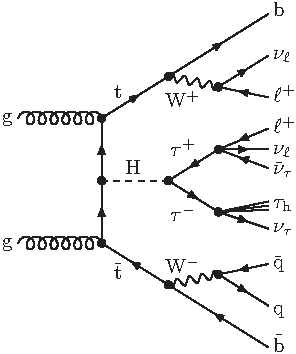
\includegraphics[width=0.30\linewidth]{diagrams/gg-ttH-tt-2lss.pdf} 
\hspace{0.5cm}
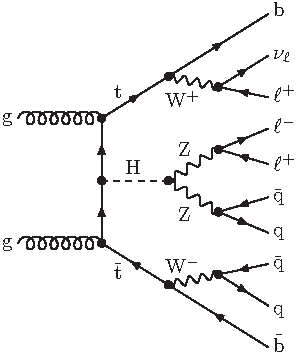
\includegraphics[width=0.30\linewidth]{diagrams/gg-ttH-ZZ-3l.pdf}
\hspace{0.5cm}
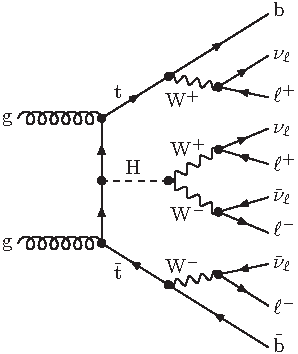
\includegraphics[width=0.30\linewidth]{diagrams/gg-ttH-WW-4l.pdf}
\caption{Examples of leading order Feynman diagrams for $t\bar{t}H$ production at pp colliders, with the Higgs boson decaying to
$\tau\tau$, $\mathrm{ZZ}^{*}$, and
$\mathrm{WW}^{*}$ (from left to right). The first, second, and third diagrams are examples of the two same-sign lepton signature,
the three lepton signature, and the four lepton signature, respectively.} 
\label{fig:feyn}
\end{figure}

\clearpage

\clearpage

\section{Data and MC Samples}
\label{sec:samples}
\subsection{Full 2016 dataset and MC samples}

The data considered in this analysis were collected by the CMS experiment during 2016 and correspond to a total integrated luminosity of 35.9\fbinv.
The data used were collected only in periods when the CMS magnet was on.
We use the 23 Sep 2016 (Run B to G) and PromptReco (Run H) versions of the datasets. 

The MC samples used in this analysis correspond to the RunIISummer16MiniAODv2 campaign produced with CMSSW 80X. 

The two signal samples (for \tHq\ and \tHW) were produced with \textsc{MG5\_}a\textsc{MC@NLO} (version 5.222), in leading-order order mode, and are normalized to next-to-leading-order cross sections, see Tab.~\ref{tab:sigsamples}.
Each sample is generated with a set of event weights corresponding to different values of \Ct\ and \CV\ couplings, see Tab.~\ref{tab:reweight}.

\begin{table}[h] 
  \centering
  \begin{tabular}{lll}
    Sample & $\sigma$ [pb] & BF \\
    \hline
    \verb|/THQ_Hincl_13TeV-madgraph-pythia8_TuneCUETP8M1/| & 0.7927 & 0.324 \\
    \verb|/THW_Hincl_13TeV-madgraph-pythia8_TuneCUETP8M1/| & 0.1472 & 1.0   \\
    \hline
  \end{tabular}
  \caption{Signal samples and their cross section and branching fraction used in this analysis. See Ref.~\cite{THQProdTwiki} for more details.}\label{tab:sigsamples}
\end{table}

\begin{table}[h!]
  \centering
  \footnotesize
  \begin{tabular}{lllllll}
        &       & \multicolumn{2}{c}{\tHq} & \multicolumn{2}{c}{\tHW} & \\\hline
   \CV\ & \Ct\  & sum of    & cross         & sum of    & cross        & \\
        &       & weights   & section [pb]  & weights   & section [pb] & LHE weights       \\\hline
   1.0  & -3.0  & 35.700022 & 2.991         & 11.030445 & 0.6409       & LHEweight\_wgt[446]\\
   1.0  & -2.0  & 20.124298 & 1.706         & 5.967205  & 0.3458       & LHEweight\_wgt[447]\\
   1.0  & -1.5  & 14.043198 & 1.205         & 4.029093  & 0.2353       & LHEweight\_wgt[448]\\
   1.0  & -1.25 & 11.429338 & 0.9869        & 3.208415  & 0.1876       & LHEweight\_wgt[449]\\
   1.0  & -1.0  &           & 0.7927        &           & 0.1472       & \\
   1.0  & -0.75 & 7.054998  & 0.6212        & 1.863811  & 0.1102       & LHEweight\_wgt[450]\\
   1.0  & -0.5  & 5.294518  & 0.4723        & 1.339886  & 0.07979      & LHEweight\_wgt[451]\\
   1.0  & -0.25 & 3.818499  & 0.3505        & 0.914880  & 0.05518      & LHEweight\_wgt[452]\\
   1.0  & 0.0   & 2.627360  & 0.2482        & 0.588902  & 0.03881      & LHEweight\_wgt[453]\\
   1.0  & 0.25  & 1.719841  & 0.1694        & 0.361621  & 0.02226      & LHEweight\_wgt[454]\\
   1.0  & 0.5   & 1.097202  & 0.1133        & 0.233368  & 0.01444      & LHEweight\_wgt[455]\\
   1.0  & 0.75  & 0.759024  & 0.08059       & 0.204034  & 0.01222      & LHEweight\_wgt[456]\\
   1.0  & 1.0   & 0.705305  & 0.07096       & 0.273617  & 0.01561      & LHEweight\_wgt[457]\\
   1.0  & 1.25  & 0.936047  & 0.0839        & 0.442119  & 0.02481      & LHEweight\_wgt[458]\\
   1.0  & 1.5   & 1.451249  & 0.1199        & 0.709538  & 0.03935      & LHEweight\_wgt[459]\\
   1.0  & 2.0   & 3.335034  & 0.2602        & 1.541132  & 0.08605      & LHEweight\_wgt[460]\\
   1.0  & 3.0   & 10.516125 & 0.8210        & 4.391335  & 0.2465       & LHEweight\_wgt[461]\\\hline
        &       &           &               &           &              & \\\hline
   1.5  & -3.0  & 45.281492 & 3.845         & 13.426212 & 0.7825       & LHEweight\_wgt[462]\\
   1.5  & -2.0  & 27.606715 & 2.371         & 7.809713  & 0.4574       & LHEweight\_wgt[463]\\
   1.5  & -1.5  & 20.476088 & 1.784         & 5.594971  & 0.3290       & LHEweight\_wgt[464]\\
   1.5  & -1.25 & 17.337465 & 1.518         & 4.635978  & 0.2749       & LHEweight\_wgt[465]\\
   1.5  & -1.0  & 14.483302 & 1.287         & 3.775902  & 0.2244       & LHEweight\_wgt[466]\\
   1.5  & -0.75 & 11.913599 & 1.067         & 3.014744  & 0.1799       & LHEweight\_wgt[467]\\
   1.5  & -0.5  & 9.628357  & 0.874         & 2.352505  & 0.1410       & LHEweight\_wgt[468]\\
   1.5  & -0.25 & 7.627574  & 0.702         & 1.789184  & 0.1081       & LHEweight\_wgt[469]\\
   1.5  & 0.0   & 5.911882  & 0.5577        & 1.324946  & 0.08056      & LHEweight\_wgt[470]\\
   1.5  & 0.25  & 4.479390  & 0.4365        & 0.959295  & 0.05893      & LHEweight\_wgt[471]\\
   1.5  & 0.5   & 3.331988  & 0.3343        & 0.692727  & 0.04277      & LHEweight\_wgt[472]\\
   1.5  & 0.75  & 2.469046  & 0.2558        & 0.525078  & 0.03263      & LHEweight\_wgt[473]\\
   1.5  & 1.0   & 1.890565  & 0.2003        & 0.456347  & 0.02768      & LHEweight\_wgt[474]\\
   1.5  & 1.25  & 1.596544  & 0.1689        & 0.486534  & 0.02864      & LHEweight\_wgt[475]\\
   1.5  & 1.5   & 1.586983  & 0.1594        & 0.615638  & 0.03509      & LHEweight\_wgt[476]\\
   1.5  & 2.0   & 2.421241  & 0.2105        & 1.170602  & 0.06515      & LHEweight\_wgt[477]\\
   1.5  & 3.0   & 7.503280  & 0.5889        & 3.467546  & 0.1930       & LHEweight\_wgt[478]\\\hline
        &       &           &               &           & \\ \hline
   0.5  & -3.0  & 27.432685 & 2.260         & 8.929074  & 0.5136       & LHEweight\_wgt[479]\\
   0.5  & -2.0  & 13.956013 & 1.160         & 4.419093  & 0.2547       & LHEweight\_wgt[480]\\
   0.5  & -1.5  & 8.924438  & 0.7478        & 2.757611  & 0.1591       & LHEweight\_wgt[481]\\
   0.5  & -1.25 & 6.835341  & 0.5726        & 2.075247  & 0.1204       & LHEweight\_wgt[482]\\
   0.5  & -1.0  & 5.030704  & 0.4273        & 1.491801  & 0.08696      & LHEweight\_wgt[483]\\
   0.5  & -0.75 & 3.510528  & 0.2999        & 1.007273  & 0.05885      & LHEweight\_wgt[484]\\
   0.5  & -0.5  & 2.274811  & 0.1982        & 0.621663  & 0.03658      & LHEweight\_wgt[485]\\
   0.5  & -0.25 & 1.323555  & 0.1189        & 0.334972  & 0.01996      & LHEweight\_wgt[486]\\
   0.5  & 0.0   & 0.656969  & 0.06223       & 0.147253  & 0.008986     & LHEweight\_wgt[487]\\
   0.5  & 0.25  & 0.274423  & 0.02830       & 0.058342  & 0.003608     & LHEweight\_wgt[488]\\
   0.5  & 0.5   & 0.176548  & 0.01778       & 0.068404  & 0.003902     & LHEweight\_wgt[489]\\
   0.5  & 0.75  & 0.363132  & 0.03008       & 0.177385  & 0.009854     & LHEweight\_wgt[490]\\
   0.5  & 1.0   & 0.834177  & 0.06550       & 0.385283  & 0.02145      & LHEweight\_wgt[491]\\
   0.5  & 1.25  & 1.589682  & 0.1241        & 0.692099  & 0.03848      & LHEweight\_wgt[492]\\
   0.5  & 1.5   & 2.629647  & 0.2047        & 1.097834  & 0.06136      & LHEweight\_wgt[493]\\
   0.5  & 2.0   & 5.562958  & 0.4358        & 2.206057  & 0.1246       & LHEweight\_wgt[494]\\
   0.5  & 3.0   & 14.843102 & 1.177         & 5.609519  & 0.3172       & LHEweight\_wgt[495]\\ \hline
    \end{tabular} 
    \caption{\CV\ and \Ct\ combinations generated for the two signal samples and their NLO cross sections. The \tHq\ cross section is multiplied by the branching fraction of the enforced leptonic decay of the top quark (0.324). See also Ref.~\cite{THQProdTwiki}.}\label{tab:reweight}
 \end{table}

Different MC generators were used to generate the background processes.
The dominant sources (\ttbar, \ttW, \ttZ, \ttH) were produced using \textsc{aMC@NLO} interfaced to \PYTHIA8, and are scaled to NLO cross sections.
Other processes are simulated using \POWHEG\ interfaced to \PYTHIA, or bare \PYTHIA.
See table~\ref{tab:bgsamples} for more details.
See also AN-2016-211 (Ref.~\cite{CMS_AN_2016-211}) for more details.

\begin{table}
\footnotesize
\centering
\begin{tabular}{ll}
	Sample & $\sigma$ [pb] \\
	\hline
	\verb|TTWJetsToLNu_TuneCUETP8M1_13TeV-amcatnloFXFX-madspin-pythia8|           & 0.2043 \\
	\verb|TTZToLLNuNu_M-10_TuneCUETP8M1_13TeV-amcatnlo-pythia8|                   & 0.2529 \\
	\verb|ttHJetToNonbb_M125_13TeV_amcatnloFXFX_madspin_pythia8_mWCutfix|         & 0.2151 \\
	\verb|/store/cmst3/group/susy/gpetrucc/13TeV/u/TTLL_m1to10_LO_NoMS_for76X/|   & 0.0283 \\
	\verb|WGToLNuG_TuneCUETP8M1_13TeV-madgraphMLM-pythia8|                        & 585.8 \\
	\verb|ZGTo2LG_TuneCUETP8M1_13TeV-amcatnloFXFX-pythia8|                        & 131.3 \\
	\verb|TGJets_TuneCUETP8M1_13TeV_amcatnlo_madspin_pythia8|                     & 2.967 \\
	\verb|TTGJets_TuneCUETP8M1_13TeV-amcatnloFXFX-madspin-pythia8|                & 3.697 \\
	\verb|WpWpJJ_EWK-QCD_TuneCUETP8M1_13TeV-madgraph-pythia8|                     & 0.03711 \\
	\verb|ZZZ_TuneCUETP8M1_13TeV-amcatnlo-pythia8|                                & 0.01398 \\
	\verb|WWZ_TuneCUETP8M1_13TeV-amcatnlo-pythia8|                                & 0.1651 \\
	\verb|WZZ_TuneCUETP8M1_13TeV-amcatnlo-pythia8|                                & 0.05565 \\
	\verb|WW_DoubleScattering_13TeV-pythia8|                                      & 1.64 \\
	\verb|tZq_ll_4f_13TeV-amcatnlo-pythia8_TuneCUETP8M1|                          & 0.0758 \\
	\verb|ST_tWll_5f_LO_13TeV-MadGraph-pythia8|                                   & 0.01123 \\
	\verb|TTTT_TuneCUETP8M1_13TeV-amcatnlo-pythia8|                               & 0.009103 \\
	\verb|WZTo3LNu_TuneCUETP8M1_13TeV-powheg-pythia8|                             & 4.4296 \\
	\verb|ZZTo4L_13TeV_powheg_pythia8|                                            & 1.256 \\
	\hline
	\verb|TTJets_SingleLeptFromTbar_TuneCUETP8M1_13TeV-madgraphMLM-pythia8|       & 182.1754 \\
	\verb|TTJets_SingleLeptFromT_TuneCUETP8M1_13TeV-madgraphMLM-pythia8|          & 182.1754 \\
	\verb|TTJets_DiLept_TuneCUETP8M1_13TeV-madgraphMLM-pythia8|                   & 87.3 \\
	\verb|DYJetsToLL_M-10to50_TuneCUETP8M1_13TeV-amcatnloFXFX-pythia8|            & 18610 \\
	\verb|DYJetsToLL_M-50_TuneCUETP8M1_13TeV-madgraphMLM-pythia8|                 & 6024 \\
	\verb|WJetsToLNu_TuneCUETP8M1_13TeV-amcatnloFXFX-pythia8|                     & 61526.7 \\
	\verb|ST_tW_top_5f_inclusiveDecays_13TeV-powheg-pythia8_TuneCUETP8M1|         & 35.6 \\
	\verb|ST_tW_antitop_5f_inclusiveDecays_13TeV-powheg-pythia8_TuneCUETP8M1|     & 35.6 \\
	\verb|ST_t-channel_4f_leptonDecays_13TeV-amcatnlo-pythia8_TuneCUETP8M1|       & 70.3144\\
	\verb|ST_t-channel_antitop_4f_leptonDecays_13TeV-powheg-pythia8_TuneCUETP8M1| & 26.2278\\
	\verb|ST_s-channel_4f_leptonDecays_13TeV-amcatnlo-pythia8_TuneCUETP8M1|       & 3.68064 \\
	\verb|WWTo2L2Nu_13TeV-powheg|                                                 & 10.481 \\
	\hline
\end{tabular}
\caption{List of background samples used in this analysis (CMSSW
  80X). In the first section of the table are listed the samples of
  the processes for which we use the simulation to extract the final
  yields and shapes, in the second section the samples of the
  processes we will estimate from data. The MC simulation is used to
  design the data driven methods and derive the associated systematics.} \label{tab:bgsamples}
\end{table}

\begin{table}
\centering
\begin{tabular}{ll}
	Sample & $\sigma$ [pb] \\
	\hline
	\verb|ttWJets_13TeV_madgraphMLM| & 0.6105 \\
	\verb|ttZJets_13TeV_madgraphMLM| & 0.5297/0.692 \\
	\hline
\end{tabular}
\caption{Leading-order \ttW\ and \ttZ\ samples used in the signal BDT training.} \label{tab:ttvlo_samples}
\end{table}

\subsection{Triggers}
We consider online-reconstructed events triggered by one, two, or three leptons.
Single-lepton triggers are included to boost the acceptance of events where the \pt\ of the sub-leading lepton falls below the threshold of the double-lepton triggers.
Additionally, by including double-lepton triggers in the $\geq$ 3 lepton category, as well as single-lepton triggers in all categories, we increase the efficiency, considering the logical ``or'' of the trigger decisions of all the individual triggers in a given category.
Tab.~\ref{tab:triggers} shows the lowest-threshold non-prescaled triggers present in the High-Level Trigger (HLT) menus for both Monte-Carlo and data in 2016.

\begin{table}[h]
\centering
	\begin{tabular}{l}
    \hline
    Same-sign dilepton (==2 muons)\\
    \verb|HLT_Mu17_TrkIsoVVL_Mu8_TrkIsoVVL_DZ_v*|\\
    \verb|HLT_Mu17_TrkIsoVVL_TkMu8_TrkIsoVVL_DZ_v*|\\
    \verb|HLT_IsoMu22_v*|\\
    \verb|HLT_IsoTkMu22_v*|\\
    \verb|HLT_IsoMu22_eta2p1_v*| \\
    \verb|HLT_IsoTkMu22_eta2p1_v*| \\
    \verb|HLT_IsoMu24_v*| \\
    \verb|HLT_IsoTkMu24_v*|\\\hline
    Same-sign dilepton (==2 electrons)\\
    \verb|HLT_Ele23_Ele12_CaloIdL_TrackIdL_IsoVL_DZ_v*|\\
    \verb|HLT_Ele27_eta2p1_WPLoose_Gsf_v*|\\
    \verb|HLT_Ele27_WPTight_Gsf_v*| \\
    \verb|HLT_Ele25_eta2p1_WPTight_Gsf_v*| \\\hline
    Same-sign dilepton (==1 muon, ==1 electron)\\
    \verb|HLT_Mu23_TrkIsoVVL_Ele8_CaloIdL_TrackIdL_IsoVL_v*|\\
    \verb|HLT_Mu8_TrkIsoVVL_Ele23_CaloIdL_TrackIdL_IsoVL_v*|\\
    \verb|HLT_Mu23_TrkIsoVVL_Ele8_CaloIdL_TrackIdL_IsoVL_DZ_v*| \\
    \verb|HLT_Mu8_TrkIsoVVL_Ele23_CaloIdL_TrackIdL_IsoVL_DZ_v*| \\
    \verb|HLT_IsoMu22_v*|\\
    \verb|HLT_IsoTkMu22_v*|\\
    \verb|HLT_IsoMu22_eta2p1_v*| \\
    \verb|HLT_IsoTkMu22_eta2p1_v*| \\
    \verb|HLT_IsoMu24_v*| \\
    \verb|HLT_IsoTkMu24_v*| \\
    \verb|HLT_Ele27_WPTight_Gsf_v*| \\
    \verb|HLT_Ele25_eta2p1_WPTight_Gsf_v*| \\
    \verb|HLT_Ele27_eta2p1_WPLoose_Gsf_v*|\\\hline
    Three lepton and Four lepton\\
    \verb|HLT_DiMu9_Ele9_CaloIdL_TrackIdL_v*|\\
    \verb|HLT_Mu8_DiEle12_CaloIdL_TrackIdL_v*|\\
    \verb|HLT_TripleMu_12_10_5_v*|\\
    \verb|HLT_Ele16_Ele12_Ele8_CaloIdL_TrackIdL_v*|\\
    \verb|HLT_Mu23_TrkIsoVVL_Ele8_CaloIdL_TrackIdL_IsoVL_v*|\\
    \verb|HLT_Mu23_TrkIsoVVL_Ele8_CaloIdL_TrackIdL_IsoVL_DZ_v*| \\
    \verb|HLT_Mu8_TrkIsoVVL_Ele23_CaloIdL_TrackIdL_IsoVL_v*|\\
    \verb|HLT_Mu8_TrkIsoVVL_Ele23_CaloIdL_TrackIdL_IsoVL_DZ_v|* \\
    \verb|HLT_Ele23_Ele12_CaloIdL_TrackIdL_IsoVL_DZ_v*|\\
    \verb|HLT_Mu17_TrkIsoVVL_Mu8_TrkIsoVVL_DZ_v*|\\
    \verb|HLT_Mu17_TrkIsoVVL_TkMu8_TrkIsoVVL_DZ_v*|\\
    \verb|HLT_IsoMu22_v*|\\
    \verb|HLT_IsoTkMu22_v*|\\
    \verb|HLT_IsoMu22_eta2p1_v*|\\
    \verb|HLT_IsoTkMu22_eta2p1_v*|\\
    \verb|HLT_IsoMu24_v*|\\
    \verb|HLT_IsoTkMu24_v*|\\
    \verb|HLT_Ele27_WPTight_Gsf_v*|\\
    \verb|HLT_Ele25_eta2p1_WPTight_Gsf_v*|\\
    \verb|HLT_Ele27_eta2p1_WPLoose_Gsf_v*|\\
	\hline
    \end{tabular}
    \caption{Table of high-level triggers that we consider in the analysis.} \label{tab:triggers}
\end{table}

\subsubsection{Trigger efficiency scale factors}
The efficiency of events to pass the trigger is measured in simulation (trivially using generator information) and in the data (using event collected by an uncorrelated MET trigger).
Small differences between the data and MC efficiencies are corrected by applying scale factors as shown in Tab.~\ref{tab:trigSFs}.
The exact procedure and control plots are documented in Refs~\cite{CMS_AN_2016-211} (for the ICHEP dataset), and in~\cite{CMS_AN_2017-029} for the current analysis.

\begin{table}
\centering
\begin{tabular}{ll}
	Category & Scale Factor \\
	\hline
	ee       & $1.01 \pm 0.02$ \\
	e$\mu$   & $1.01 \pm 0.01$ \\
	$\mu\mu$ & $1.00 \pm 0.01$ \\
	3l       & $1.00 \pm 0.03$ \\
	\hline
\end{tabular}
\caption{Trigger efficiency scale factors and associated uncertainties, shown here rounded to the nearest percent.}
\label{tab:trigSFs}
\end{table}

\clearpage

\section{Object identification and event selection}
\label{sec:objects}
\subsection{Jets and \cPqb\ tagging}
The analysis uses anti-\kt\ (0.4) particle-flow (PF) jets, corrected for charged hadrons not coming from the primary vertex (charged hadron subtraction), and having jet energy corrections (\verb|Summer16_23Sep2016V3|) applied as a function of the jet $E_T$ and $\eta$.
Jets are only considered if they have a transverse energy above $25\GeV$.
% FIXME Something about forward jets?

In addition, they are required to be separated from any lepton candidates passing the fakeable object selections (see Tables~\ref{tab:muonIDs} and~\ref{tab:eleIDs}) by $\Delta\mathrm{R}>0.4$.

The loose and medium working points of the CSV \cPqb-tagging algorithm are used to identify \cPqb\ jets.
Data/simulation differences in the \cPqb\ tagging performance are corrected by applying per-jet weights to the simulation, dependent on the jet \pt, eta, \cPqb\ tagging discriminator, and flavor (from simulation truth)~\cite{btagRecommTWiki}.
The per-event weight is taken as the product of the per-jet weights, including those of the jets associated to the leptons.

More details can be found in the corresponding \ttH\ documentation~\cite{CMS_AN_2016-211,CMS_AN_2017-029}.

\subsection{Lepton selection}
The lepton reconstruction and selection is identical to that used in the \ttH\ multilepton analysis, as documented in Refs.~\cite{CMS_AN_2016-211,CMS_AN_2017-029}.
For details on the reconstruction algorithms, isolation, pileup mitigation, and a description of the lepton MVA discriminator and validation plots thereof, we refer to that document.

Three different selections are defined both for the electron and muon
object identification: the \emph{Loose}, \emph{Fakeable Object},
and \emph{Tight} selection.
As described in more detail later, these are used for event level vetoes, the fake rate estimation application region, and the final signal selection, respectively.
The \pt\ of fakeable objects is defined as $0.85\times\pt(\mathrm{jet})$, where the jet is the one associated to the lepton object.
This mitigates the dependence of the fake rate on the momentum of the fakeable object and thereby improves the precision of the method.

Tables~\ref{tab:muonIDs} and~\ref{tab:eleIDs} list the full criteria for the different selections of muons and electrons.

\begin{table}[h!]
\centering
\small
\topcaption{
\label{tab:muonIDs}
Requirements on each of the three muon selections. In the cases where
the cut values change between the selections, those values are listed in the table.
Otherwise, whether the cut is applied is indicated.
For the two \ptRatio\ and CSV rows, the cuts marked with a $\dagger$ are applied to leptons that fail the lepton MVA cut, while the loose cut value is applied to those that pass the lepton MVA cut.}
\begin{tabular}{cccc}
Cut & Loose & Fakeable object & Tight \\
\hline
$|\eta| < 2.4$         & \checkmark & \checkmark         & \checkmark \\
$\pt$                  & $>5\GeV$   & $>15\GeV$          & $>15\GeV$\\
$|d_{xy}| < 0.05$ (cm) & \checkmark & \checkmark         & \checkmark \\
$|d_z| < 0.1$ (cm)     & \checkmark & \checkmark         & \checkmark \\
$\text{SIP}_{3D} < 8$  & \checkmark & \checkmark         & \checkmark \\
\miniIso $< 0.4$       & \checkmark & \checkmark         & \checkmark \\
is Loose Muon          & \checkmark & \checkmark         & \checkmark \\
%\ptRatio              & --         & $>0.3\dagger$ / -- & -- \\
jet CSV                & --         & $< 0.8484$         & $ < 0.8484$ \\
%mva electron ID       & --         & $\ddagger$         & -- \\
is Medium Muon         & --         & --                 & \checkmark \\
tight-charge           & --         & --                 & \checkmark \\
lepMVA $> 0.90$        & --         & --                 & \checkmark \\
\hline
\end{tabular}
\end{table}


\begin{table}
\centering
\small
\topcaption{
\label{tab:eleIDs}
Criteria for each of the three electron selections. In cases where the cut values change between selections, those values are listed in the table. Otherwise, whether the cut is applied is indicated. In some cases, the cut values change for different $\eta$ ranges. These ranges are $0 < |\eta| < 0.8$, $0.8 < |\eta| < 1.479$, and $1.479 < |\eta| < 2.5$ and the respective cut values are given in the form (value$_1$, value$_2$, value$_3$).
}
\resizebox{1.0\linewidth}{!}{
\begin{tabular}{cccc}
Cut & Loose & Fakeable Object & Tight \\
\hline
$|\eta| < 2.5$                                  & \checkmark & \checkmark                   & \checkmark \\
$\pt$                                           & $>7\GeV$   & $>15\GeV$                    & $>15\GeV$      \\
$|d_{xy}| < 0.05$ (cm)                          & \checkmark & \checkmark                   & \checkmark \\
$|d_z| < 0.1$ (cm)                              & \checkmark & \checkmark                   & \checkmark \\
$\text{SIP}_{3D} < 8$                           & \checkmark & \checkmark                   & \checkmark \\
\miniIso $< 0.4$                                & \checkmark & \checkmark                   & \checkmark \\
MVA ID $> (0.0, 0.0, 0.7)$                      & \checkmark & \checkmark                   & \checkmark \\
$\sigma_{i\eta i\eta} <(0.011,0.011,0.030)$     & --         & \checkmark                   & \checkmark \\ %   & for corr. $\pt>30$ & for corr. $\pt>30$ \\
H/E $< (0.10,0.10,0.07)$                        & --         & \checkmark                   & \checkmark \\ %   & for corr. $\pt>30$ & for corr. $\pt>30$ \\
$\Delta\eta_{\textrm in} < (0.01, 0.01, 0.008)$ & --         & \checkmark                   & \checkmark \\ %   & for corr. $\pt>30$ & for corr. $\pt>30$ \\
$\Delta\phi_{\textrm in} < (0.04, 0.04, 0.07)$  & --         & \checkmark                   & \checkmark \\ %   & for corr. $\pt>30$ & for corr. $\pt>30$ \\
$-0.05 < 1/E-1/p < (0.010,0.010,0.005)$         & --         & \checkmark                   & \checkmark \\ %   & for corr. $\pt>30$ & for corr. $\pt>30$ \\
\ptRatio                                        & --         & $>0.5\dagger$ / --           & -- \\
jet CSV                                         & --         & $< 0.3 \dagger$ / $< 0.8484$ & $ < 0.8484$ \\
tight-charge                                    & --         & --                           & \checkmark \\
conversion rejection                            & --         & --                           & \checkmark \\
Number of missing hits                          & $<2$       & $== 0$                       & $== 0$ \\
lepMVA $> 0.90$                                 & --         & --                           & \checkmark \\
\hline
\end{tabular}}
\end{table}


\subsection{Lepton selection efficiency}
Efficiencies of reconstruction and selecting loose leptons are measured both for muons and electrons using a tag and probe method on both data and MC, using $Z\rightarrow\ell^{+}\ell^{-}$.
Corresponding scale factors are derived from the ratio of efficiencies and applied to the selected events.
These are produced for the leptonic SUSY analyses using equivalent lepton selections and recycled for the \ttH\ analysis as well as for this analysis.

The efficiencies of applying the tight selection as defined in Tables~\ref{tab:muonIDs} and~\ref{tab:eleIDs}, on the loose leptons are determined again by using a tag and probe method on a sample of DY-enriched events.
They are documented for the \ttH\ analysis in Ref.~\cite{CMS_AN_2017-029} and are exactly equivalent for this analysis.


\subsection{Event selection}
Events are selected considering the features of the signal process and the decay signatures.

At least two same-sign or three leptons of any sign, passing the tight selection are required.
In the dilepton channels, events are vetoed if they contain additional tight leptons.

Events are required to have fired one of the corresponding trigger paths, and are vetoed if any loose lepton pair has an invariant mass below $12\GeV$.

In the dilepton channels, the leptons are required to have $\pt>25\GeV$ for the leading, and $\pt>15\GeV$ for the sub-leading lepton.
In the three lepton channel, they are required to have respectively $\pt>25\GeV$, $>15\GeV$, and $>15\GeV$.

Three lepton events with an opposite-sign, same-flavor lepton combination with invariant mass within 15\GeV\ of the \Z\ boson mass are discarded to reject events from \WZ+jets production.
Same-sign di-electron events where the two electrons have invariant mass within 10\GeV\ of the \Z\ boson mass are equally discarded to reject events from DY+jets production with charge mis-identified electrons.

Leptons in the three lepton channel are not required to pass the triple charge consistency criteria (for electrons), or the $\Delta{\pt}/\pt <0.2$ cut (for muons).

Furthermore we require at least two jets of which at least one passes the medium \cPqb\ tagging working point ($\pt>25\GeV$ and $|\eta|<2.4$), and at least one not passing the loose working point ($\pt>25\GeV$ for $|\eta|<2.4$ and $\pt>40\GeV$ for $|\eta|>2.4$).

The event selection is summarized in Tab~\ref{tab:evsel}.

\begin{table}[h!]
\centering
\begin{tabular}{c|c}
	\hline
	\multicolumn{2}{c}{No loose leptons with $m_{\ell\ell} < 12\GeV$} \\
	%\multicolumn{2}{c}{Two or more jets with $\pt>25\GeV$} \\
	\multicolumn{2}{c}{One or more jets passing CSV medium ($|\eta|<2.4$)} \\
	\multicolumn{2}{c}{One or more jets failing CSV loose} \\
	\hline
	Exactly two tight same-sign leptons & Exactly three tight leptons \\
	$\pt>25/15\GeV$ & $\pt>25/15/15\GeV$ \\
	No \Pe\Pe\ events with $|m_{\Pe\Pe}-m_\Z|<10\GeV$ & No OSSF pair with $|m_{\ell\ell}-m_\Z|<15\GeV$ \\
	Triple charge consistent electrons &  \\
	Muons with $\Delta{\pt}/\pt <0.2$ &  \\
	\hline
\end{tabular}
\caption{Summary of event selection.}\label{tab:evsel}
\end{table}

\begin{table}[thb]
\centering
\begin{tabular}{lrrrr}
\multicolumn{1}{c@{\qquad}}{} &
\multicolumn{1}{c@{\qquad}}{$3\ell$} &
\multicolumn{1}{c}{$\Pgm\Pgm$} &
\multicolumn{1}{c@{\qquad}}{$\Pe\Pgm$} &
\multicolumn{1}{c}{$\Pe\Pe$} \\ \hline
$\ttW$                        & $  22.50 \pm 0.35$ & $ 68.03 \pm 0.61 $ & $ 97.00 \pm 0.71 $ & $ 29.63 \pm  0.39 $ \\
$\ttZ\!/\!\gamma^*$           & $  32.80 \pm 1.79$ & $ 25.89 \pm 1.12 $ & $ 64.82 \pm 2.42 $ & $ 28.74 \pm  1.70 $ \\
$\WZ$                         & $   8.22 \pm 0.86$ & $ 15.07 \pm 1.19 $ & $ 26.25 \pm 1.57 $ & $  9.31 \pm  0.93 $ \\
$\ZZ$                         & $   1.62 \pm 0.33$ & $  1.16 \pm 0.29 $ & $  2.86 \pm 0.45 $ & $  1.09 \pm  0.27 $ \\
$\PW^\pm\PW^\pm\cPq\cPq$      & --                 & $  3.96 \pm 0.52 $ & $  6.99 \pm 0.69 $ & $  2.19 \pm  0.37 $ \\
$\PW^\pm\PW^\pm \text{(DPS)}$ & --                 & $  2.48 \pm 0.42 $ & $  4.17 \pm 0.54 $ & $  0.81 \pm  0.24 $ \\
VVV                           & $   0.42 \pm 0.16$ & $  2.99 \pm 0.34 $ & $  4.85 \pm 0.43 $ & $  1.19 \pm  0.21 $ \\
$\mathrm{tttt}$               & $   1.84 \pm 0.44$ & $  2.32 \pm 0.45 $ & $  4.06 \pm 0.57 $ & $  0.89 \pm  0.31 $ \\
$\mathrm{tZq}$                & $   3.92 \pm 1.48$ & $  5.77 \pm 2.24 $ & $ 10.73 \pm 3.03 $ & $  7.56 \pm  1.72 $ \\
$\mathrm{tZW}$                & $   1.70 \pm 0.12$ & $  2.13 \pm 0.13 $ & $  3.91 \pm 0.18 $ & $  1.13 \pm  0.10 $ \\
$\gamma$ conversions          & $   7.43 \pm 1.94$ & --                 & $ 23.81 \pm 6.04 $ & $  9.87 \pm  4.17 $ \\ \hline
Non-prompt                    & $  25.61 \pm 1.26$ & $ 80.94 \pm 2.02 $ & $135.34 \pm 2.83 $ & $ 47.72 \pm  1.79 $ \\
Charge mis-ID                 & --                 & --                 & $ 58.50 \pm 0.31 $ & $ 44.52 \pm  0.31 $ \\ \hline
All backgrounds               & $ 106.05 \pm 3.45$ & $210.74 \pm 3.61 $ & $443.30 \pm 8.01 $ & $184.65 \pm  5.29 $ \\ \hline
$\tHq$ ($\Ct=-1.0$)           & $   7.48 \pm 0.14$ & $ 18.48 \pm 0.22 $ & $ 27.41 \pm 0.27 $ & $  8.47 \pm  0.15 $ \\
$\tHW$ ($\CV=-1.0$)           & $   7.38 \pm 0.16$ & $  7.72 \pm 0.17 $ & $ 11.23 \pm 0.20 $ & $  3.66 \pm  0.11 $ \\
$\ttH$                        & $  18.29 \pm 0.41$ & $ 24.18 \pm 0.48 $ & $ 35.21 \pm 0.58 $ & $ 11.07 \pm  0.32 $ \\ \hline
Data (35.9\fbinv)             & \multicolumn{1}{l}{149}&\multicolumn{1}{l}{280} & \multicolumn{1}{l}{525} & \multicolumn{1}{l}{208}               \\
\end{tabular}
\caption{Expected and observed yields for $35.9\fbinv$ after the selection in all final states. Uncertainties are statistical only.}
\label{tab:yields-sel}
\end{table}

In the multi-leptonic final states of the signal processes, the largest contribution is from Higgs decays to $\PW\PW$, $\sim 75\%$ of the time, as shown in Tab~\ref{tab:yield_hbr}.
This is followed by the $\tau \tau$ and $ZZ$ decay modes respectively.
A minor contribution is also there from Higgs to $\mu \mu$ and $\gamma \gamma$ decays.

\begin{table}[HBR]
\centering
\begin{tabular}{lrrrr}
\multicolumn{1}{c@{\qquad}}{} &
\multicolumn{2}{c@{\qquad}}{$3\ell$} &
\multicolumn{2}{c}{$\Pgm\Pgm$} \\ \hline
$\tHq (\mathrm{Inclusive})$  & $\mathbf{6.57}$ & 100.0\% & $\mathbf{17.38}$ & 100.0\% \\
$\tHq (\PH\to \PW\PW)$       & $4.84$  & 73.9\%   & $13.33 $ &  76.9\%  \\
$\tHq (\PH\to \tau\tau)$     & $1.04$  & 15.9\%   & $ 3.62 $ &  20.6\%  \\
$\tHq (\PH\to \Z\Z)$         & $0.48$  &  7.2\%   & $ 0.37 $ &   2.2\%  \\
$\tHq (\PH\to \mu\mu)$       & $0.21$  &  3.0\%   & $ 0.04 $ &   0.2\%  \\
$\tHq (\PH\to \gamma\gamma)$ & $<0.01$ &  0.1\%   & $ 0.02 $ &   0.1\%  \\
$\tHq (\PH\to \cPqb\cPqb)$   & $<0.01$ & $<0.1$\% & $ 0.01 $ & $<0.1$\% \\ \hline
$\tHW (\mathrm{Inclusive})$  & $\mathbf{7.32}$ & 100.0\% & $\mathbf{7.62}$ & 100.0\% \\
$\tHW (\PH\to \PW\PW)$       & $5.50 $ &  76.9\%  & $ 5.60$ & 74.1\% \\
$\tHW (\PH\to \tau\tau)$     & $1.40 $ &  20.6\%  & $ 1.81$ & 23.1\% \\
$\tHW (\PH\to \Z\Z)$         & $0.31 $ &   2.2\%  & $ 0.21$ &  2.7\% \\
$\tHW (\PH\to \mu\mu)$       & $0.12 $ &   0.2\%  & $ 0.01$ &  0.1\% \\
$\tHW (\PH\to \gamma\gamma)$ & $<0.01$ & $<0.1$\% & $<0.01$ &$<0.1$\% \\
$\tHW (\PH\to \cPqb\cPqb)$   & $<0.01$ & $<0.1$\% & $<0.01$ &$<0.1$\% \\ \hline
\end{tabular}
\caption{Signal yields split by decay channels of the Higgs boson. (Note that these numbers are with a forward jet $\pt$ cut at 25\GeV.)}
\label{tab:yield_hbr}
\end{table}

\clearpage

\section{Background predictions}
\label{sec:backgrounds}
The modeling of reducible and irreducible backgrounds in this analysis uses the exact methods, analysis code, and ROOT trees used for the \ttH\ multilepton analysis which is being finalized concurrently.
We give a brief description of the methods and refer to the documentation of that analysis in Refs.~\cite{CMS_AN_2016-211,CMS_AN_2017-029} for any details.

The backgrounds in three-lepton and same-sign dilepton final states can be split in two broad categories: irreducible backgrounds with genuine prompt leptons (\ie\ from on-shell \PW\ and \Z\ boson decays); and reducible backgrounds where at least one of the leptons is ``non-prompt'', \ie\ produced within a hadronic jet, either a genuine lepton from heavy flavor decays, or simply mis-reconstructed jets.
A further class of reducible backgrounds consists of leptons with a mis-reconstructed electric charge sign, only truly relevant for electrons.

Irreducible backgrounds can be reliantly estimated directly from Monte-Carlo simulated events, using higher-order cross sections or data control regions for the overall normalization.
This is done in this analysis for all backgrounds involving prompt leptons: \ttW, \ttZ, \ttH, \WZ, $\Z\Z$, $\PW^\pm\PW^\pm\cPq\cPq$, $\cPqt\cPaqt\cPqt\cPaqt$, $\cPqt\Z\cPq$, $\cPqt\Z\PW$, $\PW\PW\PW$, $\PW\PW\Z$, $\PW\Z\Z$, $\Z\Z\Z$.

Reducible backgrounds, on the other hand, are not well predicted by simulation, and are estimated using data-driven methods.
In the case of non-prompt leptons, a fake rate method is used where the contribution to the final selection is estimated by extrapolating from a sideband (or ``application region'') with a looser lepton definition (the fakeable object definitions in Tabs.~\ref{tab:muonIDs} and~\ref{tab:eleIDs}) to the signal selection.
The tight-to-loose ratios (or ``fake rates'') are measured in several background dominated data events with dedicated triggers, subtracting the residual prompt lepton contribution using MC.\@
Non-prompt leptons in our signal regions are predominantly produced in \ttbar\ events, with a much smaller contribution, mainly in the three-lepton channel, from Drell--Yan production.
The systematic uncertainty on the normalization of the non-prompt background estimation is on the order of 50\%, and thereby one of the dominant limitations on the performance of multilepton analyses in general and this analysis in particular.
It consists of several individual sources, such as the result of closure tests of the method using simulated events, limited statistics in the data control regions due to necessary prescaling of lepton triggers, and the uncertainty in the subtraction of residual prompt leptons from the control region.

The fake background where the leptons pass the looser selection are weighted according to how many of them fail the tight criteria.   
Events with a single failing lepton are weighted with the factor $f/(1-f)$ for the estimate to the tight selection region, where $f$ is the fake rate. 
Events with two failing leptons are given the negative weight $-f_{i}f_{j}/(1-f_{i})(1-f_{j})$, and for three leptons the weight is positive and equal to the product of $f/(1-f)$ factor evaluated for each failing lepton.

Finally, backgrounds from electron charge mis-identification (muon charge mis-id.\ is negligible) are estimated from the yield of opposite-sign event in the signal region using a measured charge mis-identification probability.
The mis-id.\ probability is measured in same-sign and opposite-sign Drell--Yan events, in several bins of \pt\ and $\eta$.
As for non-prompt leptons, the contribution from charge mis-identified electrons in our signal selection is predominantly from \ttbar\ and Drell--Yan events.
The systematic uncertainty of the normalization of the charge mis-id.\ estimate is evaluated at about 30\%, stemming from a slight disagreement of the mis-id.\ probability between data and simulation.
As it only affects the \Pe\Pgm\ channel, however, the impact of this background on the final sensitivity is very limited.

Figures~\ref{fig:input_vars_3l_xsec}, \ref{fig:input_vars_2lss_xsec_mumu} and~\ref{fig:input_vars_2lss_xsec_emu} show the distributions of some relevant kinematic variables, normalized to the cross section of the respective processes and to the integrated luminosity.
\begin{figure} [!h]
 \centering
 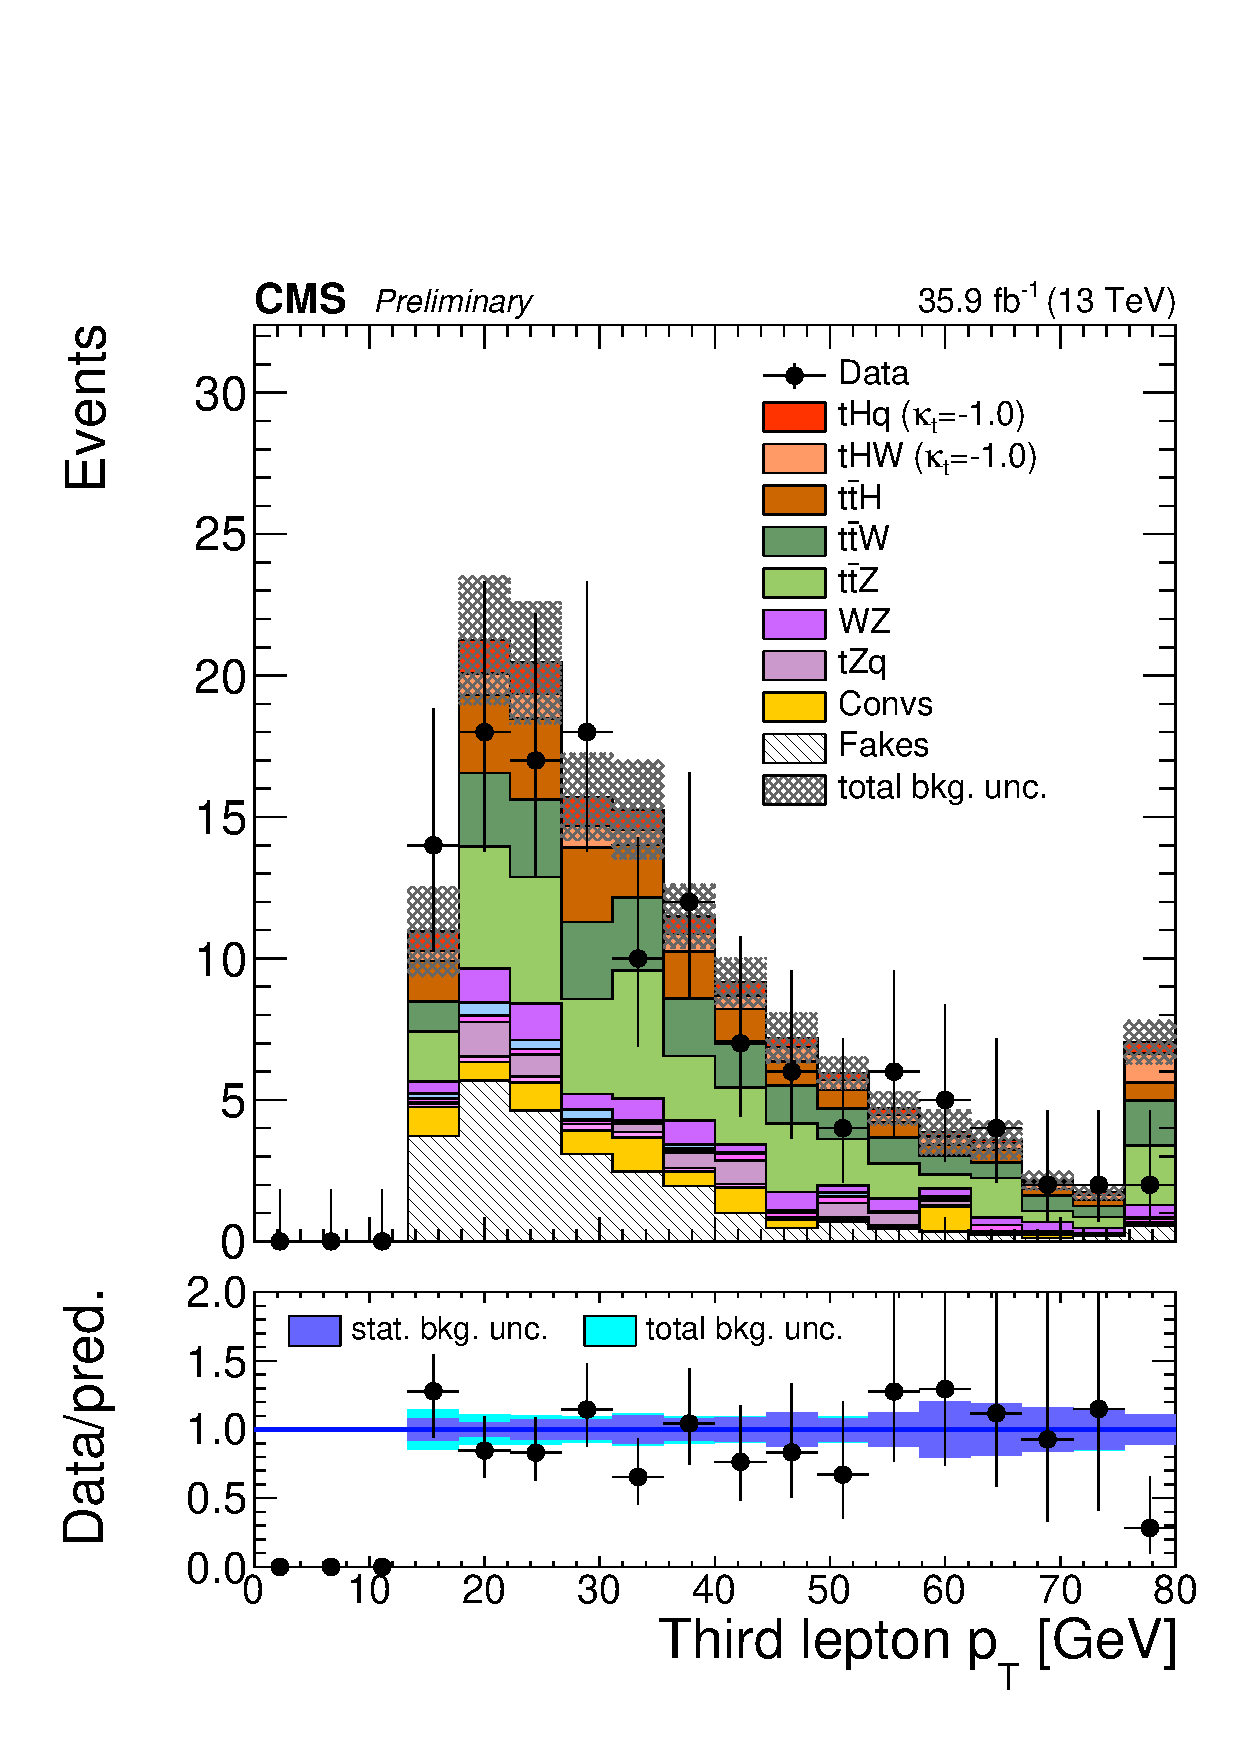
\includegraphics[width=0.22\textwidth]{figures/3lsignal/Lep3Pt.pdf} 
 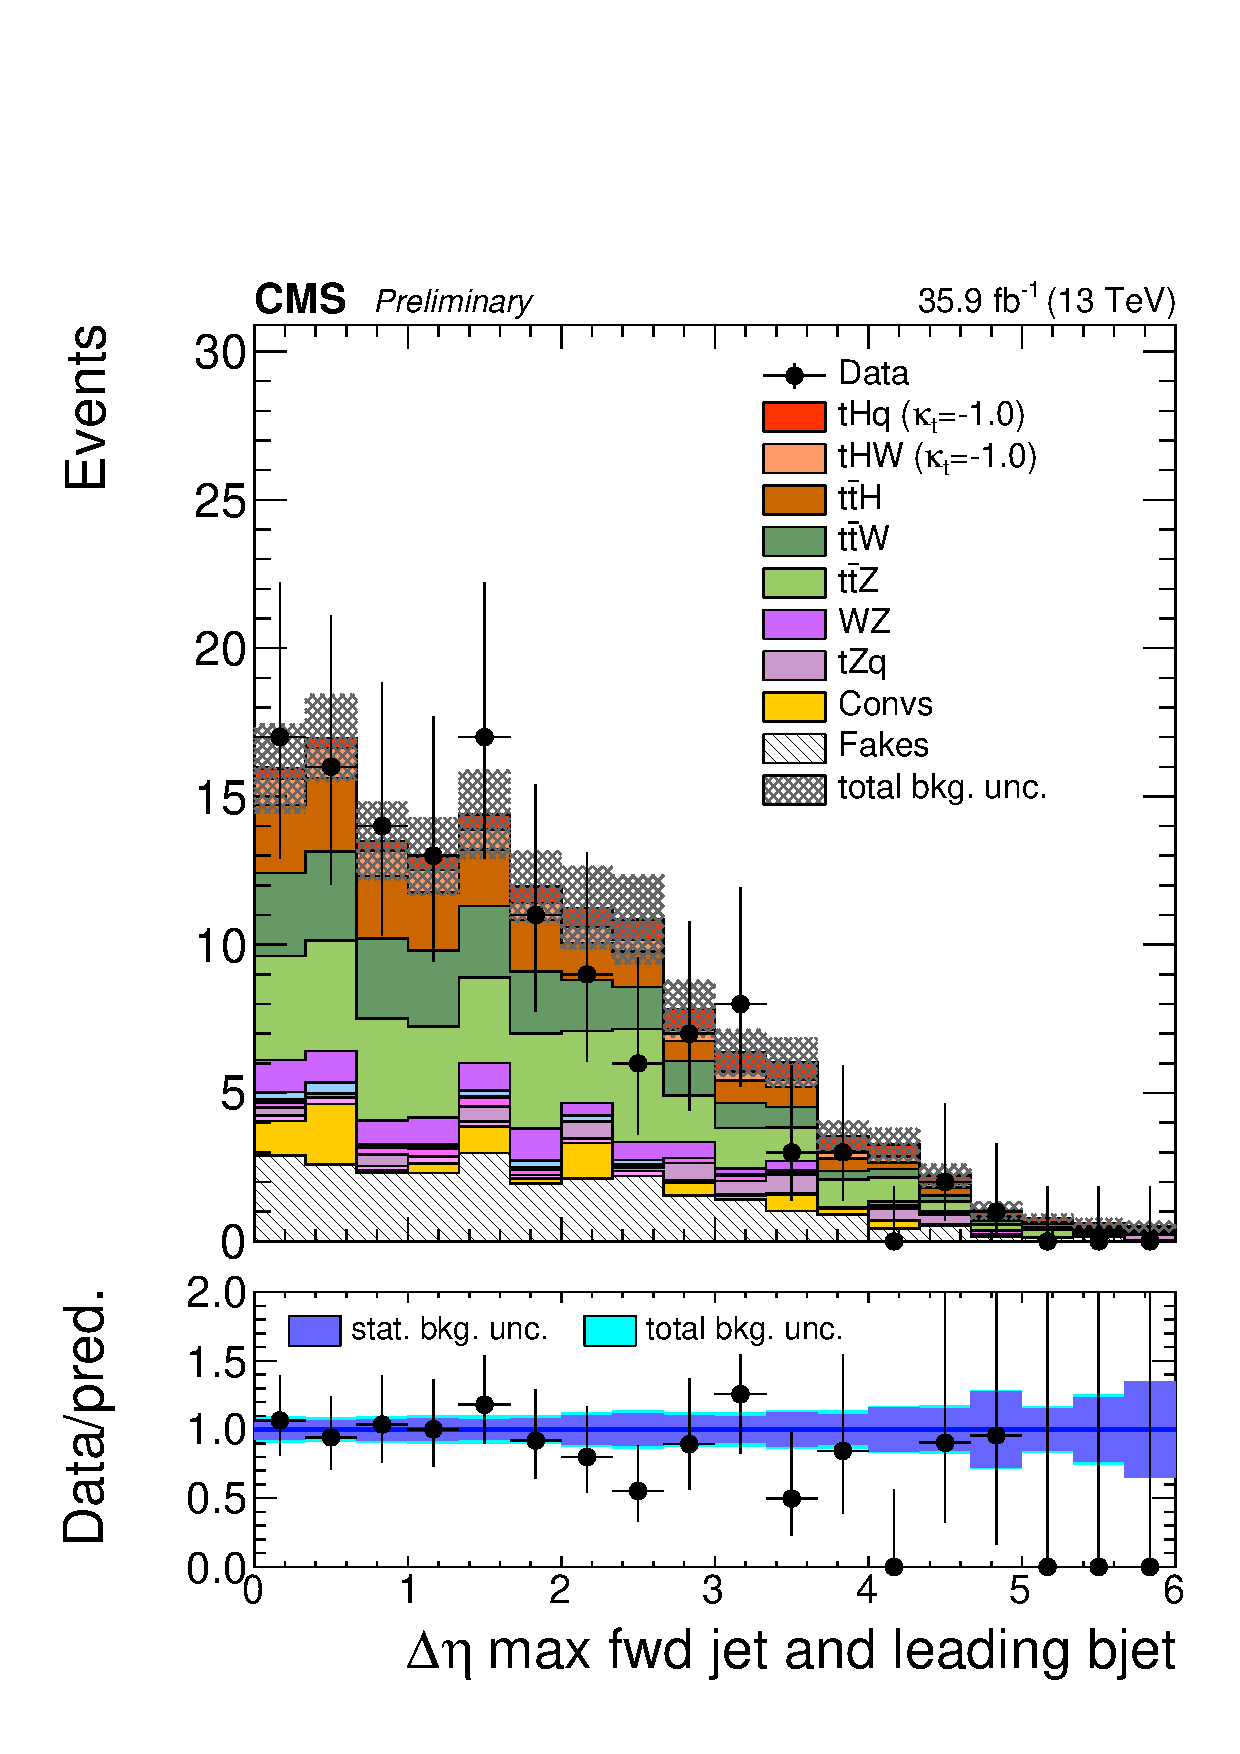
\includegraphics[width=0.22\textwidth]{figures/3lsignal/dEtaFwdJetBJet_40.pdf}
 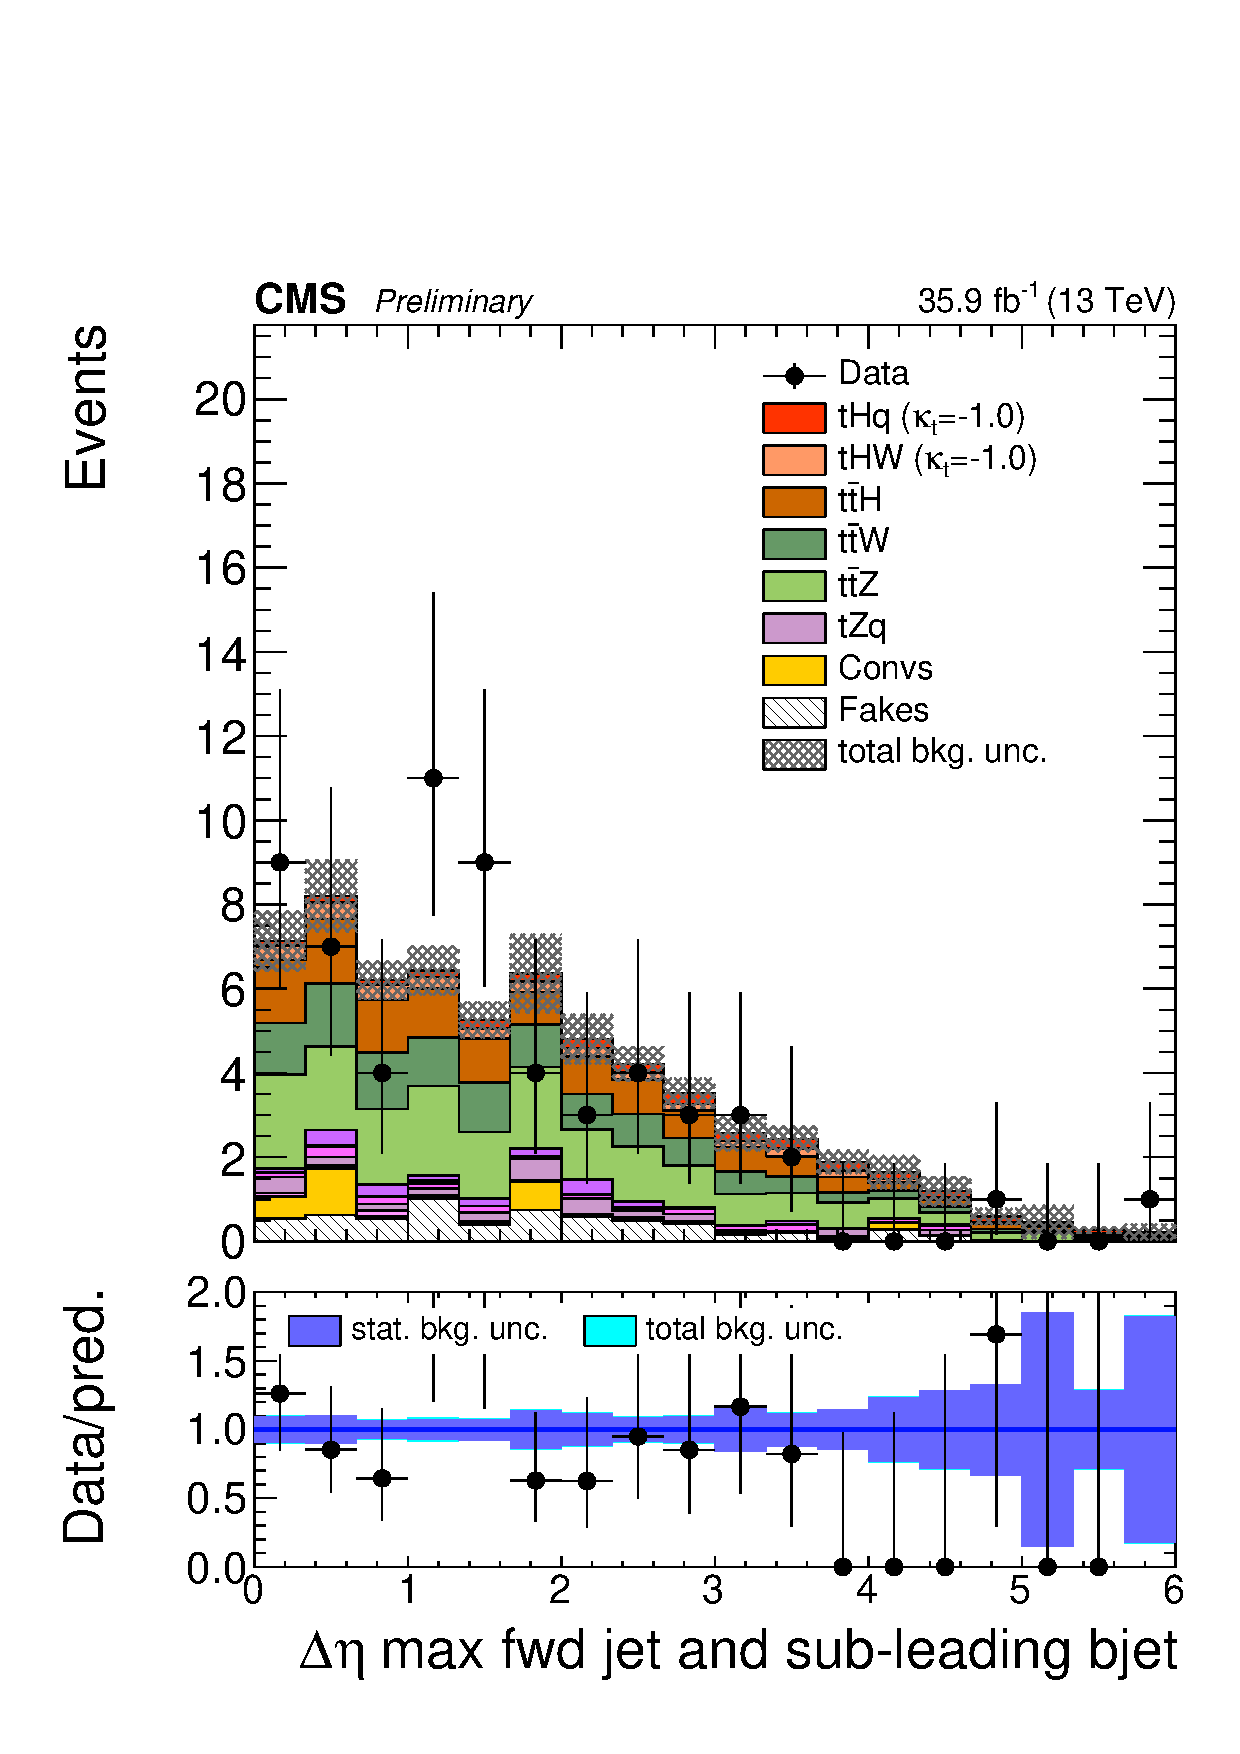
\includegraphics[width=0.22\textwidth]{figures/3lsignal/dEtaFwdJet2BJet_40.pdf}
 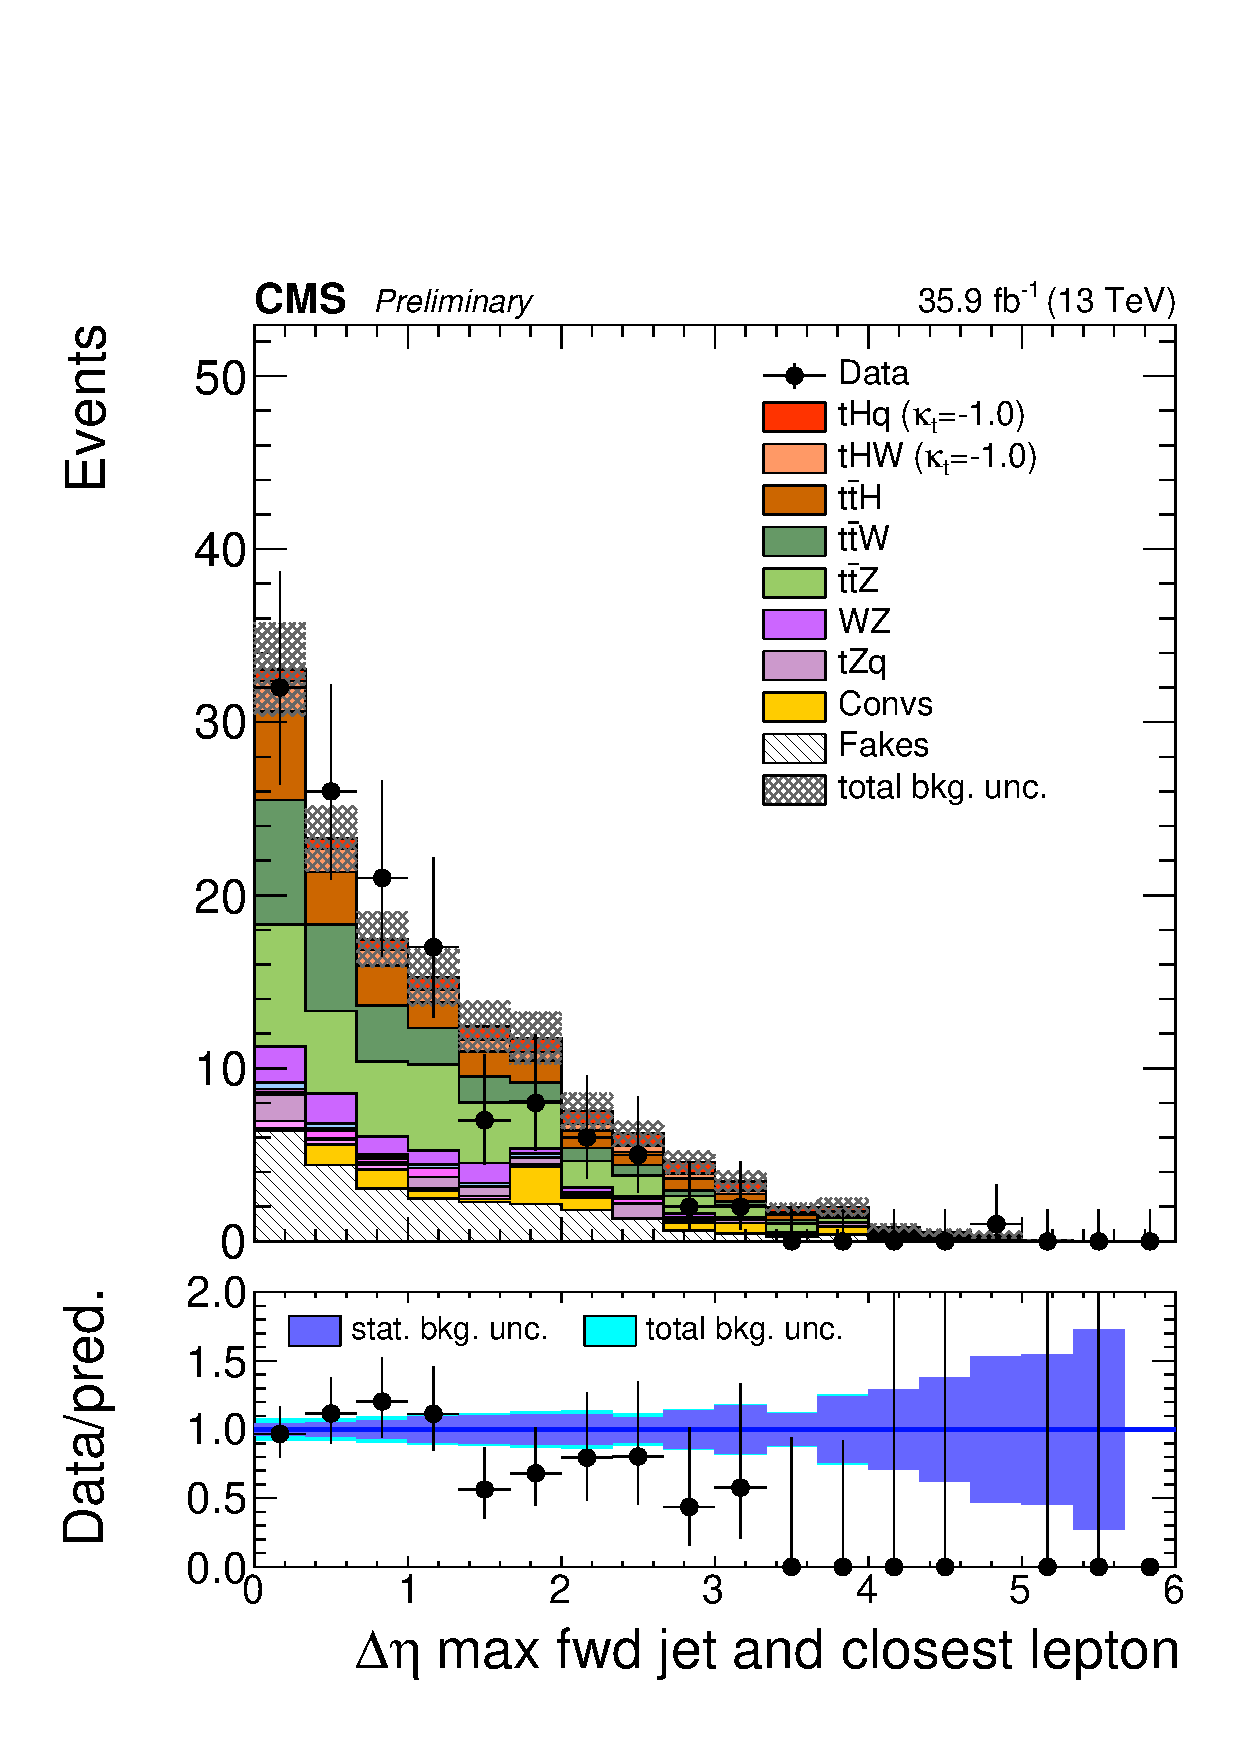
\includegraphics[width=0.22\textwidth]{figures/3lsignal/dEtaFwdJetClosestLep_40.pdf} \\
 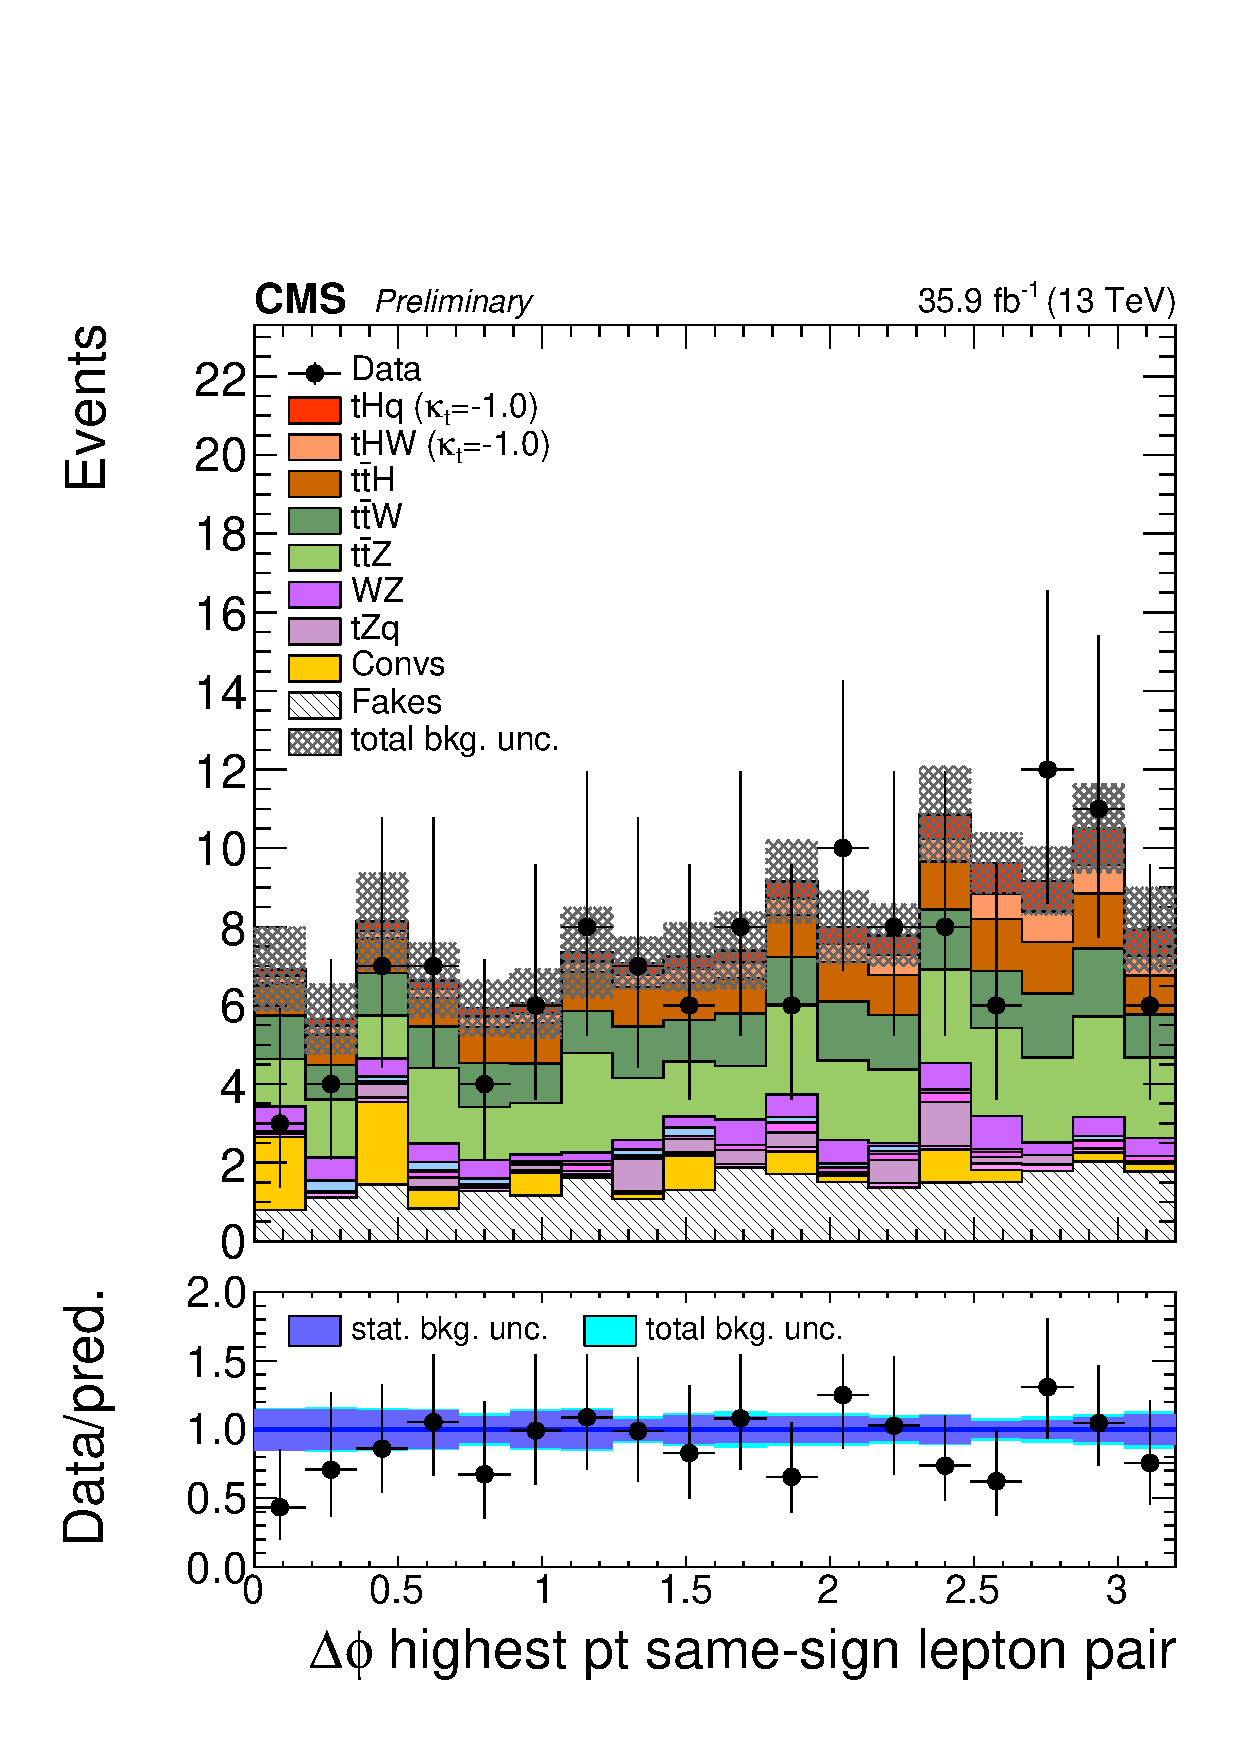
\includegraphics[width=0.22\textwidth]{figures/3lsignal/dPhiHighestPtSSPair.pdf}
 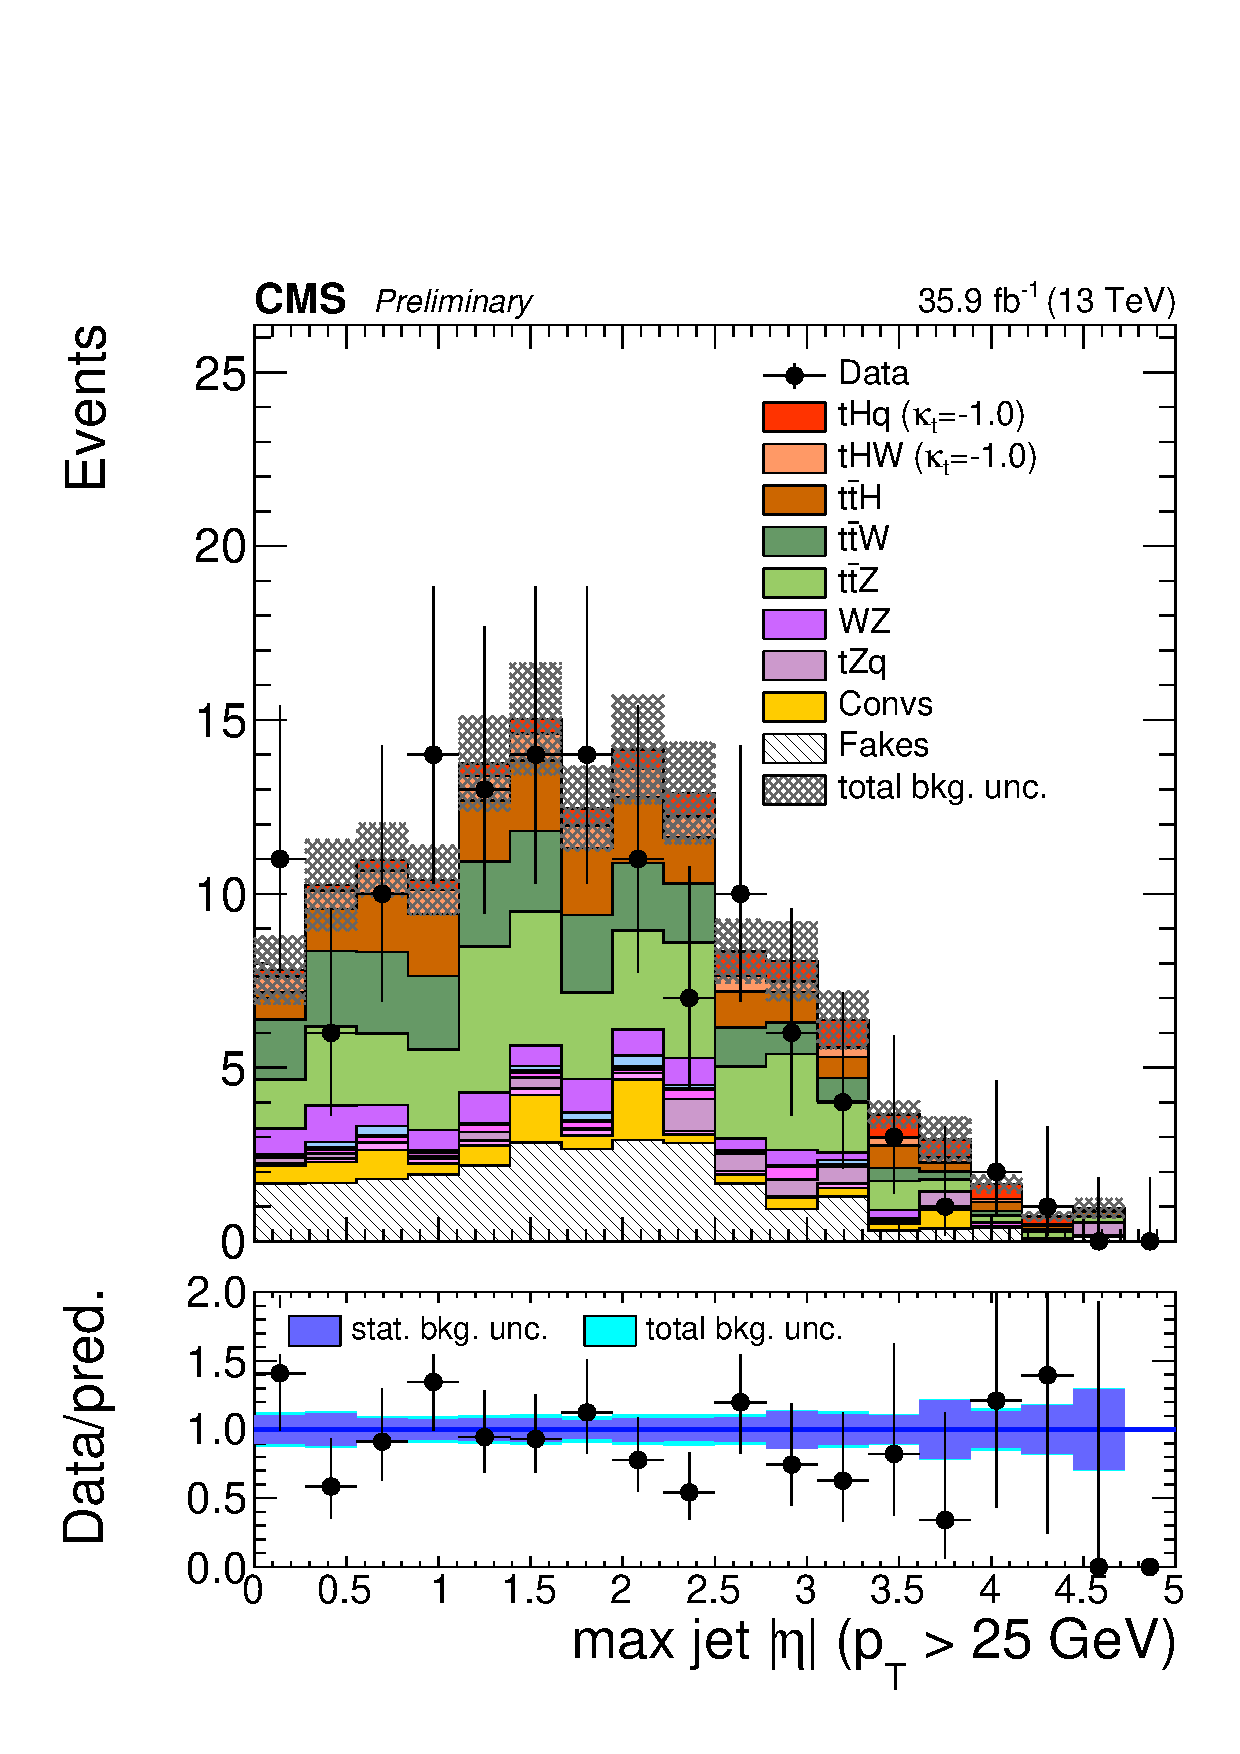
\includegraphics[width=0.22\textwidth]{figures/3lsignal/maxEtaJet25_40.pdf}
 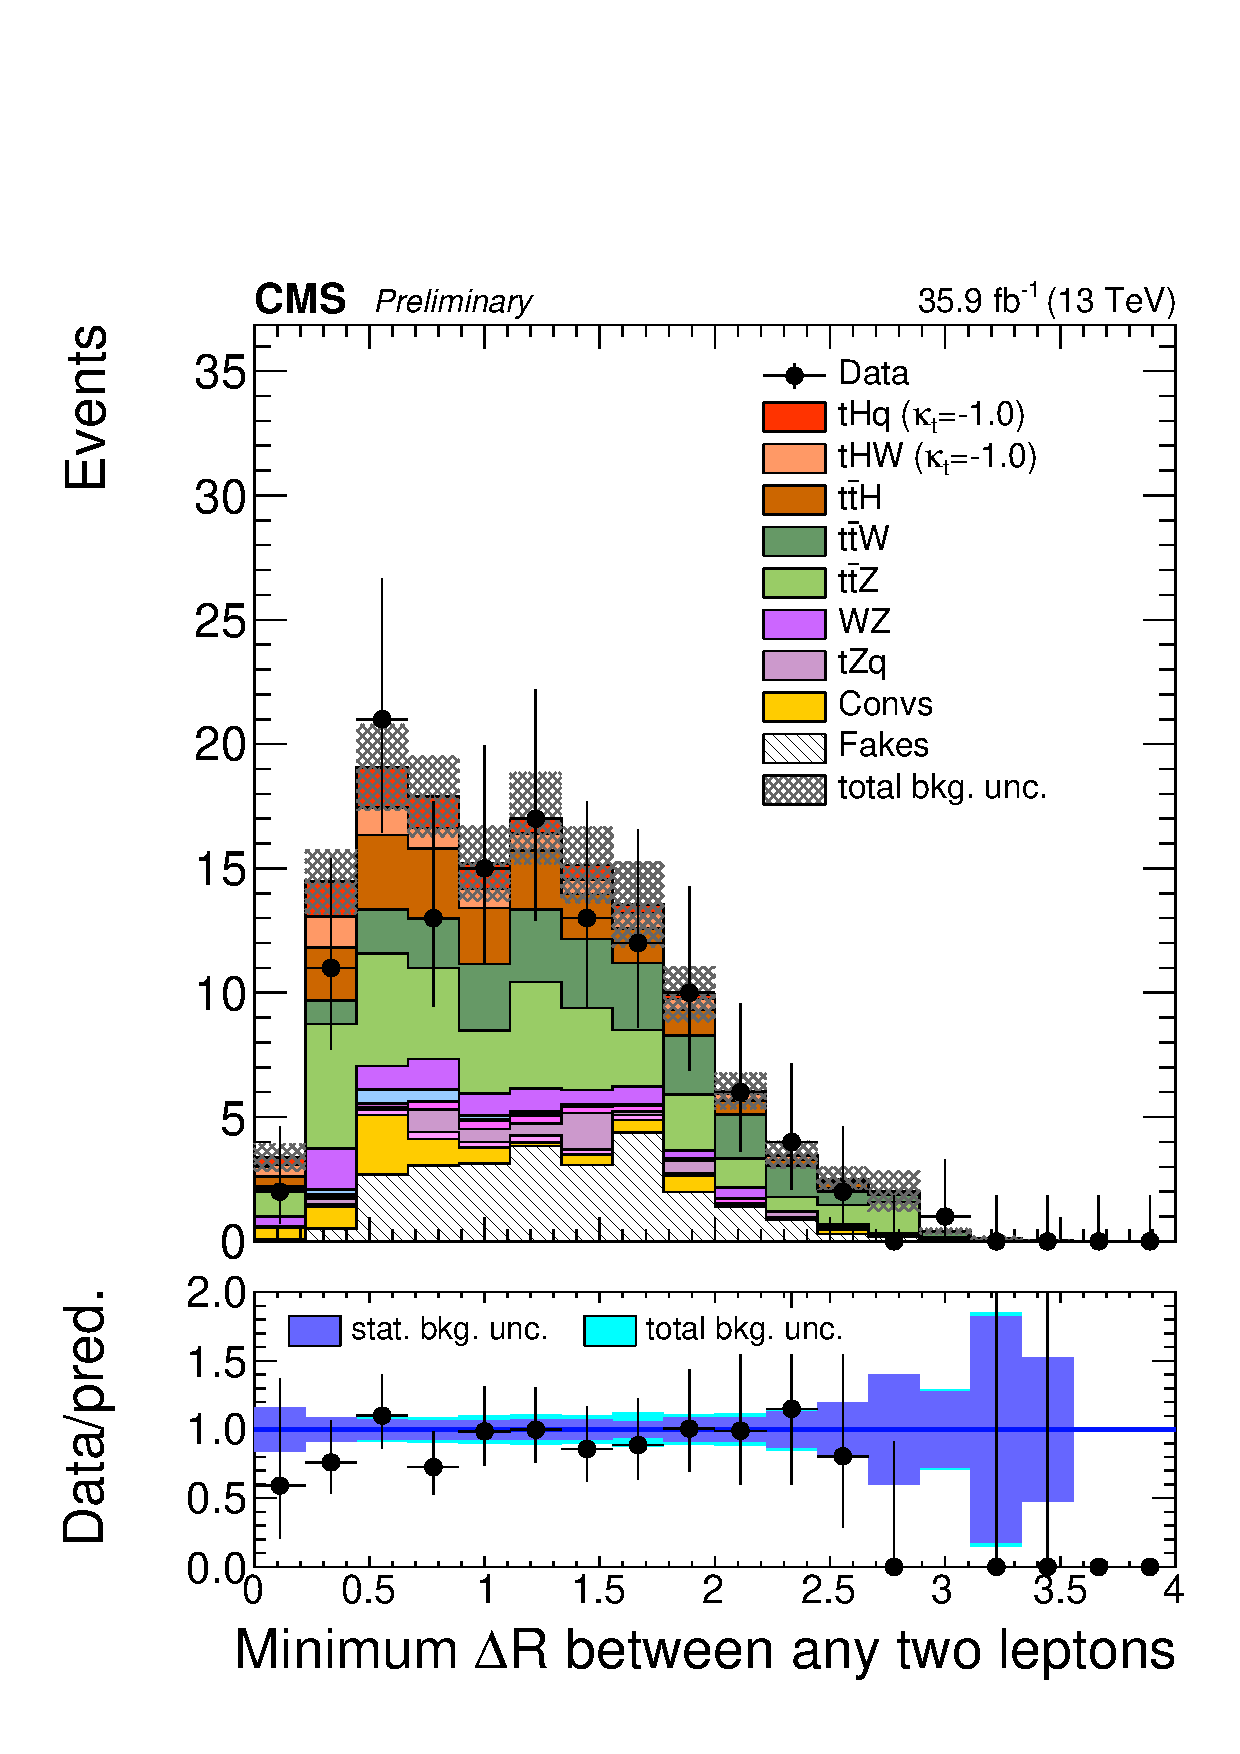
\includegraphics[width=0.22\textwidth]{figures/3lsignal/minDRll.pdf}
 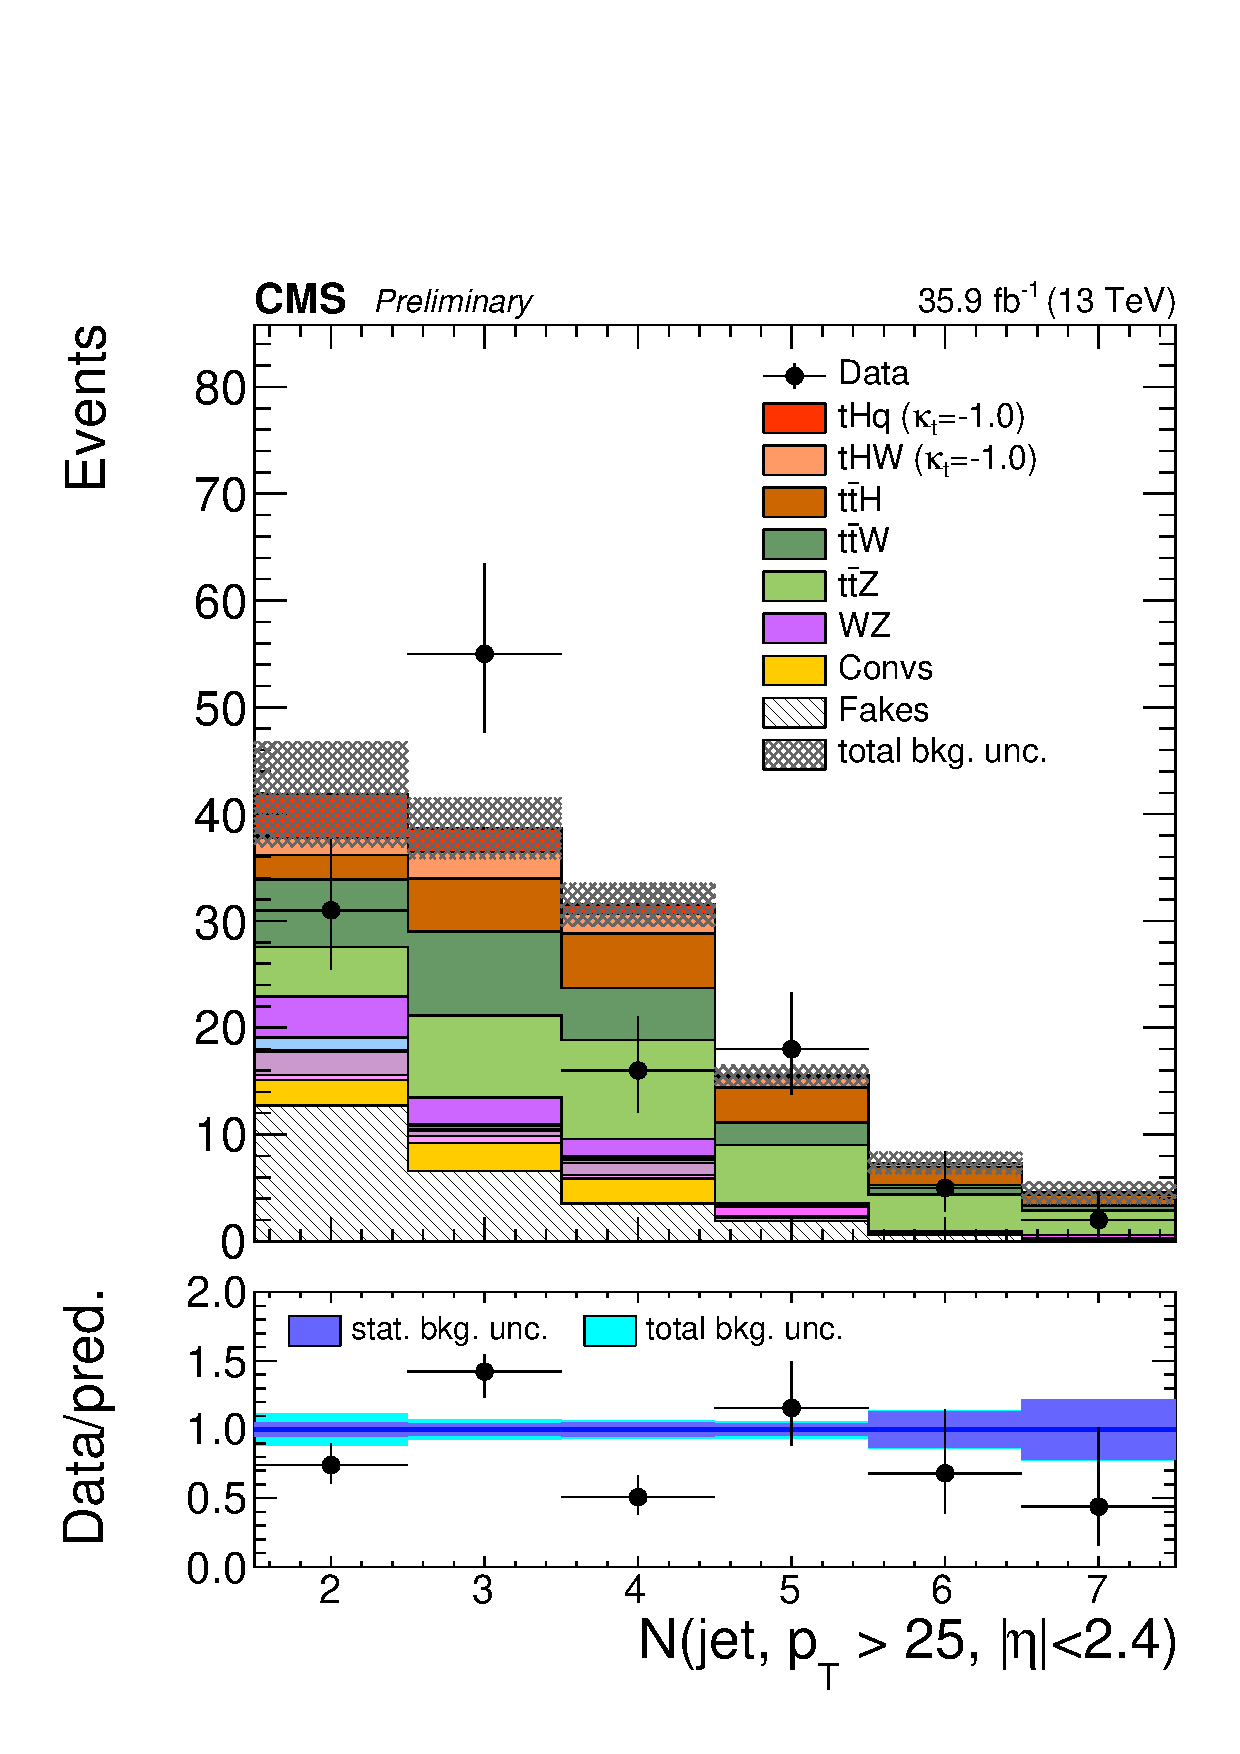
\includegraphics[width=0.22\textwidth]{figures/3lsignal/nJet25.pdf} \\
 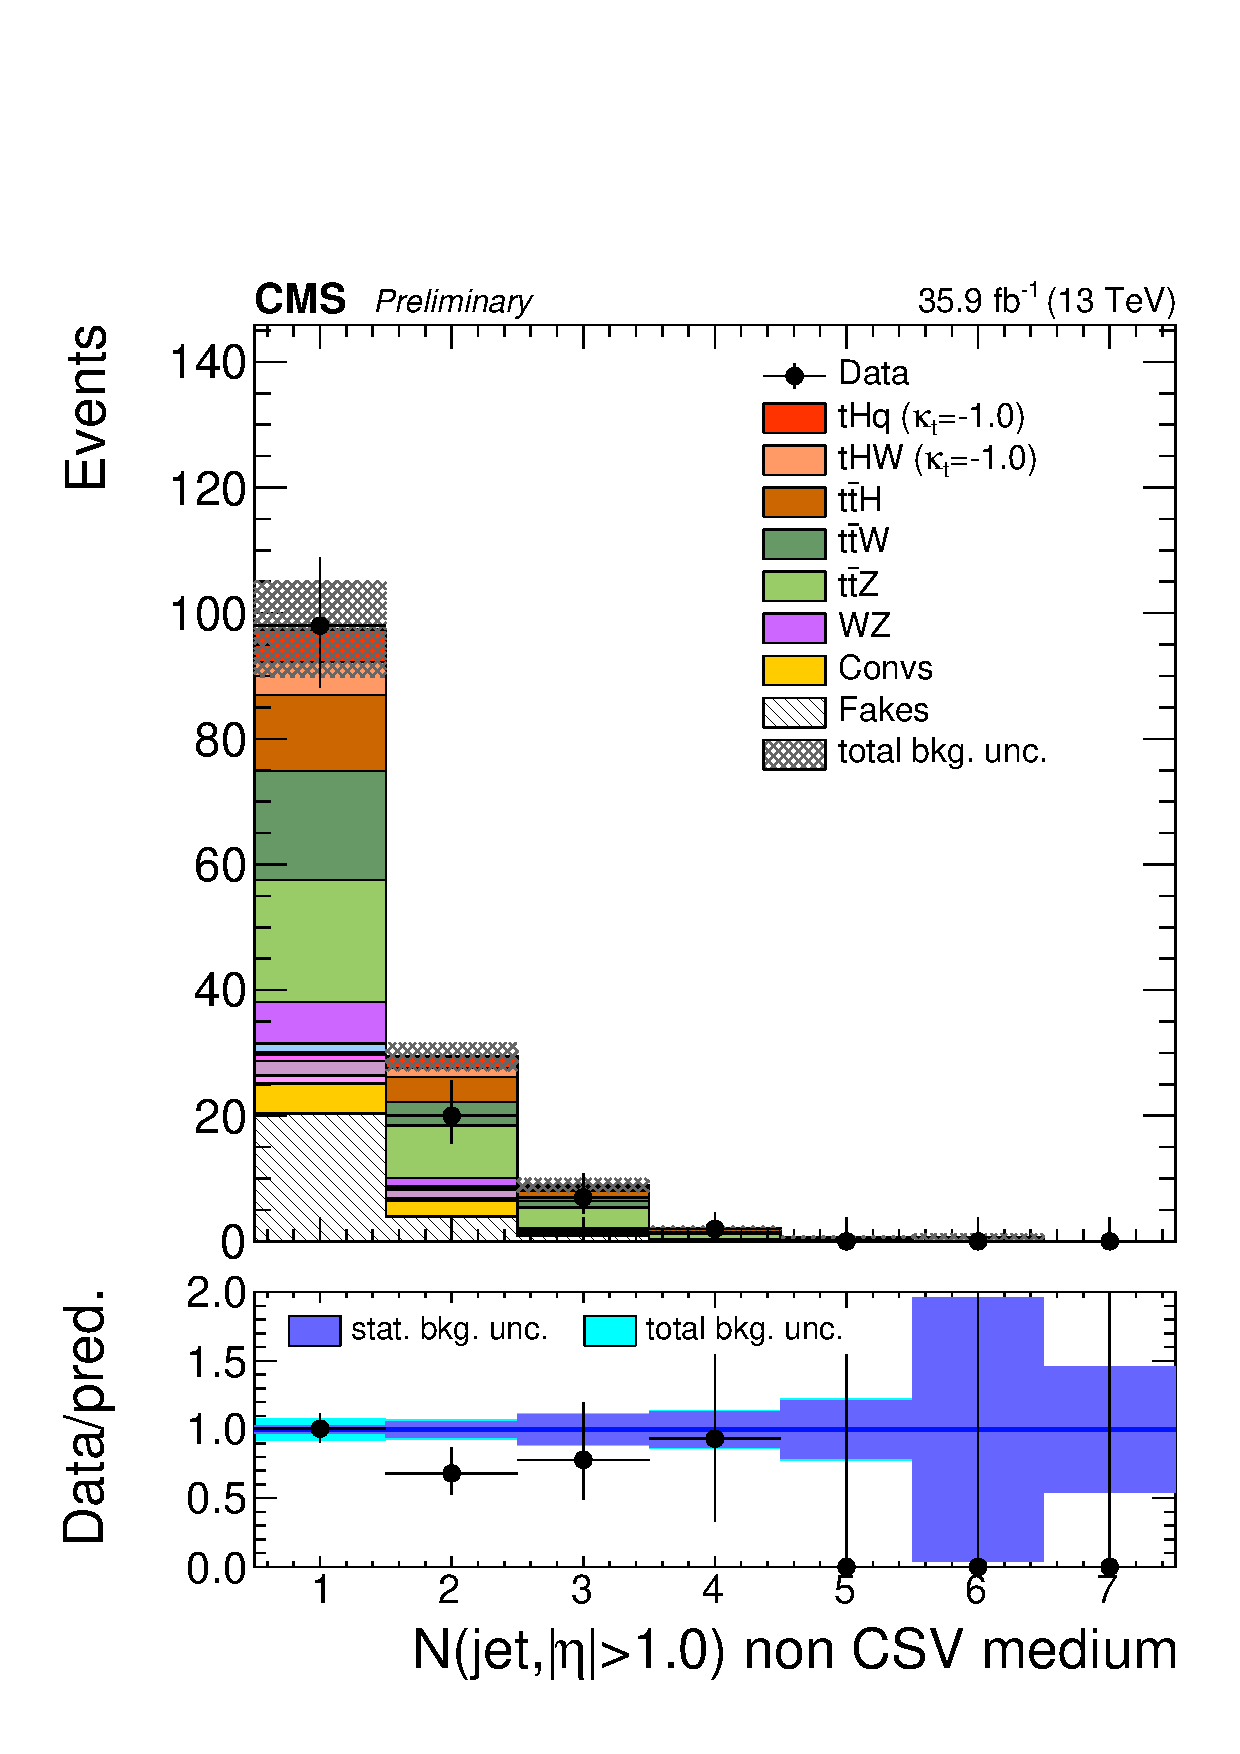
\includegraphics[width=0.22\textwidth]{figures/3lsignal/nJetEta1_40.pdf}
 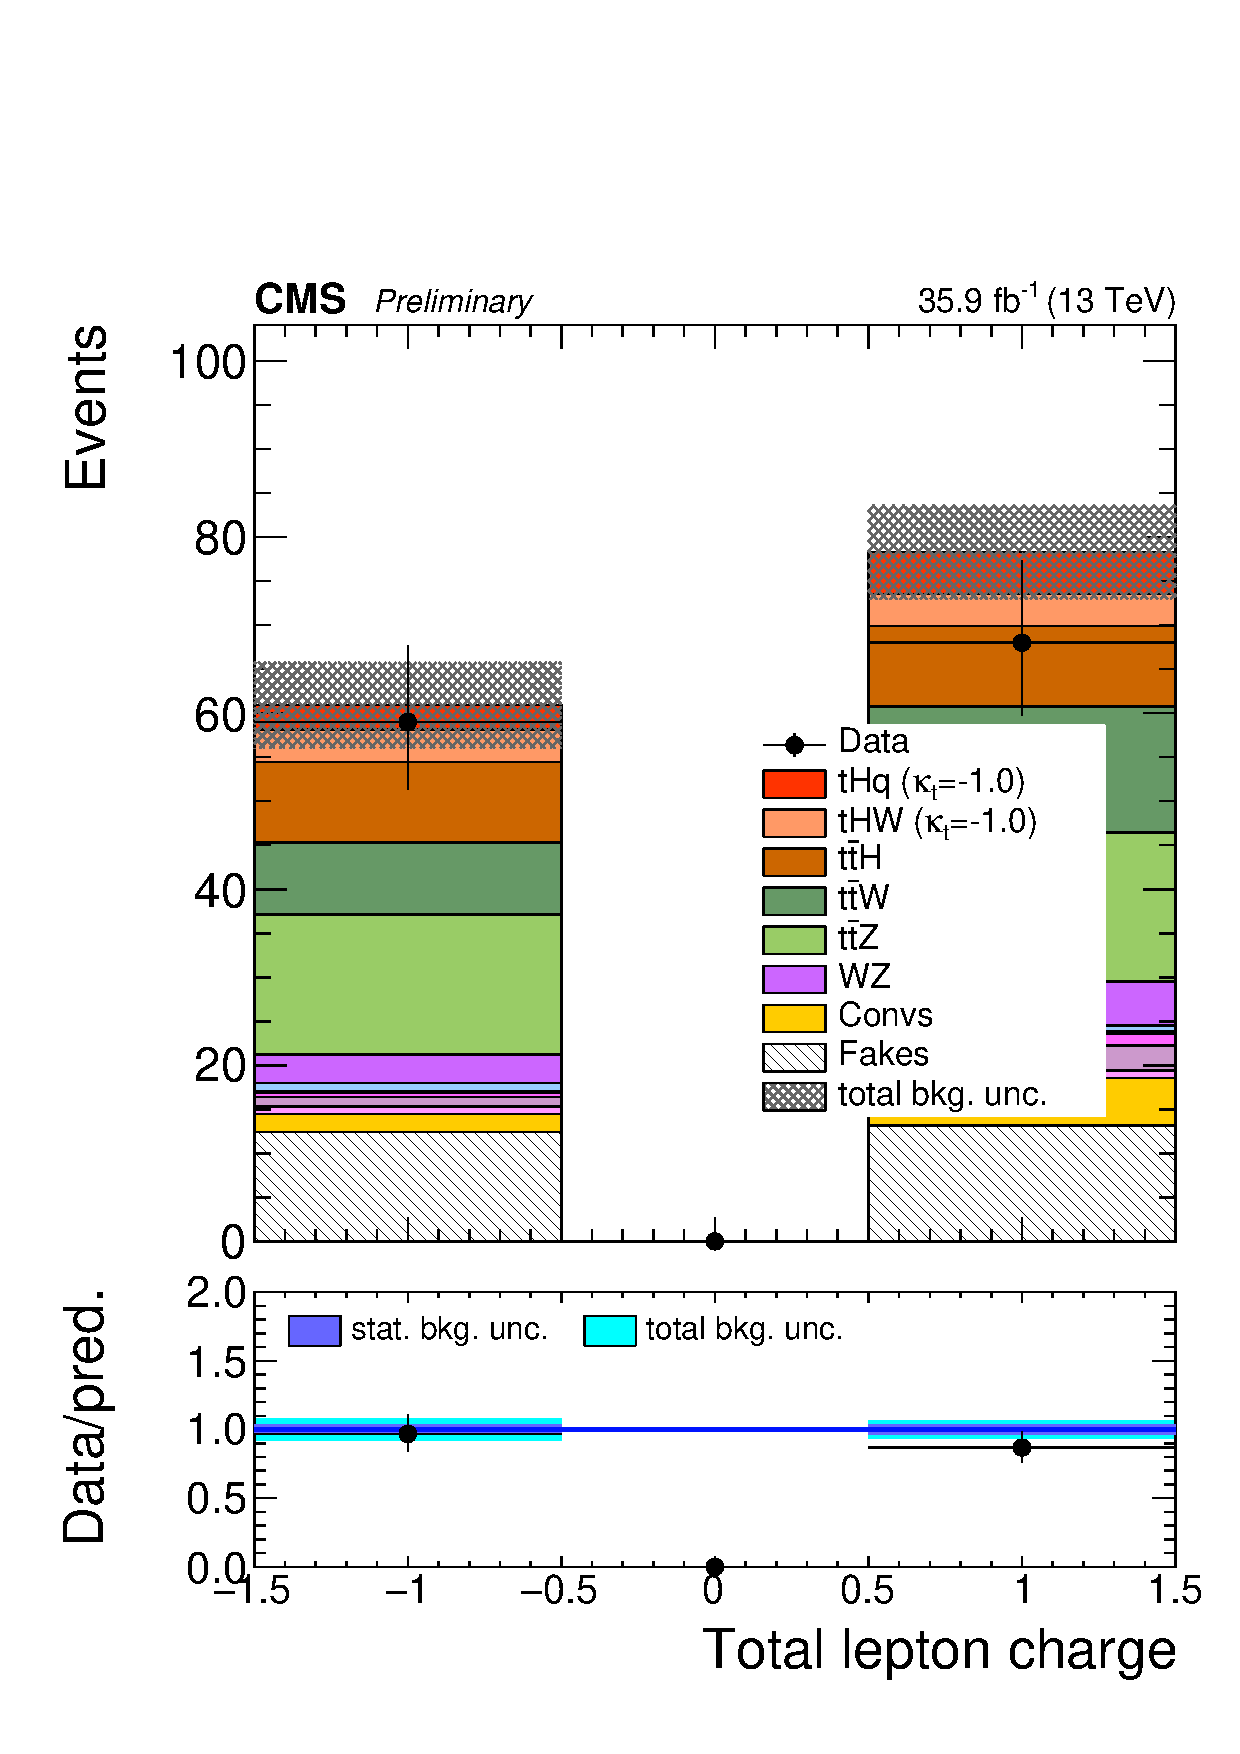
\includegraphics[width=0.22\textwidth]{figures/3lsignal/totCharge.pdf}
\caption{Distributions of input variables to the BDT for signal discrimination, three lepton channel, normalized to their cross section and to 35.9\fbinv.} 
\label{fig:input_vars_3l_xsec}
\end{figure}    

\begin{figure} [!h]
  \centering
  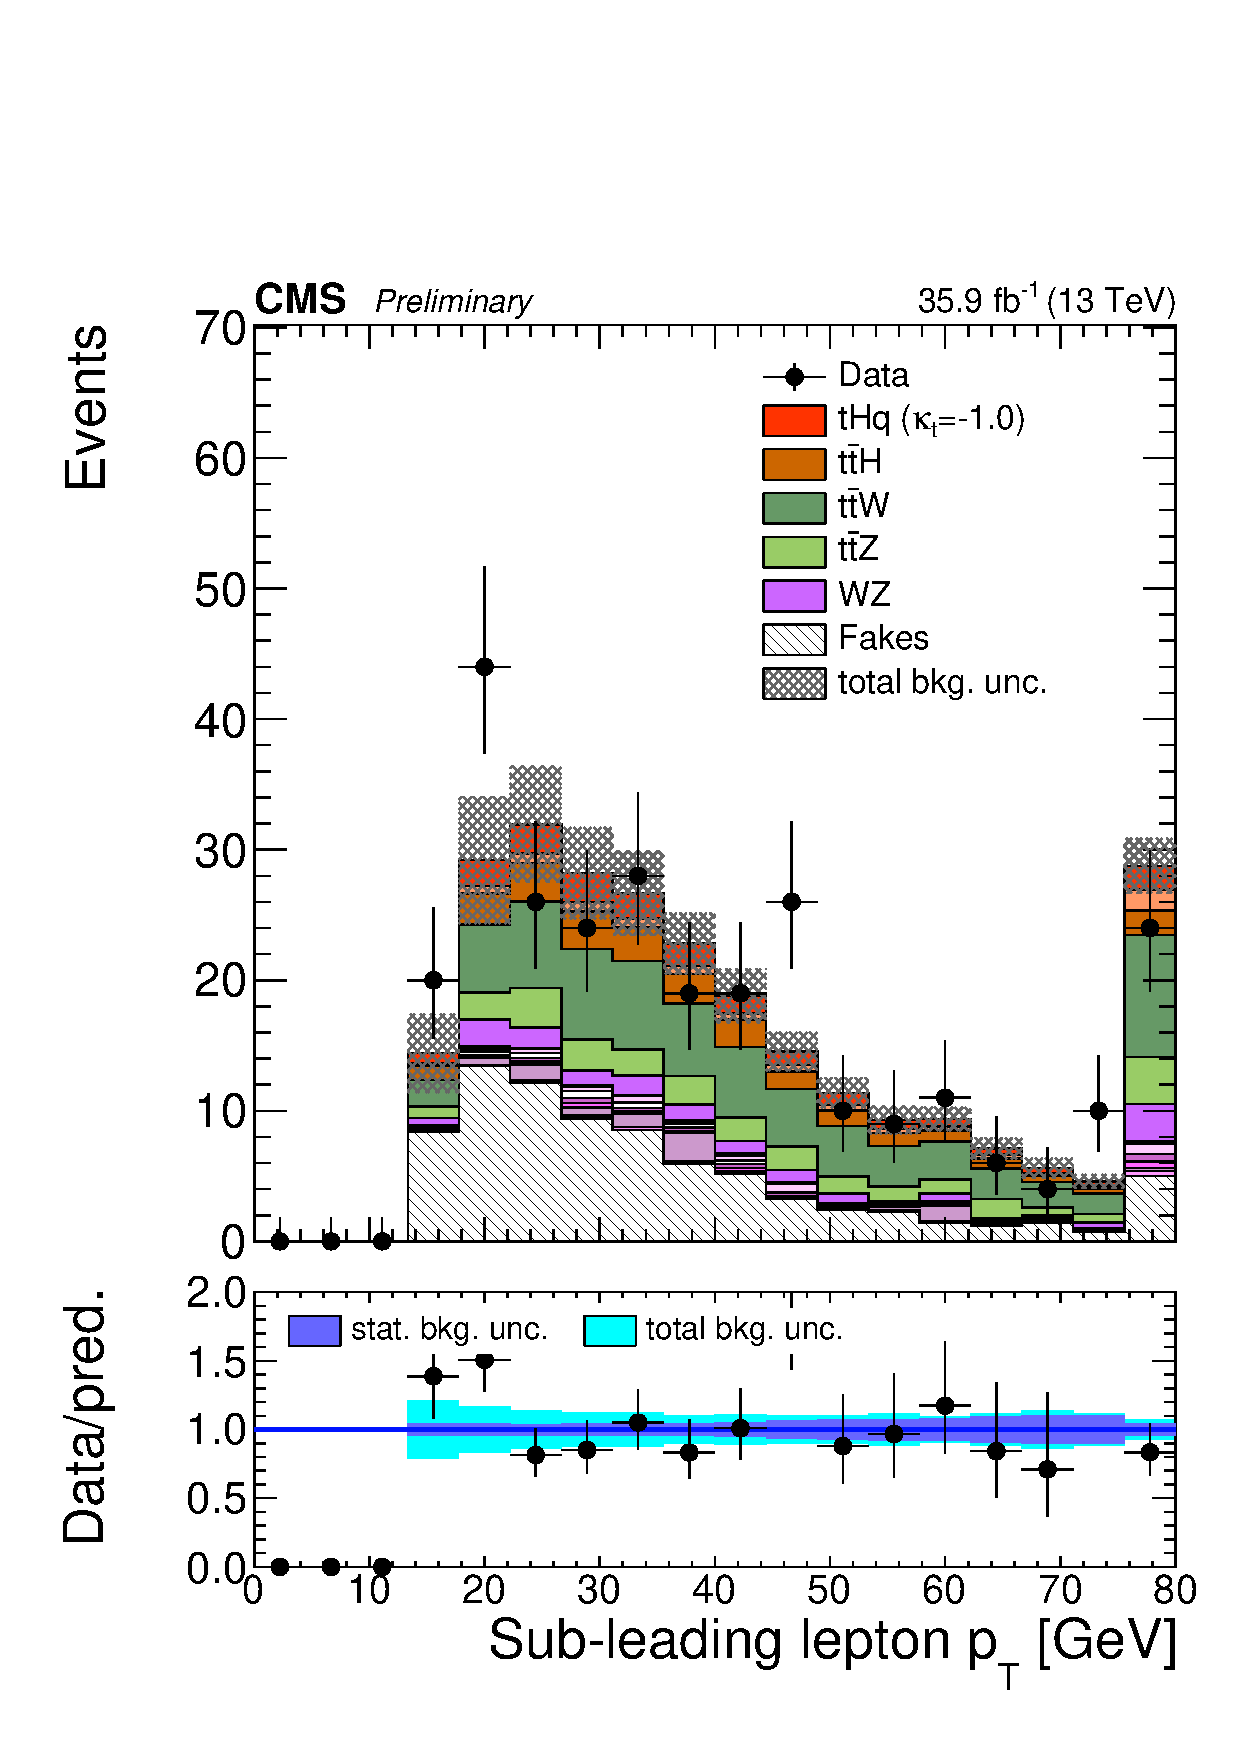
\includegraphics[width=0.22\textwidth]{figures/signalregion_2lss/mumu/Lep2Pt.pdf}
  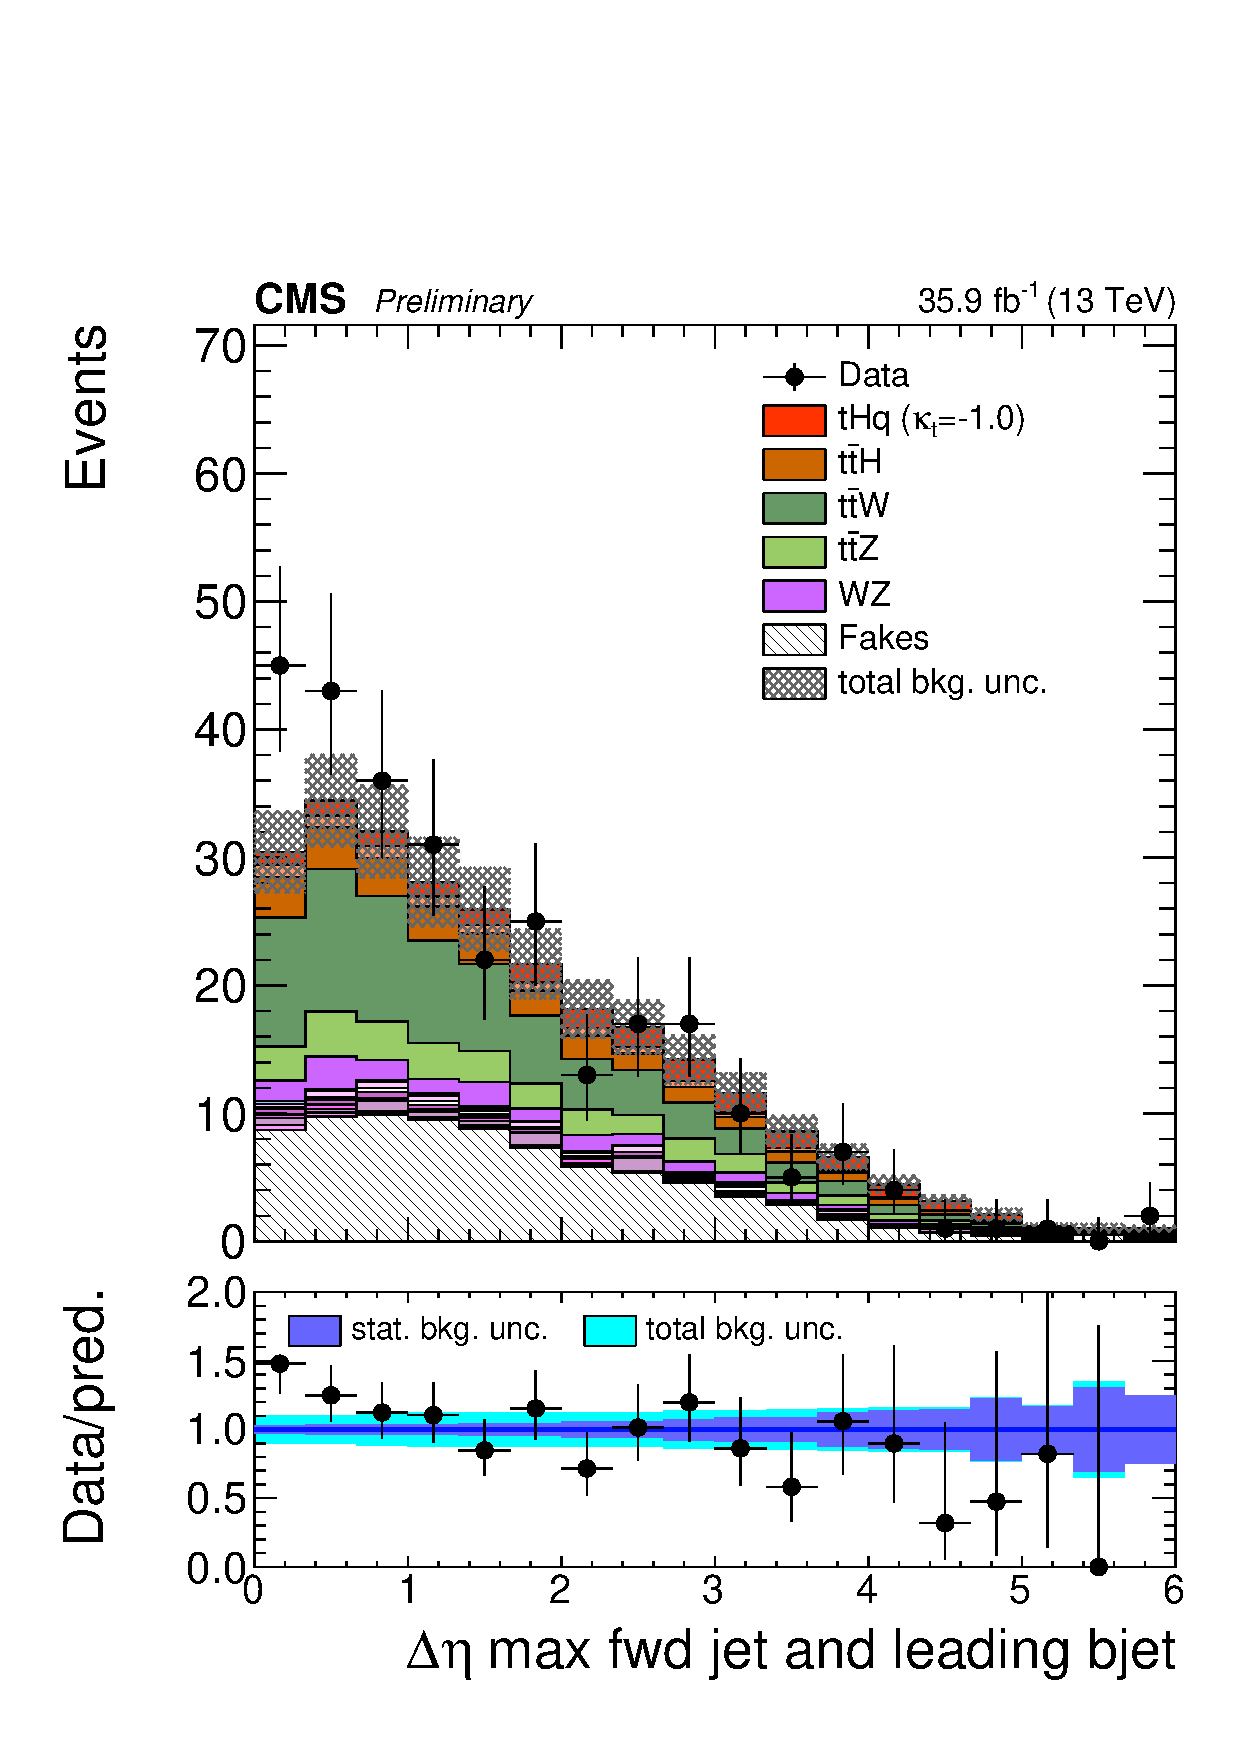
\includegraphics[width=0.22\textwidth]{figures/signalregion_2lss/mumu/dEtaFwdJetBJet_40.pdf}
  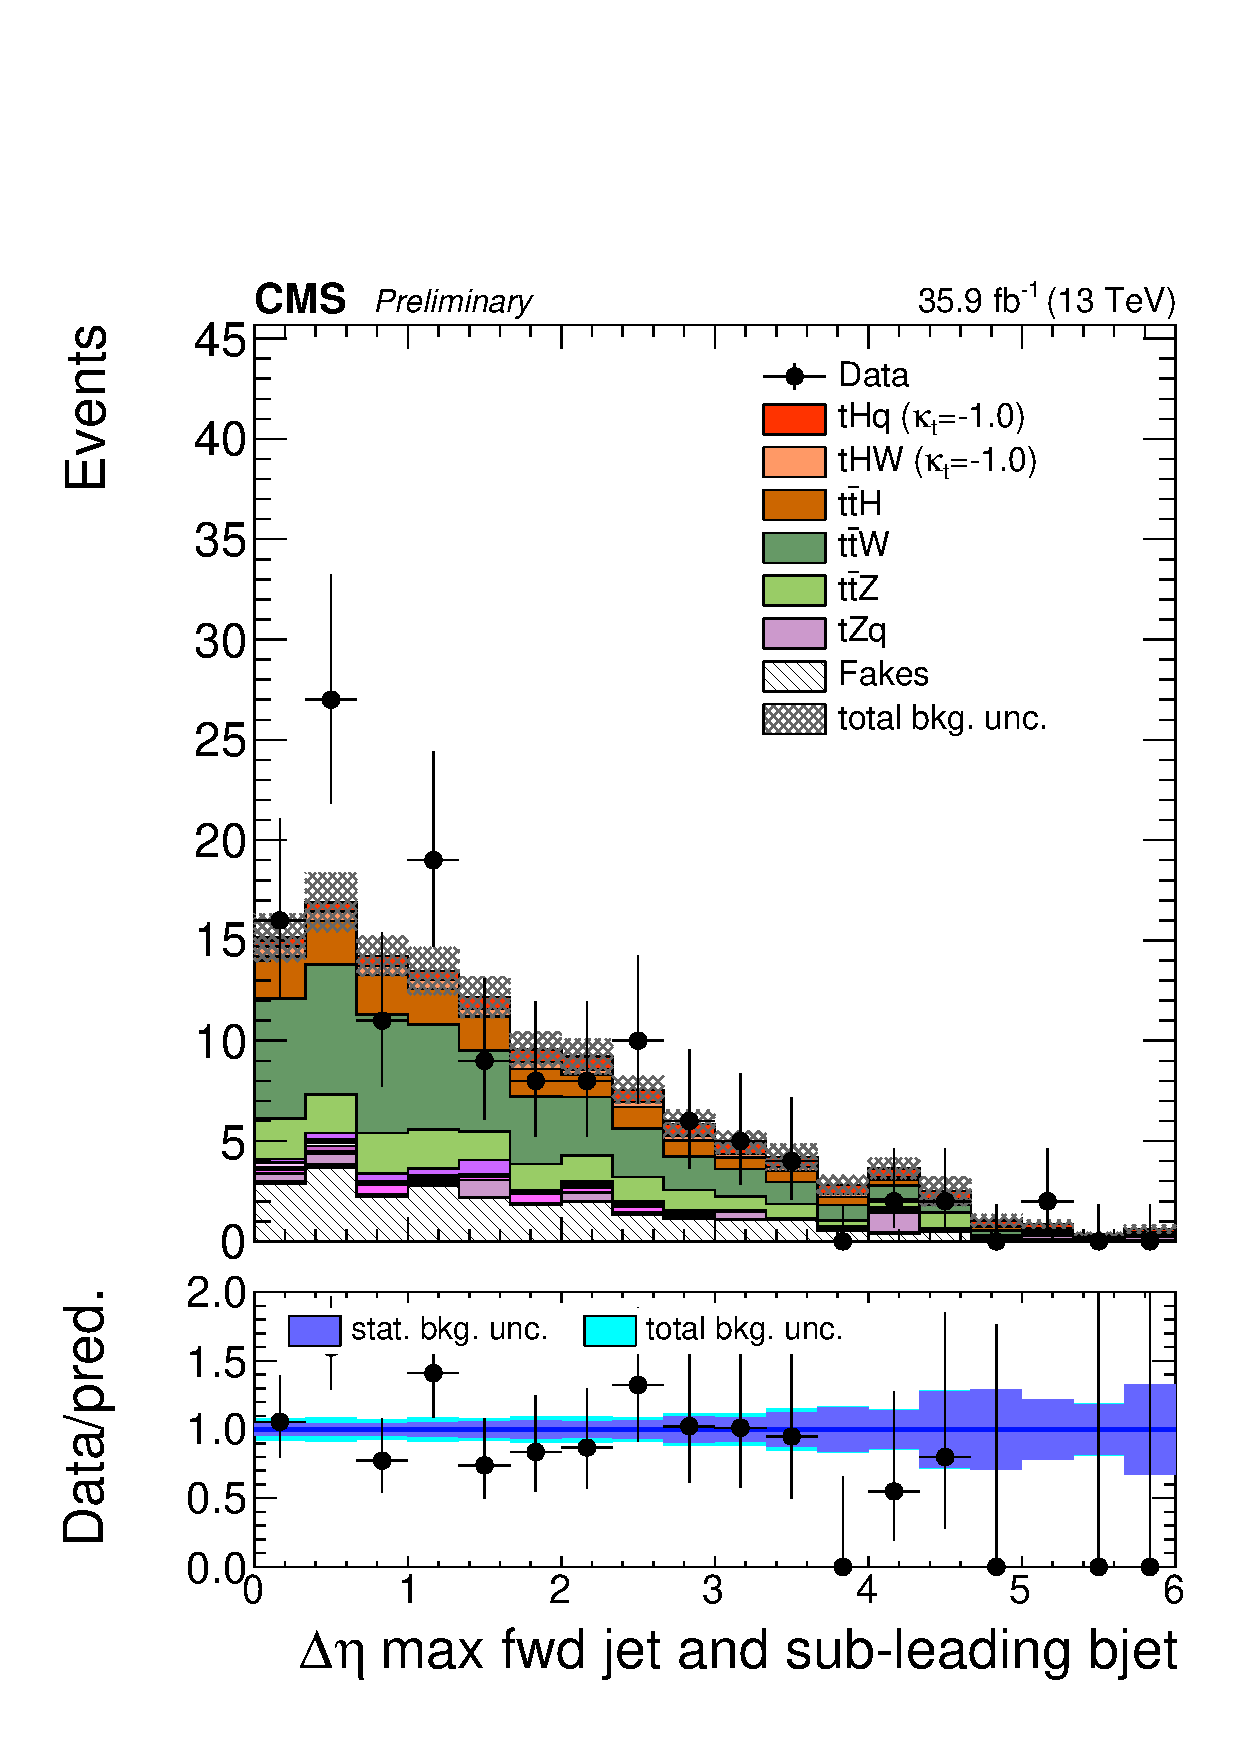
\includegraphics[width=0.22\textwidth]{figures/signalregion_2lss/mumu/dEtaFwdJet2BJet_40.pdf}
  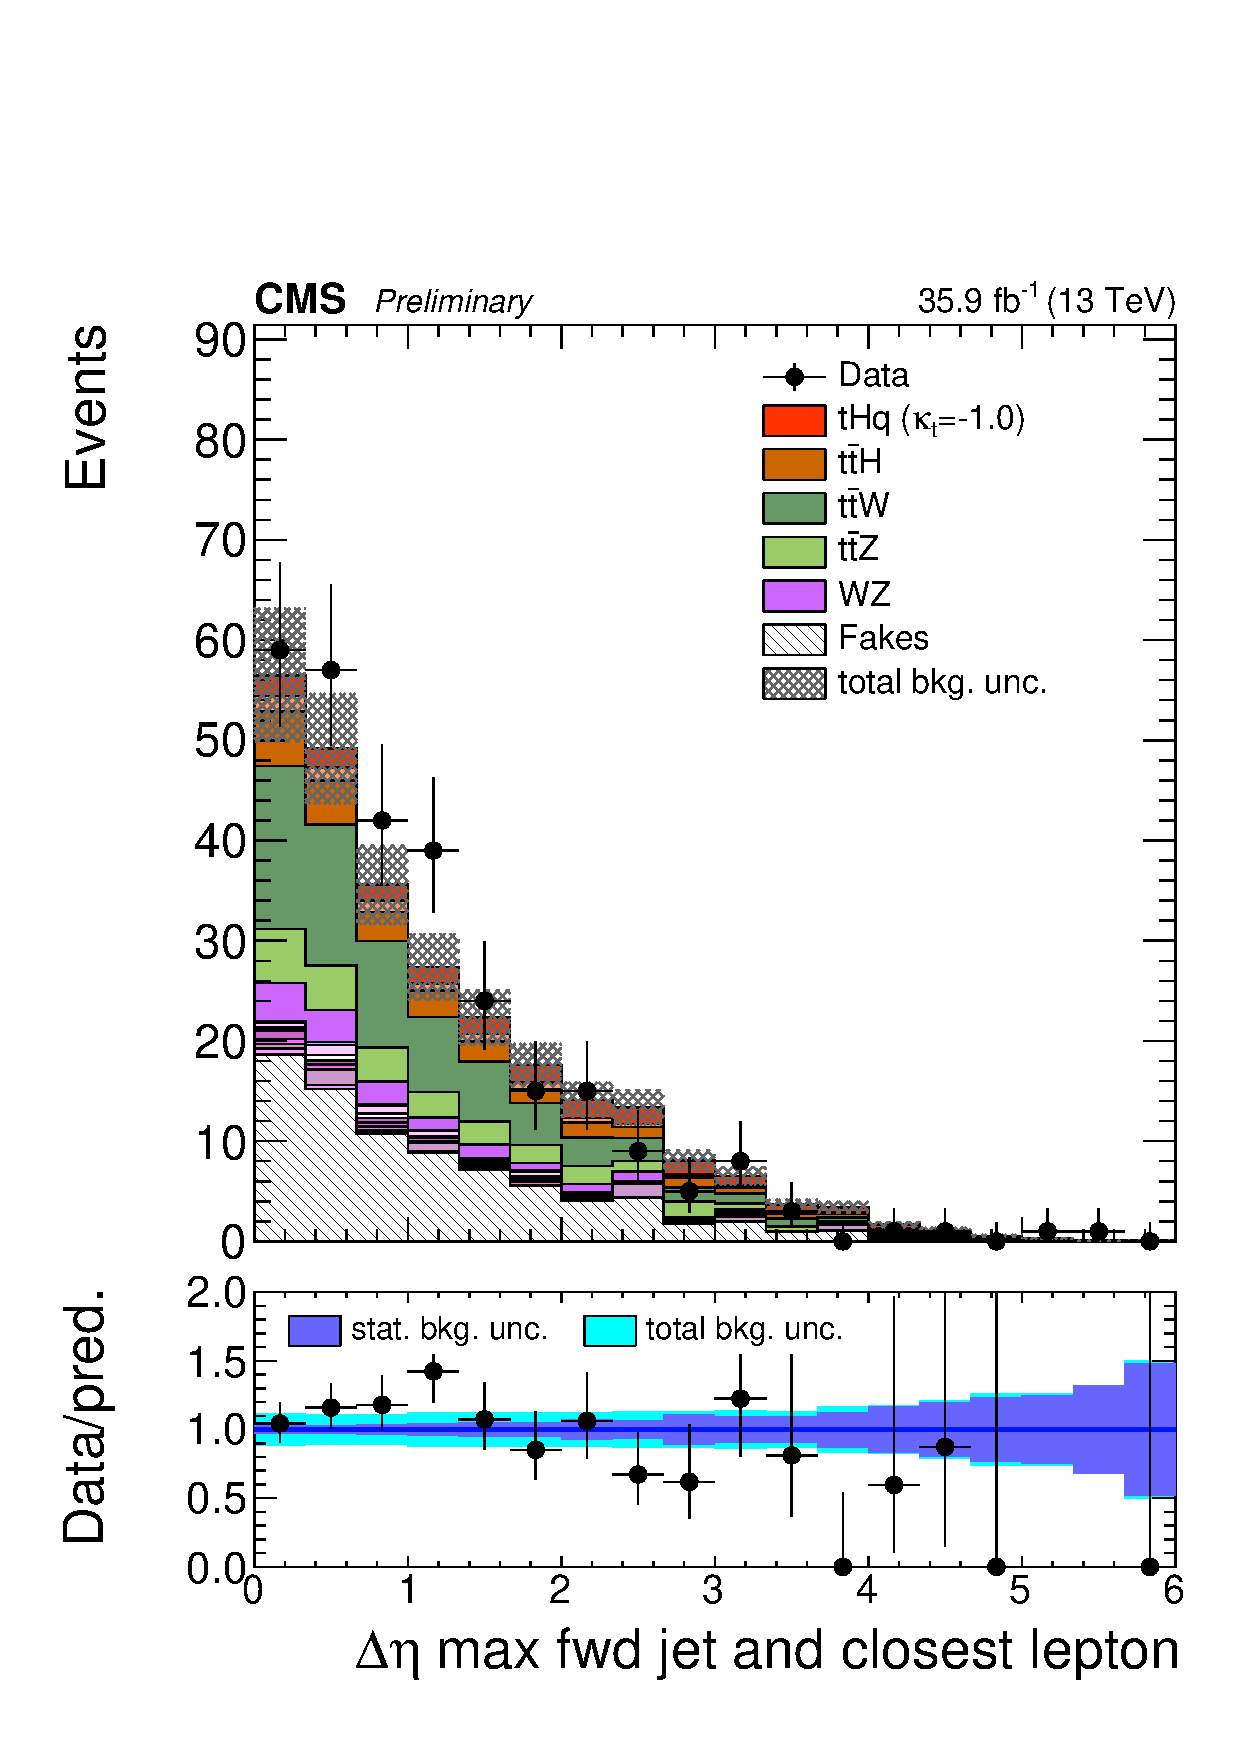
\includegraphics[width=0.22\textwidth]{figures/signalregion_2lss/mumu/dEtaFwdJetClosestLep_40.pdf} \\
  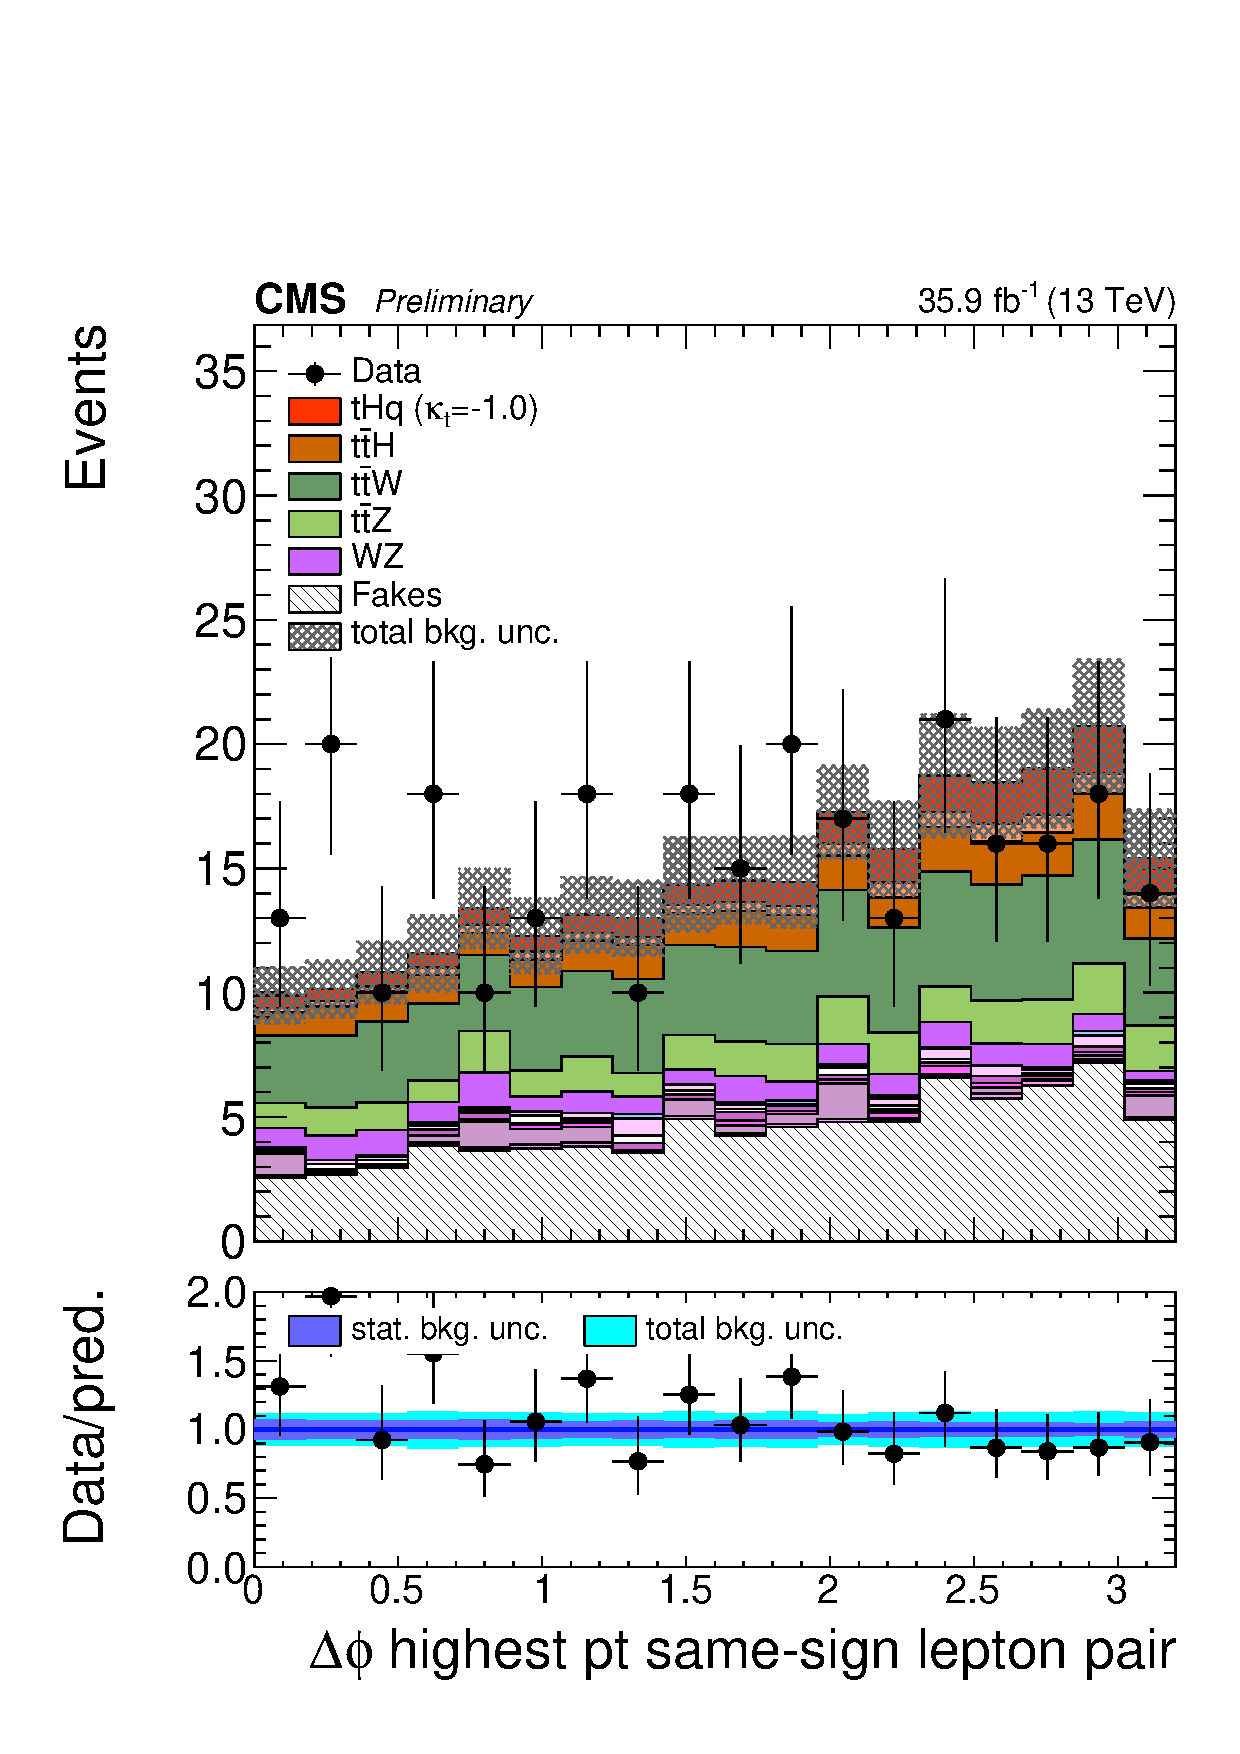
\includegraphics[width=0.22\textwidth]{figures/signalregion_2lss/mumu/dPhiHighestPtSSPair.pdf}
  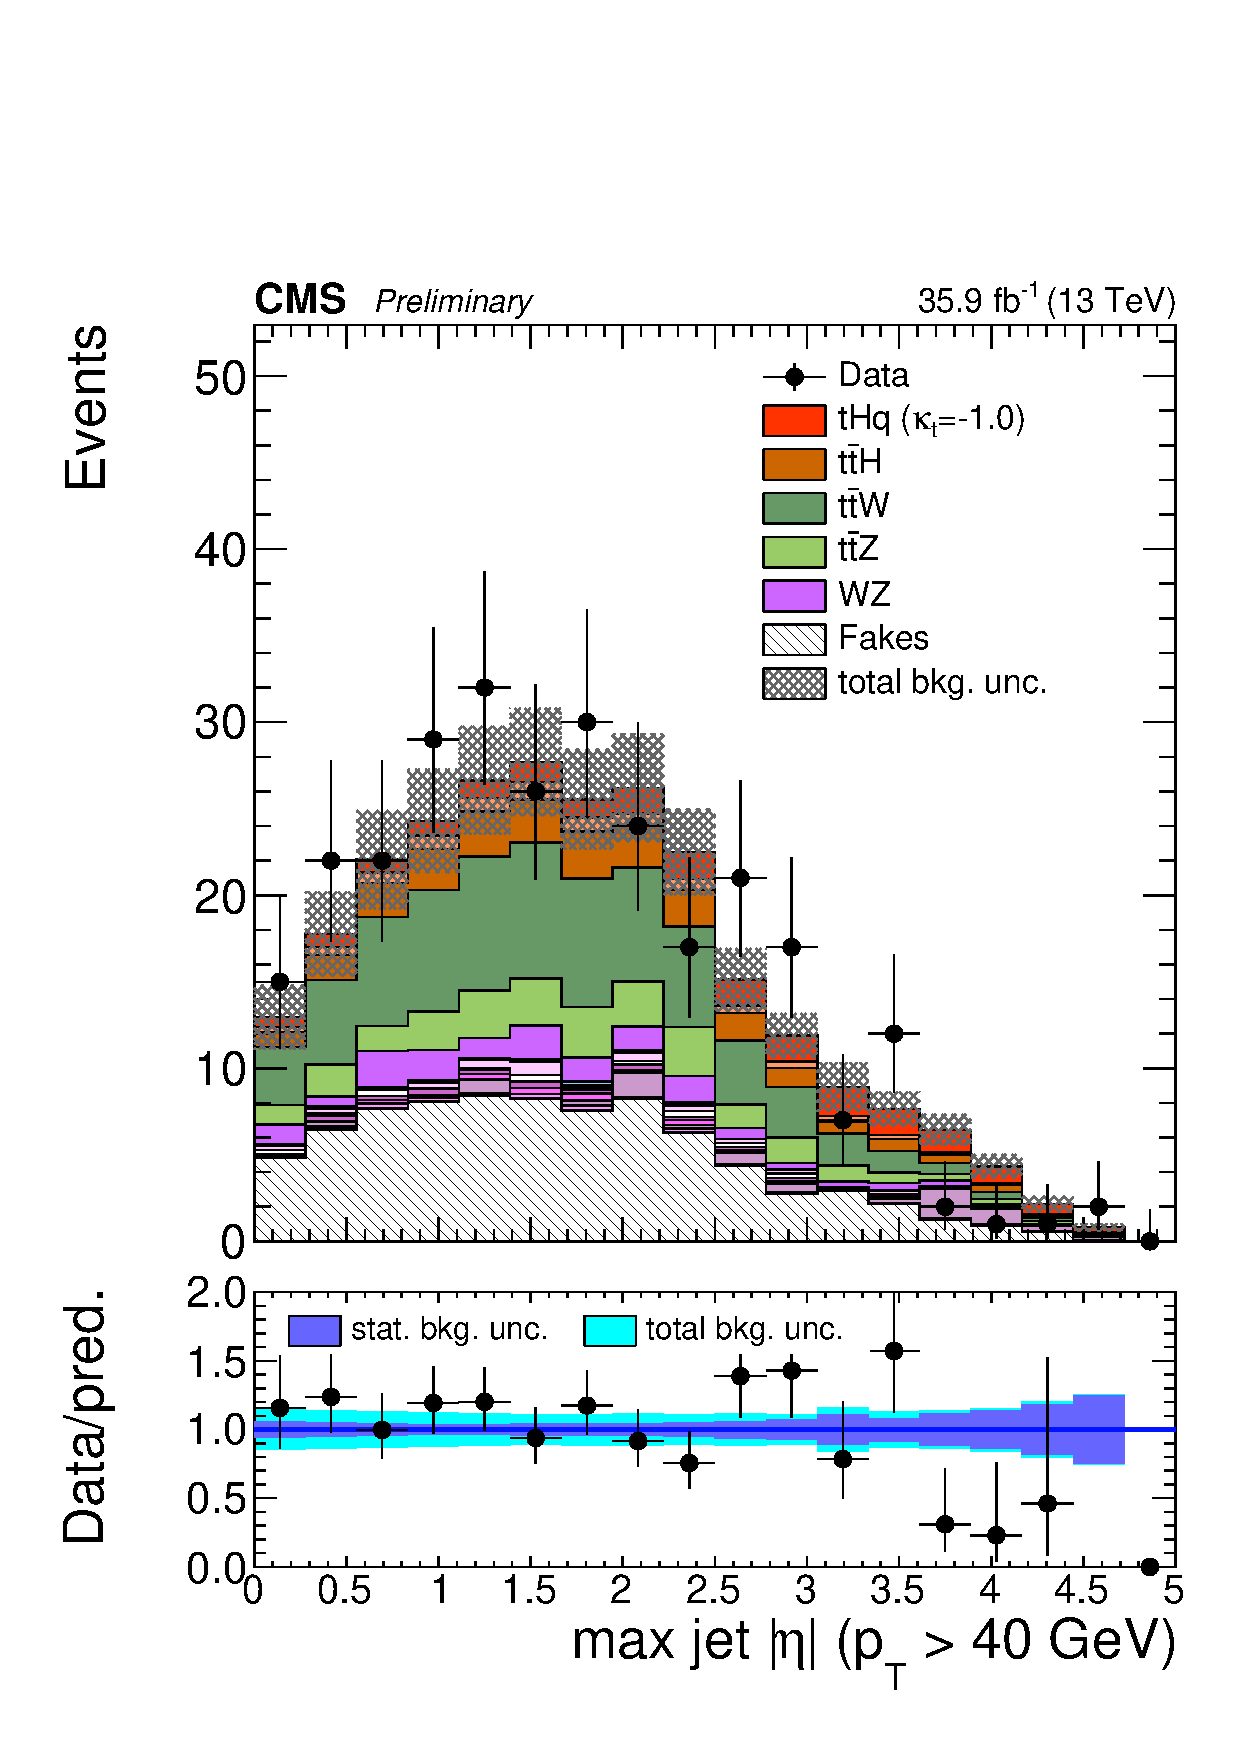
\includegraphics[width=0.22\textwidth]{figures/signalregion_2lss/mumu/maxEtaJet25_40.pdf}
  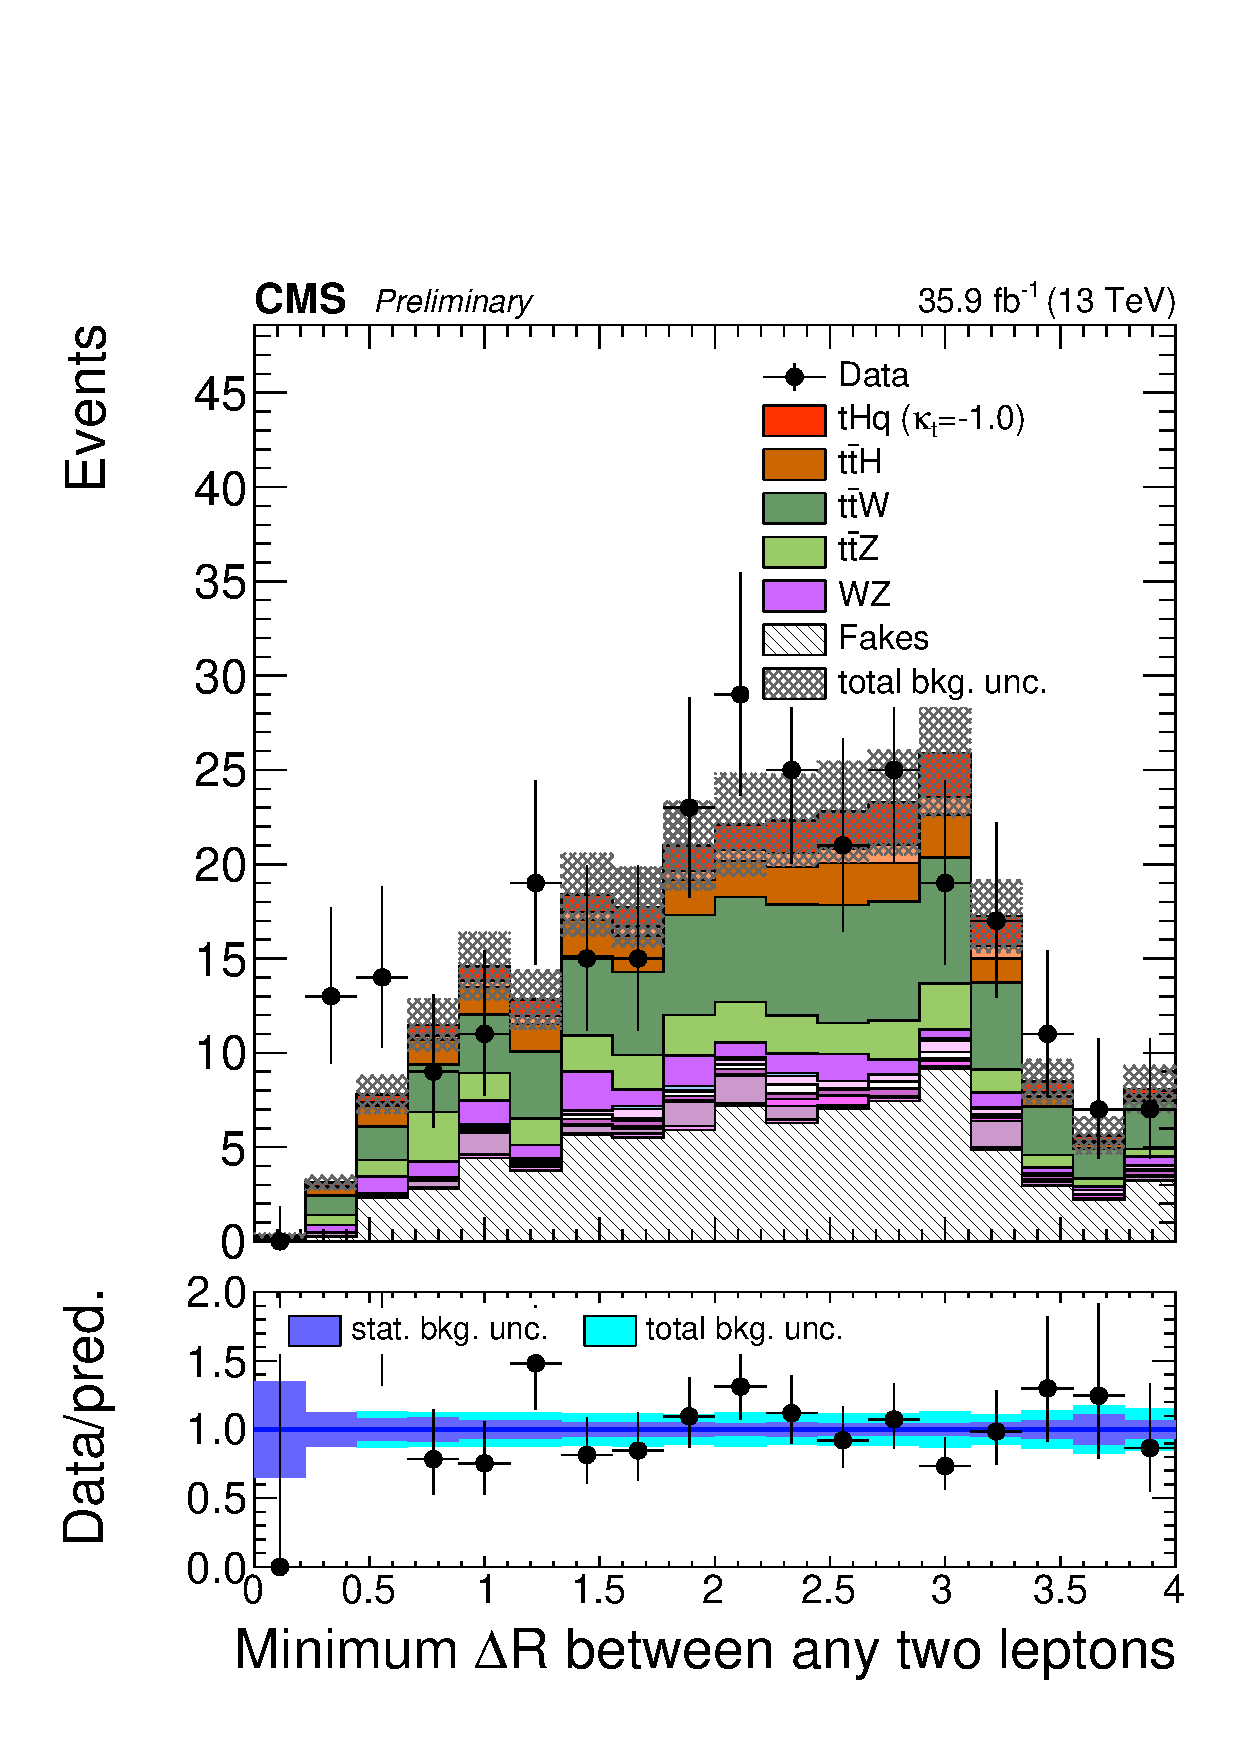
\includegraphics[width=0.22\textwidth]{figures/signalregion_2lss/mumu/minDRll.pdf} 
  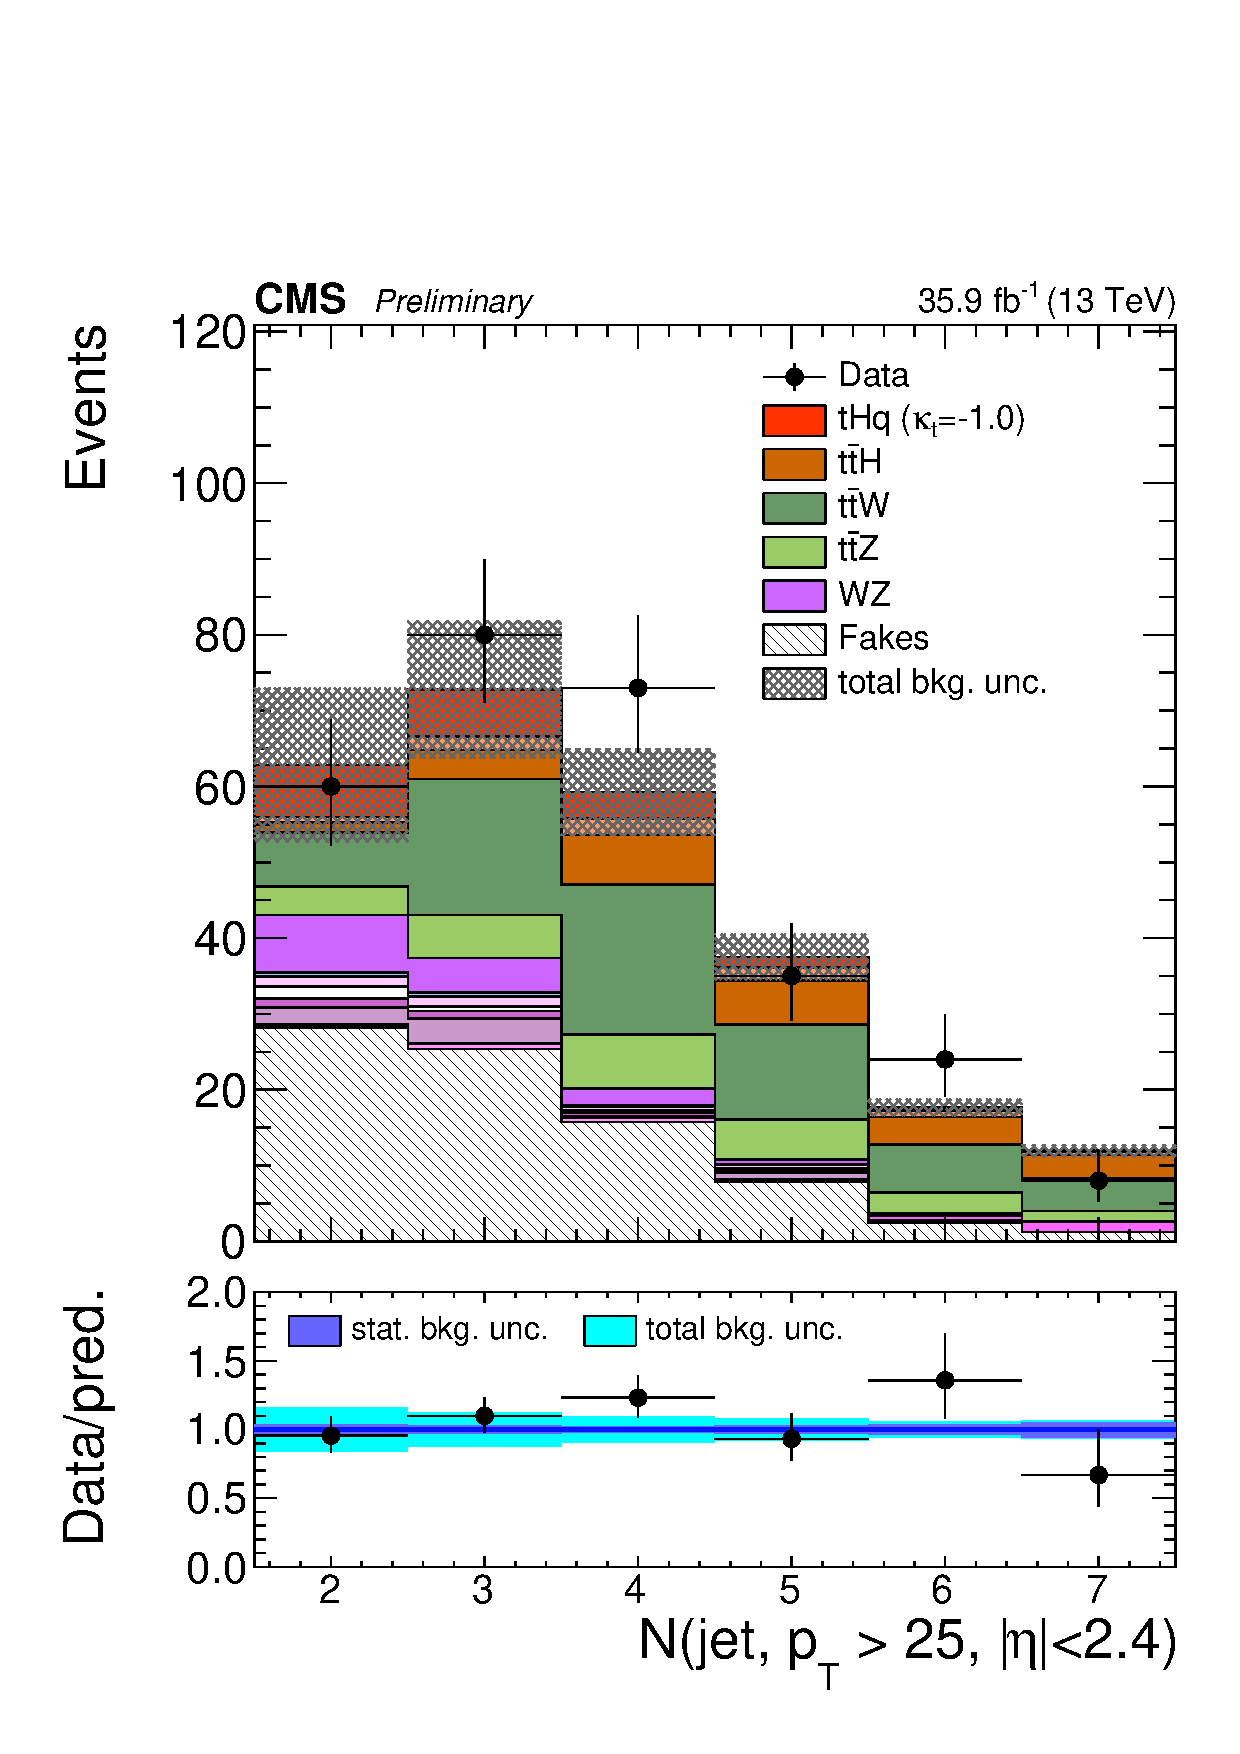
\includegraphics[width=0.22\textwidth]{figures/signalregion_2lss/mumu/nJet25.pdf} \\
  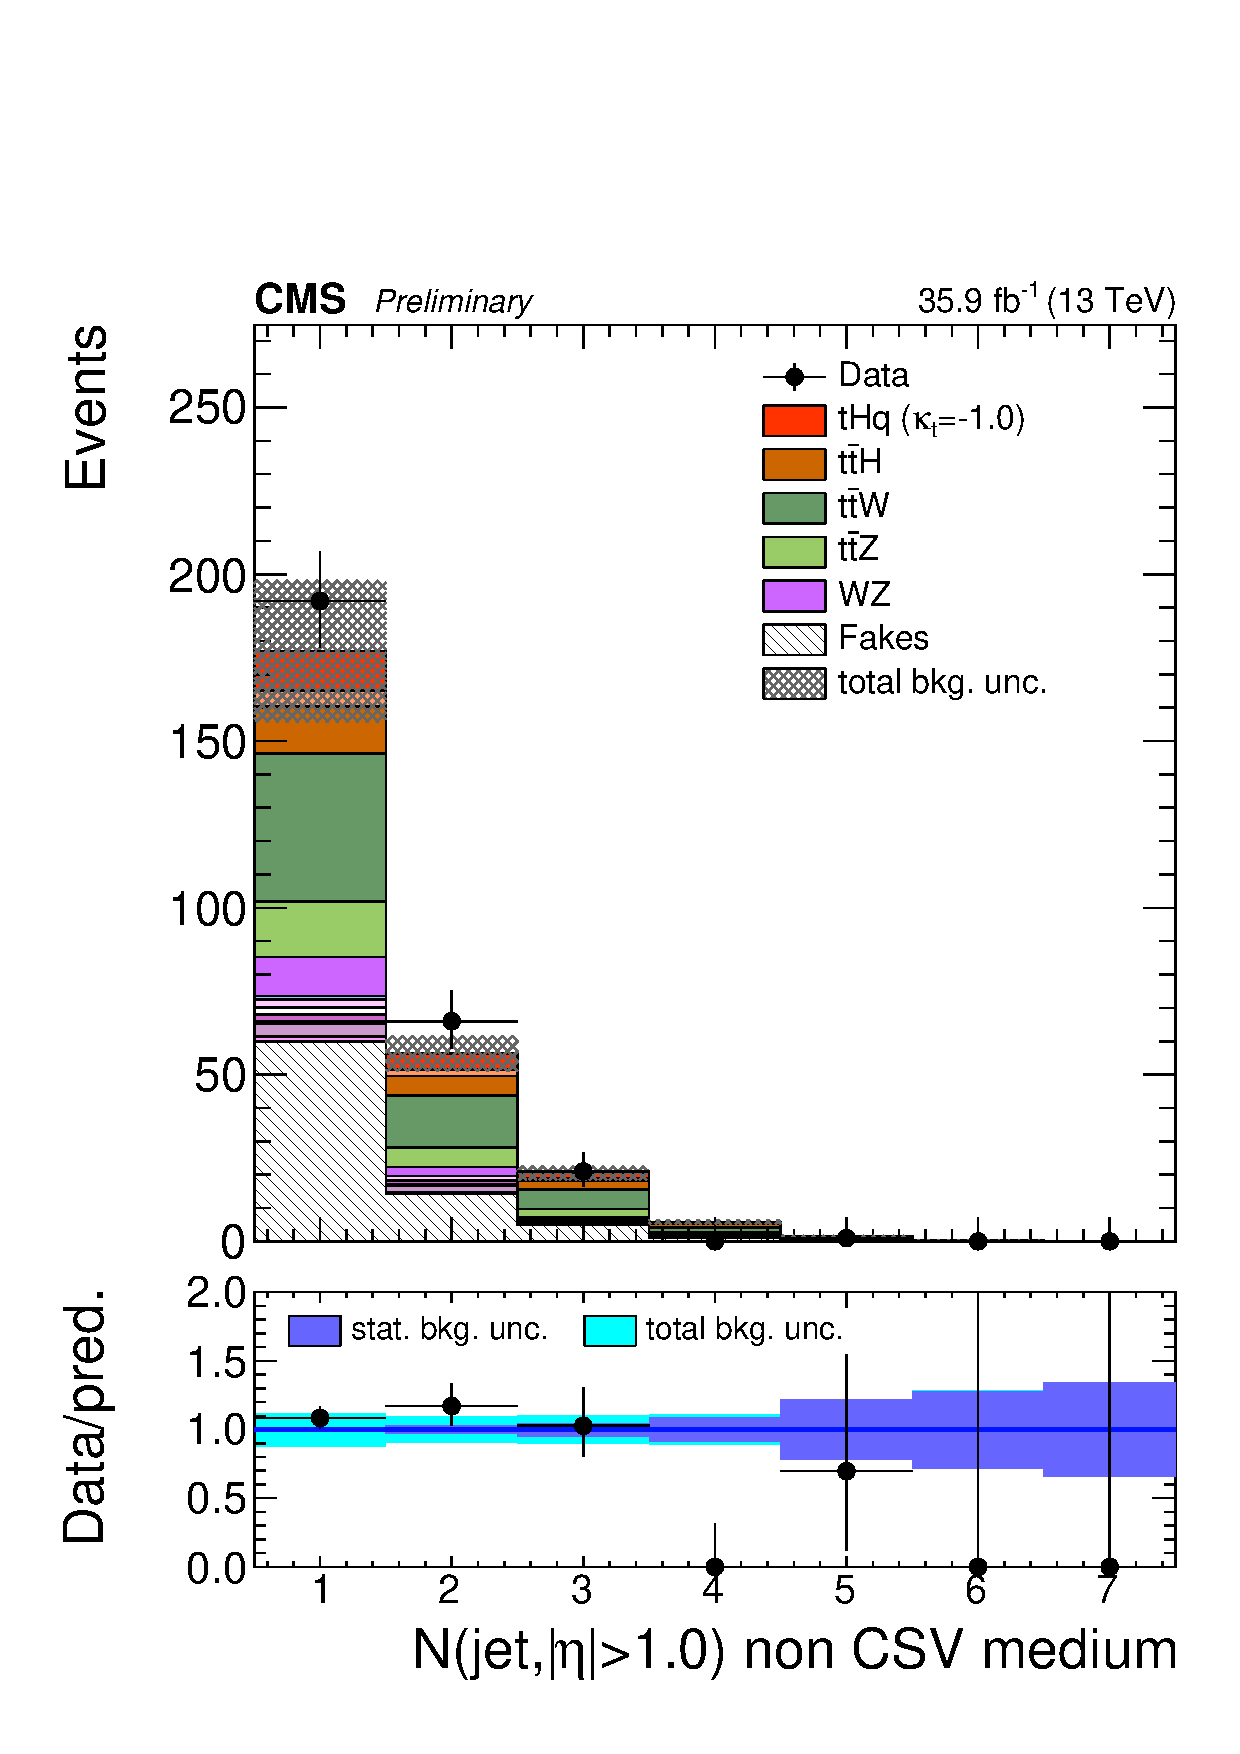
\includegraphics[width=0.22\textwidth]{figures/signalregion_2lss/mumu/nJetEta1_40.pdf}
  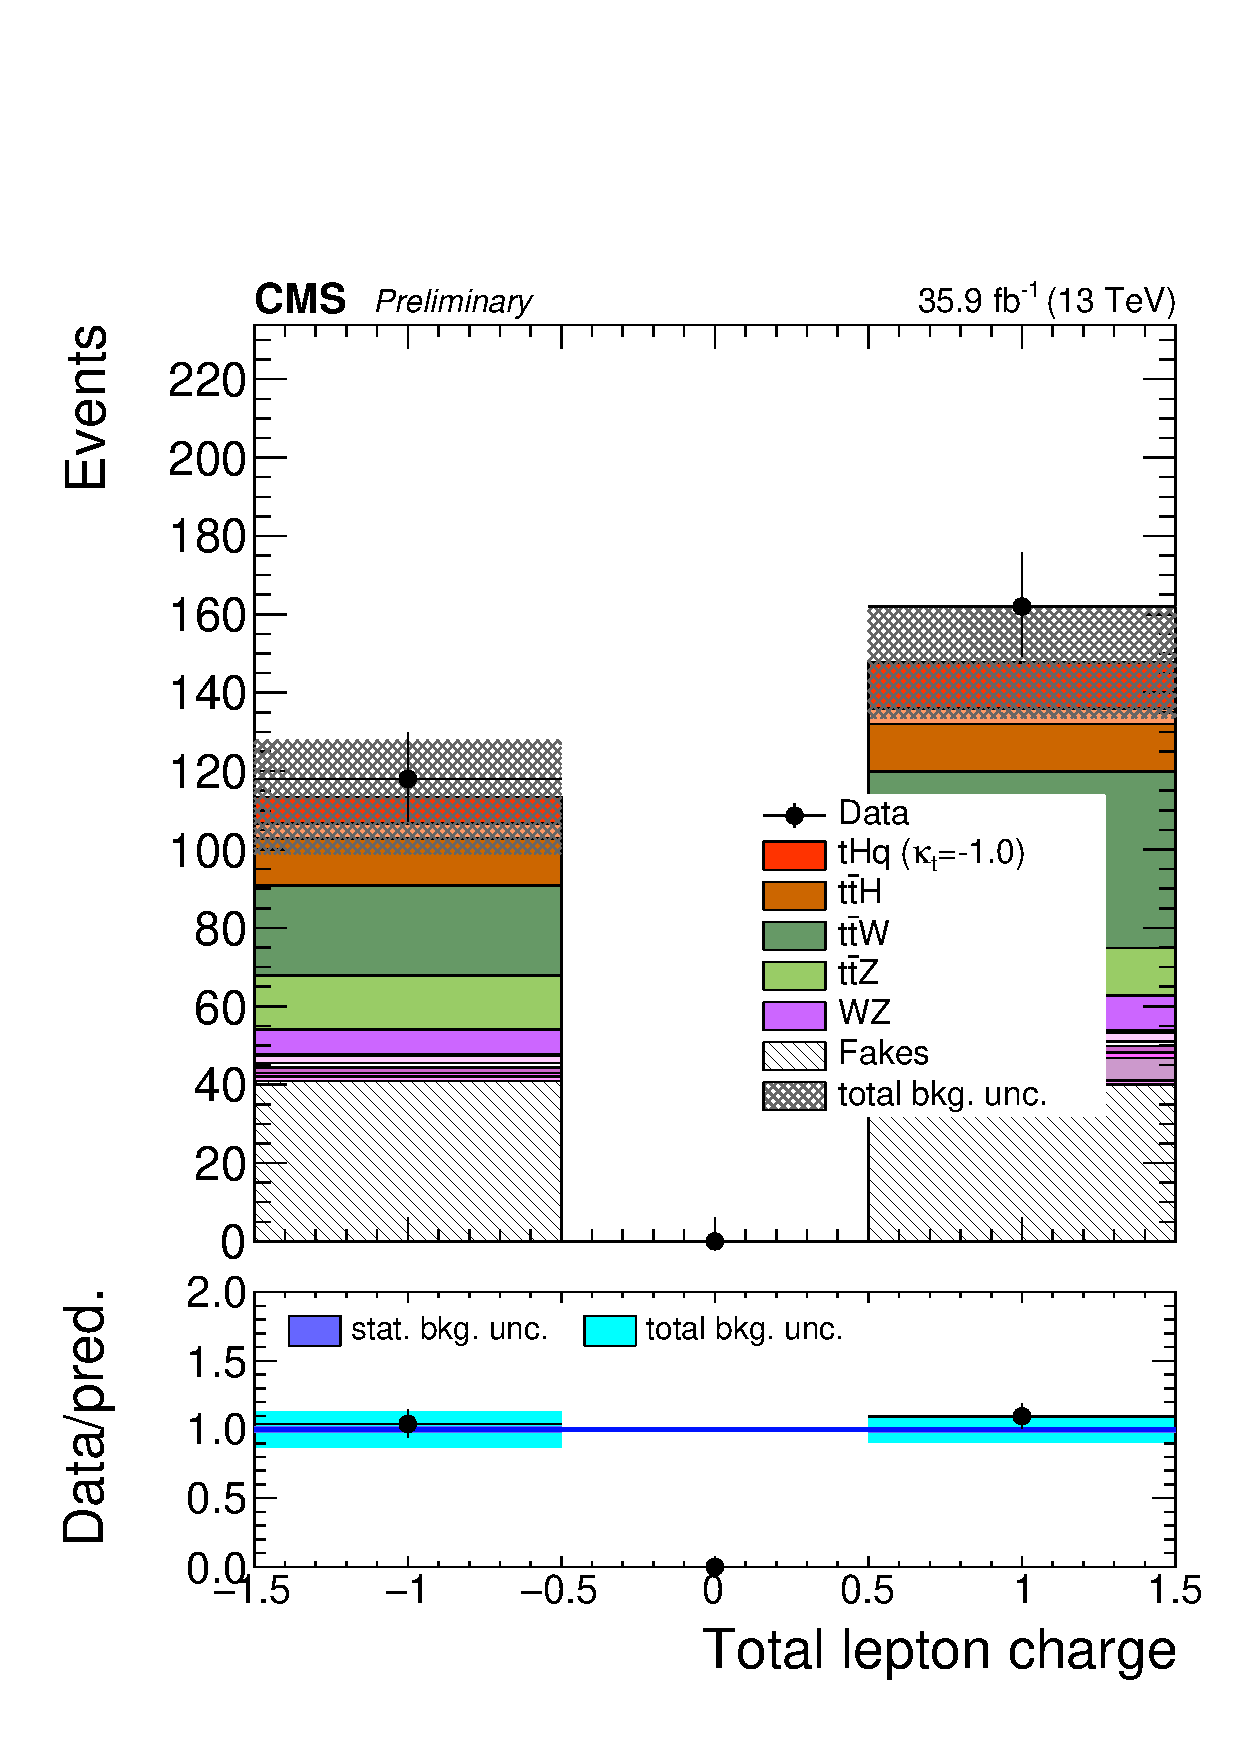
\includegraphics[width=0.22\textwidth]{figures/signalregion_2lss/mumu/totCharge.pdf}
\caption{Distributions of input variables to the BDT for signal discrimination, in \mumu\ channel, normalized to their cross section and to 35.9\fbinv.}
\label{fig:input_vars_2lss_xsec_mumu}
\end{figure}

\begin{figure} [!h]
  \centering
  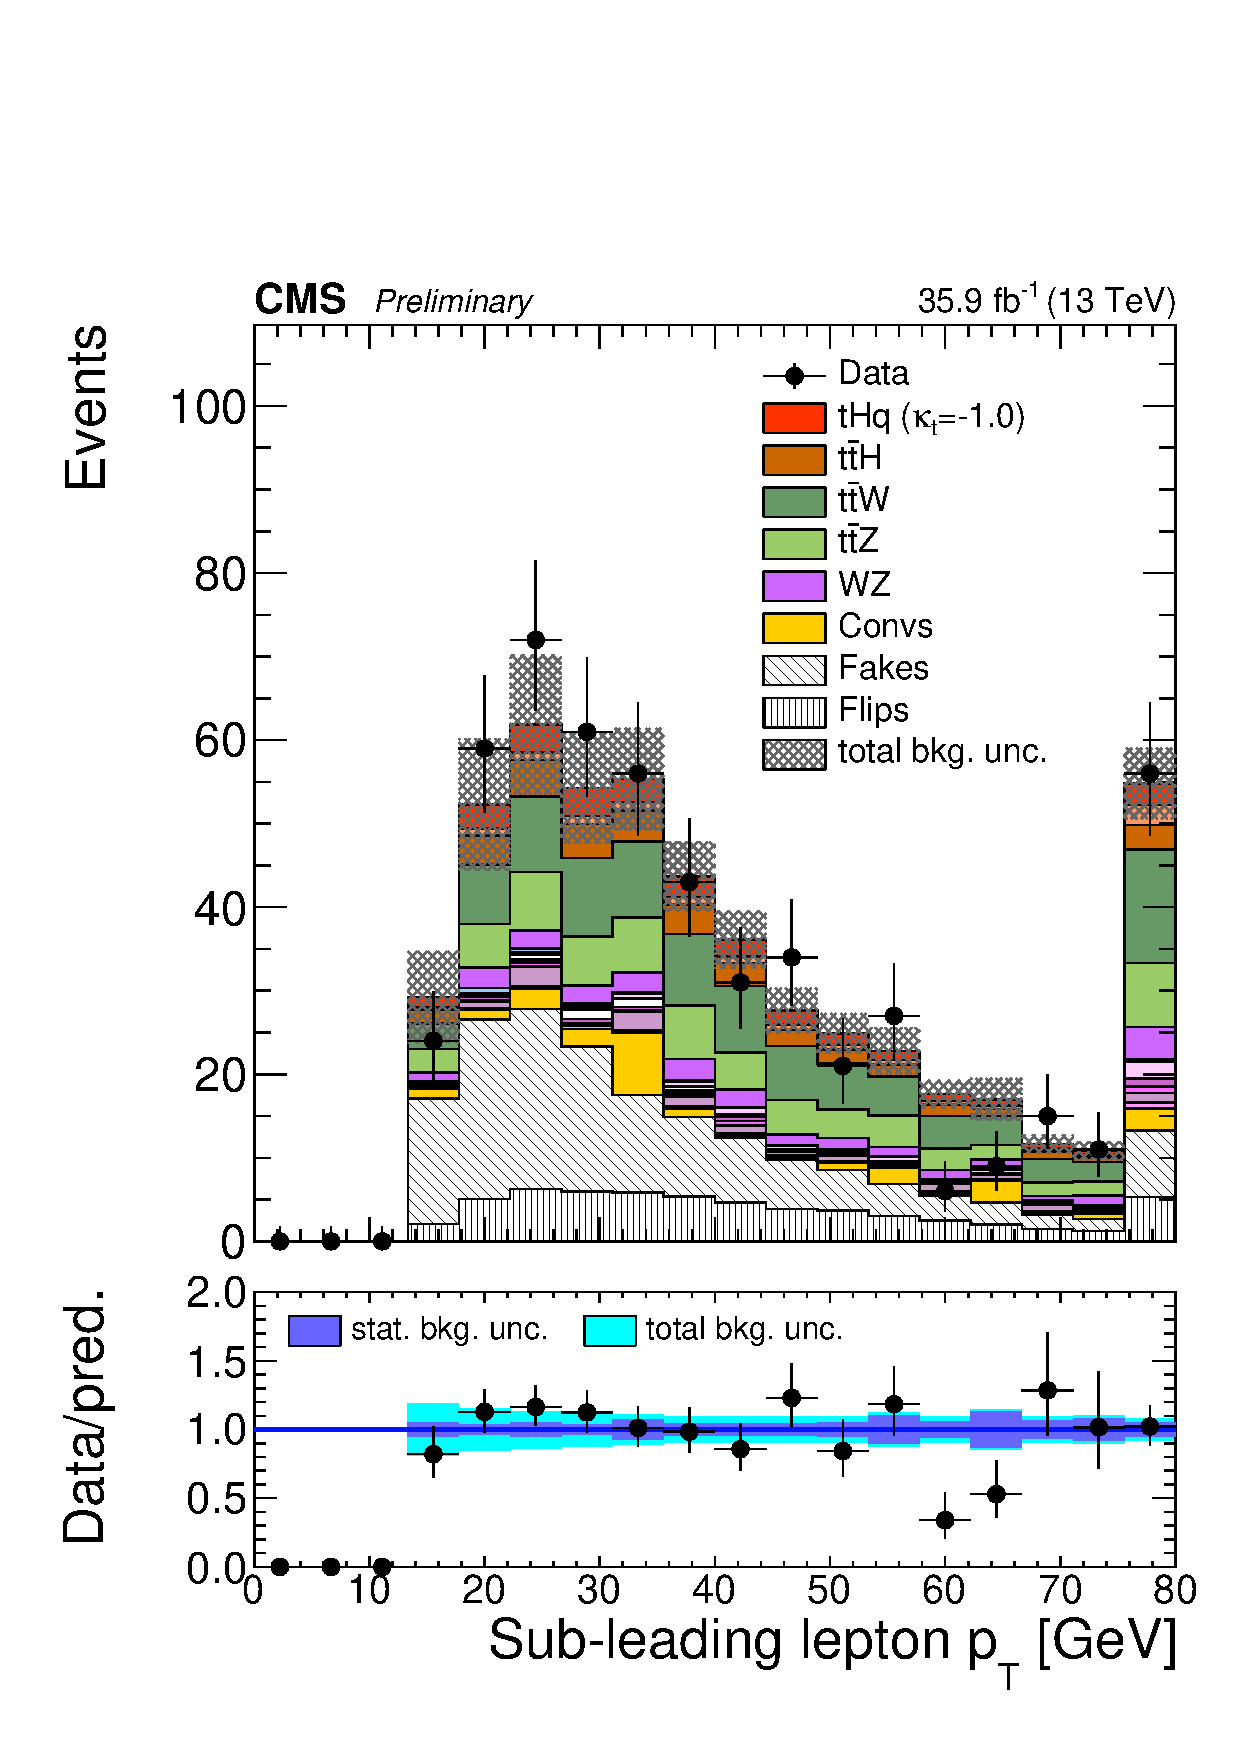
\includegraphics[width=0.22\textwidth]{figures/signalregion_2lss/emu/Lep2Pt.pdf}
  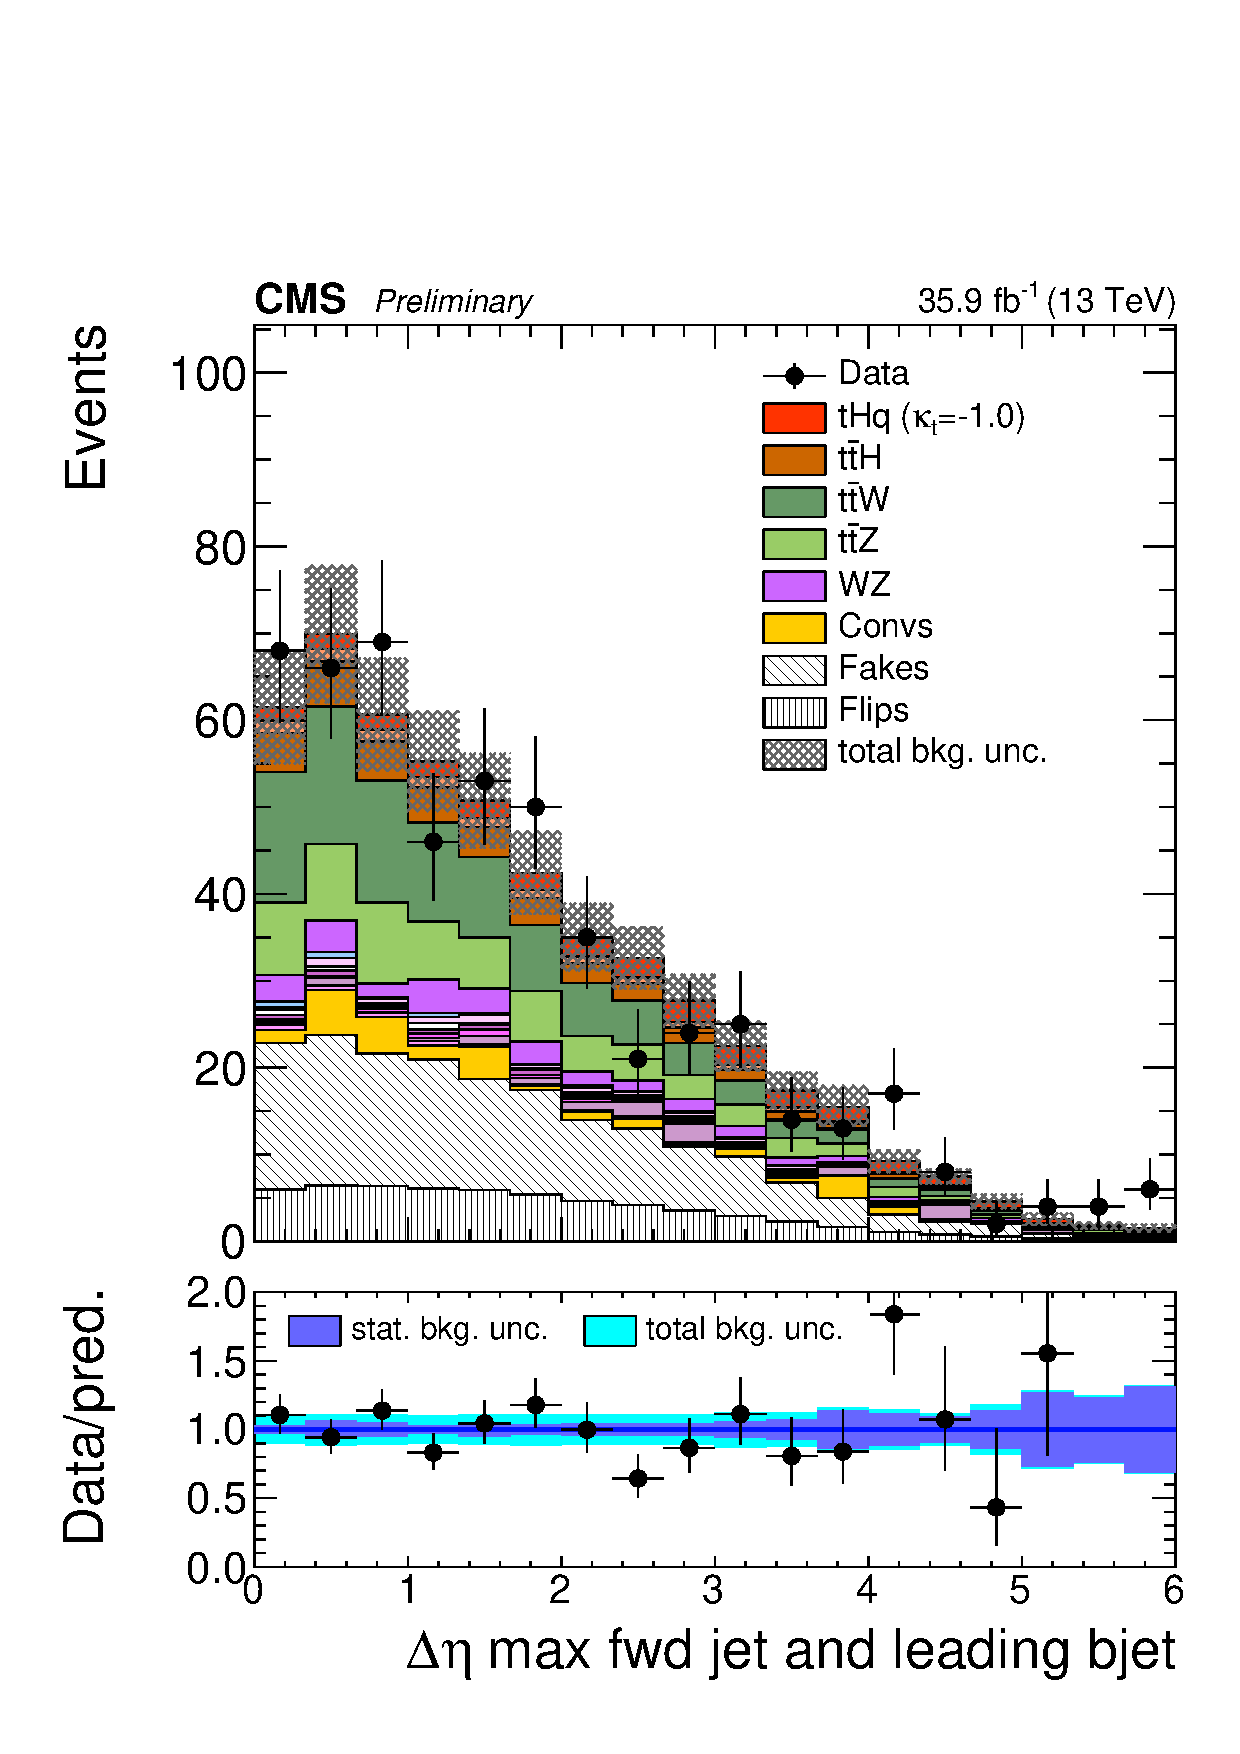
\includegraphics[width=0.22\textwidth]{figures/signalregion_2lss/emu/dEtaFwdJetBJet_40.pdf}
  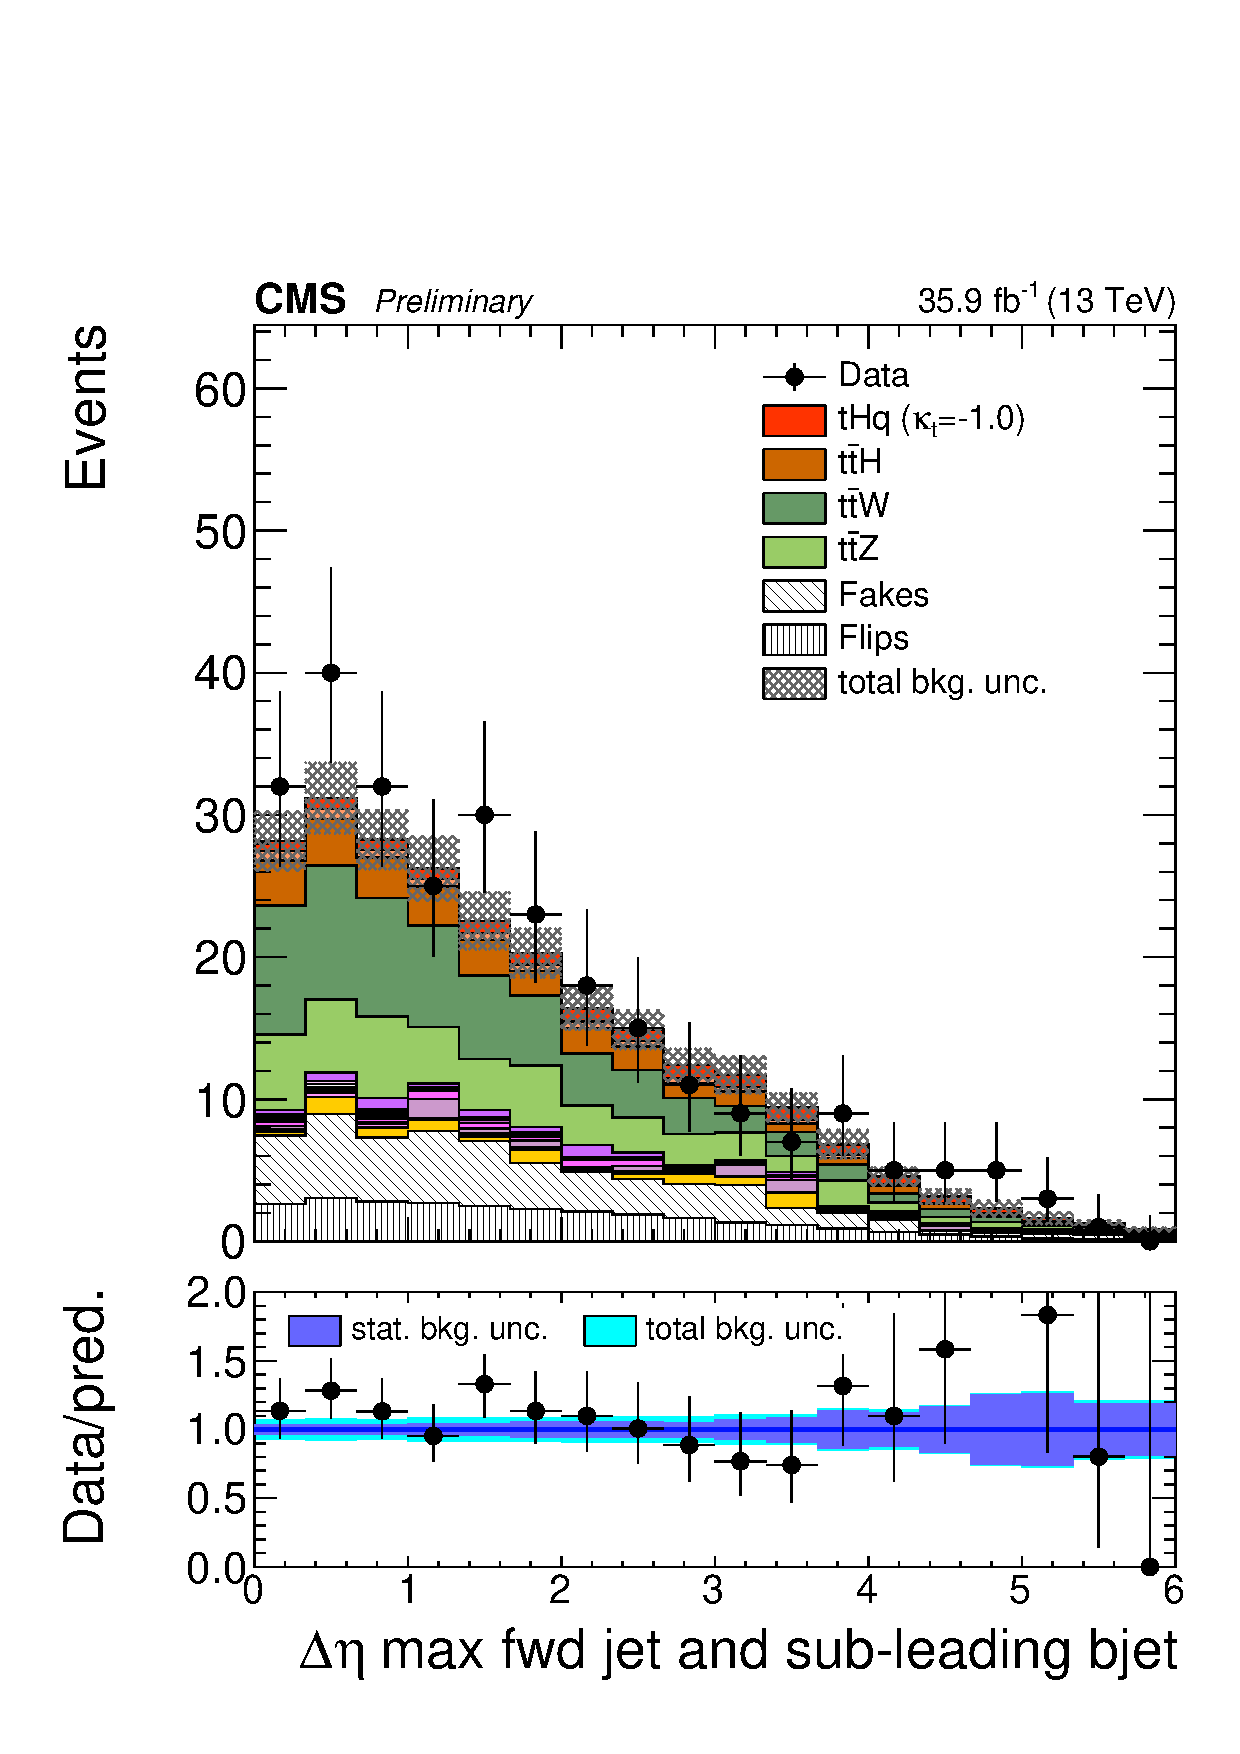
\includegraphics[width=0.22\textwidth]{figures/signalregion_2lss/emu/dEtaFwdJet2BJet_40.pdf}
  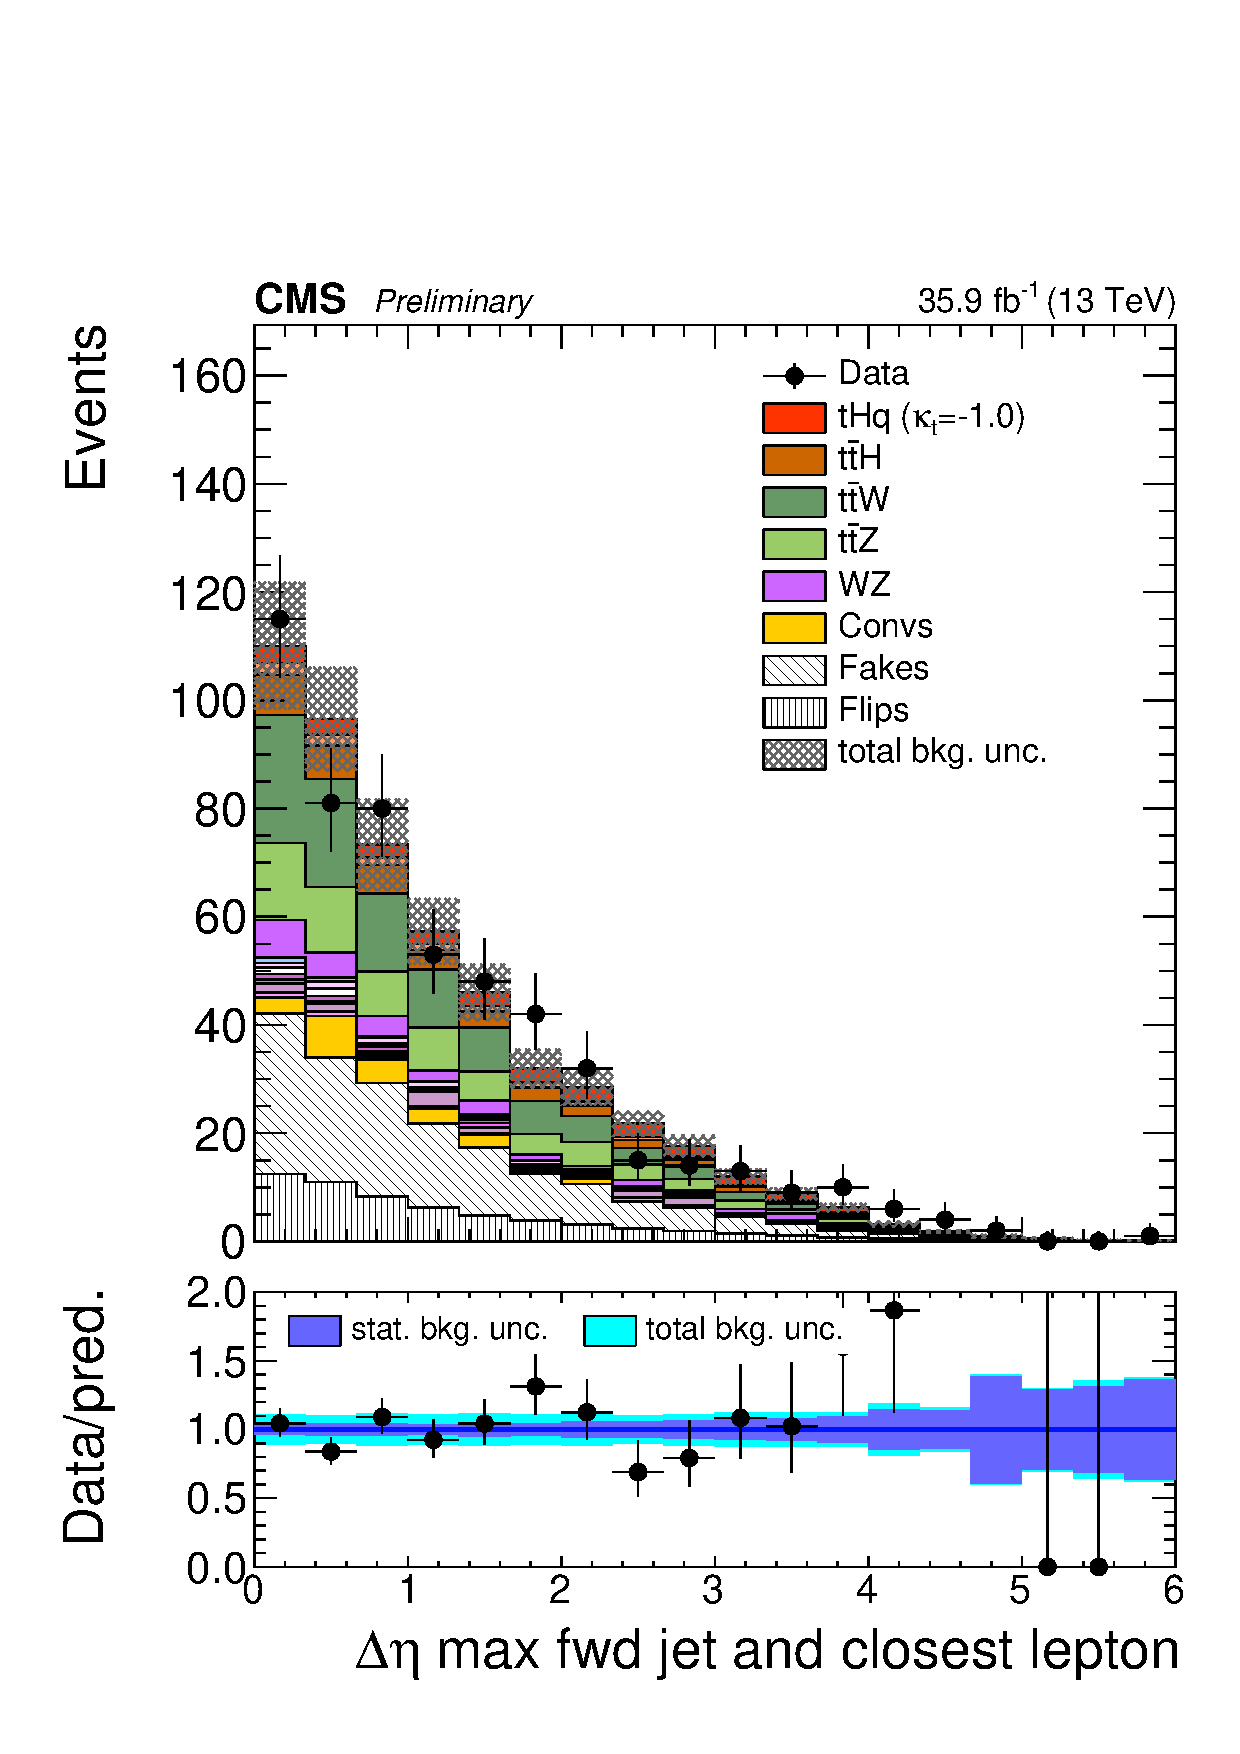
\includegraphics[width=0.22\textwidth]{figures/signalregion_2lss/emu/dEtaFwdJetClosestLep_40.pdf} \\
  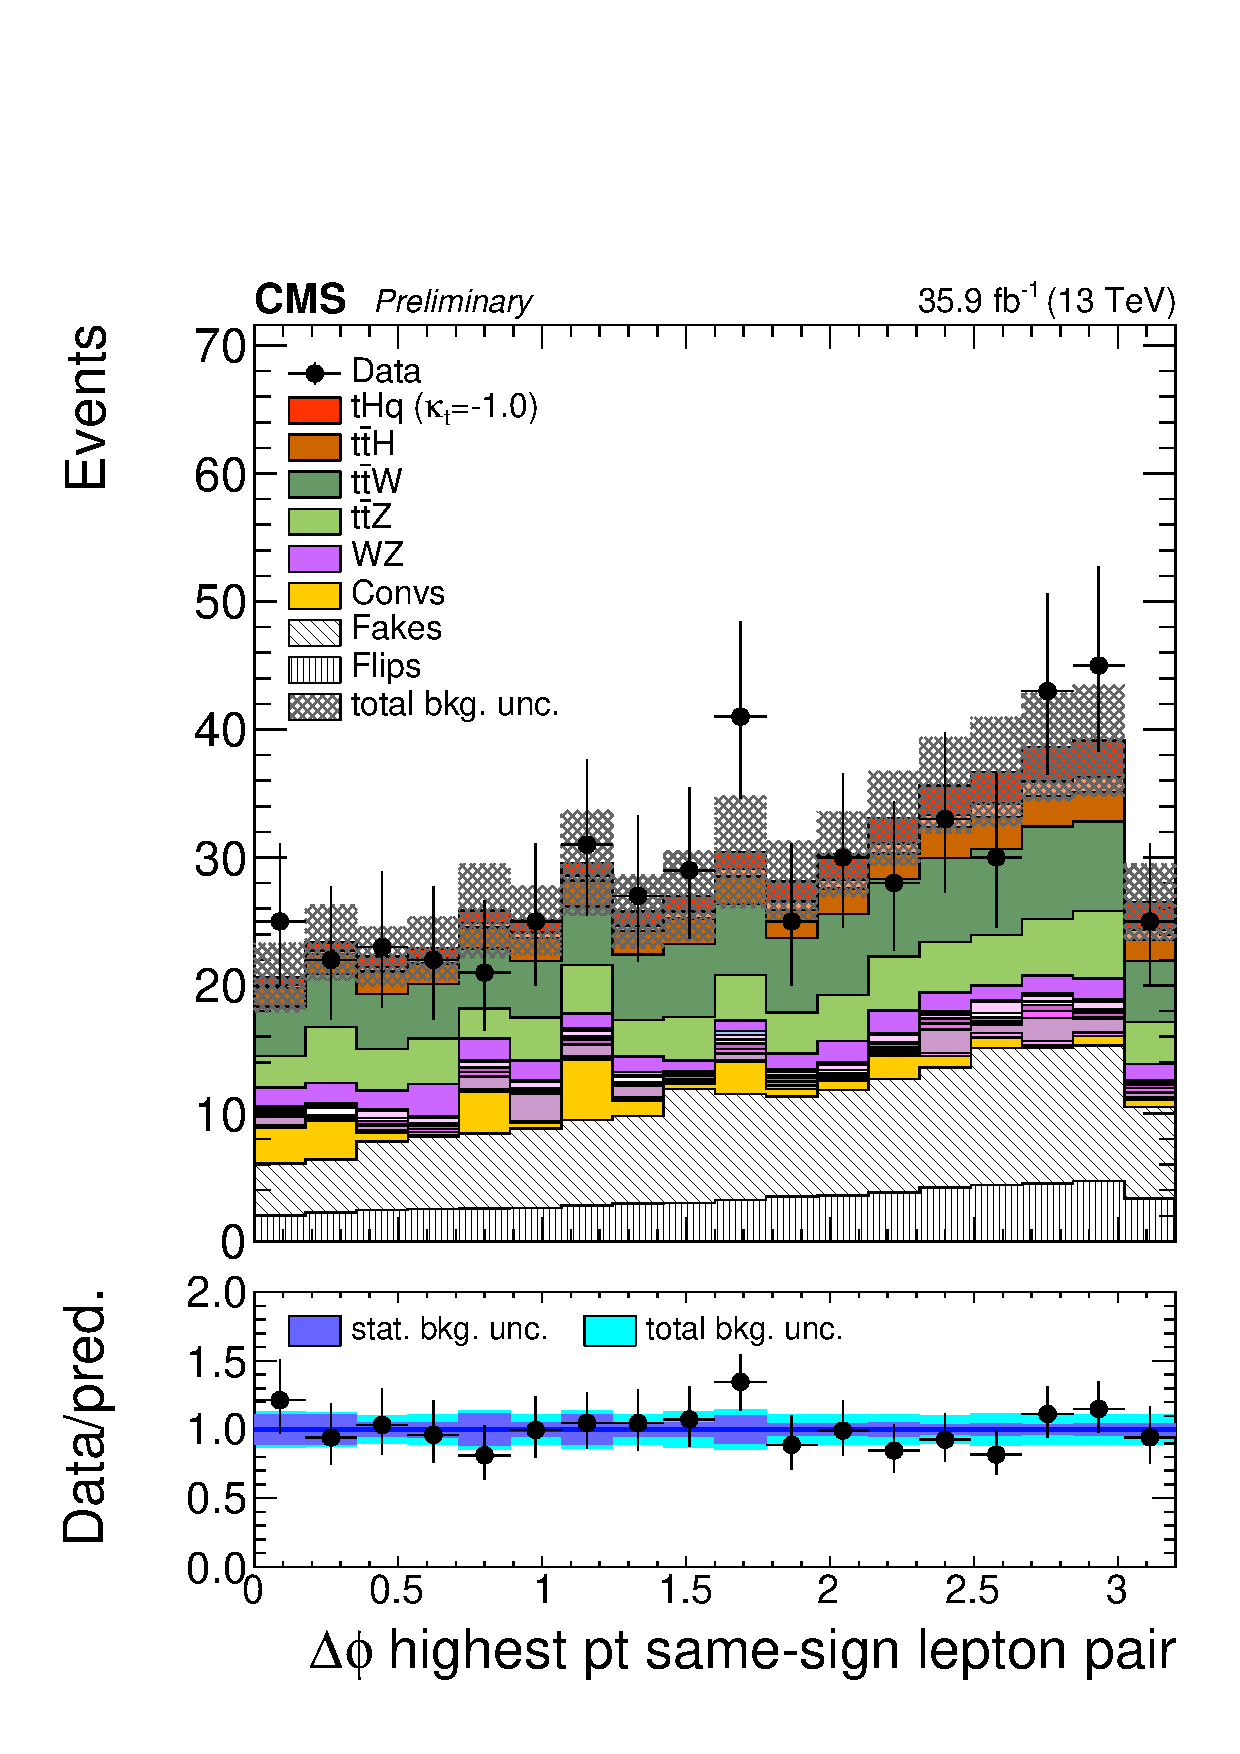
\includegraphics[width=0.22\textwidth]{figures/signalregion_2lss/emu/dPhiHighestPtSSPair.pdf}
  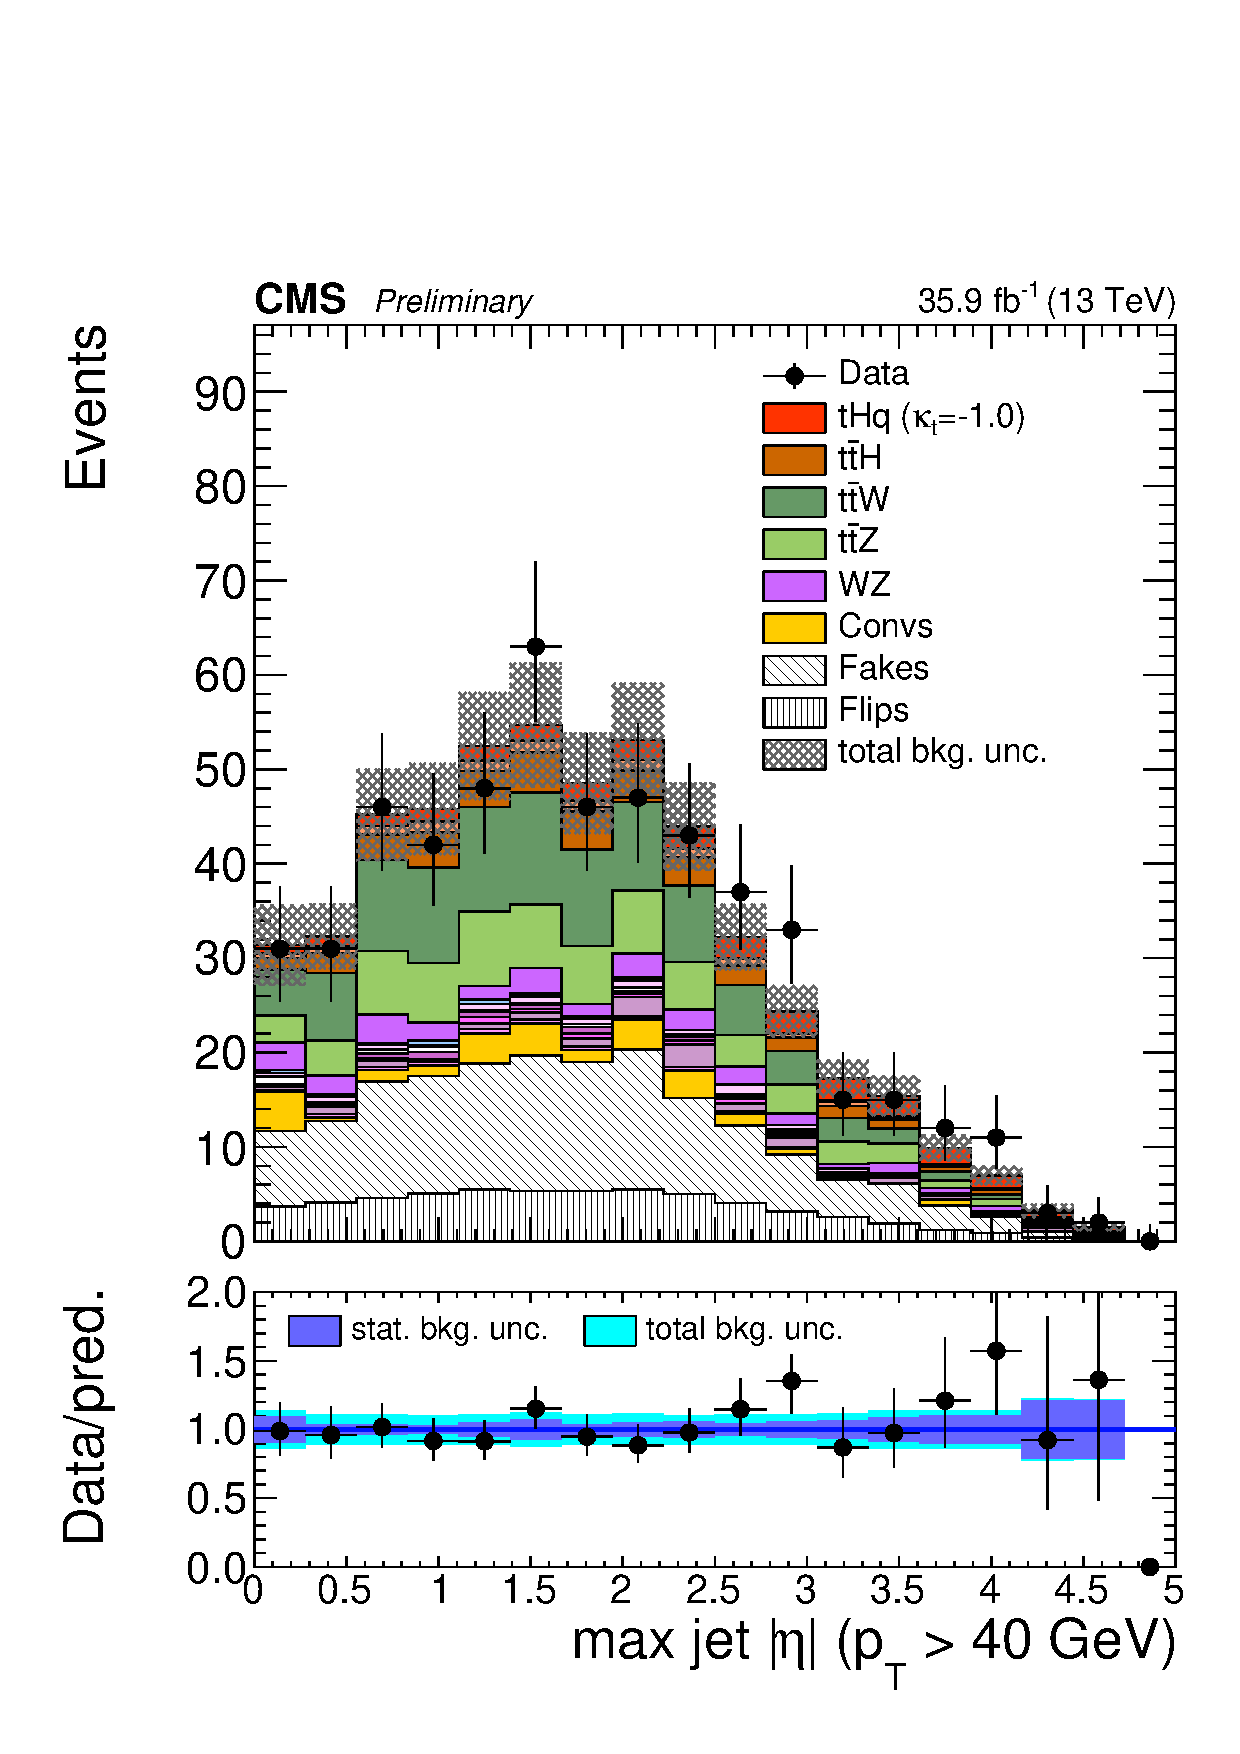
\includegraphics[width=0.22\textwidth]{figures/signalregion_2lss/emu/maxEtaJet25_40.pdf}
  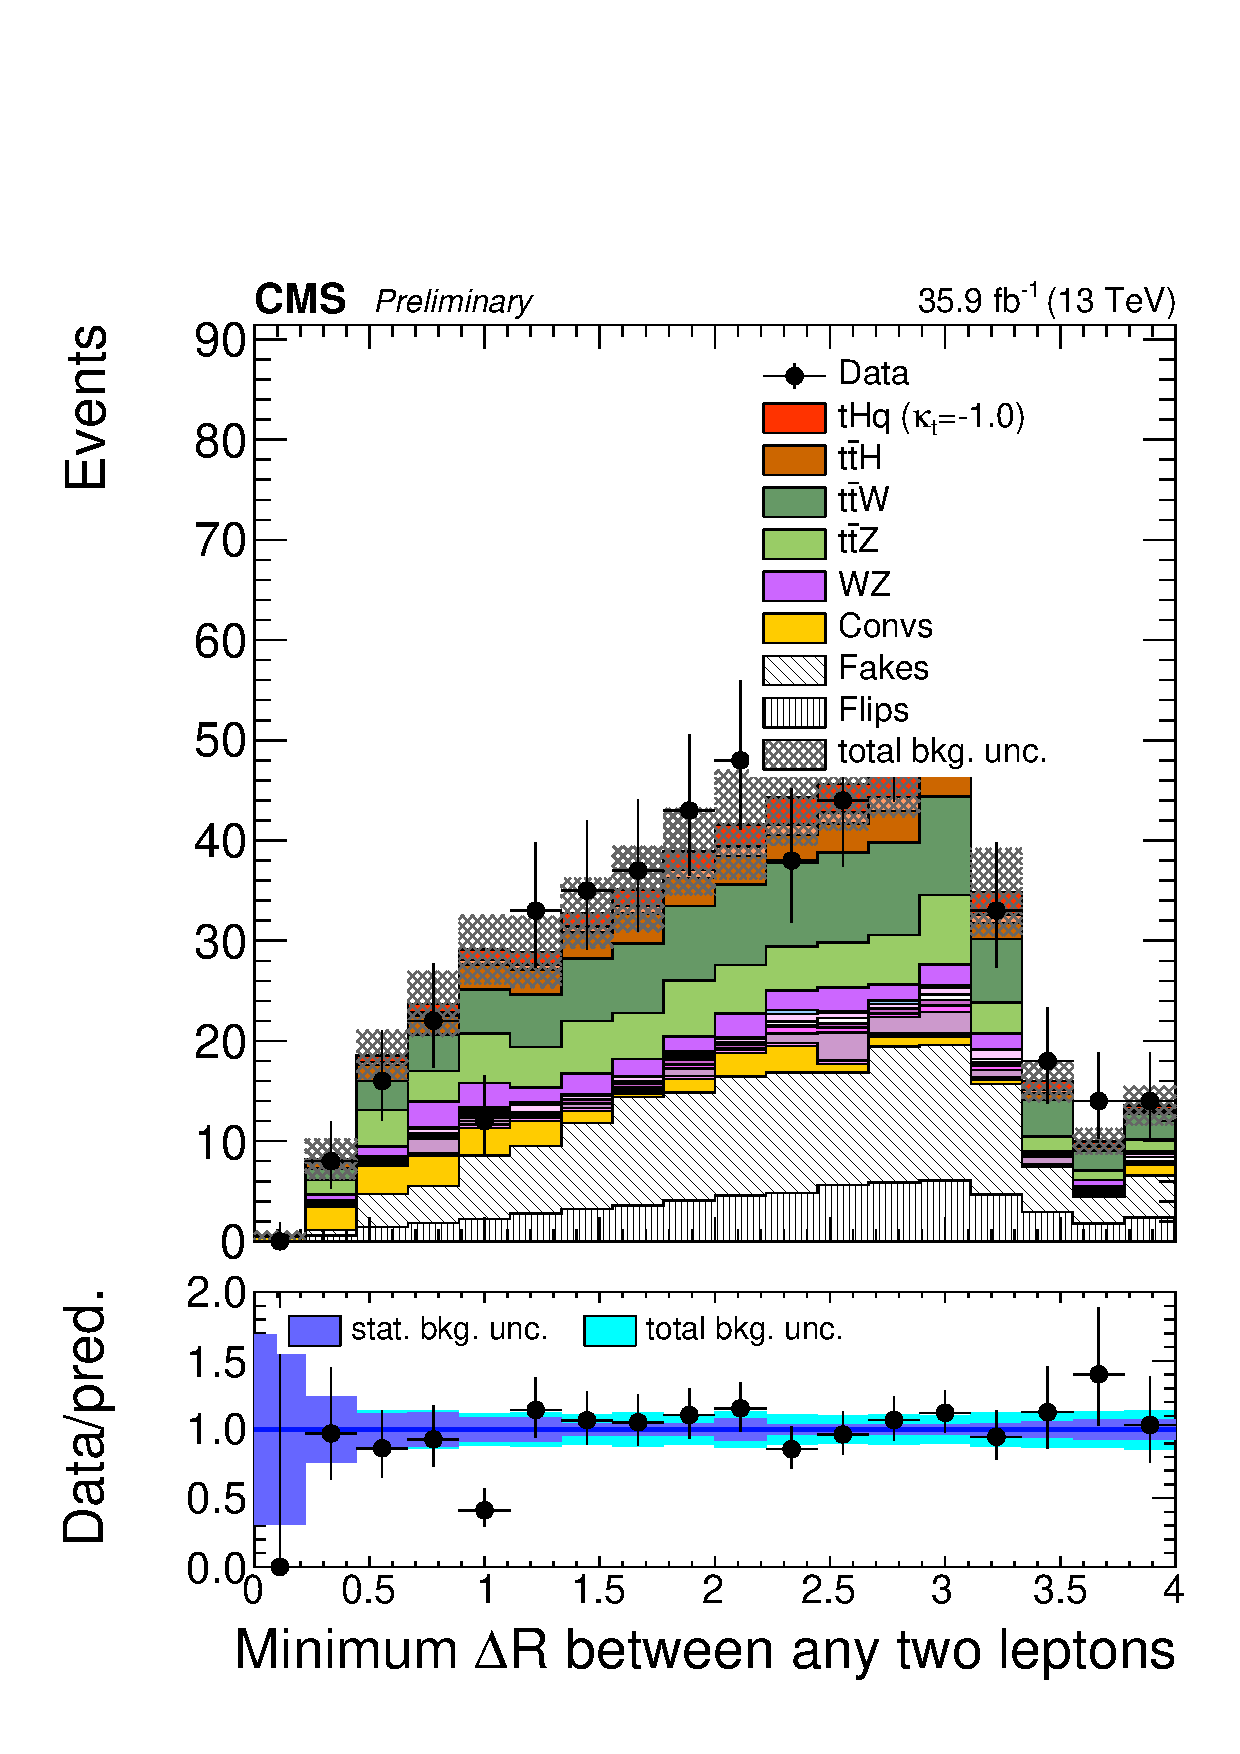
\includegraphics[width=0.22\textwidth]{figures/signalregion_2lss/emu/minDRll.pdf} 
  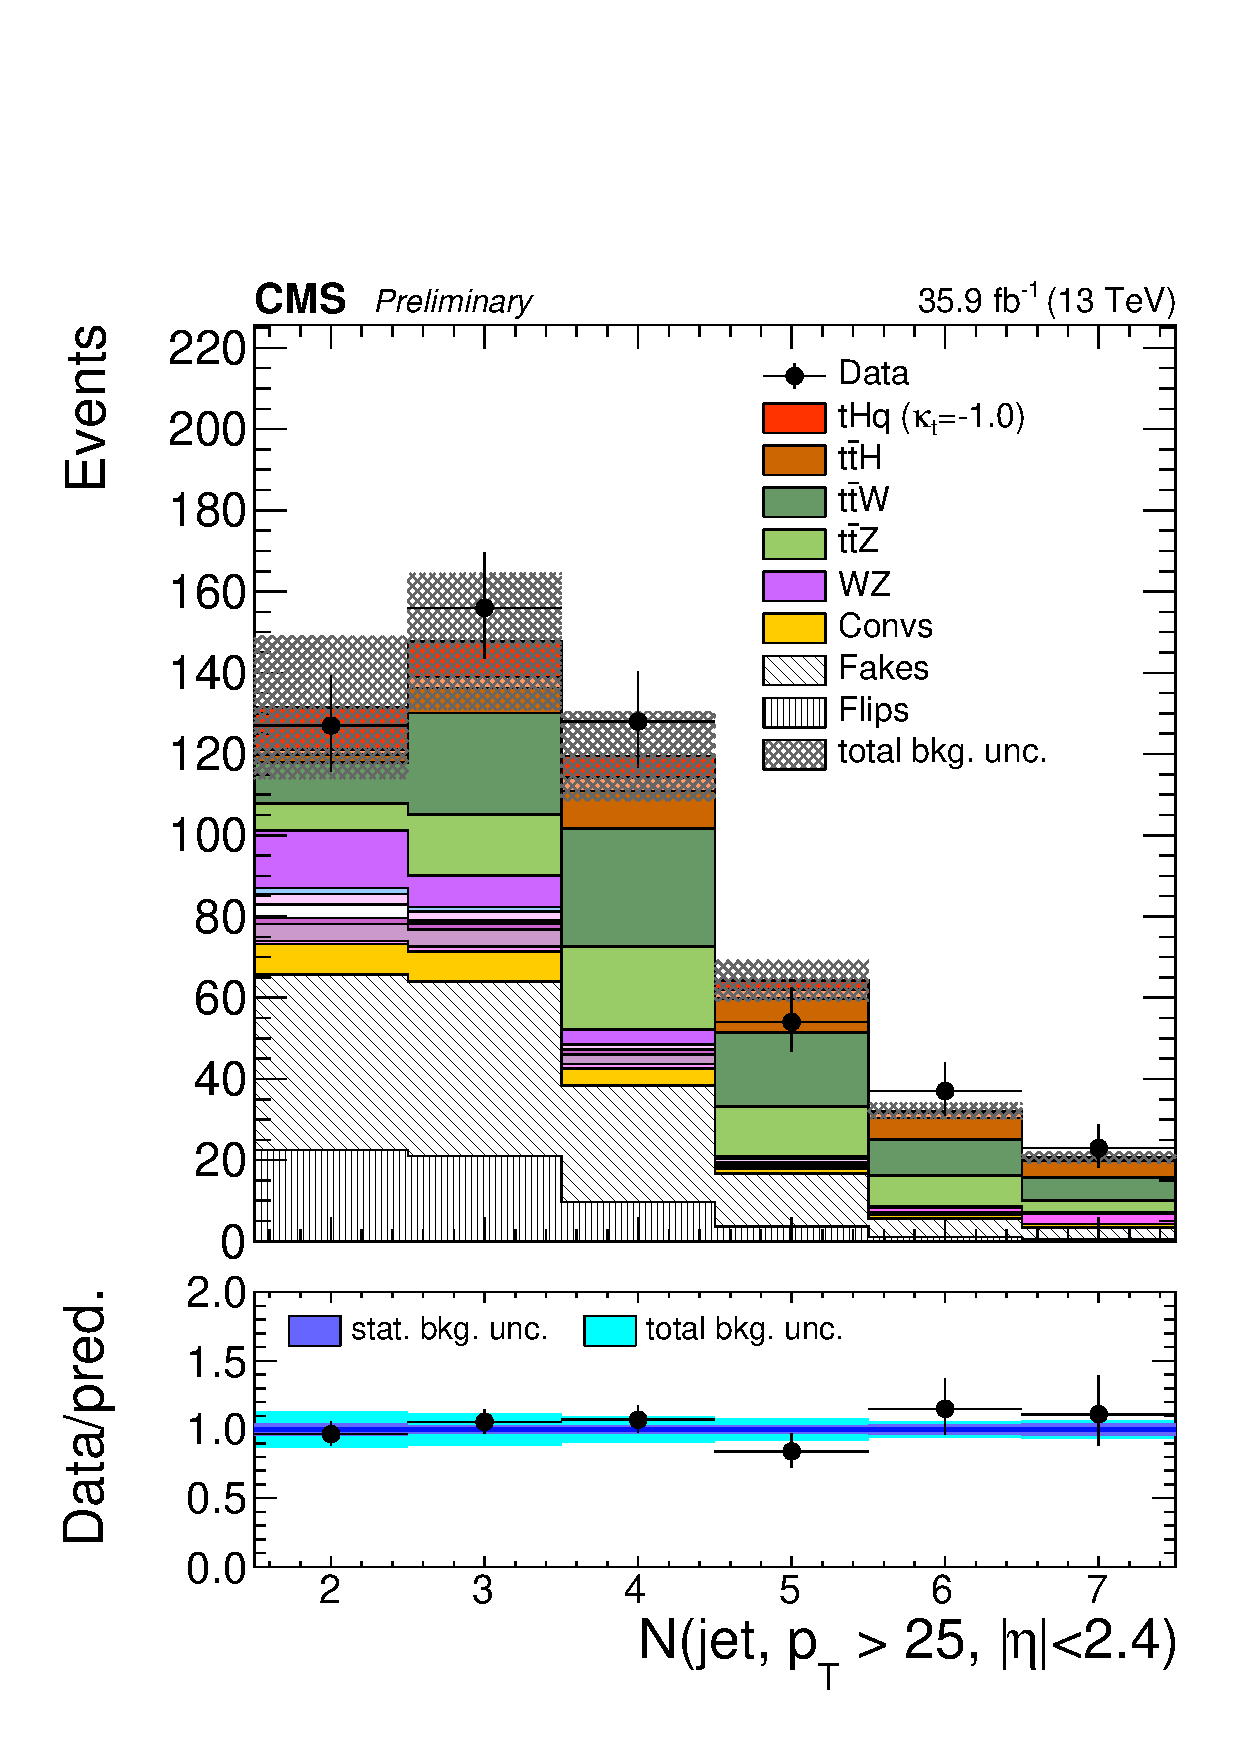
\includegraphics[width=0.22\textwidth]{figures/signalregion_2lss/emu/nJet25.pdf} \\
  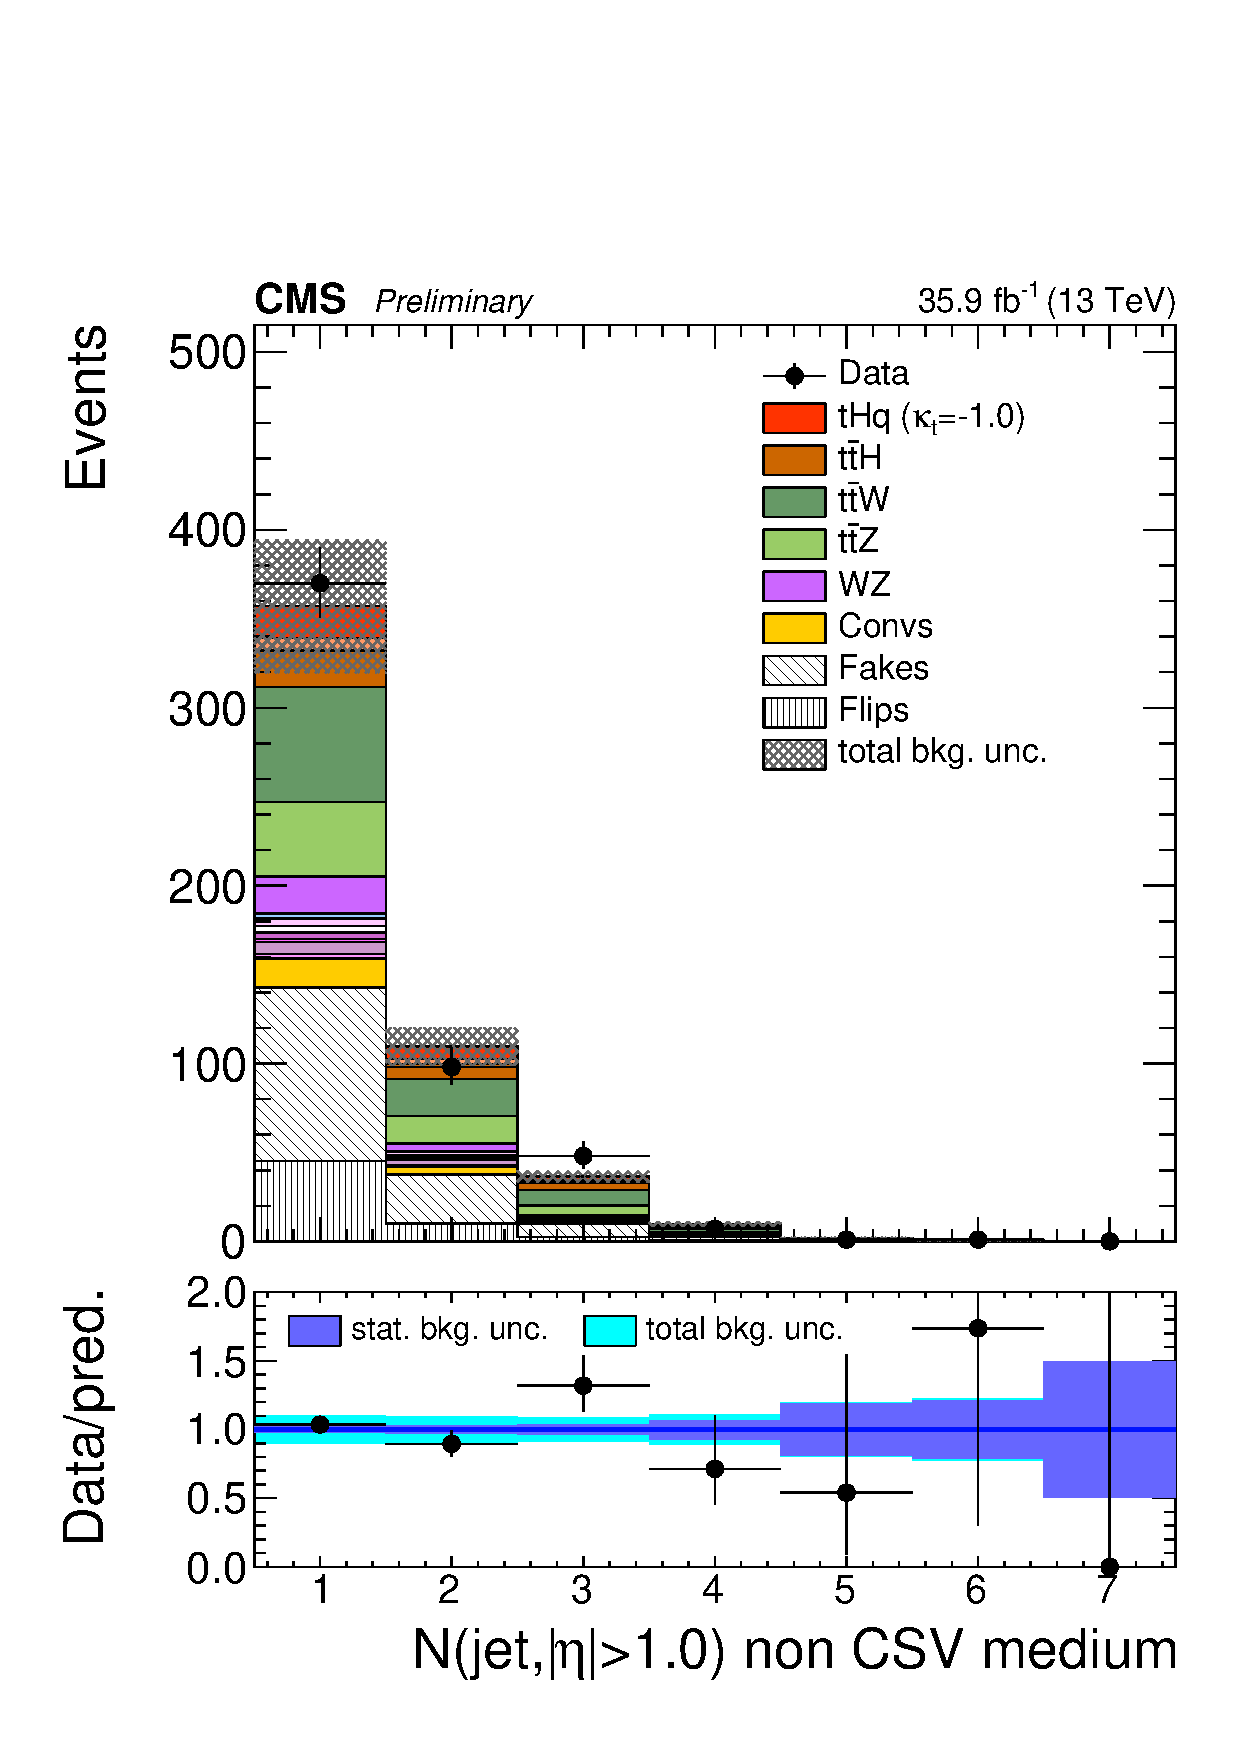
\includegraphics[width=0.22\textwidth]{figures/signalregion_2lss/emu/nJetEta1_40.pdf}
  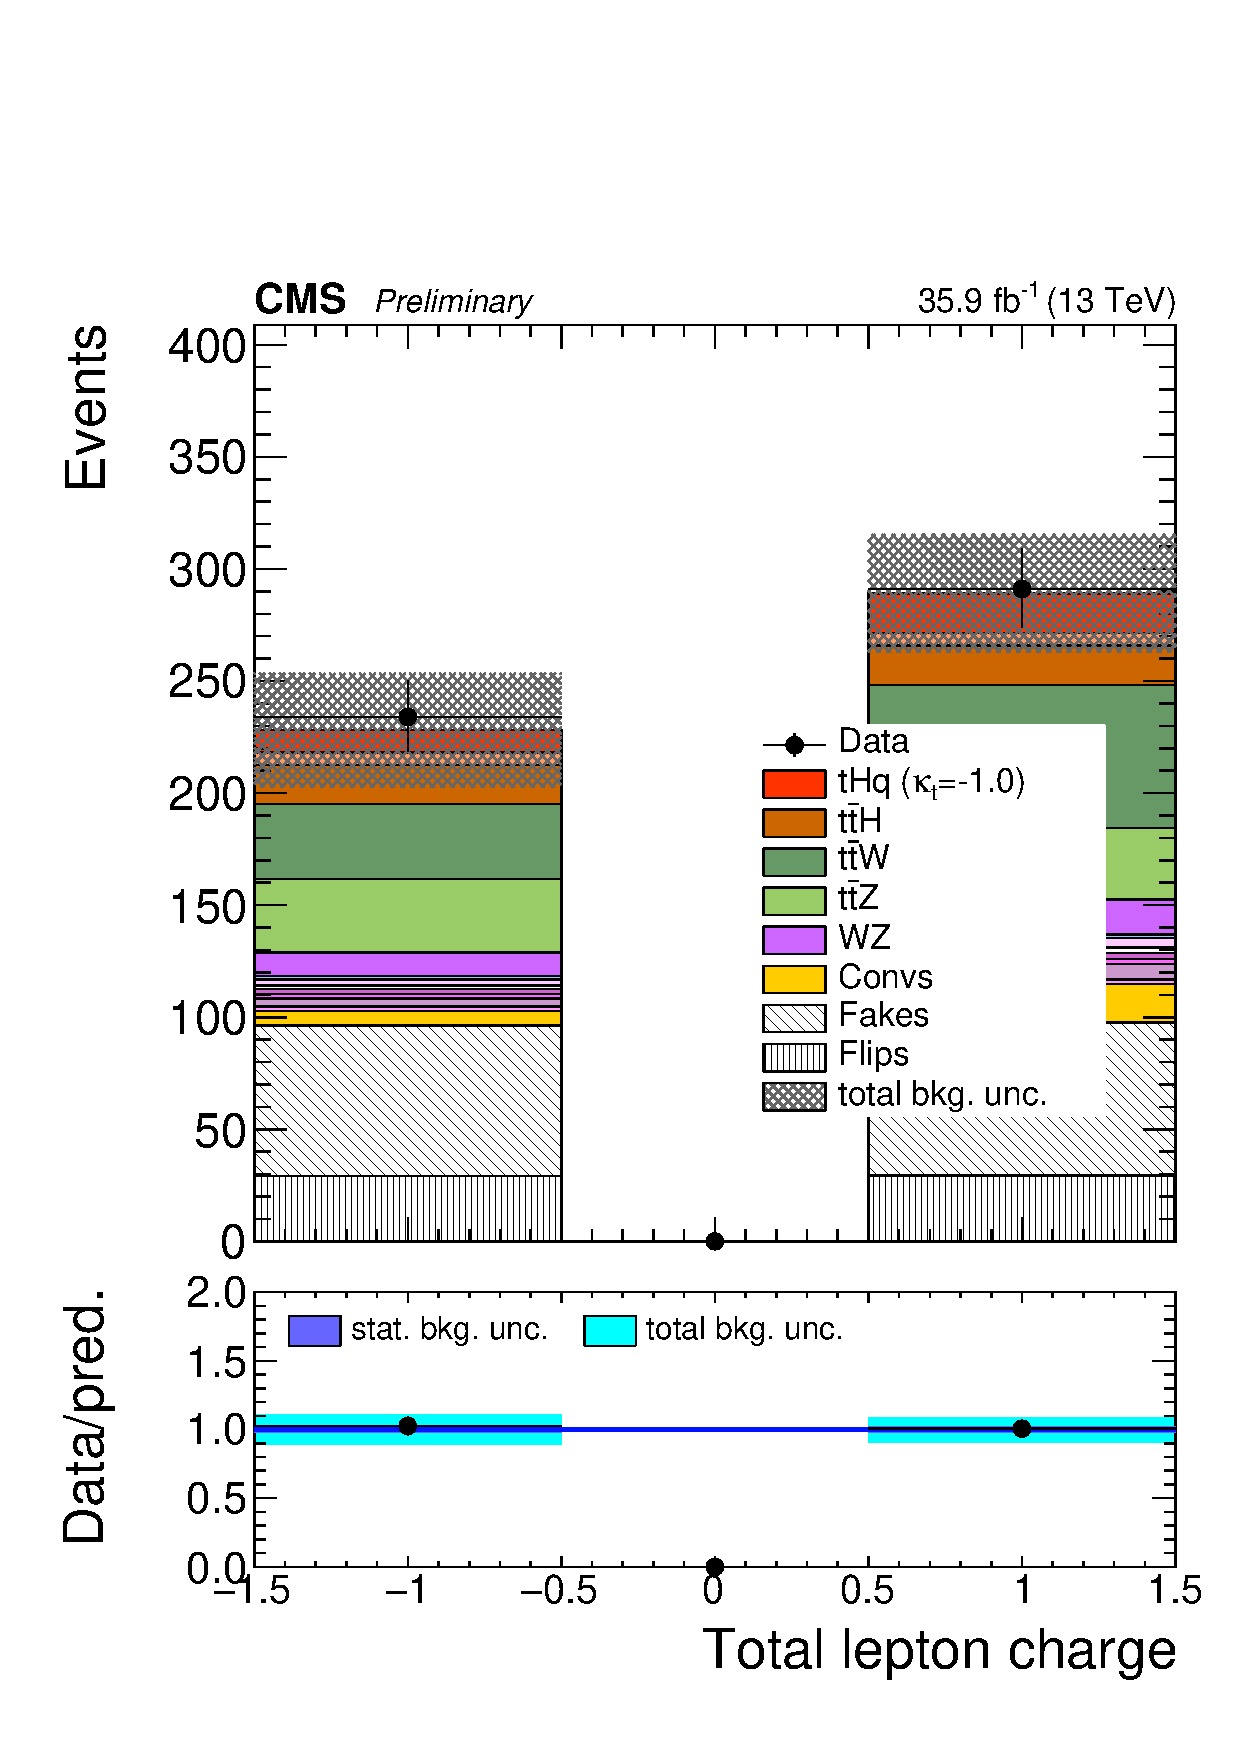
\includegraphics[width=0.22\textwidth]{figures/signalregion_2lss/emu/totCharge.pdf}
\caption{Distributions of input variables to the BDT for signal discrimination, in $e^{\pm}\mu^{\pm}$ channel, normalized to their cross section and to 35.9\fbinv.}
\label{fig:input_vars_2lss_xsec_emu}
\end{figure}

\begin{figure} [!h]
  \centering
  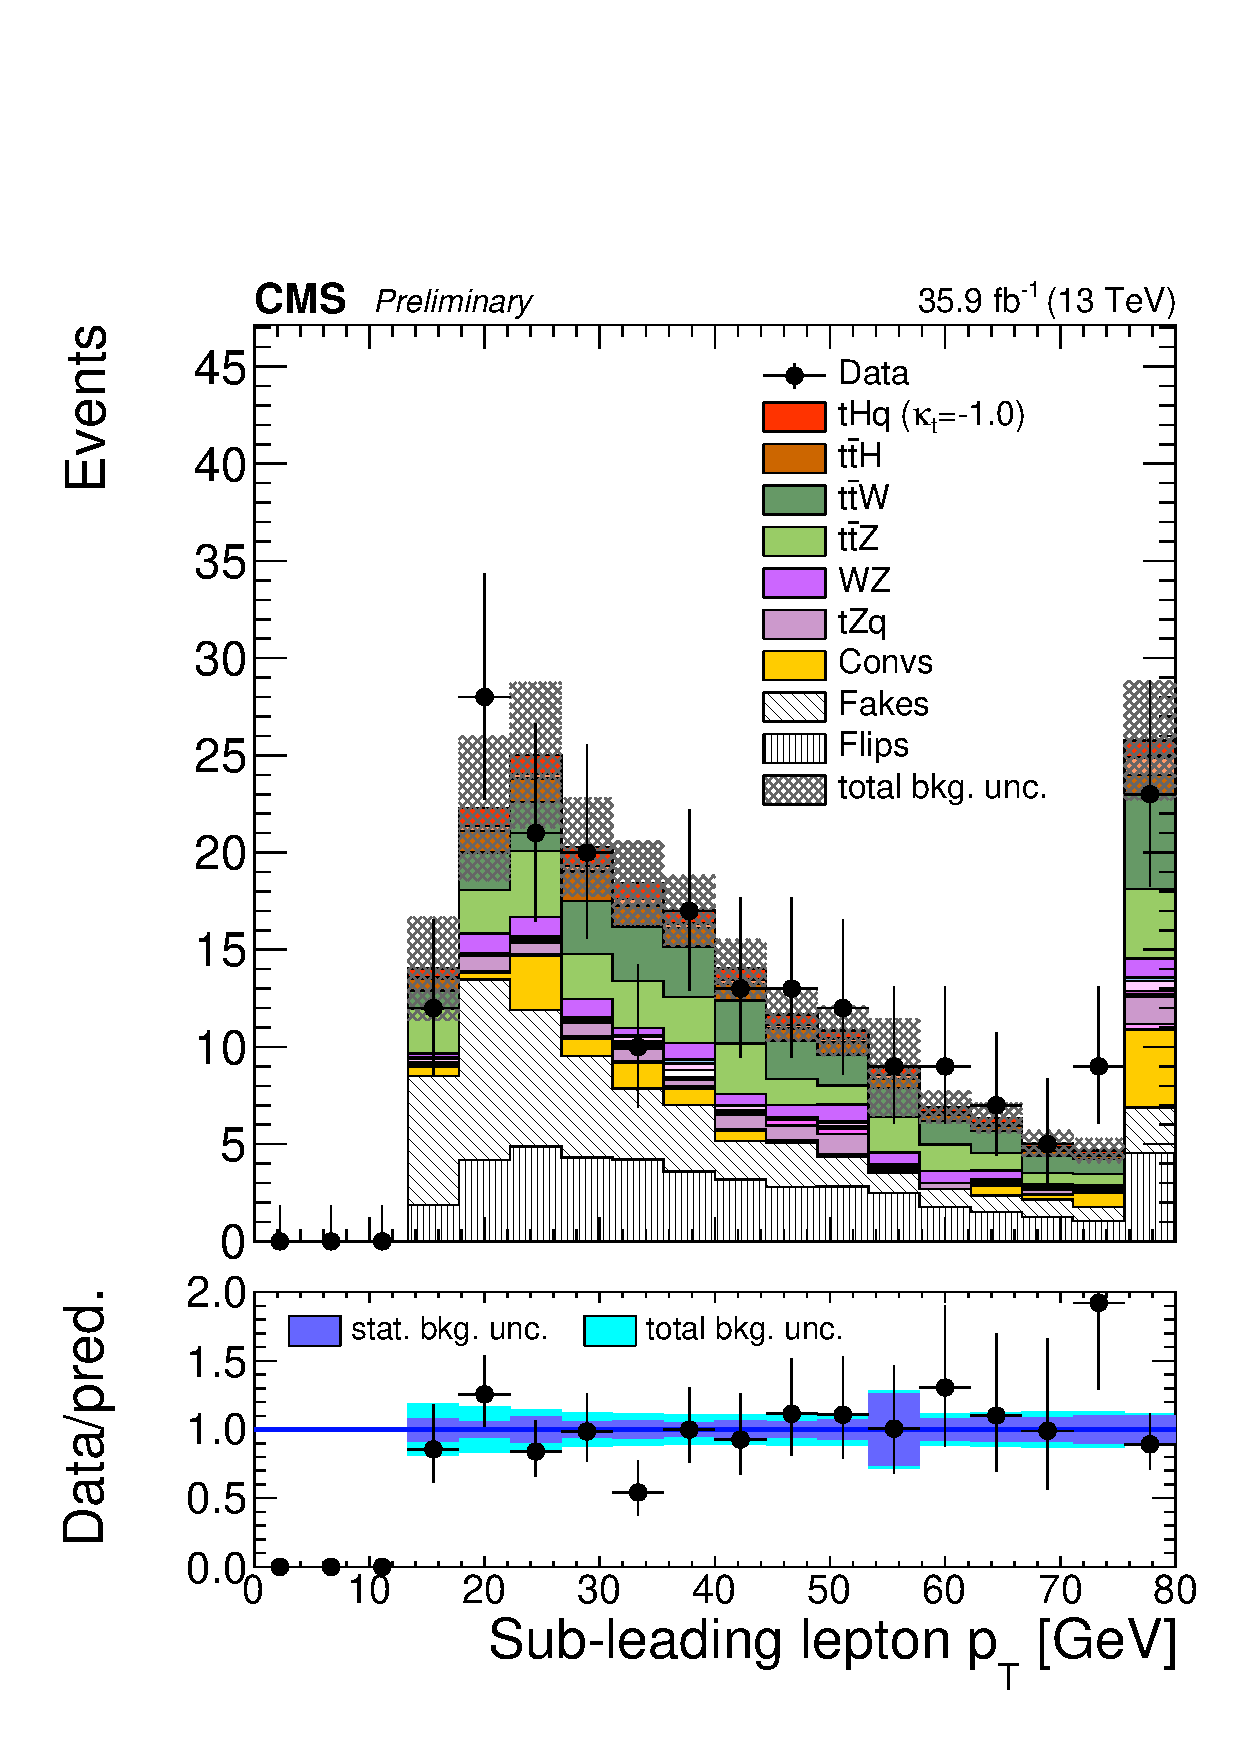
\includegraphics[width=0.22\textwidth]{figures/signalregion_2lss/ee/Lep2Pt.pdf}
  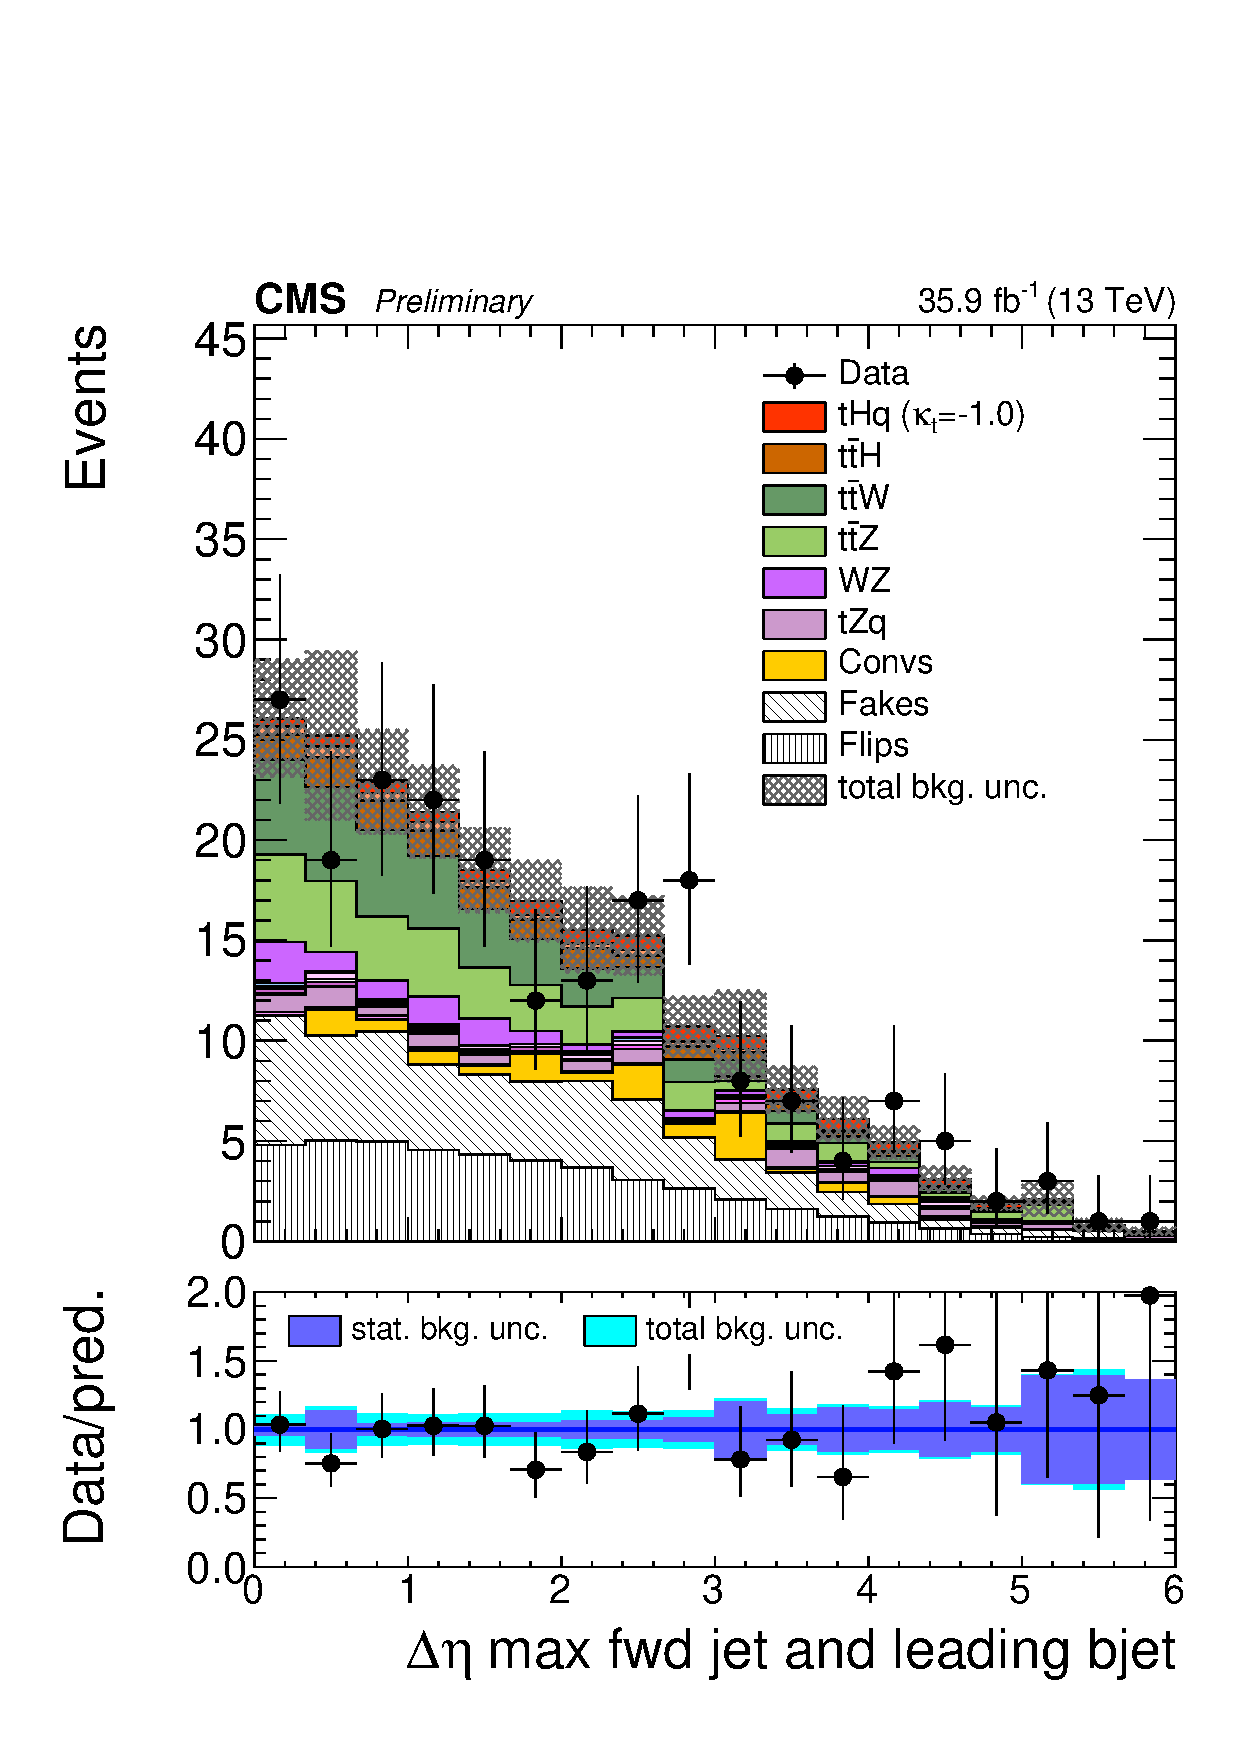
\includegraphics[width=0.22\textwidth]{figures/signalregion_2lss/ee/dEtaFwdJetBJet_40.pdf}
  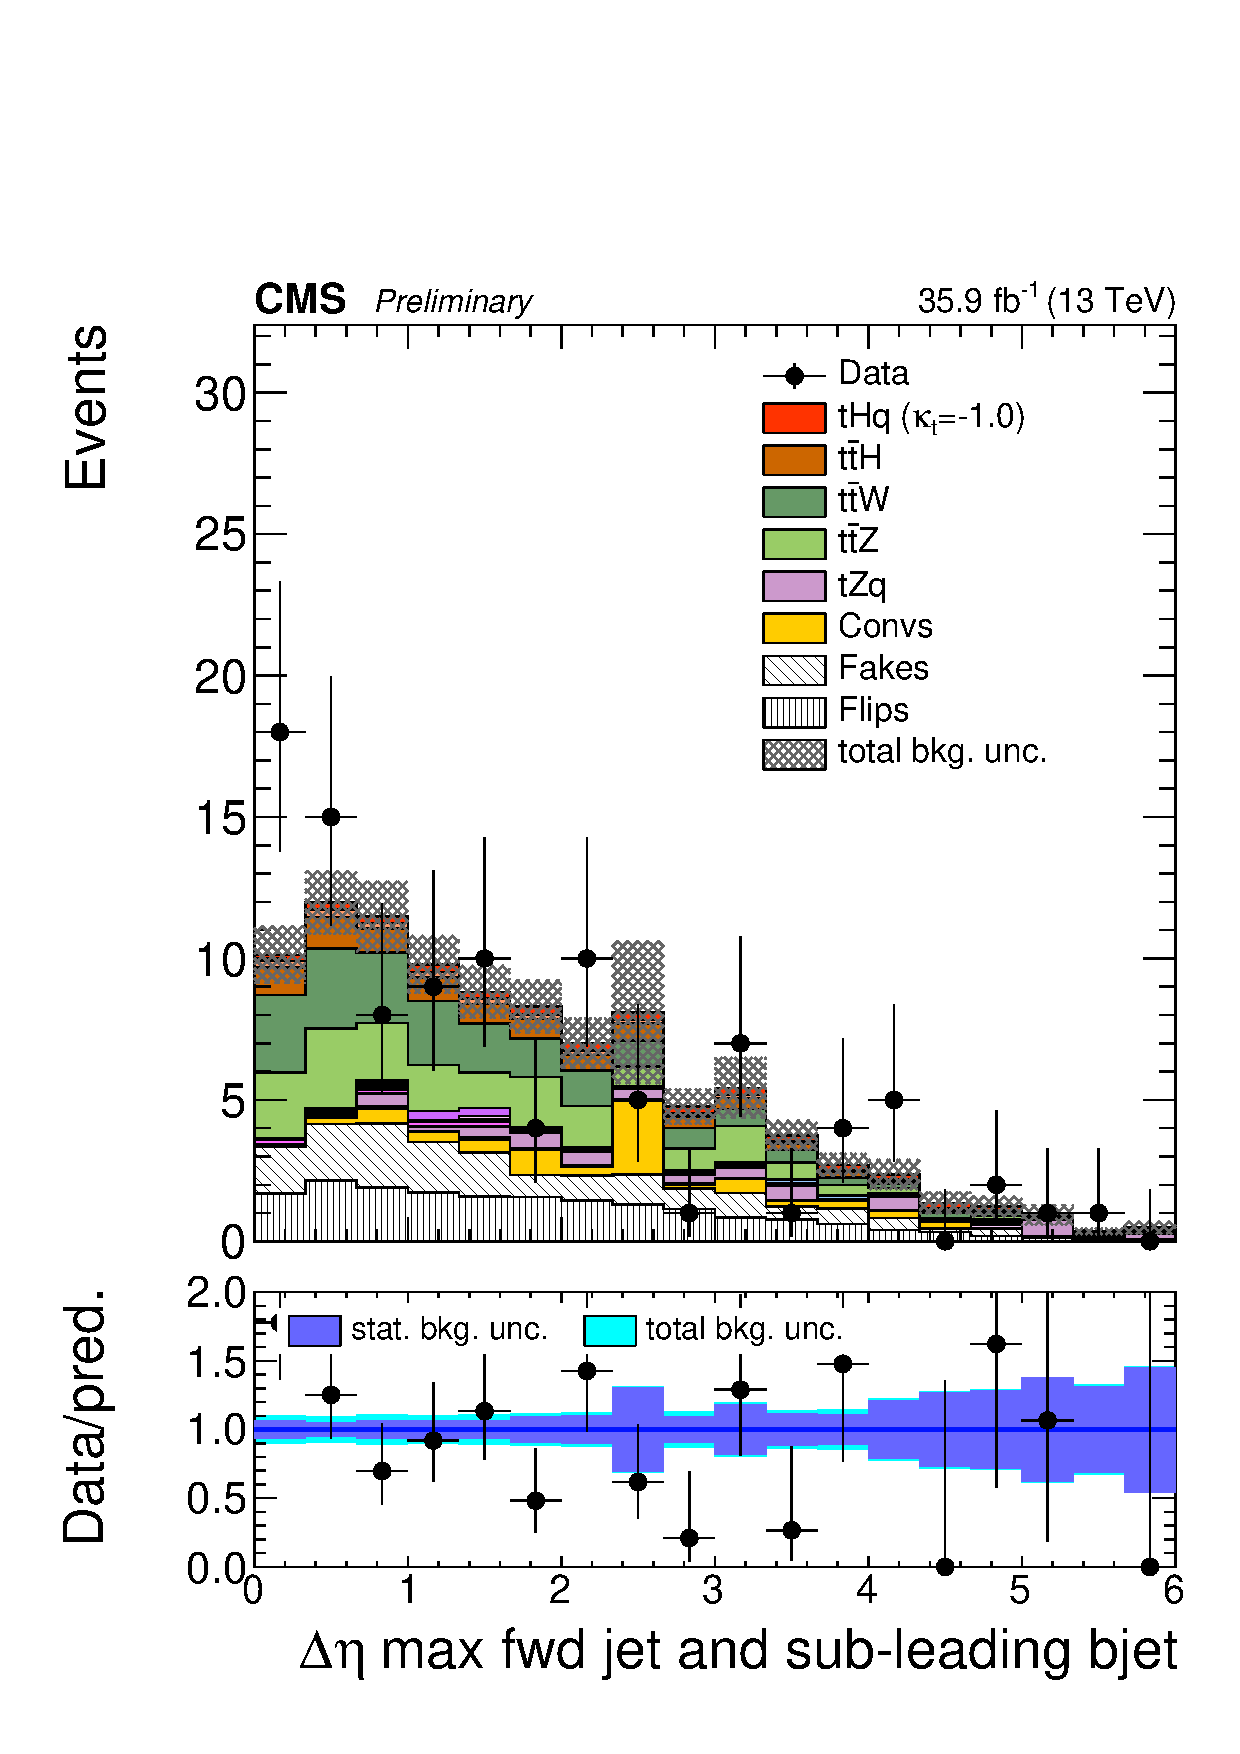
\includegraphics[width=0.22\textwidth]{figures/signalregion_2lss/ee/dEtaFwdJet2BJet_40.pdf}
  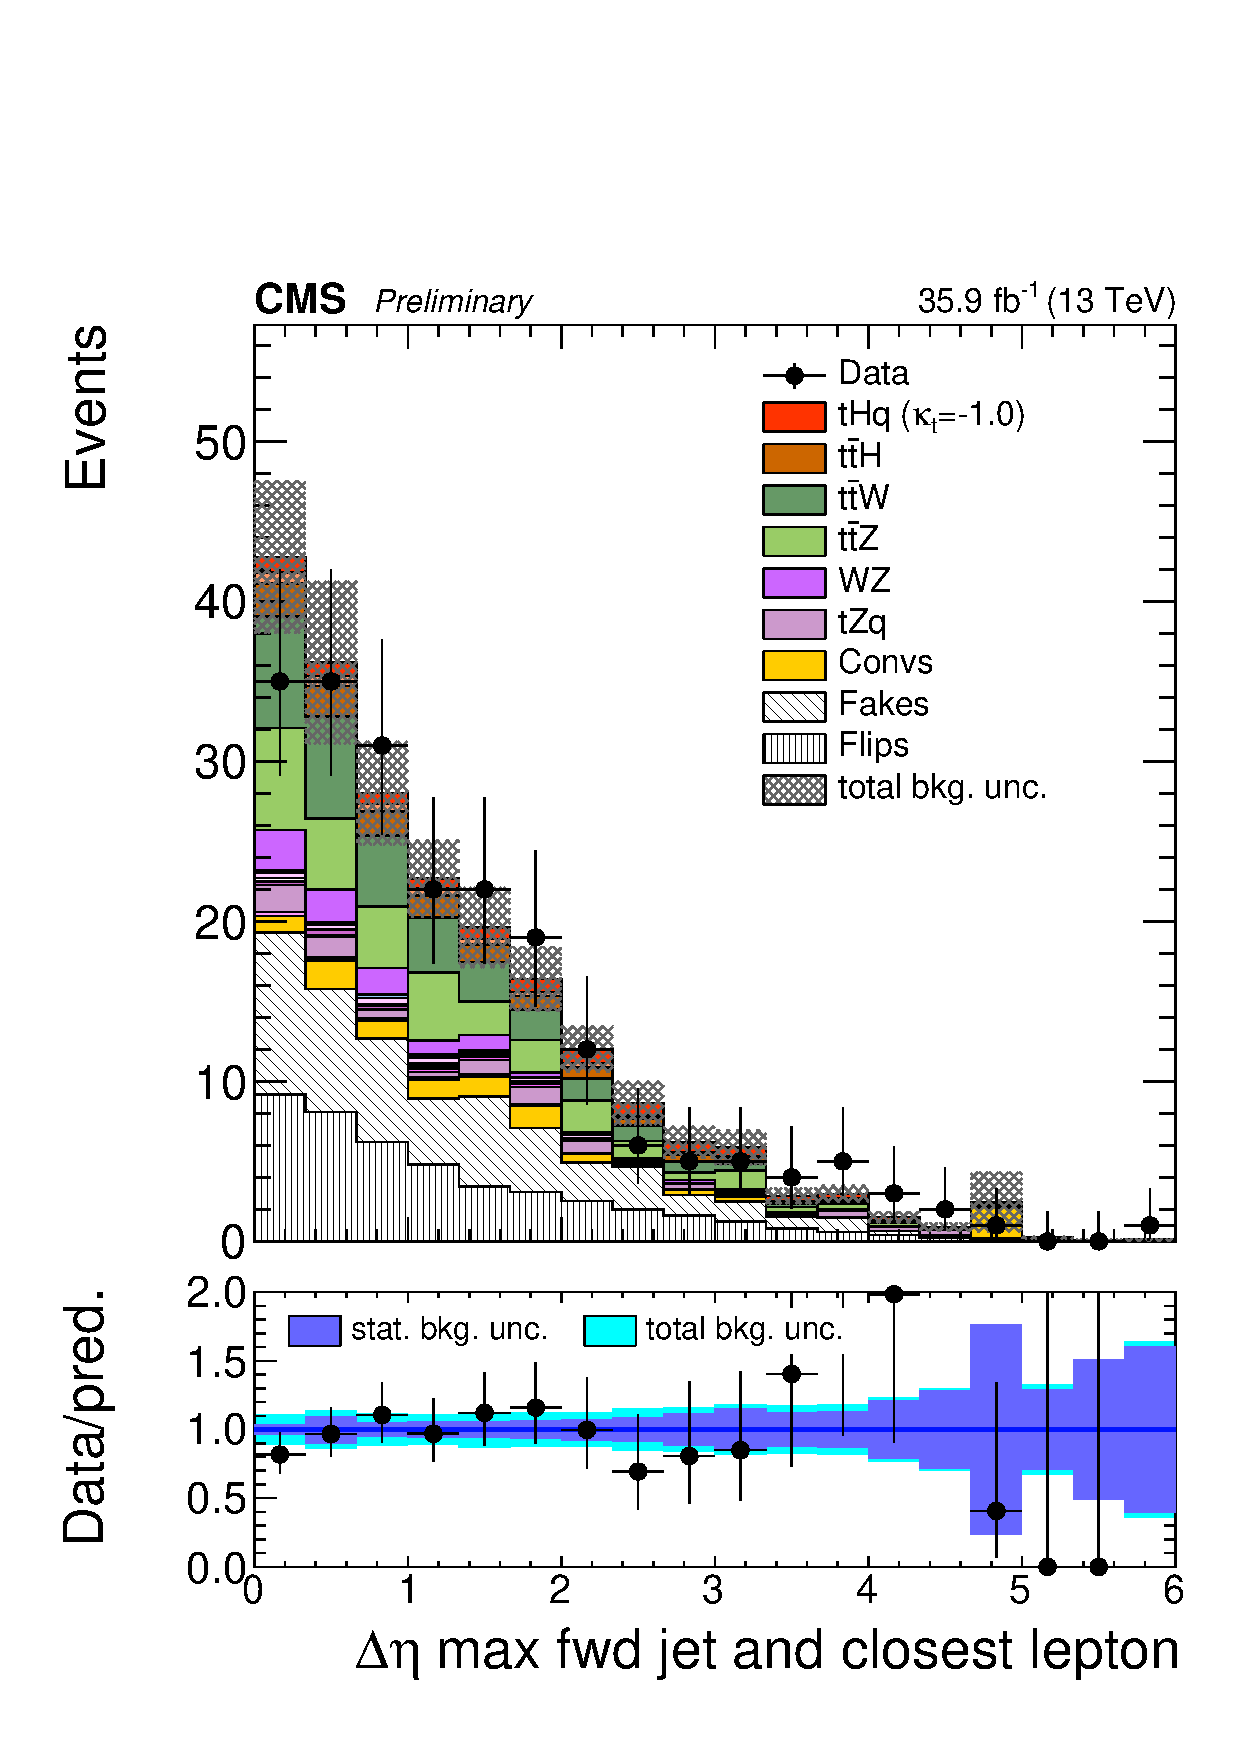
\includegraphics[width=0.22\textwidth]{figures/signalregion_2lss/ee/dEtaFwdJetClosestLep_40.pdf} \\
  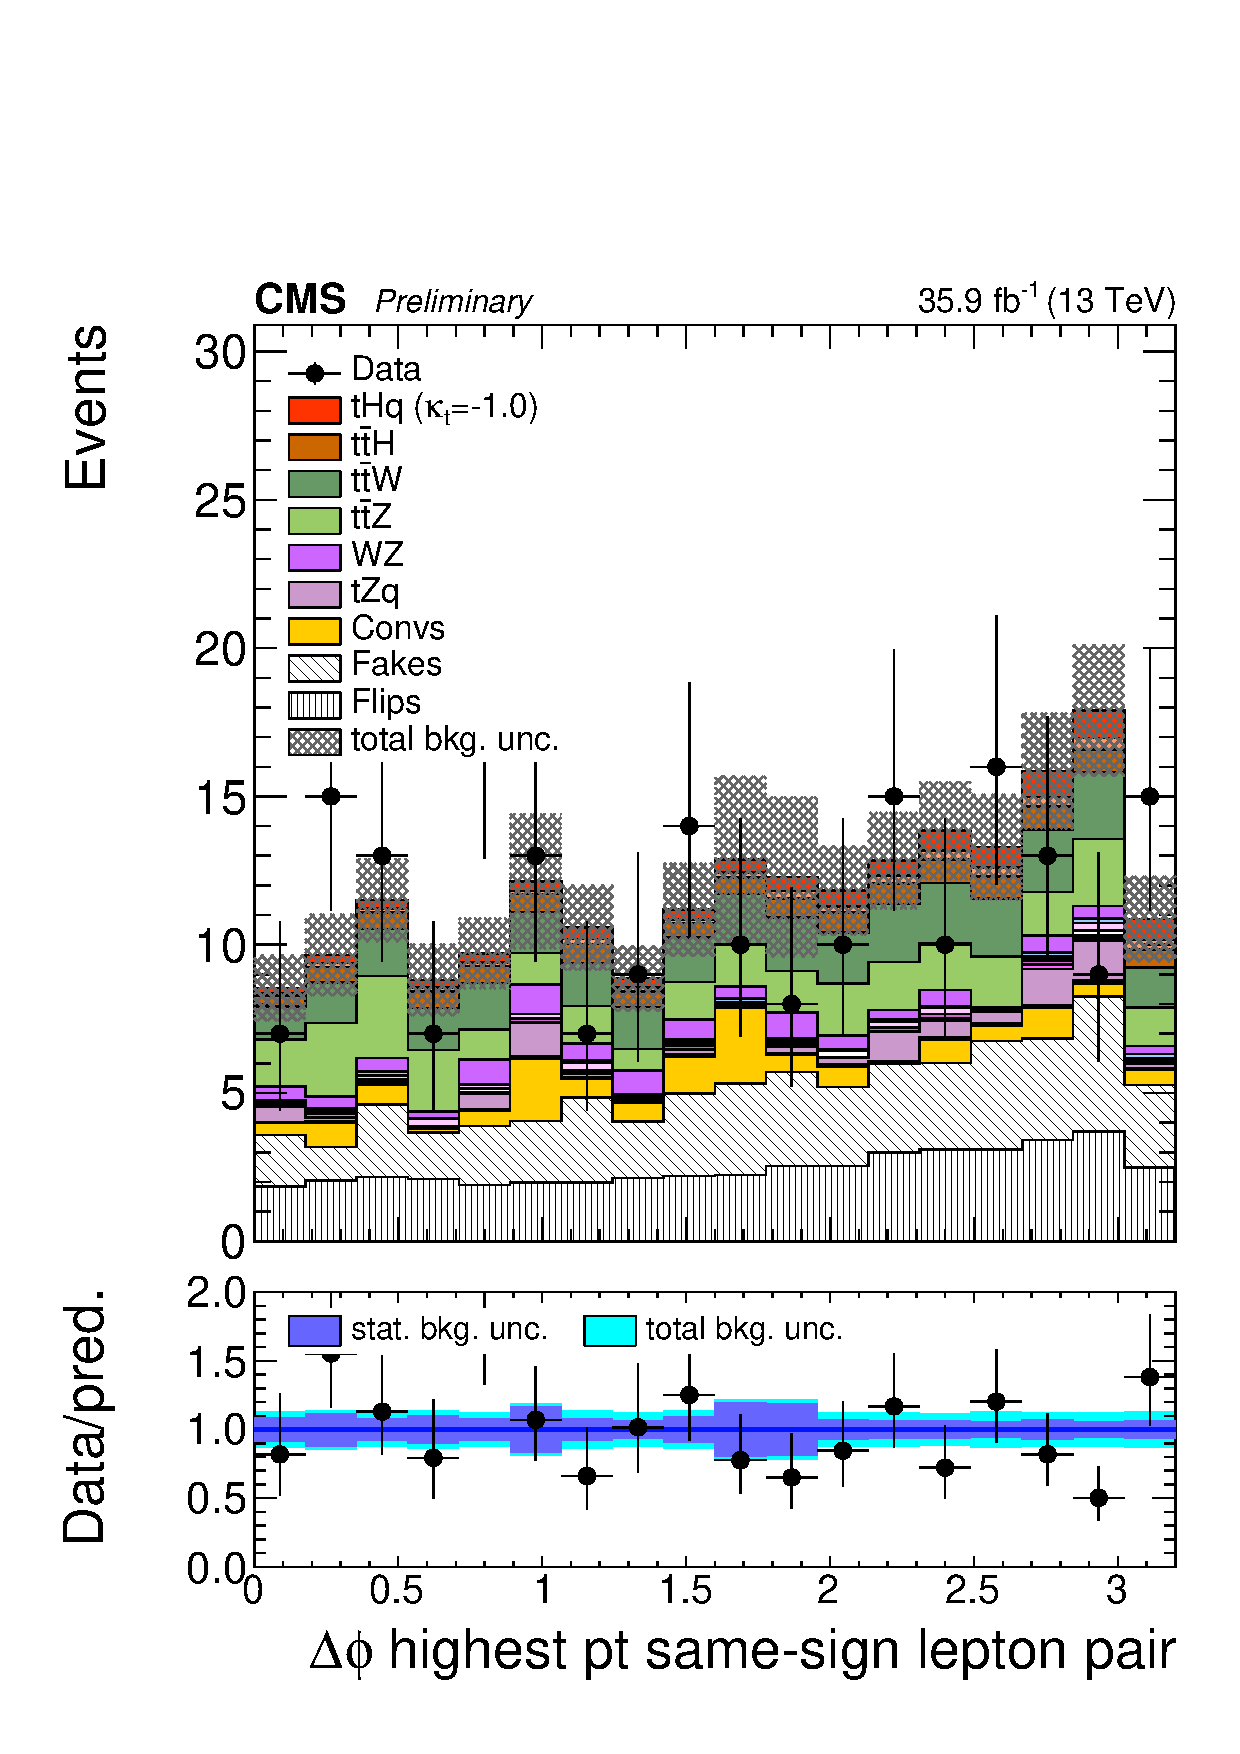
\includegraphics[width=0.22\textwidth]{figures/signalregion_2lss/ee/dPhiHighestPtSSPair.pdf}
  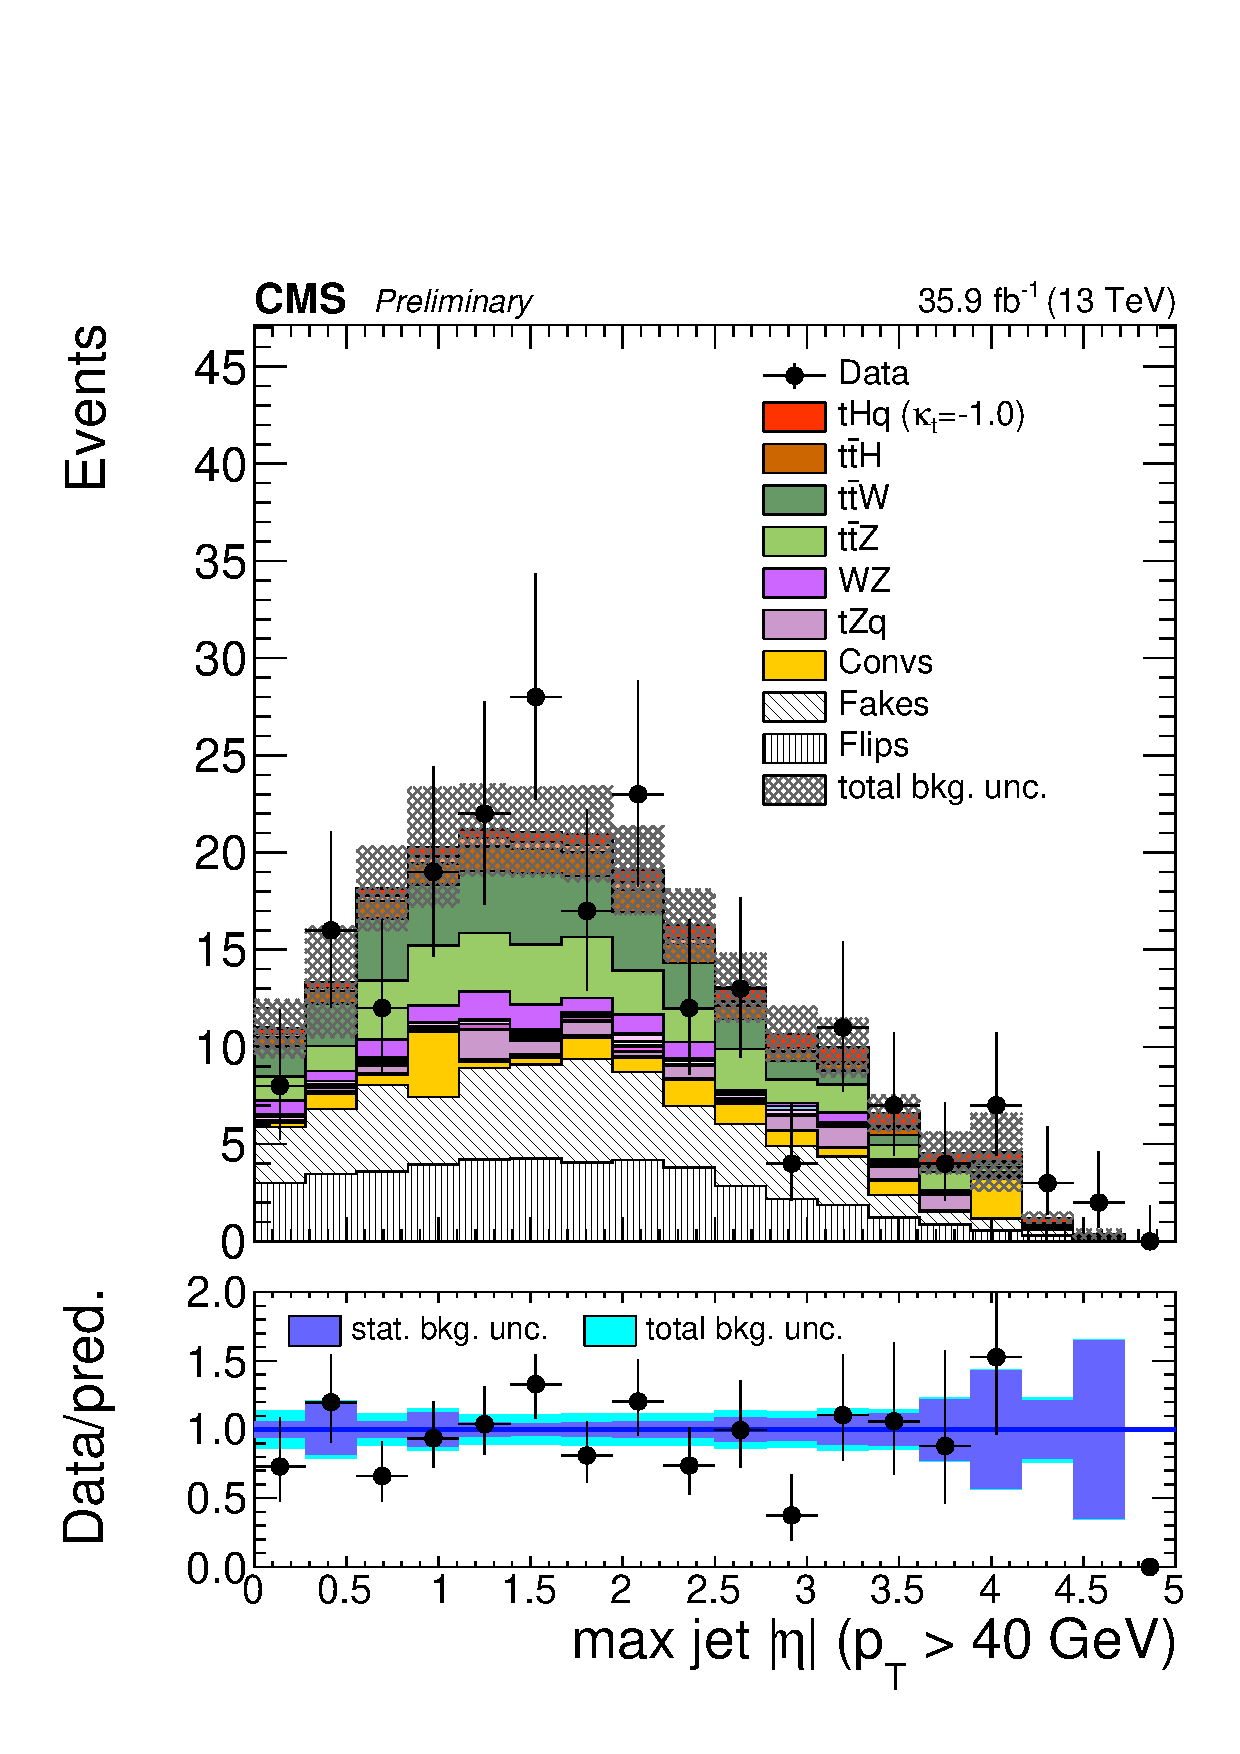
\includegraphics[width=0.22\textwidth]{figures/signalregion_2lss/ee/maxEtaJet25_40.pdf}
  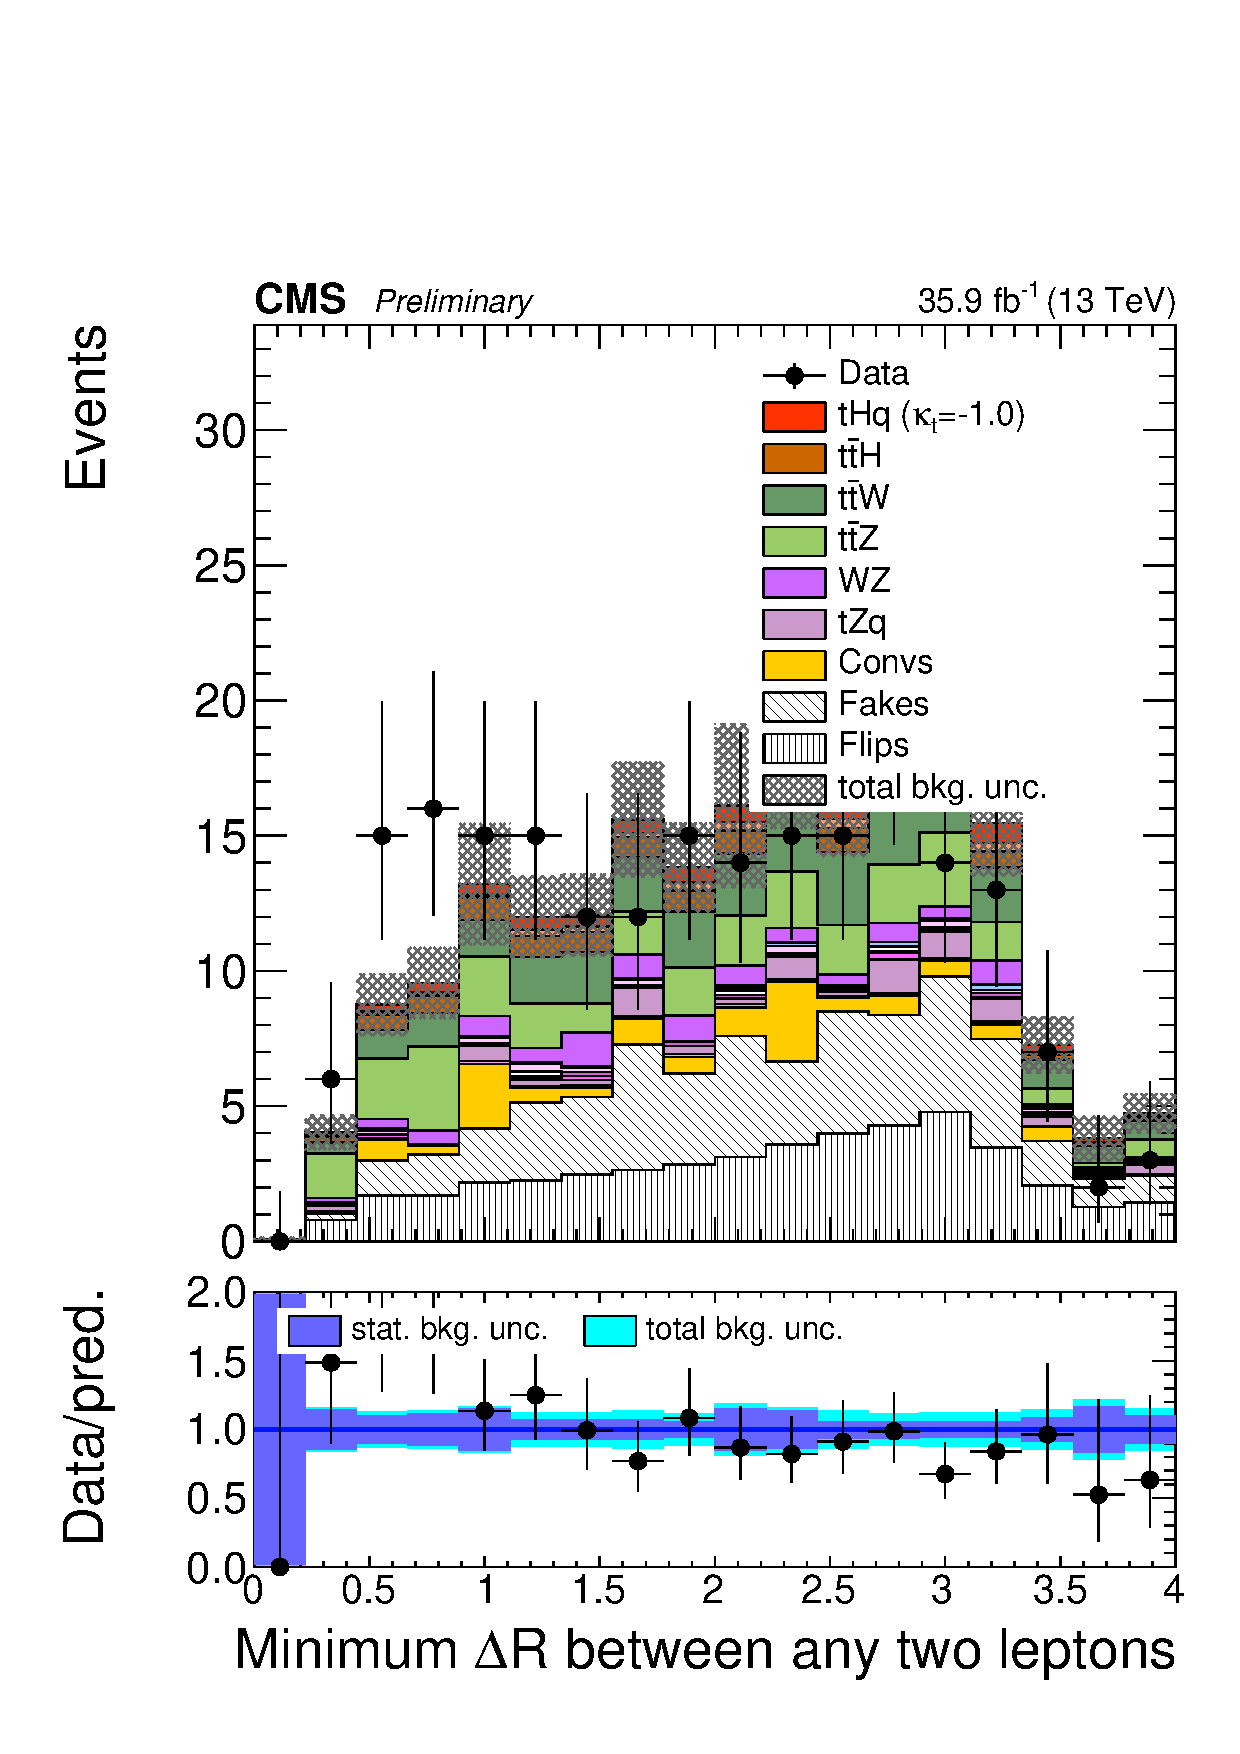
\includegraphics[width=0.22\textwidth]{figures/signalregion_2lss/ee/minDRll.pdf} 
  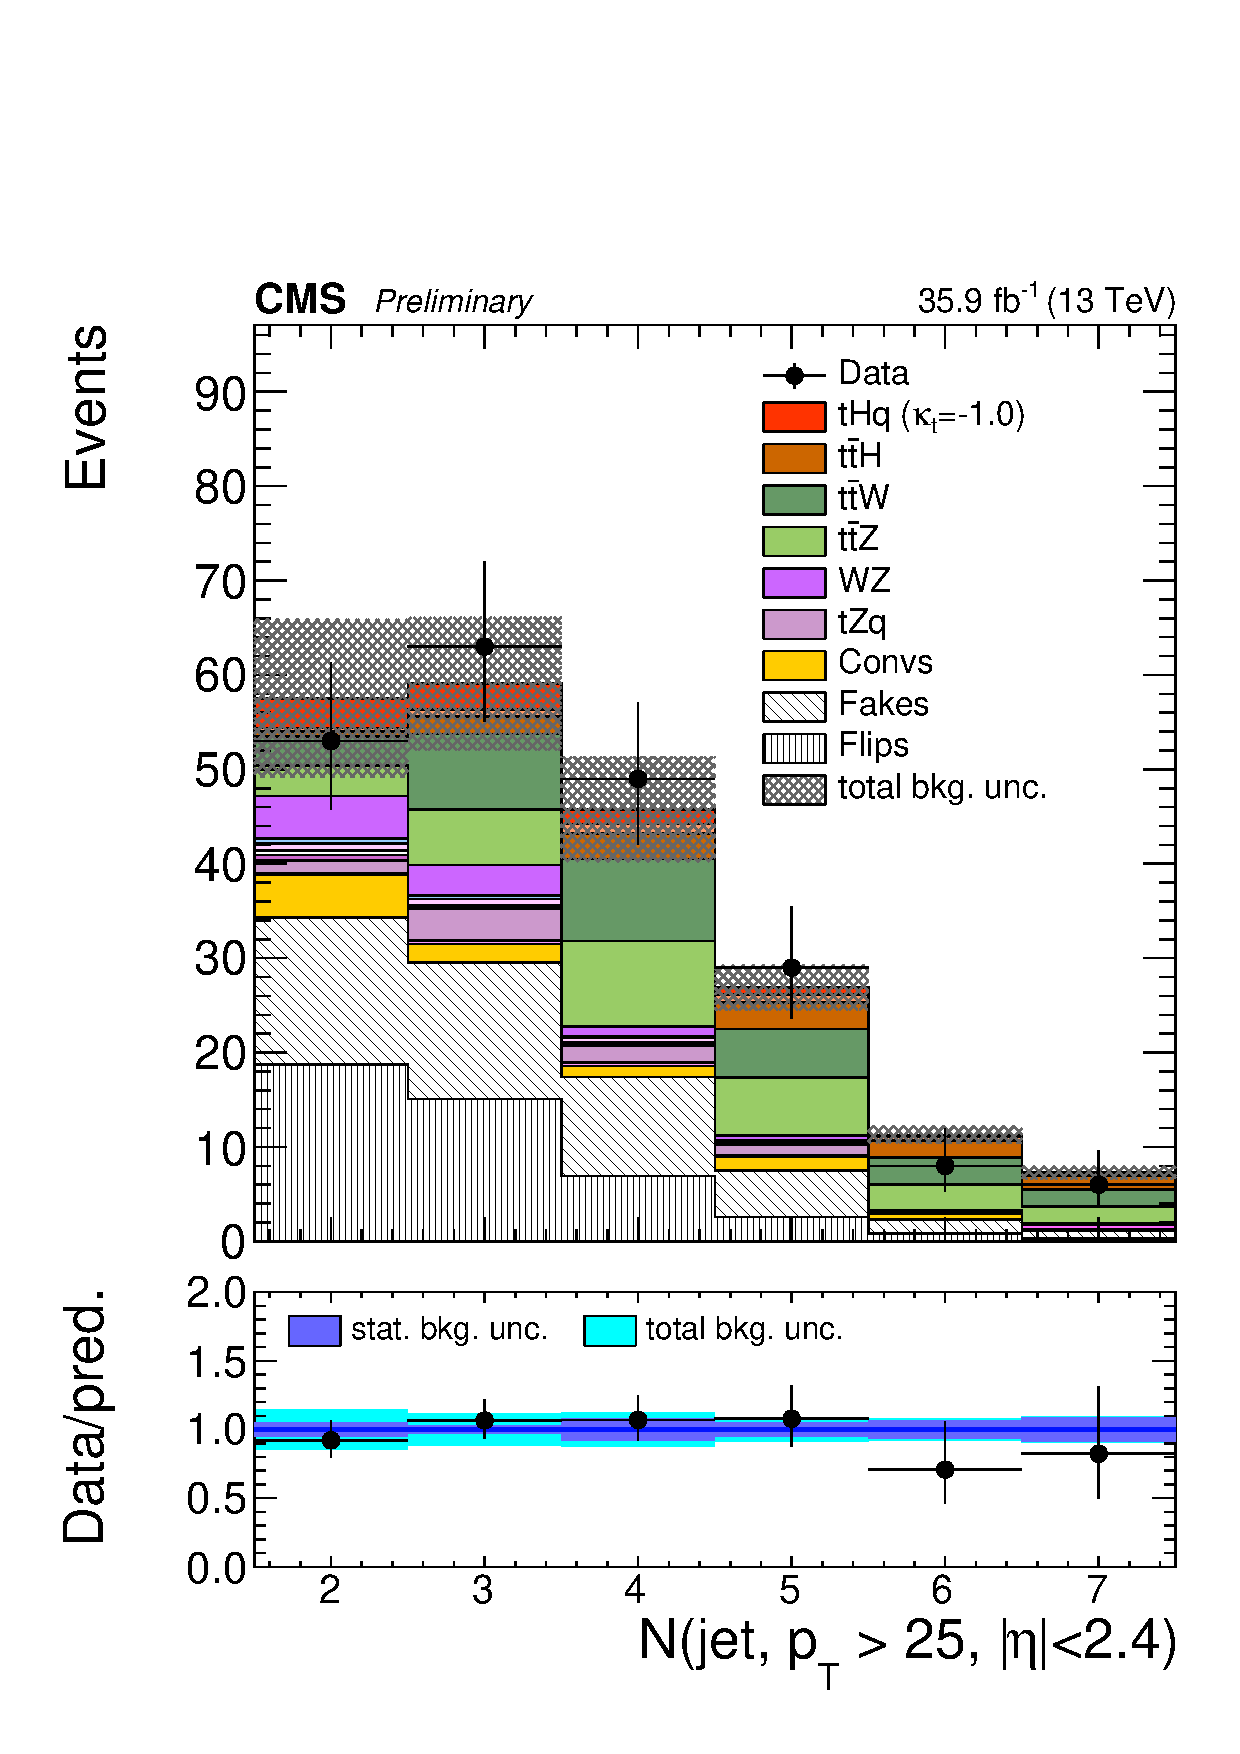
\includegraphics[width=0.22\textwidth]{figures/signalregion_2lss/ee/nJet25.pdf} \\
  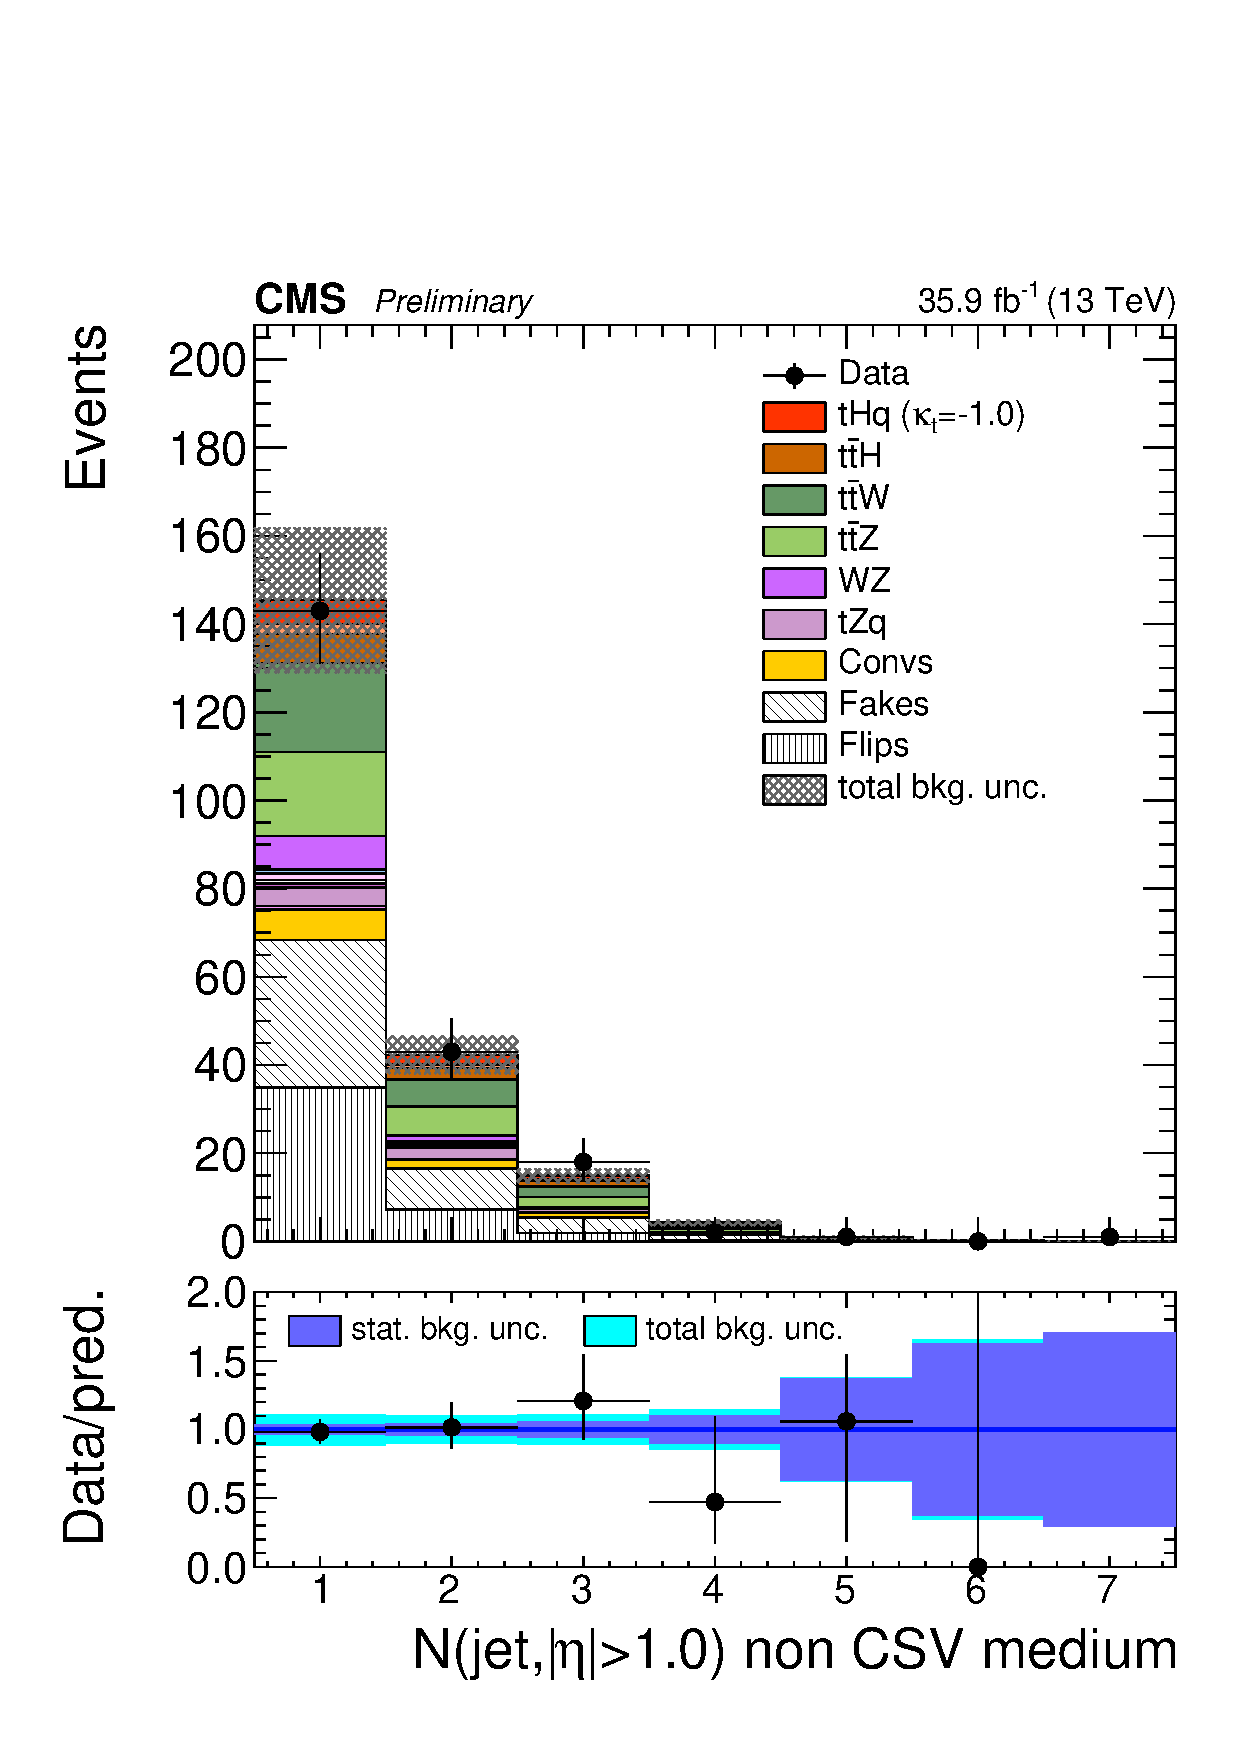
\includegraphics[width=0.22\textwidth]{figures/signalregion_2lss/ee/nJetEta1_40.pdf}
  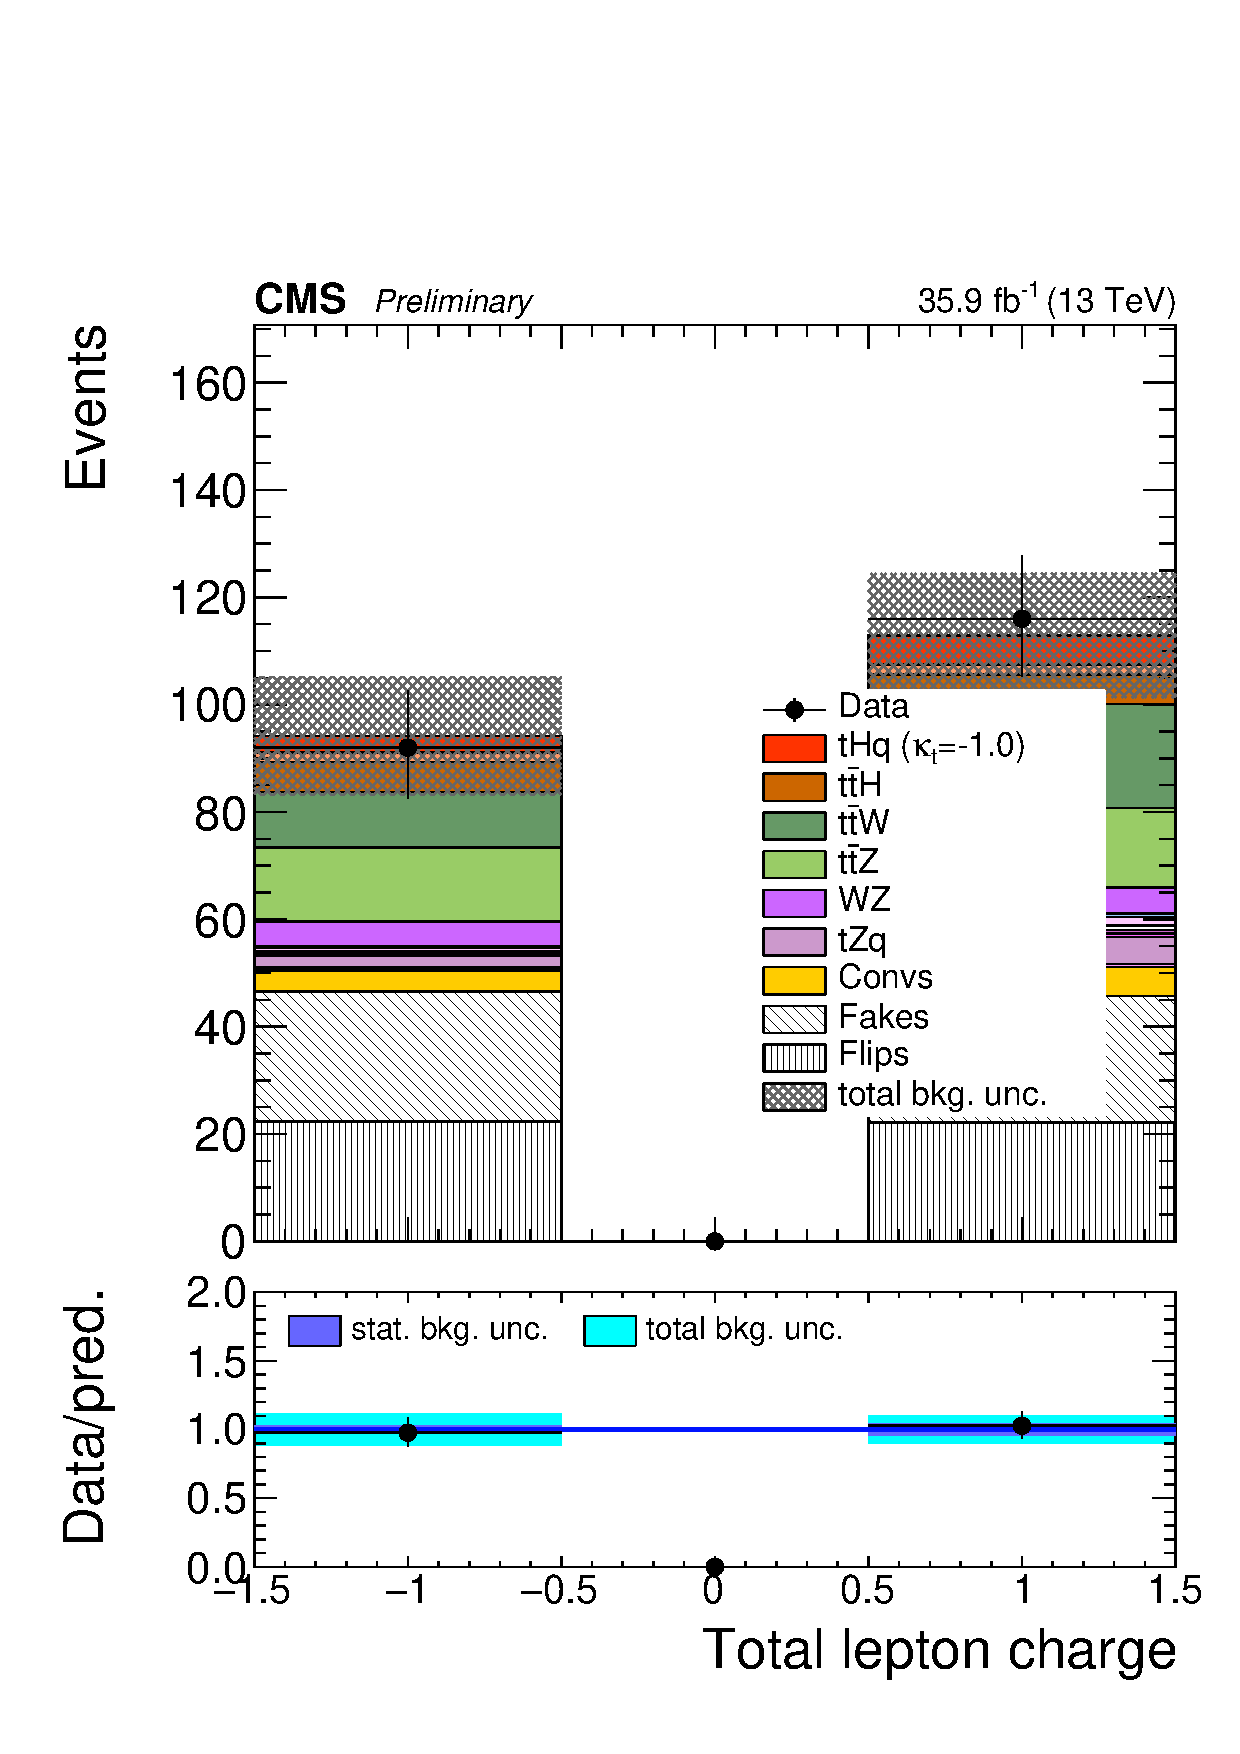
\includegraphics[width=0.22\textwidth]{figures/signalregion_2lss/ee/totCharge.pdf}
\caption{Distributions of input variables to the BDT for signal discrimination, in $\Pe^{\pm}\Pe^{\pm}$ channel, normalized to their cross section and to 35.9\fbinv.}
\label{fig:input_vars_2lss_xsec_ee}
\end{figure}


\clearpage

\section{Signal discrimination}
\label{sec:sigdisc}
The \tHq\ signal is separated from the main backgrounds using a boosted decision tree (BDT) classifier, trained on simulated signal and background events.
A set of discriminating variables are given as input to the BDT which produces a output distribution maximizing the discrimination power.
Table~\ref{tab:bdtinputs} lists the input variables used while Figures~\ref{fig:input_vars_3l} and~\ref{fig:input_vars_2lss} show their distributions for the relevant signal and background samples, for the three lepton and same-sign dilepton channels, respectively.
The same or equivalent input variables are found to be performing well for both three lepton and same-sign dilepton channels.

Two BDT classifiers are trained for the two main backgrounds expected in the analysis: events with prompt leptons from \ttW\ and \ttZ\ (also referred to as \ttV), and events with non-prompt leptons from \ttbar.
The datasets used in the training are the \tHq\ signal (see Tab.~\ref{tab:sigsamples}), and LO \MADGRAPH\ samples of \ttW\ and \ttZ, in an admixture proportional to their respective cross sections (see Tab.~\ref{tab:ttvlo_samples}).

\begin{table}[h!]
\centering
\begin{tabular}{lp{10cm}}
Variable name        & Description\\ \hline
nJet25               & Number of jets with $\pt>25\GeV$, $|\eta|<2.4$\\
MaxEtaJet25          & Maximum $|\eta|$ of any (non-CSV-loose) jet with $\pt>25\GeV$\\
% nBJetLoose25         & Number of jets with $\pt>25\GeV$, CSV loose\\
totCharge            & Sum of lepton charges \\
nJetEta1             & Number of jets with $|\eta|>1.0$, non-CSV-loose\\
detaFwdJetBJet       & $\Delta \eta$ between forward light jet and hardest CSV loose jet\\
detaFwdJet2BJet      & $\Delta \eta$ between forward light jet and second hardest CSV loose jet (defaults to -1 in events with only one CSV loose jet) \\
detaFwdJetClosestLep & $\Delta \eta$ between forward light jet and closest lepton\\
dphiHighestPtSSPair  & $\Delta \phi$ of highest \pt\ same-sign lepton pair\\
minDRll              & minimum $\Delta R$ between any two leptons\\
Lep3Pt/Lep2Pt        & \pt\ of the $3^{rd}$ lepton ($2^{nd}$ for ss2l)\\ \hline
\end{tabular}
\caption{MVA input discriminating variables}
\label{tab:bdtinputs}
\end{table}


\begin{figure} [!h]
 \centering
 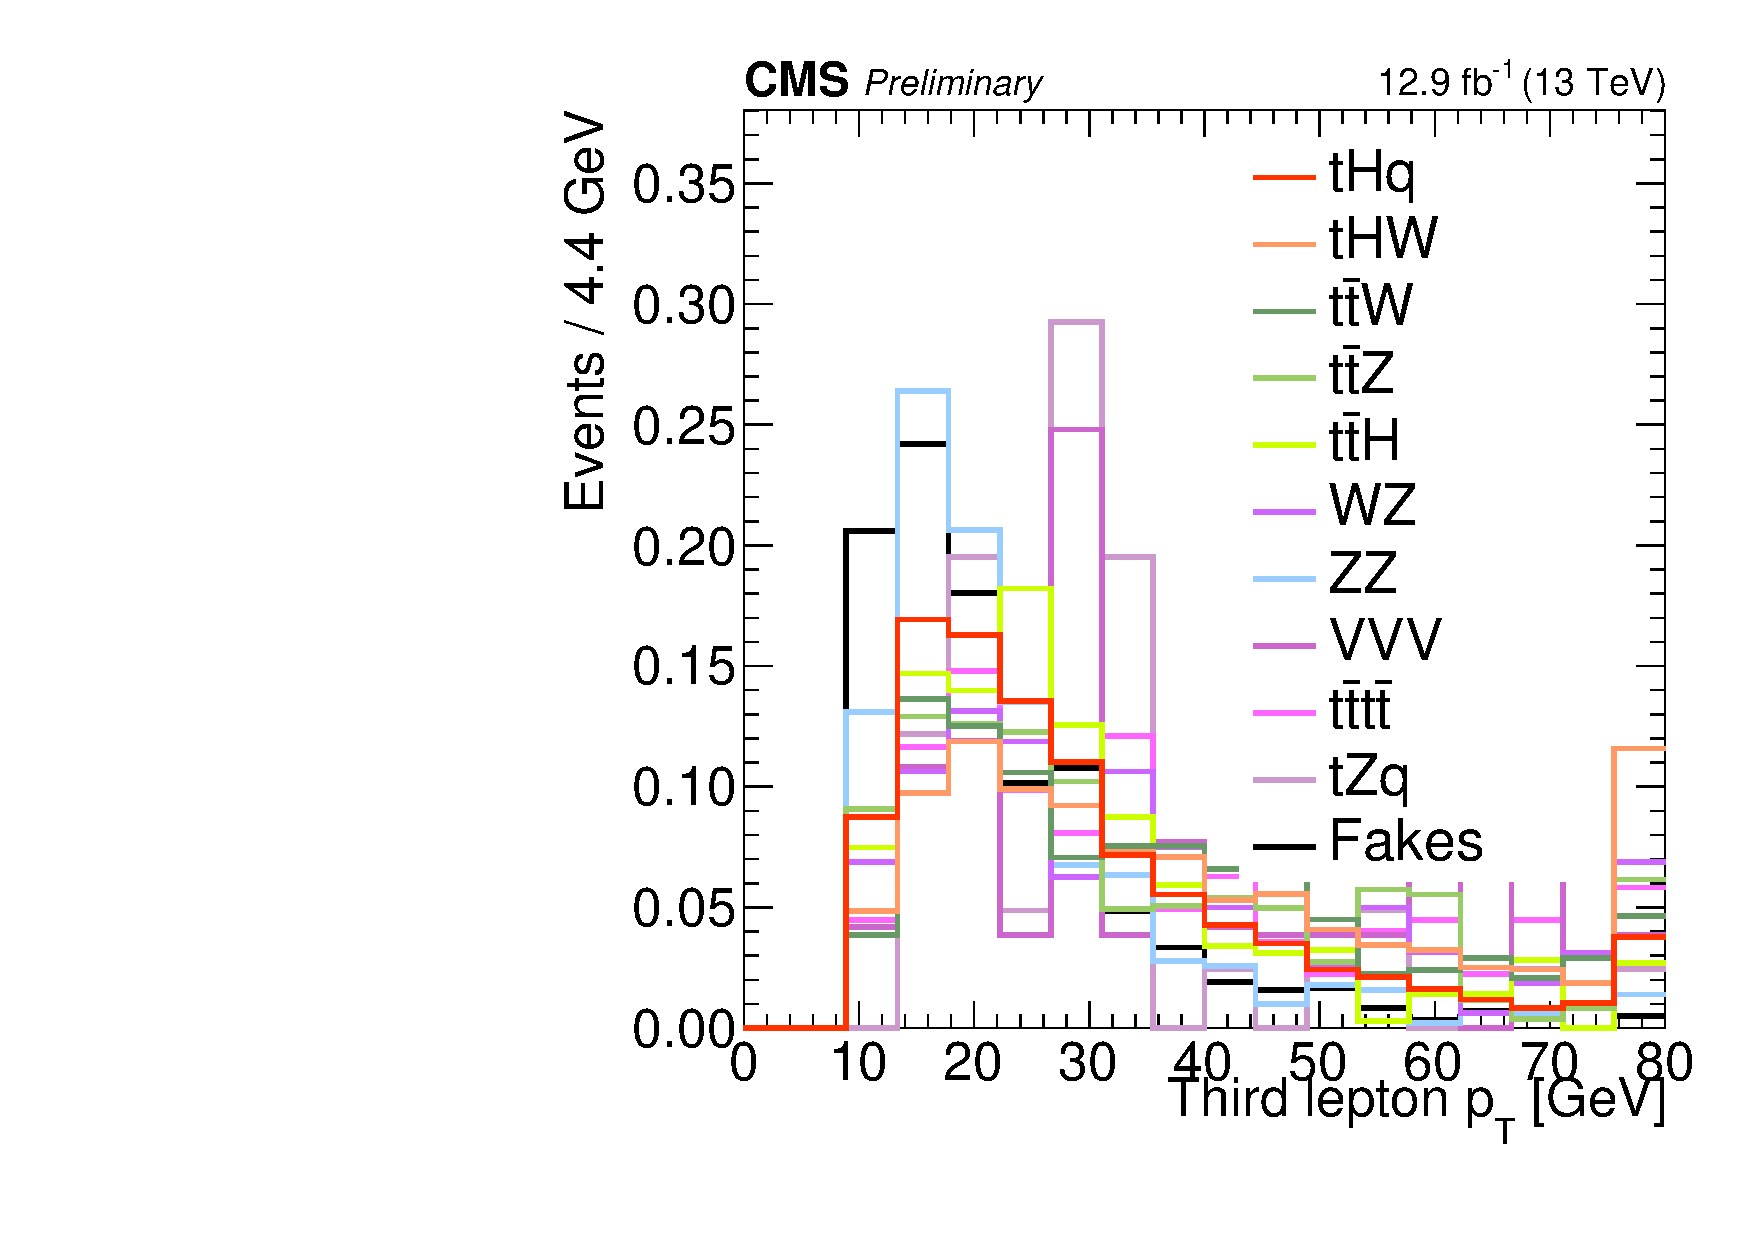
\includegraphics[width=0.245\textwidth]{figures/Lep3Pt.pdf} 
 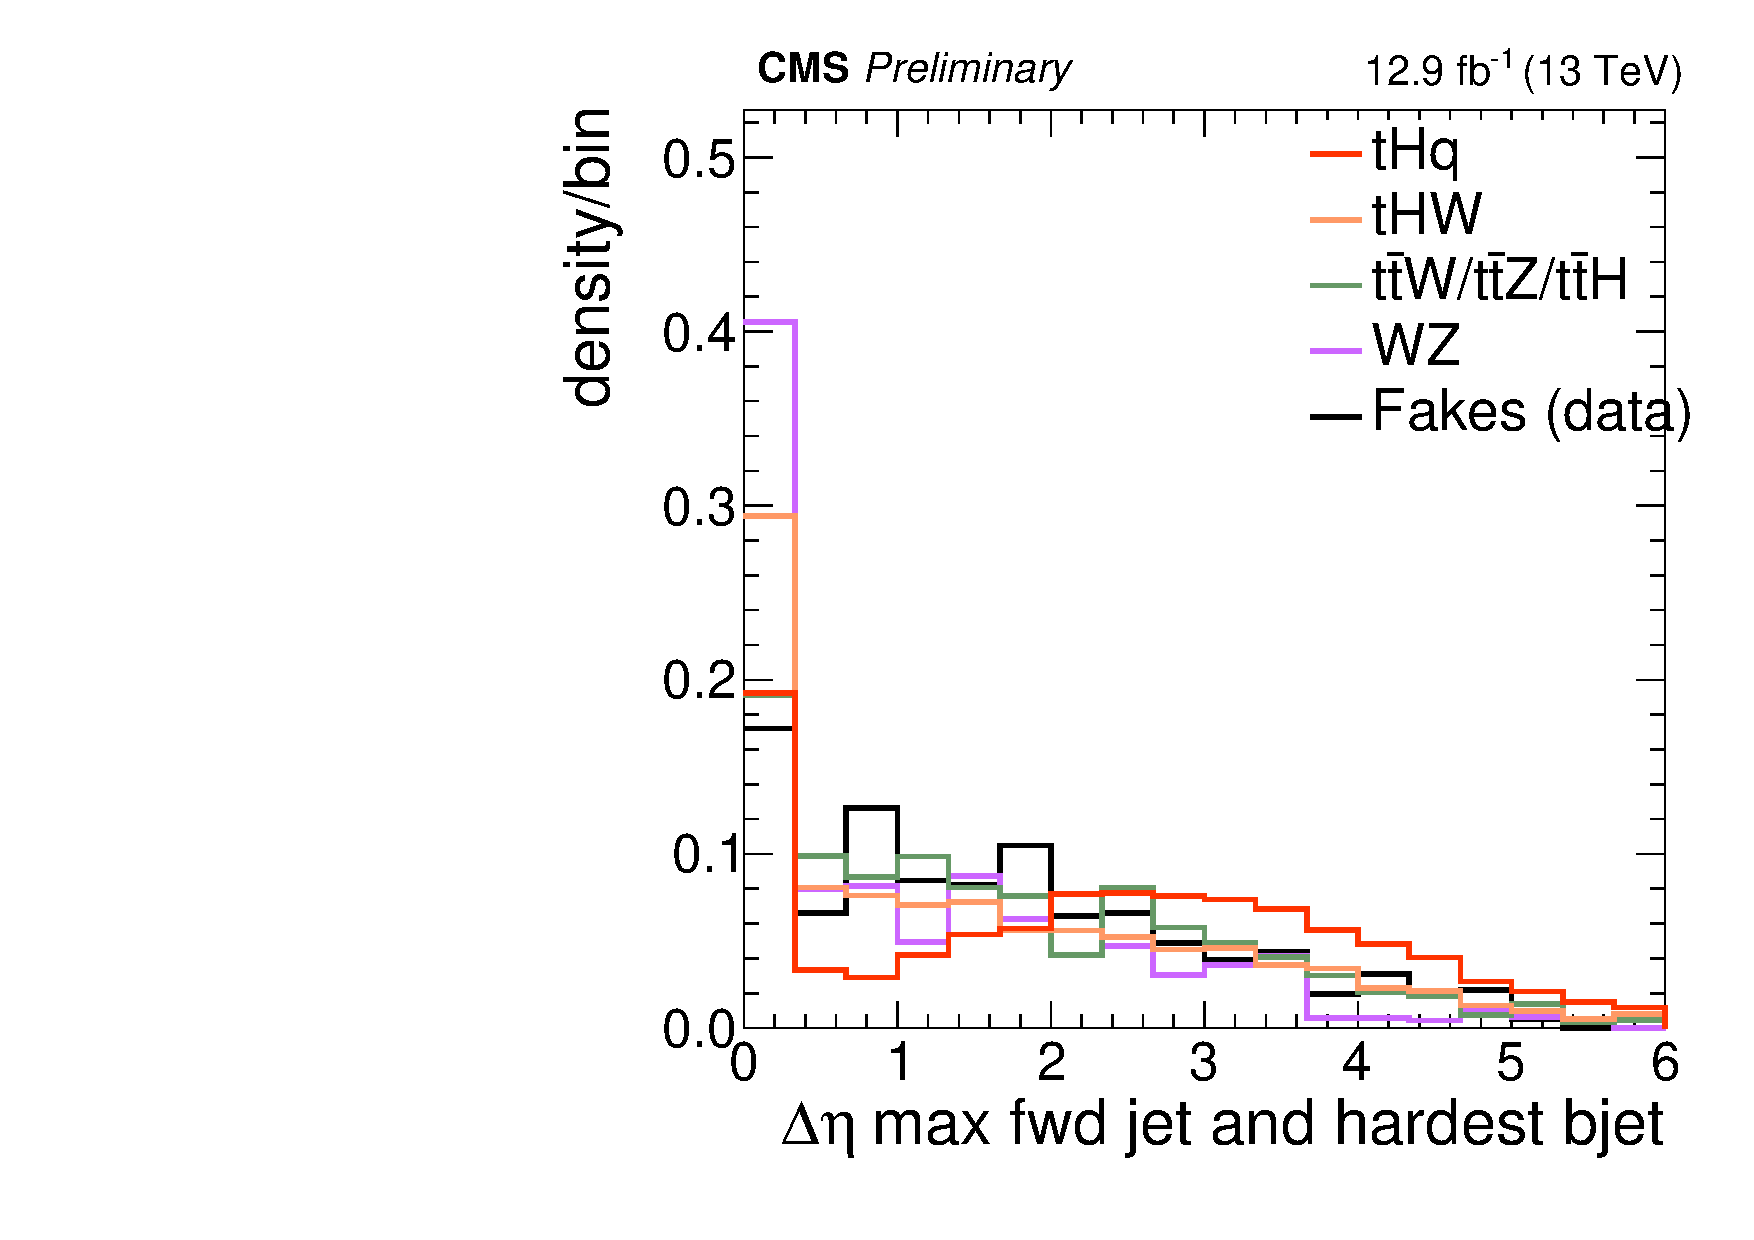
\includegraphics[width=0.245\textwidth]{figures/dEtaFwdJetBJet.pdf}
 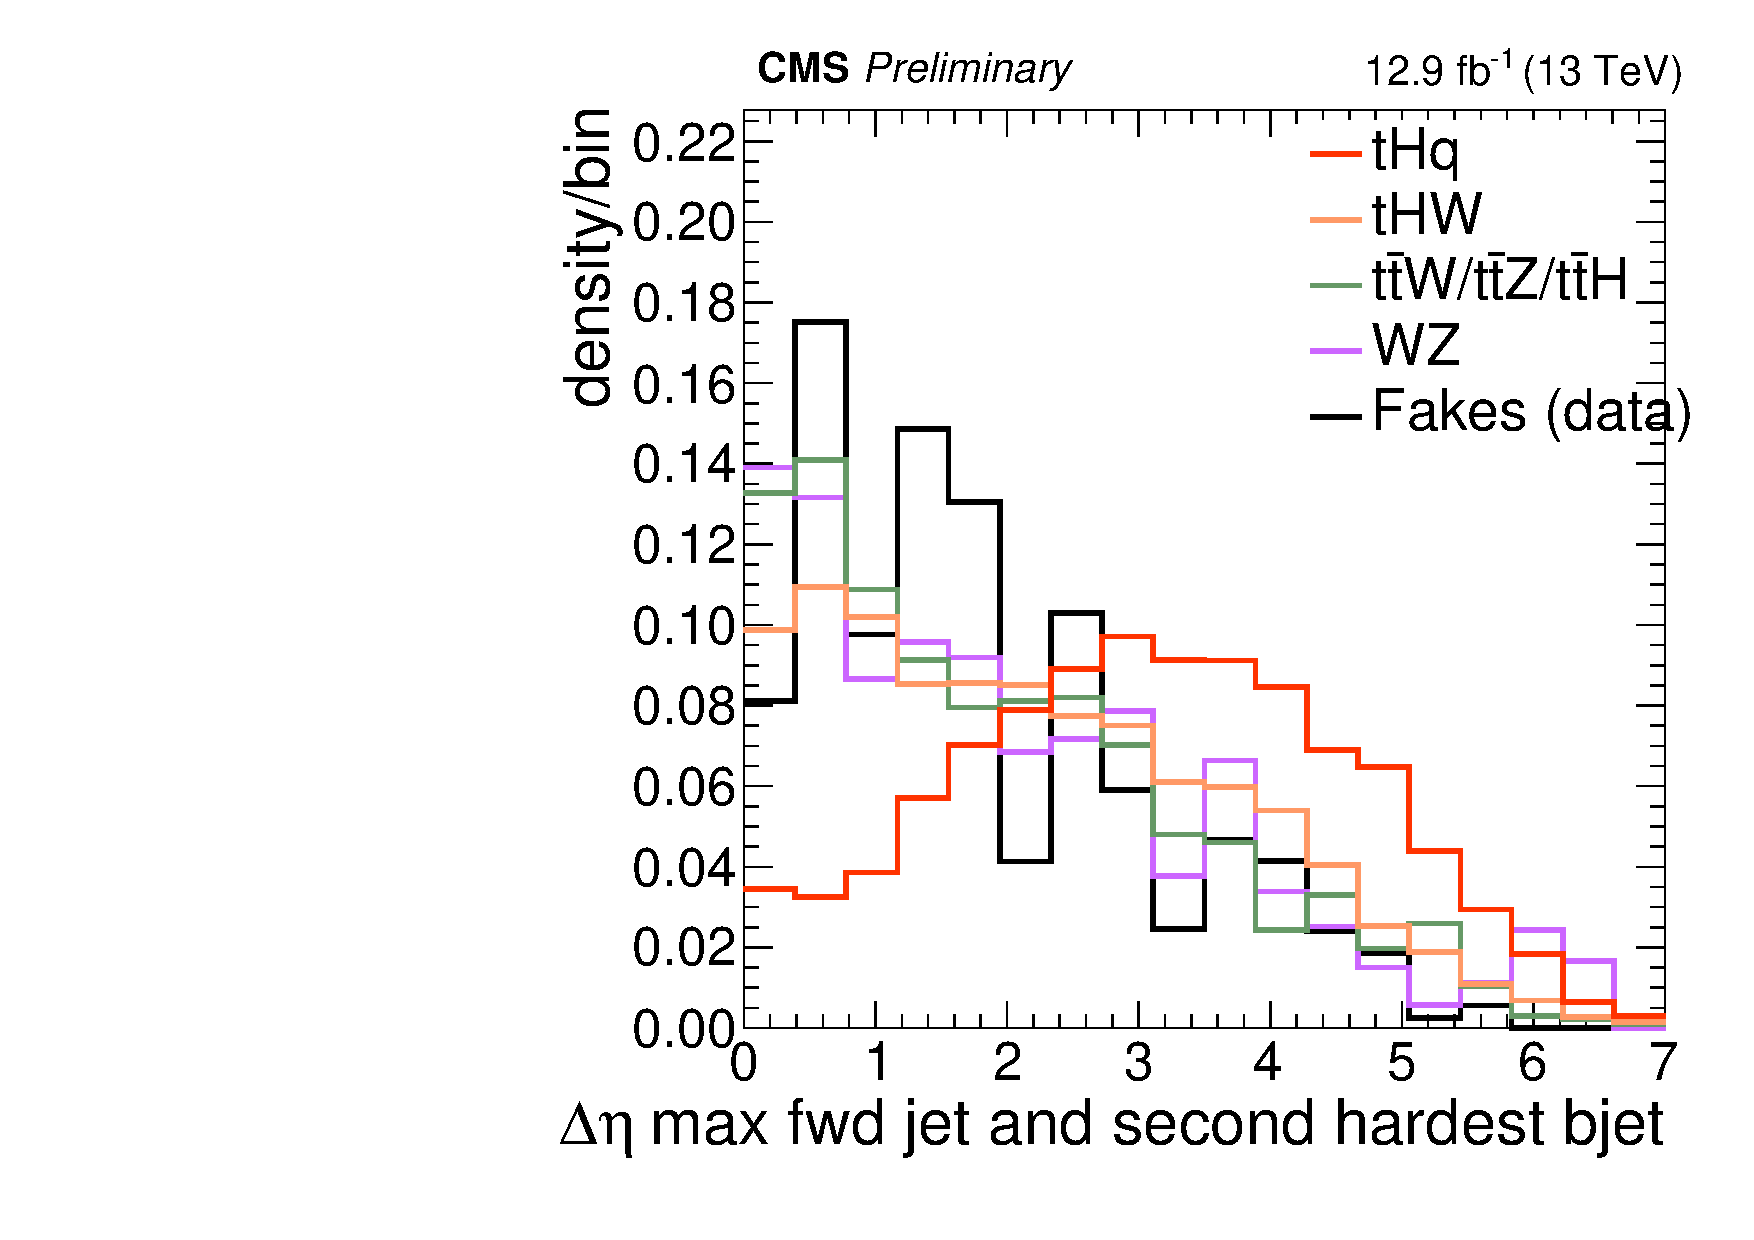
\includegraphics[width=0.245\textwidth]{figures/dEtaFwdJet2BJet.pdf}
 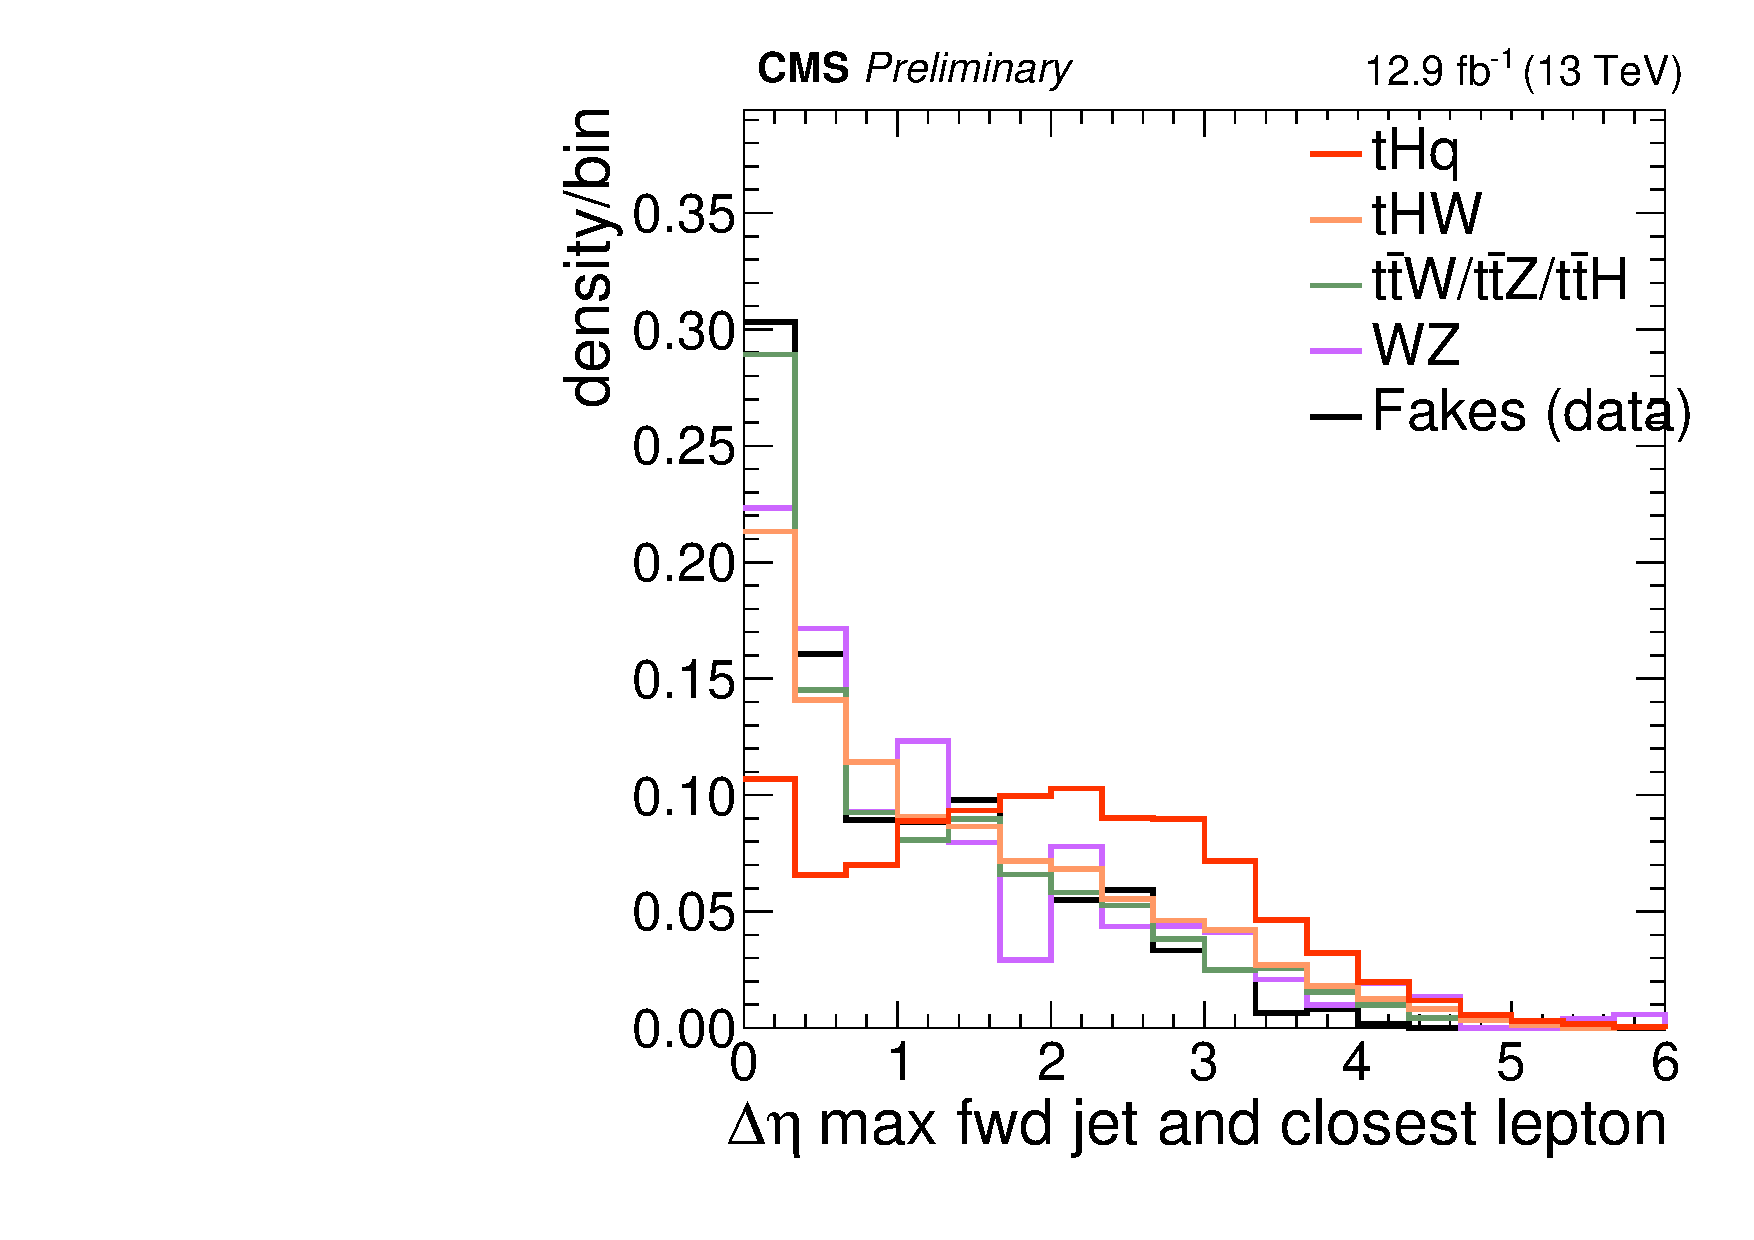
\includegraphics[width=0.245\textwidth]{figures/dEtaFwdJetClosestLep.pdf} \\
 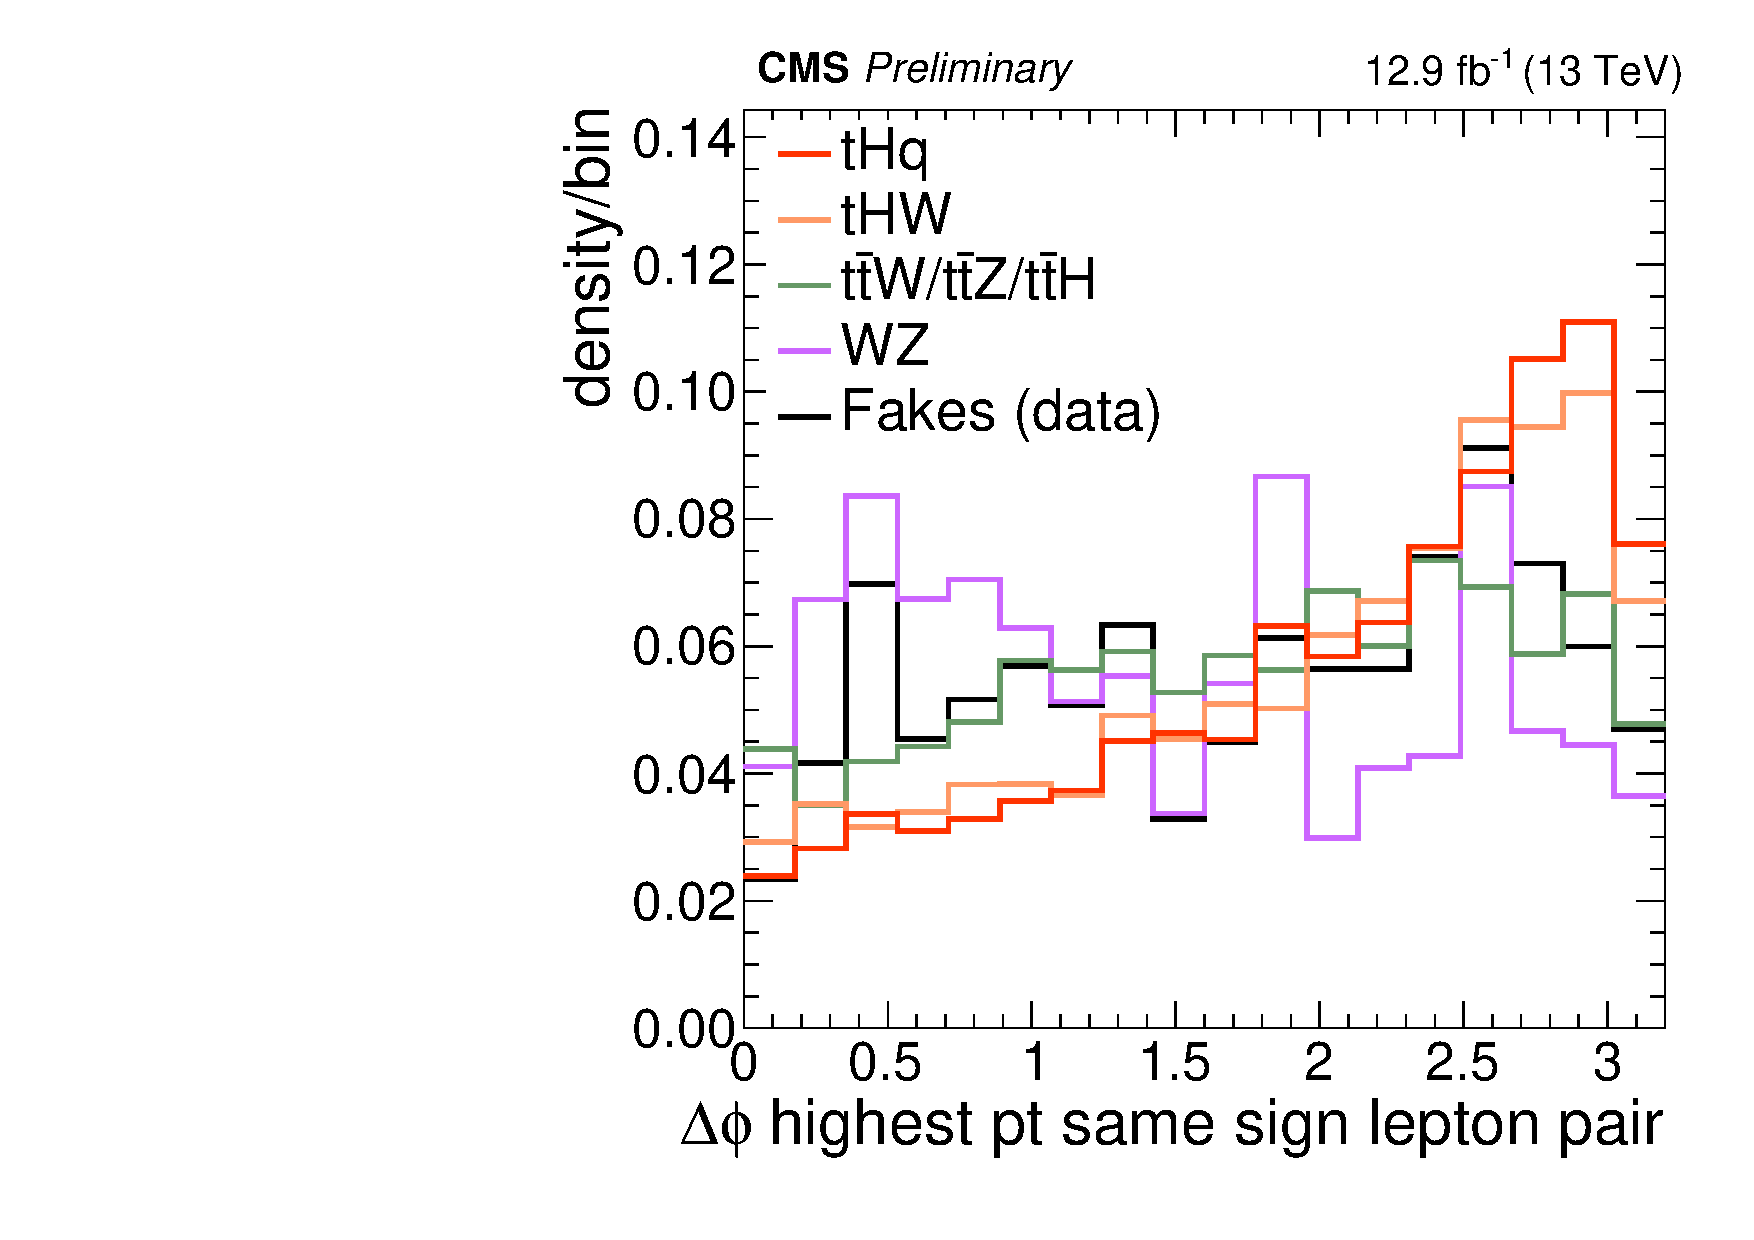
\includegraphics[width=0.245\textwidth]{figures/dPhiHighestPtSSPair.pdf}
 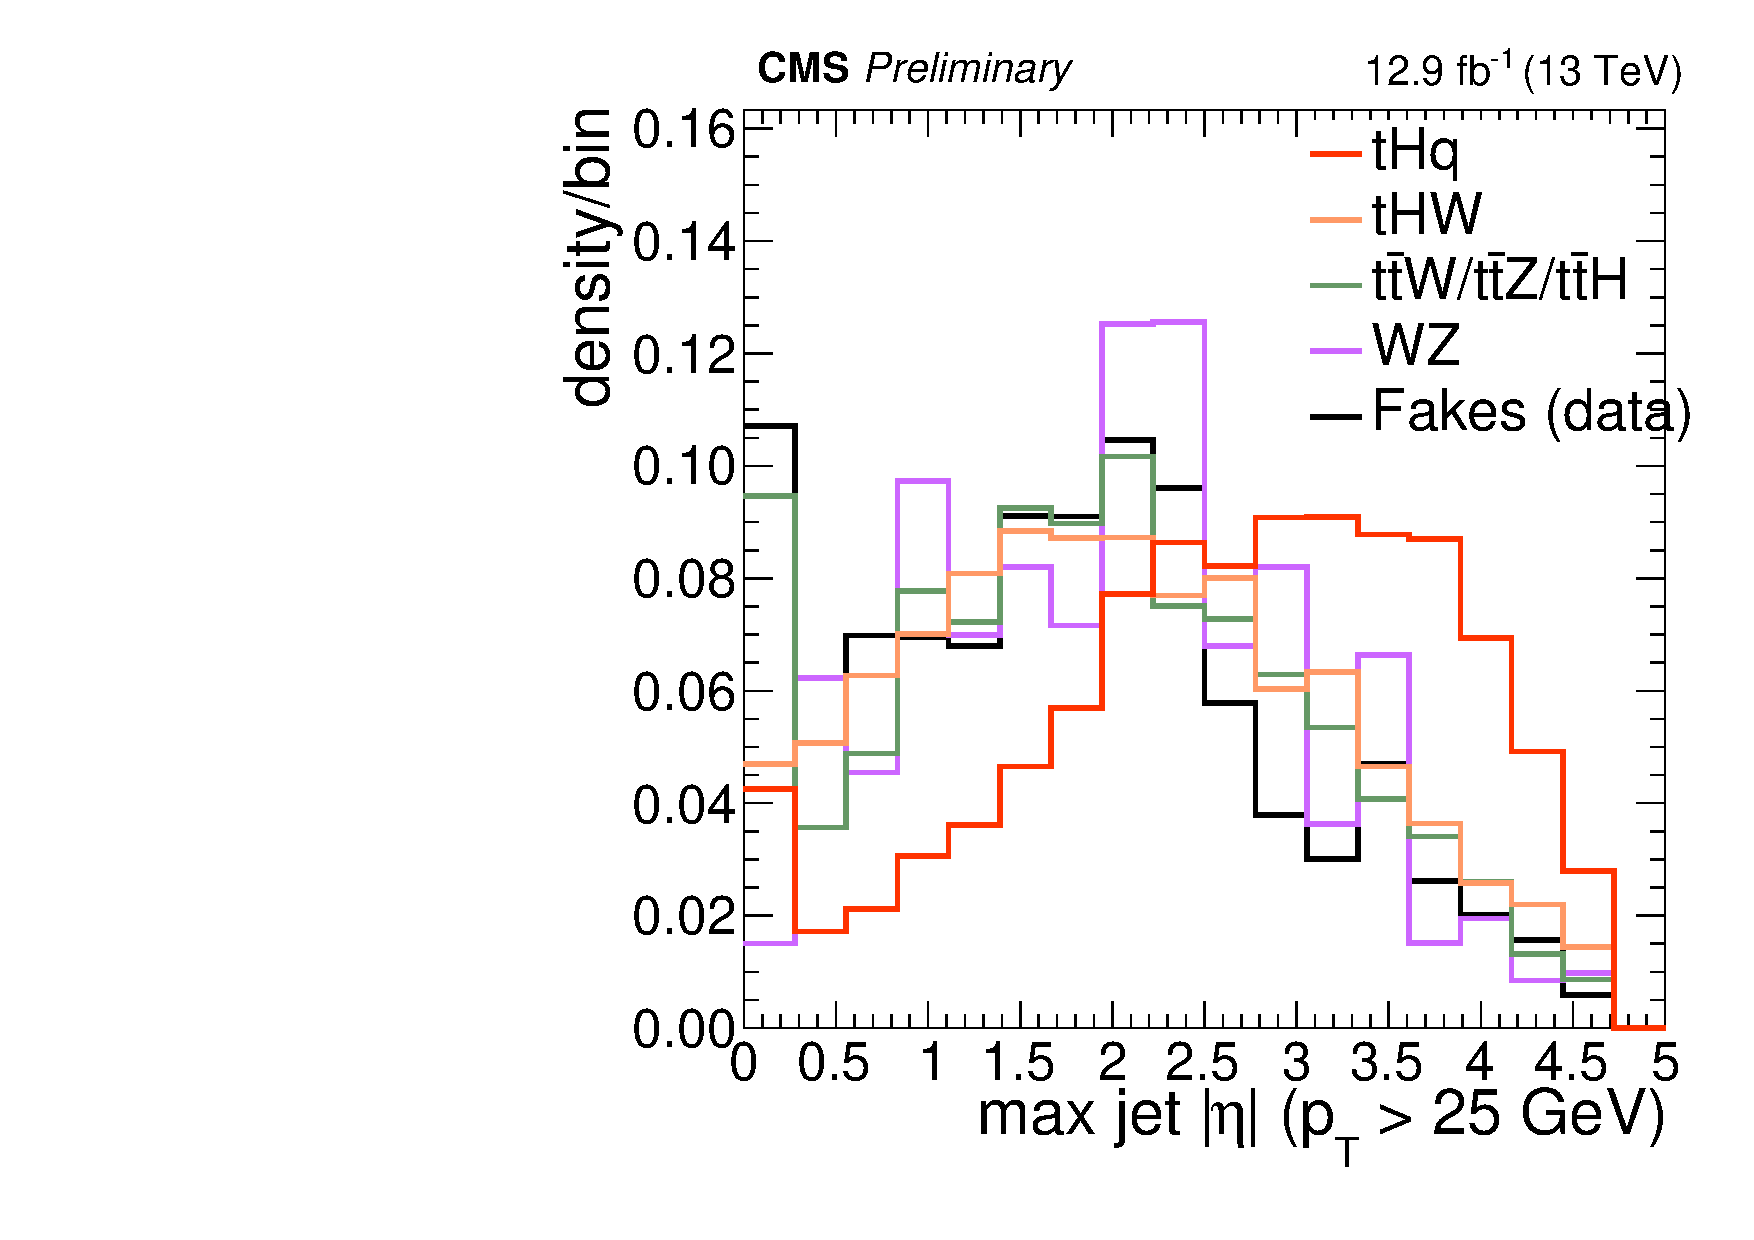
\includegraphics[width=0.245\textwidth]{figures/maxEtaJet25.pdf}
 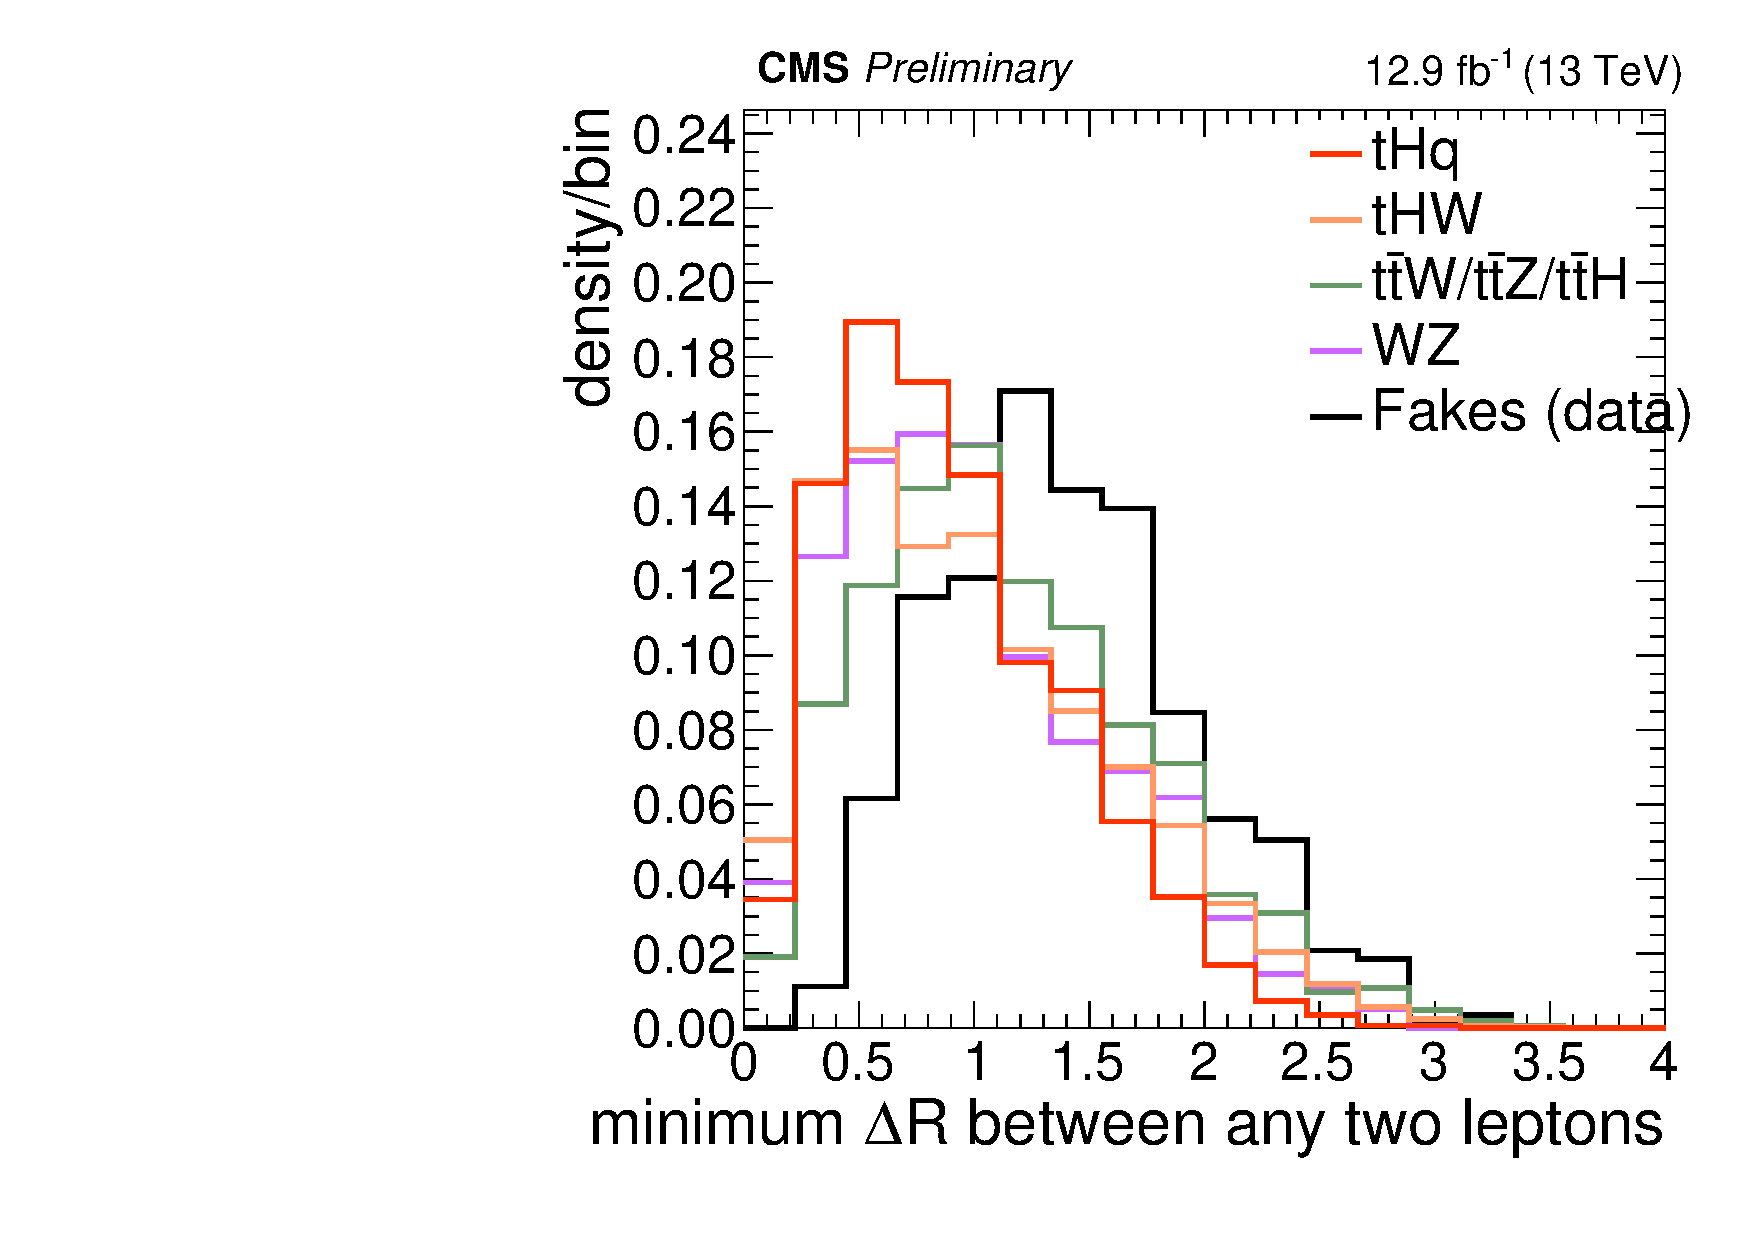
\includegraphics[width=0.245\textwidth]{figures/minDRll.pdf}
 \includegraphics[width=0.245\textwidth]{figures/nJet25.pdf} \\
 \includegraphics[width=0.245\textwidth]{figures/nJetEta1.pdf}
 \includegraphics[width=0.245\textwidth]{figures/totCharge.pdf}
\caption{Distributions of input variables to the BDT for signal discrimination, three lepton channel.} 
\label{fig:input_vars_3l}
\end{figure}    

\begin{figure} [!h]
  \centering
  \includegraphics[width=0.245\textwidth]{figures/Lep2Pt_mumu.pdf} 
  \includegraphics[width=0.245\textwidth]{figures/dEtaFwdJetBJet_mumu.pdf}
  \includegraphics[width=0.245\textwidth]{figures/dEtaFwdJet2BJet_mumu.pdf}
  \includegraphics[width=0.245\textwidth]{figures/dEtaFwdJetClosestLep_mumu.pdf} \\
  \includegraphics[width=0.245\textwidth]{figures/dPhiHighestPtSSPair_mumu.pdf}
  \includegraphics[width=0.245\textwidth]{figures/maxEtaJet25_mumu.pdf}
  \includegraphics[width=0.245\textwidth]{figures/minDRll_mumu.pdf}
  \includegraphics[width=0.245\textwidth]{figures/nJet25_mumu.pdf} \\
  \includegraphics[width=0.245\textwidth]{figures/nJetEta1_mumu.pdf}
  \includegraphics[width=0.245\textwidth]{figures/totCharge_mumu.pdf}
 \caption{Distributions of input variables to the BDT for signal discrimination, two lepton same sign channel.}
\label{fig:input_vars_2lss}
\end{figure}    

The MVA analysis consist of two stages: first a ``training'' where the MVA method is trained to discriminate between simulated signal and background events, then a ``test'' stage where the trained algorithm is used to classify different events from the samples.
The sample is obtained from a pre-selection (see Tab.~\ref{tab:evsel} with pre-selection cuts).

Figures~\ref{mva_input_tt} and~\ref{mva_input_ttv} show the input variables distributions as seen by the MVA algorithm.
Note that in contrast to the distributions in Fig.~\ref{fig:input_vars_3l} only the main backgrounds (\ttbar\ from simulation, \ttV) are included.

\begin{figure} [!h]
  \centering
  \includegraphics[width=\textwidth]{figures/mva_input1_tt.pdf}
  \includegraphics[width=\textwidth]{figures/mva_input2_tt.pdf}
\caption{BDT inputs as seen by TMVA (signal, in blue, is \tHq, background, in red, is \ttbar) for the three lepton channel, discriminated against \ttbar\ (fakes) background.} 
\label{mva_input_tt}
\end{figure}

\begin{figure} [!h]
  \centering
  \includegraphics[width=\textwidth]{figures/mva_input1_ttv.pdf}
  \includegraphics[width=\textwidth]{figures/mva_input2_ttv.pdf}
\caption{BDT inputs as seen by TMVA (signal, in blue, is \tHq, background, in red, is \ttW+\ttZ) for the three lepton channel, discriminated against \ttV\ background.}                                                                                                                                                         
\label{mva_input_ttv}
\end{figure}

The input variables distributions for 2lss channel for signal against the \ttbar\ and \ttV\ are shown in Figure~\ref{mva_input_2lss_tt} and Figure~\ref{mva_input_2lss_ttv} respectively.
\begin{figure} [!h]
  \centering
  \includegraphics[width=\textwidth]{figures/6var_tt.pdf}
  \includegraphics[width=0.66\textwidth]{figures/4var_tt.pdf}
\caption{BDT inputs as seen by TMVA (signal, in blue, is \tHq, background, in red, is \ttbar) for the same sign dilepton channel, discriminated against \ttbar\ background.} 
\label{mva_input_2lss_tt}
\end{figure}

\begin{figure} [!h]
  \centering
  \includegraphics[width=\textwidth]{figures/6var_ttv.pdf}
  \includegraphics[width=0.66\textwidth]{figures/4var_ttv.pdf}
\caption{BDT inputs as seen by TMVA (signal, in blue, is \tHq, background, in red, is \ttW+\ttZ) for the same sign dilepton channel, discriminated against \ttV\ background.}
\label{mva_input_2lss_ttv}
\end{figure}

Note that splitting the training in two groups reveals that some variables show opposite behavior for the two background sources; potentially screening the discrimination power if they were to be used in a single discriminant.
For some other variables the distributions are similar in both background cases.

From table~\ref{tab:bdtinputs}, it is clear that the input variables are correlated to some extend. These correlations play an important role for some MVA methods like the Fisher discriminant method in which the first step consist of performing a linear transformation to an phase space where the correlations between variables are removed. In case a boosted decision tree (BDT) method however, correlations do not affect the performance.

Figure~\ref{mva_corr} show the linear correlation coefficients for signal and background for the two training cases (the signal values are identical by construction). As expected, strong correlations appears for variables related to the forward jet activity. Same trend is seen in case of the same sign dilepton channel in Figure~\ref{mva_corr_2lss}.

\begin{figure} [!h]
  \centering
   \includegraphics[width=0.32\textwidth]{figures/corr_signal.pdf}
   \includegraphics[width=0.32\textwidth]{figures/corr_tt.pdf}
   \includegraphics[width=0.32\textwidth]{figures/corr_ttv.pdf}

\caption{ Signal (left), \ttbar\ background (middle), and \ttV\ background (right.) correlation matrices for the input variables in the TMVA analysis for the three lepton channel.}
\label{mva_corr}
\end{figure}

\begin{figure} [!h]
  \centering
  \includegraphics[width=0.32\textwidth]{figures/sig_corr_tt_2lss.pdf}
  \includegraphics[width=0.32\textwidth]{figures/bkg_corr_tt_2lss.pdf}
  \includegraphics[width=0.32\textwidth]{figures/bkg_corr_ttv_2lss.pdf}
\caption{Signal and Background correlation matrices for the input variables in the TMVA analysis for the same sign dilepton channel, for the signal (left), \ttbar\ background (middle), and \ttV\ background (right.)}
\label{mva_corr_2lss}
\end{figure}

\subsection{Classifiers response}
Several MVA algorithms were evaluated to determine the most appropriate method for this analysis.
The plots in Fig.~\ref{roc} (top) show the background rejection as a function of the signal efficiency for \ttbar\ and \ttV\ trainings (ROC curves) for the different algorithms that were evaluated.

\begin{figure} [!h]
  \centering
   \includegraphics[width=0.4\textwidth]{figures/roc_ttv_3l_multimva.pdf}
   \includegraphics[width=0.4\textwidth]{figures/roc_tt_3l_multimva.pdf} \\
   \includegraphics[width=0.4\textwidth]{figures/bdt_response_ttv_3l.pdf}
   \includegraphics[width=0.4\textwidth]{figures/bdt_response_tt_3l.pdf}
\caption{Top: background rejection vs signal efficiency (ROC curves) for various MVA classifiers (top) in the three lepton channel against \ttV\ (left) and \ttbar\ (right). Bottom: classifier output distributions for the gradient boosted decision trees, for training against \ttV\ (left) and against \ttbar\ (right).}
\label{roc}
\end{figure} 

\begin{figure} [!h]
  \centering
   \includegraphics[width=0.4\textwidth]{figures/roc_ttv_2lss.pdf}
   \includegraphics[width=0.4\textwidth]{figures/roc_tt_2lss.pdf} \\
   \includegraphics[width=0.4\textwidth]{figures/bdt_output_ttv_2lss.pdf}
   \includegraphics[width=0.4\textwidth]{figures/bdt_output_tt_2lss.pdf}
\caption{Top: background rejection vs signal efficiency (ROC curve) in the same sign dilepton channel for a single discriminator: BDTG, against \ttV\ (left) and \ttbar\ (right). Bottom: classifier output distribution, for training against \ttV\ (left) and against \ttbar\ (right).}
\label{output_2lss}
\end{figure}

In both cases the gradient boosted decision tree (``BDTA\_GRAD'') classifier offers the best results, followed by an adaptive BDT classifier (``BDTA''). 
The BDTA\_GRAD classifier output distributions for signal and backgrounds are shown on the bottom of Fig.~\ref{roc}.
As expected, a good discrimination power is obtained using default discriminator parameter values, with minimal overtraining.
TMVA provides a ranking of the input variables by their importance in the classification process, shown in Tab.~\ref{ranking}.

\begin{table}[h!]
\centering
\footnotesize
\begin{tabular}{lllll}
      &\multicolumn{2}{c}{ttbar training}             & \multicolumn{2}{c}{ttV training}\\\hline
Rank  & Variable             & Importance  & Variable             & Importance \\ \hline
    1 & minDRll              & 1.329e-01   & dEtaFwdJetBJet       & 1.264e-01\\
    2 & dEtaFwdJetClosestLep & 1.294e-01   & Lep3Pt               & 1.224e-01\\
    3 & dEtaFwdJetBJet       & 1.209e-01   & maxEtaJet25          & 1.221e-01\\
    4 & dPhiHighestPtSSPair  & 1.192e-01   & dEtaFwdJet2BJet      & 1.204e-01\\
    5 & Lep3Pt               & 1.158e-01   & dEtaFwdJetClosestLep & 1.177e-01\\
    6 & maxEtaJet25          & 1.121e-01   & minDRll              & 1.143e-01\\
    7 & dEtaFwdJet2BJet      & 9.363e-02   & dPhiHighestPtSSPair  & 9.777e-02\\
    8 & nJetEta1             & 6.730e-02   & nJet25\_Recl         & 9.034e-02\\
    9 & nJet25\_Recl         & 6.178e-02   & nJetEta1             & 4.749e-02\\
   10 & lepCharge            & 4.701e-02   & lepCharge            & 4.116e-02\\\hline

\end{tabular}
\caption{TMVA input variables ranking for BDTA\_GRAD method for the trainings in the three lepton channel. For both trainings the rankings show almost the same 5 variables in the first places.}

\label{ranking}
\end{table}

\begin{table}[h!]
\centering
\footnotesize
\begin{tabular}{lllll}
      &\multicolumn{2}{c}{ttbar training}             & \multicolumn{2}{c}{ttV training}\\\hline
Rank  & Variable             & Importance  & Variable             & Importance \\ \hline
    1 & dEtaFwdJetClosestLep & 1.394e-01   & maxEtaJet25          & 1.357e-01\\ 
    2 & minDRll              & 1.359e-01   & dEtaFwdJet2BJet      & 1.267e-01\\
    3 & maxEtaJet25          & 1.308e-01   & dEtaFwdJetBJet       & 1.200e-01\\
    4 & dPhiHighestPtSSPair  & 1.116e-01   & Lep2Pt               & 1.196e-01\\
    5 & Lep2Pt               & 1.111e-01   & dEtaFwdJetClosestLep & 1.145e-01\\
    6 & dEtaFwdJetBJet       & 1.067e-01   & minDRll              & 1.077e-01\\
    7 & dEtaFwdJet2BJet      & 8.906e-02   & nJet25\_Recl         & 1.020e-01\\
    8 & nJetEta1             & 6.445e-02   & dPhiHighestPtSSPair  & 8.232e-02\\
    9 & nJet25\_Recl         & 6.254e-02   & nJetEta1             & 5.948e-02\\
   10 & lepCharge            & 4.848e-02   & lepCharge            & 3.198e-02\\ \hline
\end{tabular}
\caption{TMVA input variables ranking for BDTA\_GRAD method in same-sign dilepton channel.}
\label{ranking}
\end{table}


The TMVA settings used in the BDT training are shown in Tab.~\ref{tab:bdtsettings}.

\begin{table}
\centering
\begin{tabular}{l}
  \hline
  \verb|TMVA.Types.kBDT| \\
  \verb|NTrees=800| \\
  \verb|BoostType=Grad| \\
  \verb|Shrinkage=0.10| \\
  \verb|!UseBaggedGrad| \\
  \verb|nCuts=50| \\
  \verb|MaxDepth=3| \\
  \verb|NegWeightTreatment=PairNegWeightsGlobal| \\
  \verb|CreateMVAPdfs| \\
  \hline
\end{tabular}
\caption{TMVA configuration used in the BDT training.}\label{tab:bdtsettings}
\end{table}


\section{Additional discriminating variables}

Two additional discriminating variables were tested considering the fact that the forward jet in the background could come from the pileup; since we have a real forward jet in the signal, it could give some improvement in the discriminating power. The additional variables describe the forward jet momentum (fwdJetPt25) and the forward jet identification(fwdJetPUID). Distributions for these variables in the three lepton channel are shown in the figure ~\ref{fwd_add_var_3l}. The forward jet identification distribution show that for both, signal and background, jets are mostly real jets. 

\begin{figure} [!h]
  \centering
   \includegraphics[width=0.9\textwidth]{figures/fwd_add_var_ttv_3l.pdf}\\
   \includegraphics[width=0.9\textwidth]{figures/fwd_add_var_tt_3l.pdf}
\caption{Additional discriminating variables distributions for ttv training(Top row) and tt training (bottom row) in the three lepton channel. The origin of the jets in the forward jet identification distribution is tagged as 0 for ``pileup jets'' while ``real jets'' are tagged as 1.}
\label{fwd_add_var_3l}
\end{figure}

The testing was made including in the MVA input one variable at a time, so we can evaluate the dicrimination power of each variable, and then both simultaneously. fwdJetPUID was ranked in the last place in importance (11) in both training (ttV and tt) while fwdJetPt25 was ranked 3 in the ttV training and 7 in the tt training. When training using 12 variables, fwdJetPt25 was ranked 5 and 7 in the ttV and tt trainings respectively, while fwdJetPUID was ranked 12 in both cases.

The improvement in the discrimination performance provided by the additional variables is about 1\%, so we decided not to include them in the current procedure. Table ~\ref{tab:add_var_improvement} show the ROC-integral for all the testing cases we made.


\begin{table}
\centering
\begin{tabular}{lc}
  \hline
                 &  ROC-integral \\\hline               
base 10 var ttv  & 0.848\\
+ fwdJetPUID ttv & 0.849\\
+ fwdJetPt25 ttv & 0.856\\
12 var ttv       & 0.856\\\hline\hline
base 10 var tt   & 0.777\\
+ fwdJetPUID tt  & 0.777\\
+ fwdJetPt25 tt  & 0.787\\
12 var           & 0.787\\\hline

\end{tabular}
\caption{ROC-integral for all the testing cases we made in the evaluation of the additional variables discriminating power. The improvement in the discrimination performance provided by the additional variables is about 1\% }\label{tab:add_var_improvement}
\end{table}

\clearpage

\section{Signal extraction}
\label{sec:extraction}
Despite the event selection requirements previously described, the post-selection yields are still dominated by the backgrounds,
and have insufficient statistics to determine the presence of the ttH signal, making further discrimination necessary.
The approach adopted in this search is to split the selected events into several mutually exclusive categories with
different signal to background ratios.
In each of these categories the signal is extracted from the distribution of a suitable discriminating variable.

In order to exploit the topological characteristics and specificities of the ttH signal with respect to the most
dominant backgrounds, the output of the boosted decision tree (BDT), trained using a selection of kinematic
variables, is used as the discriminating variable for the signal extraction.
In this analysis, the samples used for BDT training and evaluation are the ones reported in Sec. \ref{sec:samples}.

Both final states with two same sign leptons (2lss) and at least three leptons ($\geq$=3l) have dominant backgrounds originating
from the \ttbar\ and \ttV\ (V=W/Z) processes. In order to have an efficient discrimination against both of these processes,
a two-dimensional (2D) BDT approach is introduced. For each of the 2lss and $\geq$=3l final states, the BDT is separately trained
against the \ttbar\ and \ttV, selecting a set of kinematic variables that provide the largest separation in each training. The BDT
outputs of the training against these two processes are used to construct the 2D space, effectively a scatter plot of the
two discriminators. The consequent 2D distribution is then partitioned to rectangular sectors and ttH signal and background contributions
of each sector are summed and folded to a one-dimensional histogram. With a
convenient partitioning of the 2D space, the resulting difference of the signal and background shapes is enhanced with respect to the
one-dimensional case, for example against the \ttbar, and that is provided by the training of the additional BDT, against the \ttV\  process.

In the following subsections we detail the definitions of the BDTs used as discriminating variable for the signal extraction
in the 2lss and $\geq$=3l categories. We then describe the criterion to decide the binning of the 2D BDT.
Finally, we detail the precise event subcategorization.

\subsection{2lss event BDT}\label{sec:2lss event BDT}
The training is performed using a relaxed event selection that requires at least two preselected same sign leptons with leading and trailing lepton transverse momentum larger than 25 and 15 GeV, respectively, plus at least four jets in the event of which either two loose selected b-jets or one medium b-tagged jet.

The training against the \ttbar background is performed considering the following input variables:
\begin{itemize}
\item maximum absolute pseudorapidity of the two leading leptons
\item multiplicity of hadronic jets
\item minimum distance between the leading lepton and closest jet
\item minimum distance of the trailing lepton and closest jet
%\item missing transverse energy
%\item average separation between the two jets and the transverse mass of the leading lepton 
\item transverse mass of the leading lepton and missing transverse energy
\item hadronic top reconstruction (score of the discriminator for best permutation)
\end{itemize}

The training against the \ttV\  background is performed considering the following input variables:
\begin{itemize}
\item maximum absolute pseudorapidity of the two leading leptons
\item multiplicity of hadronic jets
\item minimum distance between the leading lepton and closest jet
\item minimum distance of the trailing lepton and closest jet
\item transverse mass of the leading lepton and missing transverse energy
\item leading lepton transverse momentum 
\item trailing lepton transverse momentum
%\item HT, defined as the scalar sum of the pT of the selected leptons, jets, and the met
\item Hj tagger score after hadronic top jets triplet removal (best permutation)
%\item Hj and Hjj taggers after hadronic top jets triplet removal
\end{itemize}

%The variables listed above are the same used in the previous versions of the analyses,
%with the exception of HT, which is now used in the training against \ttV\, and the last-itemized for both trainings.
The sets of observables listed above include new variables that have not been used before, such as the 
score of the hadronic top reconstruction and the Hj tagger, which are explained in more detail below.
The aforementioned hadronic top jet triplet, when using the Hj tagger in the training against the \ttV\ background,
indicates a triplet of jets with the highest likelihood to orginate from hadronic top decay in 2lss events.
This jet triplet is found through the event reconstruction BDT explained below, whose score is used as an input in the training against \ttbar.
The Hj tagger, described more in detail in the following,
is an algorithms designed to identify jets originating from one of the W of the Higgs in 2lss events.
The Higgs jets search is performed against all the jets that enter the 2lss region, except those forming a triplet compatible
with an hadronic top decay (from which the expression hadronic top jets triplet removal).

\subsubsection{Hadronic top reconstruction}
The reconstruction of the hadronic top decay is performed with a BDT. The objective is to correctly match
each selected jet and lepton to a final state particle in a $t\bar{t}H$ event, then
use the BDT response and other variables from the reconstruction to discriminate
against events without a hadronic top.     

Event reconstruction targets the 2lss category, specifically where the Higgs decays
to $W$ bosons. In the 2lss category, this means that one lepton originates from the
top system, and the other from the Higgs. For the jets, one of the
$W$ bosons from the Higgs decays hadronically, one of the top quarks decays
hadronically, producing a total of two b-jets, and four light-flavor jets
from the hadronic $W$ decays.   

{\bfseries Training}

The event reconstruction BDT is trained using the $t\bar{t}H$ monte-carlo powheg
signal sample described previously. 

The signal is correctly matched $t\bar{t}H$ events, which pass the 2lss selection.
Because the 2lss event selection requires at least four jets, the vast majority of signal
events used for training are only partially reconstructed, since a full reconstruction
necessitates six matched jets. Because so few events can be fully reconstructed, we must
consider partial reconstructions for events that have fewer than six matched jets.
The strategy for this is to use 'null' jets whose four-vectors are set to zero to
substitute missing jets in the event. Finally we require the signal events to have two
correctly matched selected leptons, and at least four correctly matched selected jets.

The background consists of all jet and lepton permutations of incorrectly matched
$t\bar{t}$ events. For the background, the null jets are added according to the
jet multiiplicity. For events with seven or fewer selected jets, three null jets are
added, for events with eight selected jets, two null jets are added, and one null jet
is added for events with greater than eight selected jets. To reduce the computation
time and improve performance,
several cuts are applied at each permutation to remove unlikely reconstructions.
These cuts include applying the b-tag requirement on the two jets being considered
as b-jets (1 b-tight, 2 b-loose) described earlier, requiring that no
reconstructed $W$ have a mass greater than 120 GeV, requiring the leptonic top mass
be less than 180 GeV, and requiring 
the hadronic top mass be less than 220 GeV. Additionally, we ignore permutations
arising from swapping two light flavor jets from the same $W$ boson, as the reconstruction is
identical. 

The BDT uses eight input variables, consisting of the CSV of the b-jets from the top
system, the transverse
momentum of the reconstructed hadronic top, the mass of the reconstructed hadronic top,
the mass of the $W$ originating from the hadronic top, the transverse momentum ratio
of lepton from the Higgs with the lepton from the top, and the solid angles between
the lepton from the top and
each b-jet from the top system, and between the lepton from the Higgs.
This approach focuses on the hadronic top decay, as the other aspects of the event
are more difficult to reconstruct due to the missing energy from the neutrinos. 

{\bfseries Evaluation}

The event reconstruction BDT is evaluated by iterating over all possible lepton and jet
permutations, and selecting the highest scoring permutation as the reconstruction for
each event. For the evaluation and usage, the null jet prescription and permutation
cuts used are identical to the background training.
The reconstruction is designed identify events that have a hadronic top present and thus offers
some discrimination against the semi-leptonic $t\bar{t}$ background, shown below in
Figure~\ref{reconstruction:outputVars}.


\begin{figure}[htb]
 \centering
   \includegraphics[width=0.4\textwidth]{plots_reconstruction/had_top_mass.png}
   \includegraphics[width=0.4\textwidth]{plots_reconstruction/had_top_pt.png}\\
   \includegraphics[width=0.4\textwidth]{plots_reconstruction/bdt_score.png}
   \caption{Best BDT score and associated quantities from hadronic top reconstruction.}
  \label{reconstruction:outputVars}
\end{figure}

%% \begin{figure}[htb]
%%  \centering
%%    \includegraphics[width=0.7\textwidth]{plots_reconstruction/roc_improvement.png}
%%    \caption{ROC curve of signal extraction BDT with and without reconstruction variables evaluated against $t\bar{t}$.}
%%   \label{reconstruction:roc}
%% \end{figure}


%% \begin{figure}[htb]
%%  \centering
%%    \includegraphics[width=0.7\textwidth]{plots_reconstruction/reconstruction_mva_csv_signal_region.png}
%%    \includegraphics[width=0.7\textwidth]{plots_reconstruction/reconstruction_topmass_toppt_signal_region.png}
%%    \caption{Event reconstruction variables in the 2lss signal region.}
%%   \label{reconstruction:vars_signal_region}
%% \end{figure}

%% \begin{figure}[htb]
%%  \centering
%%    \includegraphics[width=0.7\textwidth]{plots_reconstruction/reconstruction_mva_csv_application_region.png}
%%    \includegraphics[width=0.7\textwidth]{plots_reconstruction/reconstruction_topmass_toppt_application_region.png}
%%    \caption{Event reconstruction variables in the 2lss application region.}
%%   \label{reconstruction:vars_application_region}
%% \end{figure}

%% \begin{figure}[htb]
%%  \centering
%%    \includegraphics[width=0.7\textwidth]{plots_reconstruction/reconstruction_extraction_mva_output.png}
%%    \caption{Signal extraction MVA output with and with out signal extraction.}
%%   \label{reconstruction:extraction_output}
%% \end{figure}

\clearpage
\subsubsection{The Hj tagger}\label{sec:Hjtagger}
In this section we describe a discriminator aiming at identifying jets that originates from a Higgs decaying to two Ws.
In particular, we target the 2lss category in which the ttH signal decays, in the highest fraction of events, according to the following chain:
$$(t) (t) (H) \rightarrow  (bW) (bW) (WW^*) \rightarrow (bjj)  (b\ell\nu_{\ell}) (\ell\nu_{\ell}jj)$$
We therefore expect 2 b quark jets, 4 jets, 2 same-sign leptons, and missing energy in the final state,
altough, in order to increase the signal acceptance, the analysis requires the presence of at least 4 jets overall.
This means that the Higgs jets do not necessarily enter the signal region.

In order to deal with both the complicated jet combinatoric and the possibility that not all the jets originating from Higgs are selected,
one discriminator is developed: the Higgs-jet (Hj) tagger.
The Hj tagger is an object discriminator that exploits jet identification and kinematic properties
in order to assess the likelihood of a jet of originating in the decay $H \rightarrow WW^* \rightarrow \ell\nu_{\ell}jj$.

The discriminator is developed considering the BDT  multivariate technique.
We rely on the powheg ttH sample and ttV sample to define the signal and the background in the training.
For the Hj tagger the signal is represented by reconstructed jets that are matched at gen-level to jets
of the process $H \rightarrow WW^* \rightarrow \ell\nu_{\ell}jj$, while the background is given by the reconstructed jets in ttV events. 
For the training, we consider the phase space of events that enter the 2lss category, with 0 $\tau_h$.

In the following subsection we list the variables used for the Hj taggers and their expected BDT distributions.

{\bfseries Hj variables and performances}\\
The variables used for the Hj tagger are:
\begin{itemize}
\item minimum dR of the jet and one of the lepton
\item maximum dR of the jet and one of the lepton
\item jet pT
\item jet b-tagging discriminator
\item jet quark-gluon discriminator
\end{itemize}

The performances of the Hj tagger are illustrated in Fig. \ref{fig:HjDistrROC}.
The ROC curve (Fig. \ref{fig:HjDistrROC}, right) highlights the improvement
in performance of the Moriond 2017 BDT (red line) versus the ICHEP 2016 BDT (black line).

\begin{figure}[htb]
 \centering
   \includegraphics[width=0.48\textwidth]{plots_HjHjj/Jtagger_Ks_.png}
   \includegraphics[width=0.48\textwidth]{plots_HjHjj/Roc_Comparison_18Feb.pdf}
   \caption{The Hj distribution (left) and ROC (right). The ROC curve highlights the improvement in performance of the Moriond 2017 BDT (red line) versus            the ICHEP 2016 BDT (black line). Signal and background composition are described in the text.}
   %\caption{The Hj ROC. Signal and background composition are described in the text.}
  \label{fig:HjDistrROC}
\end{figure}

Figures~\ref{fig:2lss_training_1} and \ref{fig:2lss_training_2} show a comparison of the simulated signal (ttH) and background (\ttbar\ or \ttV) processes for each of the input variables to the BDT discriminator.
Figure ~\ref{fig:2l_mvaTraining} shows the separation power of the BDT discriminators.
%while Figures~\ref{fig:2l_mvaOutput} shows the distributions of these discriminators.

\begin{figure}[htb]
        \centering
\includegraphics[width=0.32\textwidth]{plots_extraction/training/2lss/kinMVA_input_max_Lep_eta.pdf}
\includegraphics[width=0.32\textwidth]{plots_extraction/training/2lss/kinMVA_input_numJets.pdf}\\
\includegraphics[width=0.32\textwidth]{plots_extraction/training/2lss/kinMVA_input_mindr_lep1_jet.pdf}
\includegraphics[width=0.32\textwidth]{plots_extraction/training/2lss/kinMVA_input_mindr_lep2_jet.pdf}
%\includegraphics[width=0.32\textwidth]{plots_extraction/training/2lss/kinMVA_input_met.pdf}
%\includegraphics[width=0.32\textwidth]{plots_extraction/training/2lss/kinMVA_input_avg_dr_jet.pdf}
        \caption{The separation power of the variables used for BDT trainings, in the two same sign leptons channel.}
        \label{fig:2lss_training_1}
\end{figure}

\begin{figure}[htb]
        \centering
\includegraphics[width=0.32\textwidth]{plots_extraction/training/2lss/kinMVA_input_MT_met_lep1.pdf}
\includegraphics[width=0.32\textwidth]{plots_extraction/training/2lss/kinMVA_input_LepGood0_conePt.pdf}\\
\includegraphics[width=0.32\textwidth]{plots_extraction/training/2lss/kinMVA_input_LepGood1_conePt.pdf}
\includegraphics[width=0.32\textwidth]{plots_extraction/training/2lss/kinMVA_input_BDTv8_eventReco_Hj_score.pdf}
%\includegraphics[width=0.32\textwidth]{plots_extraction/training/2lss/kinMVA_input_BDTv8_eventReco_Hjj_score.pdf}
        \caption{The separation power of the variables used for BDT trainings, in the two same sign leptons channel.}
        \label{fig:2lss_training_2}
\end{figure}

\begin{figure}[htb]
%\captionsetup[subfigure]{labelformat=empty}
	\centering
%\begin{subfigure}
	%\centering
\includegraphics[width=0.35\textwidth]{plots_extraction/training/2lss/kinMVA_2lss_ttbar_withBDTv8.pdf}%kinMVA_2lss_ttbar.pdf}
\includegraphics[width=0.35\textwidth]{plots_extraction/training/2lss/kinMVA_2lss_ttV_withHj.pdf}%kinMVA_2lss_ttV.pdf}
	\caption{The separation power of the BDT output against the ttbar (left) and ttV (right) background, in the two same sign leptons channel.}
	\label{fig:2l_mvaTraining}
\end{figure}
%\end{subfigure}
%\bigskip
%\bigskip

%\begin{figure}[htb]
%	\centering
%%\includegraphics[width=0.35\textwidth]{plots_extraction/selection/2lss_SR/kinMVA_2lss_ttbar}
%%\includegraphics[width=0.35\textwidth]{plots_extraction/selection/2lss_SR/kinMVA_2lss_ttV}\\
%\includegraphics[width=0.35\textwidth]{plots_extraction/selection_data/2lss_SR/kinMVA_2lss_ttbar_withBDTv8.pdf}
%\includegraphics[width=0.35\textwidth]{plots_extraction/selection_data/2lss_SR/kinMVA_2lss_ttV_withHj.pdf}
%	\caption{Distribution of the discriminator against the ttbar (left) and ttV (right) backgrounds, in the two same sign leptons channel, with reducible background prediction from MC (top) and from data (bottom).}
%	\label{fig:2l_mvaOutput}
%\end{figure}

\clearpage
\subsection{3l event BDT}\label{sec:3lss event BDT}
The three lepton category has the following variables for the training against the \ttbar\ background:
\begin{itemize}
\item maximum absolute pseudorapidity of the two leading leptons
\item multiplicity of hadronic jets
\item minimum distance between the leading lepton and closest jet
\item minimum distance of the trailing lepton and closest jet.
\item transverse mass of the leading lepton and missing transverse energy
%\item missing HT
%\item average distance of the two jets
\end{itemize}

For the training against the \ttV\ background, the input variables are:
\begin{itemize}
\item maximum absolute pseudorapidity of the two leading leptons
\item transverse mass of the leading lepton and missing transverse energy
\item multiplicity of hadronic jets
\item minimum distance between the leading lepton and closest jet
\item minimum distance of the trailing lepton and closest jet
\item leading lepton transverse momentum and the third lepton transverse momentum.
\end{itemize}

Furthermore, the performance of the Matrix Element Method (MEM, as described in Appendix.~\ref{sec:mem}, on page~\pageref{sec:mem}) in the three lepton category warrants its inclusion as input to the training against the \ttV\ process. For ICHEP2016, the MEM was included using the log of weights for the \ttH, \ttW\ and \ttZ\ hypotheses.
For this iteration of the analysis, it was found that given the \ttV\ BDT parameters used, it is more efficient to include solely the likelihood of background vs signal + backgrounds (one variable instead of three). This improves the performance by a few percent.

In addition, it was found that the \ttbar\ BDT could also be improved by including the MEM among the input variables, using the MEM weights of \ttH, \ttbar, and the weights obtained from kinematic reconstruction of fully and semi leptonic ttH hypothesis are included. It improves the performance of the \ttbar\ BDT by about 5\%. \textit{In the current version of the analysis, this is not yet implemented because of CPU time constraints (MEM not yet run on the \ttbar\ sample).}

Because the currently available Monte-Carlo statistics prevent us from training with the full event selection, a relaxed selection has been
applied instead for training. This relaxed selection requires at least three preselected leptons where neither lepton pair has an invariant mass within
10 GeV of the mass of the Z boson, the leading, trailing and sub-trailing lepton transverse momentum larger than 25, 15 and 15 GeV,
respectively, the MET LD requirement applied and at least two loose selected b-jets in the event.
In Figures~\ref{fig:3l_training_1} and~\ref{fig:3l_training_2} a comparison of the simulated signal (ttH) and background (\ttbar\ or \ttV) processes for each of the input variables
to the BDT discriminator is presented. Further details on the BDT training are available in Appendix~\ref{app:BDTtraining}.

\begin{figure}[htb]
        \centering
\includegraphics[width=0.32\textwidth]{plots_extraction/training/3l/kinMVA_input_max_Lep_eta.pdf}
\includegraphics[width=0.32\textwidth]{plots_extraction/training/3l/kinMVA_input_MT_met_lep1.pdf}\\
\includegraphics[width=0.32\textwidth]{plots_extraction/training/3l/kinMVA_input_numJets.pdf}
%\includegraphics[width=0.32\textwidth]{plots_extraction/training/3l/kinMVA_input_mhtJet25.pdf}
%\includegraphics[width=0.32\textwidth]{plots_extraction/training/3l/kinMVA_input_avg_dr_jet.pdf}
\includegraphics[width=0.32\textwidth]{plots_extraction/training/3l/kinMVA_input_mindr_lep1_jet.pdf}
        \caption{The separation power of the variables used for BDT trainings, in the three lepton channel.}
        \label{fig:3l_training_1}
\end{figure}

\begin{figure}[htb]
        \centering
\includegraphics[width=0.32\textwidth]{plots_extraction/training/3l/kinMVA_input_mindr_lep2_jet.pdf}
\includegraphics[width=0.32\textwidth]{plots_extraction/training/3l/kinMVA_input_LepGood0_conePt.pdf}
\includegraphics[width=0.32\textwidth]{plots_extraction/training/3l/kinMVA_input_LepGood2_conePt.pdf}\\
\includegraphics[width=0.32\textwidth]{plots_extraction/training/3l/kinMVA_input_MEM_LR.pdf}
%\includegraphics[width=0.32\textwidth]{plots_extraction/training/3l/kinMVA_input_MEM_TTHfl.pdf}
%\includegraphics[width=0.32\textwidth]{plots_extraction/training/3l/kinMVA_input_MEM_TTW.pdf}
%\includegraphics[width=0.32\textwidth]{plots_extraction/training/3l/kinMVA_input_MEM_TTLL.pdf}
        \caption{The separation power of the variables used for BDT trainings, in the three lepton channel.}
        \label{fig:3l_training_2}
\end{figure}

Figure \ref{fig:3l_mvaOutput} shows the separation power of the BDT discriminators.
%while \ref{fig:3l_mvaOutput} shows the distributions of these discriminators.

%\begin{figure}[htb]
%        \centering
%%\begin{subfigure}
%	%\centering
%\includegraphics[width=0.35\textwidth]{plots_extraction/training/3l/kinMVA_3l_ttbar.pdf}
%\includegraphics[width=0.35\textwidth]{plots_extraction/training/3l/kinMVA_3l_ttV_withMEM.pdf}
%	\caption{The separation power of the BDT output against the ttbar (left) and ttV (right) background, in the three lepton channel.}
%	\label{fig:3l_mvaTraining}
%%\end{subfigure}
%\end{figure}

\begin{figure}[htb]
        \centering
	%\centering
%\includegraphics[width=0.35\textwidth]{plots_extraction/selection/3l_SR/kinMVA_3l_ttbar}
%\includegraphics[width=0.35\textwidth]{plots_extraction/selection/3l_SR/kinMVA_3l_ttV_withMEM}\\
\includegraphics[width=0.35\textwidth]{plots_extraction/selection_data/3l_SR/kinMVA_3l_ttbar.pdf}
\includegraphics[width=0.35\textwidth]{plots_extraction/selection_data/3l_SR/kinMVA_3l_ttV.pdf}
\caption{Distribution of the discriminator against the ttbar (left) and ttV (right) backgrounds, in the three lepton channel, with reducible background prediction from MC (top) and from data (bottom).}
\label{fig:3l_mvaOutput}
\end{figure}

\clearpage
\subsection{2D BDT binning}\label{sec:2lss event BDT}
The two-dimensional plane spanned by the ouptut of the two BDTs is populated by signal and background events in a non-uniform way: the two-dimensional distribution of the discriminators for the ttH signal (top), and for the ttbar (bottom left) and ttV (bottom right) backgrounds, are shown in Figures~\ref{fig:2l_2dmaps} and~\ref{fig:3l_2dmaps} for the same-sign dileptonic and the multileptonic inclusive signal regions, respectively. 

\begin{figure}[htb]
	\centering
        \includegraphics[width=0.35\textwidth]{plots_extraction/binning/2dmaps/tth_2l_2D}\\
        \includegraphics[width=0.35\textwidth]{plots_extraction/binning/2dmaps/tt_2l_2D}
        \includegraphics[width=0.35\textwidth]{plots_extraction/binning/2dmaps/ttw_2l_2D}
        \caption{Two-dimensional distribution of the discriminators for the \ttH signal (top), and for the \ttbar (bottom left) and \ttV\ (bottom right) backgrounds, in the two same sign leptons channel, estimated from MC.}
	\label{fig:2l_2dmaps}
\end{figure}

\begin{figure}[htb]
	\centering
        \includegraphics[width=0.35\textwidth]{plots_extraction/binning/2dmaps/tth_3l_2D}\\
        \includegraphics[width=0.35\textwidth]{plots_extraction/binning/2dmaps/tt_3l_2D}
        \includegraphics[width=0.35\textwidth]{plots_extraction/binning/2dmaps/ttw_3l_2D}
        \caption{Two-dimensional distribution of the discriminators for the \ttH~signal (top), and for the \ttbar~(bottom left) and \ttV~(bottom right) backgrounds, in the three lepton channel, estimated from MC.}
	\label{fig:3l_2dmaps}
\end{figure}

\begin{figure}[htb]
	\centering
        \includegraphics[width=0.35\textwidth]{plots_extraction/binning/3l/cookItUp}\\
        \caption{The discriminator of the $\mathrm{BDT(ttH,ttV)}$~classifier for simulated \ttV events, when the training is performed with or without the MEM discriminator among the input variables. A $\chi^{2}$ fit is performed, assuming linear dependence.}
	\label{fig:3l:cookItUp}
\end{figure}

The two-dimensional plane is then partitioned in several regions, depending on their different
signal or background composition, with the objective of maximizing the analysis sensitivity with the available luminosity. To do so, a method based on the likelihood ratio of signal and bakground is used.

Formally, this corresponds to building a multivariate classifier to reduce the dimensionality of the problem from two to one.

The plane is populated with events taken from simulated samples that are not used in the main analysis. Furthermore, for each simulated sample (\ttH signal, \ttbar and \ttV\ backgrounds) half of the events are used for training, and the other half are used to evaluate the performance of the classifier.

\textit{As the MEM method is vastly computer intensive, it has not been possible to compute the matrix element for the \ttbar~sample in the three leptons final state. For this reason, \ttV~events are used to assess the eventual correlation between the $\mathrm{BDT(ttH,ttV)}$ outputs obtained when training with or without the MEM discriminator among the inputs. Figure~\ref{fig:3l:cookItUp} shows the positive correlation found between the $\mathrm{BDT(ttH,ttV)}$ output in \ttV~events. A linear dependence is assumed, and under this assumption a function relating the non-MEM-trained BDT output and the MEM-trained BDT output is found via a $\chi^{2}$~fit to the \ttV~simulated events. The parameters of the fit are determined with 2--10\% accuracy, and the resulting estimator, $\hat{BDT}_{mem}(ttH,ttV) = 0.04804 + 0.6902\times BDT(ttH,ttV)_{nomem} $, is used in place of the output of the $\mathrm{BDT(ttH,ttV)}$ trained without MEM discriminator as an input. This relies on the assumption that the introduction of the MEM discriminator as an input to the $\mathrm{BDT(ttH,ttV)}$ training has the same effect in \ttbar~events as in \ttV~events. As soon as it will be possible to compute MEM for \ttbar~events, the conversion function will be removed.}

The plane, populated with training events, is binned finely, depending on the available statistics: the binning is finer ($20\times20$) for the two same sign leptons final state, and coarser ($10\times10$) for the three leptons final state. For each bin, the likelihood ratio between signal and background is computed.

In order to obtain an optimal one-dimensional classifier starting from the two-dimensional likelihood ratio distribution, an ordering criterion for the bins is devised. First the likelihood distribution for background events is obtained by assigning to each background event the likelihood ratio corresponding to the bin the event belongs to. The fine granularity of the binning ensures that this assignment is a good approximation of the true underlying likelihood function. From the distribution of the likelihood ratio for background events, the corresponding cumulative distribution is computed. A choice for the final number of bins is performed, by taking into account the available statistics in the training samples, and the quantiles of the cumulative likelihood ratio distribution for background distribution are used to divide it into the target number of final bins. The cumulative likelihood ratio distribution for background events, and its partition in quantiles, are shown in Fig.~\ref{fig:cumulative} for the two same sign leptons (left) and three leptons (right) final states respectively.

%The cumulative likelihood ratio distribution for background events, and its partition in quantiles, are shown in the left part of Fig.~\ref{fig:2l_likelihoodBinning}~and~\ref{fig:3l_likelihoodbinning}~for the two same sign leptons and three leptons (right) final states respectively.

The map between the initial and the final binning is shown in the left part of Fig.~\ref{fig:2l_likelihoodBinning}~and~\ref{fig:3l_likelihoodBinning}~for the two same sign leptons and three leptons final states respectively. Such construction guarantees that the final bins are populated by background events in an uniform way. The resulting one-dimensional distributions, obtained using the testing events, are shown in the right part of Fig.~\ref{fig:2l_likelihoodBinning}~and~\ref{fig:3l_likelihoodBinning}~for the two same sign leptons and three leptons final states respectively. The population of the background the testing distribution is not perfectly uniform in the testing sample because of statistical fluctuation of the testing and training samples. 

\begin{figure}[htb]
	\centering
        \includegraphics[width=0.35\textwidth]{plots_extraction/binning/2lss/cumulative_2lss}       
        \includegraphics[width=0.35\textwidth]{plots_extraction/binning/3l/cumulative_3l}\\
        \caption{Cumulative likelihood ratio distribution for background events for the two same sign leptons final state (left) and the three leptons final state (right), estimated from MC.}
	\label{fig:cumulative}
\end{figure}

\begin{figure}[htb]
	\centering
        \includegraphics[width=0.35\textwidth]{plots_extraction/binning/2lss/likelihoodBased_2d_2lss.png}
        \includegraphics[width=0.35\textwidth,height=0.35\textwidth]{plots_extraction/binning/2lss/likelihoodBased_1d_2lss}
        \caption{The location of the different bins in the two-dimensional plane (left), as well as the number of expected events in each bin (right) in the two same sign leptons channel, estimated from MC.}
	\label{fig:2l_likelihoodBinning}
\end{figure}


\begin{figure}[htb]
	\centering
        \includegraphics[width=0.35\textwidth]{plots_extraction/binning/3l/likelihoodBased_2d_3l.png}
        \includegraphics[width=0.35\textwidth,height=0.35\textwidth]{plots_extraction/binning/3l/likelihoodBased_1d_3l}
        \caption{The location of the different bins in the two-dimensional plane (left), as well as the number of expected events in each bin (right) in the three leptons channel, estimated from MC.}
	\label{fig:3l_likelihoodBinning}
\end{figure}

To check that the choice number of final bins in each final state is indeed suitable, an alternative method that does not require any assumption on the final number of bins is used, based on the $k$-means algorithm~\cite{MR0090073,macqueen1967} is used, yielding similar results and thus confirming the soundness of the choice of number of final bins. Such method is detailed in Appendix~\ref{sec:kmeans}.% {\it The number of bins is slightly higher in each final state because of the higher statistics samples used for this latest run. In a couple days we will provide updated plots for the appendix, using the same samples used for the likelihood ratio based method.}

%% \begin{table}[thb]
%% \centering
%% \caption{Coordinates of the bins that represent the partitioning of the 2D BDT plane.}
%% \label{tab:binning}
%% \begin{tabular}{lllllllllllllllll}
%% \hline
%%                    & bin 1 & bin 2 & bin 3 & bin 4 & bin 5 & bin 6 & bin 7\\
%% \hline
%% $2lss (\ttbar)$     & (-1.0, -0.2] & (-0.2, 0.1] & (0.1, 0.4] & (0.1, 0.4] & (0.4, 1.0] & (0.4, 1.0] & (0.4, 1.0] \\
%% $2lss (\ttV)$       & (-1.0, 1.0] & (-1.0, 1.0] & (-1.0, 0.3] & (0.3, 1.0] & (-1.0, 0.1] & (0.1, 0.4] & (0.4, 1.0]\\ \hline

%% $3\ell (\ttbar)$      & (-1.0, -0.3] & (-0.3, 0.3] & (-0.3, 0.3] & (0.3, 1.0]  & (0.3, 1.0]  & & \\
%% $3\ell (\ttV)$        & (-1.0, 1.0] & (-1.0, 0.25] & (0.25, 1.0] & (-1.0, 0.25] & (0.25, 1.0] & & \\

%% \hline
%% \end{tabular}
%% \end{table}

Figure~\ref{fig:kinMVA_binning} shows the event yield as a function of the bins defined above.

\begin{figure}[htb]
	\centering
\includegraphics[width=0.35\textwidth]{plots_extraction/selection_data/2lss_SR/kinMVA_2lss_bins8_withBDTv8_withHj_ourBinning.pdf}
\includegraphics[width=0.35\textwidth]{plots_extraction/selection_data/3l_SR/kinMVA_3l_bins5_ourBinning.pdf}
	\caption{Binned distributions of the pair of discriminators in 2lss (left) and 3l (right) channels.}
	\label{fig:kinMVA_binning}
\end{figure}

%\begin{figure}[htb]
%	\centering
%\includegraphics[width=0.35\textwidth]{plots_extraction/selection_data/2lss_SR/postfit_kinMVA_2lss_bins}
%\includegraphics[width=0.35\textwidth]{plots_extraction/selection_data/3l_SR/postfit_kinMVA_3l_bins}
%	\caption{\textbf{Post-fit} binned distributions of the pair of discriminators in 2lss (left) and 3l (right) channels.}
%	\label{fig:kinMVA_binning_postfit}
%\end{figure}


%\begin{figure}[htb]
%	\centering
%\includegraphics[width=0.4\textwidth]{plots_extraction/selection_data/2lss_SR/kinMVA_2lss_catbinIndex}
%\includegraphics[width=0.4\textwidth]{plots_extraction/selection_data/3l_SR/kinMVA_3l_catbinIndex}
%	\caption{Splitting in categories and BDT bins for the 2lss and 3l channels.}
%	\label{fig:catbinsplitting}
%\end{figure}

%% Don't forget to also reference it in the text
%% add when MEM weights available\begin{figure}[htb]
%% add when MEM weights available	\centering
%% add when MEM weights available\includegraphics[width=0.32\textwidth]{plots_extraction/selection_data/3l_SR/kinMVA_input_MEM_TTH}
%% add when MEM weights available\includegraphics[width=0.32\textwidth]{plots_extraction/selection_data/3l_SR/kinMVA_input_MEM_TTW}
%% add when MEM weights available\includegraphics[width=0.32\textwidth]{plots_extraction/selection_data/3l_SR/kinMVA_input_MEM_TTZ}
%% add when MEM weights available	\caption{MEM weights for ttH, ttW and ttZ hypotheses in the 3l channel.}
%% add when MEM weights available	\label{fig:memweights}
%% add when MEM weights available\end{figure}

\subsection{Event subcategories}

Events are further split into lepton flavours: two electrons, two muons and electron and muon. These three categories, except
the two electrons, are further divided according to the presence (or absence) of two medium tagged b-jets, the b-tight (b-loose) categories.

The events with at least three leptons are only separated into the b-tight and b-loose categories.

Finally, to exploit the charge asymmetry present in several backgrounds (ttW, WZ, single top and W+jets), but not present in ttH,
events in each of the categories described above are further categorized by the positive or negative sum of the lepton charges. The
summary of all event categories is summarized in Figure~\ref{fig:category_table}.

\begin{figure}[htb]
	\centering
\includegraphics[width=0.70\textwidth]{plots_extraction/categories/categories_notau.png}
	\caption{Diagram of all event categories in the analysis. Categories are based on lepton multiplicity and flavor,
         b-jet composition, and the sign of the sum of the lepton charges.}
	\label{fig:category_table}
\end{figure}

\begin{figure}[htb]
	\centering
\includegraphics[width=0.4\textwidth]{plots_extraction/selection_data/2lss_SR/2lep_catIndex.pdf}
\includegraphics[width=0.4\textwidth]{plots_extraction/selection_data/3l_SR/3lep_catIndex.pdf}
	\caption{Splitting in categories for the 2lss (left) and 3l (right) channels.}
	\label{fig:catsplitting}
\end{figure}




%\begin{figure}[htb]
%	\centering
%\includegraphics[width=0.4\textwidth]{plots_extraction/categories/kinMVA_2lss_bins7}
%\includegraphics[width=0.4\textwidth]{plots_extraction/categories/kinMVA_3l_bins5_withMEM}
%	\caption{Decay composition of the ttH signal in 2lss (left) and 3l (right) channels.
%\textit{We specify that all the plots related to MEM are still the ones produced during the ICHEP compaing and the MEM is currently not included in the results, altough we are currently reprocessing the MEM technique with the full 2016 data and plan to include it in the analysis.}
%}
%	\label{fig:splitting}
%\end{figure}
%

\subsection{Binning and selection optimization}\label{sec:binopt}
\emph{Note that the numbers in this subsection are upper limits on the \tHq+\tHW\ cross sections only (without \ttH), and are always evaluated at $\Ct=-1.0$, $\CV=1.0$.}
\hrule

The effect on the cross section limit of the choice of pre-selection cuts is evaluated by varying the most important cuts and re-calculating the limit (in the three lepton channel) in each case.
Table~\ref{cut_limit} shows the several variations made, compared to a baseline corresponding to the selection reported in Tab.~\ref{tab:evsel}, but with only a loose CSV jet and a \Z\ veto of $\pm10\GeV$.
The optimal limit is found when requiring a slightly tighter selection with respect to the baseline.
This is the selection reported in Tab.~\ref{tab:evsel}.

\begin{table}[h!]
\centering
\begin{tabular}{lll}
Selection                         & Variation                & Expected limit \\ \hline
Baseline                          & see Tab.~\ref{tab:evsel} & $<2.93$\\
Loose CSV tags                    & $\geq 1 \to \geq 2$      & $<3.81$\\
Medium CSV tags                   & $\geq 0 \to \geq 1$      & $<2.76$\\
Light forward jet $\eta$          & $\geq 0 \to \geq 1$      & $<2.94$\\
Light forward jet $\eta$          & $\geq 0 \to \geq 1.5$    & $<3.00$\\
$\MET>30\GeV$                     &                          & $<2.91$\\
\Z\ veto ($|m_{\ell\ell}-m_\Z|$)  & $>10\GeV \to >15\GeV$    & $<2.79$\\
One medium CSV + 15\GeV\ \Z\ veto & combined                 & $<2.62$\\\hline
\end{tabular}
\caption{Limit variation as a function of tighter cuts. The baseline selection corresponds to a looser selection as the one reported in Tab.~\ref{tab:evsel} (which is the optimal selection determined here (last line)), where only a CSV-loose \cPqb-tagged jet is required, and the \Z\ veto is loosened to $\pm10\GeV$.}
\label{cut_limit}
\end{table}

The obtained cross section limit also depends on the chosen binning in the 2D plane as the S/B ratio varies across the plane, hence several sizes and binning combination were tested in order to optimize the limit.
Figure~\ref{bins} show some of the binning combinations tested; in the default combination all the bins have the same size, while the best limit was found for a set of 10 bins.

\begin{figure} [!h]
 \centering
 \includegraphics[width=\textwidth]{figures/bin_scheme.pdf} 
\caption{Binning combination scheme.}
\label{bins}
\end{figure}

The bins borders and the resulting cross section limits are shown in Tab.~\ref{bin_limits}:

\begin{table}[h!]
\centering
\begin{tabular}{llllllll}
Number of bins  & \multicolumn{6}{c}{Bin borders}  & Expected limit \\\hline 
                &$x_1$&$x_2$&$x_3$&$y_1$&$y_2$&$y_3$&\\\hline           
16 (default)    &-0.5 & 0.0 & 0.5 &-0.5 & 0.0 & 0.5 & $<2.91$\\
16              &-0.5 & 0.3 & 0.7 &-0.5 & 0.3 & 0.7 & $<2.83$\\
10              &-0.5 & 0.0 & 0.5 &-0.5 & 0.0 & 0.5 & $<2.93$\\
10              &-0.5 & 0.0 & 0.7 &-0.5 & 0.0 & 0.7 & $<2.86$\\
10              &-0.5 & 0.0 & 0.7 &-0.5 & 0.0 & 0.5 & $<2.84$\\
10              &-0.5 & 0.0 & 0.5 &-0.5 & 0.0 & 0.7 & $<2.87$\\
\textbf{10}     &\textbf{-0.5} &\textbf{ 0.4} &\textbf{ 0.7} &\textbf{-0.5} &\textbf{ 0.4} &\textbf{ 0.7} &$\mathbf{<2.81}$\\\hline
\end{tabular}
\caption{Limit variation as a function of bin size in the three lepton channel. (In bold: the final bin borders used in the analysis.)}
\label{bin_limits}
\end{table}


Combining the optimization of binning and using the tighter pre-selection cuts, the expected limit in the three lepton channel alone reaches $r<2.59$.

For same-sign dilepton channel, other binning combinations were also tested. 
First the three lepton binning was used to estimate the expected limit then bin borders were varied to obtain the best possible expected limit.
The bin borders and the resulting cross section limits for the same-sign dimuon channel are shown in Tab.~\ref{bin_limits_2lss}:

\begin{table}[h!]
\centering
\begin{tabular}{llllllll}
Number of bins  & \multicolumn{6}{c}{Bin borders}  & Expected limit \\\hline
                &$x_1$&$x_2$&$x_3$&$y_1$&$y_2$&$y_3$&\\\hline
16              &-0.5 & 0.4 & 0.7 &-0.5 & 0.4 & 0.7 & $<1.72$\\
12              &-0.5 & 0.4 & 0.7 &-0.5 & 0.4 & 0.7 & $<1.72$\\
12              &-0.3 & 0.4 & 0.7 &-0.5 & 0.4 & 0.7 & $<1.71$\\
12              &-0.3 & 0.3 & 0.7 &-0.5 & 0.4 & 0.7 & $<1.71$\\
12              &-0.3 & 0.3 & 0.7 &-0.4 & 0.4 & 0.7 & $<1.70$\\
12              &-0.3 & 0.3 & 0.7 &-0.3 & 0.4 & 0.7 & $<1.70$\\
12              &-0.3 & 0.3 & 0.7 &-0.3 & 0.2 & 0.7 & $<1.68$\\
12              &-0.3 & 0.3 & 0.7 &-0.3 & 0.1 & 0.7 & $<1.70$\\
12              &-0.3 & 0.3 & 0.7 &-0.3 & 0.2 & 0.6 & $<1.70$\\
10              &-0.5 & 0.4 & 0.7 &-0.5 & 0.4 & 0.7 & $<1.75$\\
\textbf{10}     &\textbf{-0.3} &\textbf{ 0.3} &\textbf{ 0.7} &\textbf{-0.3} &\textbf{ 0.2} &\textbf{ 0.6} &$\mathbf{<1.69}$\\\hline
\end{tabular}
\caption{Limit variation as a function of bin size in the same-sign dimuon channel. (In bold: the final bin borders used in the analysis.)}
\label{bin_limits_2lss}
\end{table}

The expected limit was found to be $r<1.69$ for optimized bin borders in 10 bins.


\subsection{Other binning strategies}
Two further strategies of clustering regions in the 2D plane of $BDT_{tt}$ vs $BDT_{ttV}$ into bins were attempted, following studies done in the \ttH\ multilepton analysis (and documented in greater detail in~\cite{CMS_AN_2017-029}).

\textbf{Clustering by S/B ratio}
The 2D plane is clustered into a given number of bins corresponding to regions where S/B is within a certain range.
The bin borders are determined such that the number of background events in each bin is approximately equal.
(See Sec.~5.3 in v4 of Ref.~\cite{CMS_AN_2017-029} for more details.)
The resulting regions for same-sign dilepton and three lepton events are shown in Fig.~\ref{fig:sbbinning}, with the expected distribution of signal and main backgrounds in Fig.~\ref{fig:sbfinalbins}.

\begin{figure} [!h]
 \centering
 \includegraphics[width=0.45\textwidth]{figures/binning/hTargetBinning_2lss.pdf}
 \includegraphics[width=0.45\textwidth]{figures/binning/hTargetBinning_3l.pdf}
\caption{Binning by S/B regions for same-sign dilepton (left) and three leptons (right).}
\label{fig:sbbinning}
\end{figure}

\begin{figure} [!h]
 \centering
 \includegraphics[width=0.45\textwidth]{figures/binning/likelihoodBased_1d_2lss.pdf}
 \includegraphics[width=0.45\textwidth]{figures/binning/likelihoodBased_1d_3l.pdf}
\caption{Final bins (corresponding to S/B regions in the 2D plane) for same-sign dilepton (left) and three leptons (right).}
\label{fig:sbfinalbins}
\end{figure}

Using this technique, the resulting limits (for the $\Ct=-1, \CV=1$ scenario) are about 20\% worse than with the binnings described above: \mumu\ changed from 1.82 to 2.15, \threel\ from 1.52 to 1.75.

\textbf{$k$-Means geometric clustering}
A second clustering strategy employs a recursive application of the $k$-means algorithm (see Appendix D in v4 of Ref.~\cite{CMS_AN_2017-029}) to separate the 2D plane into geometric regions.
The resulting clustering (using the \ttH\ multilepton code on \tHq\ signal and \ttbar\ and \ttV\ background events) are shown in Fig.~\ref{fig:kmeansbinning}.
The expected distribution of events for the signal and main background in these bins is shown in Fig.~\ref{fig:kmeansfinalbins}.
\begin{figure} [!h]
 \centering
 \includegraphics[width=0.45\textwidth]{figures/binning/voronoi_2l_trial0.png}
 \includegraphics[width=0.45\textwidth]{figures/binning/voronoi_3l_trial0.png}
\caption{Binning into geometric regions using a $k$-means algorithm for same-sign dilepton (left) and three leptons (right).}
\label{fig:kmeansbinning}
\end{figure}

\begin{figure} [!h]
 \centering
 \includegraphics[width=0.45\textwidth]{figures/binning/recursiveNoOrdering_2l_trial0.png}
 \includegraphics[width=0.45\textwidth]{figures/binning/recursiveNoOrdering_3l_trial0.png}
\caption{Final bins using a $k$-means algorithm for same-sign dilepton (left) and three leptons (right). Note that the bin numbering here is such that signal-like bins are lower.}
\label{fig:kmeansfinalbins}
\end{figure}

Similarly to the S/B ratio binning, the limits using the $k$-means clustering are significantly worse than those of the bins described before.
In the \mumu\ channel, the limit deteriorates from 1.82 to 2.05, whereas in \threel\ it changes from 1.58 to 1.78.

\clearpage


\section{Systematics}
\label{sec:systematics}
Table~\ref{tab:uncertainties} shows all sources of systematic uncertainty currently considered in the analysis.
\begin{table}[h!]
  \centering
  \begin{tabular}{lll}\hline
Source                          & Channel     & Size \\\hline
\multicolumn{3}{l}{\bf Experimental uncertainties} \\
Luminosity                      & all         & 1.026 \\
Loose lepton efficiency         &             & 1.02 per lepton  \\
Tight lepton efficiency         &             & 1.03 per lepton  \\
Trigger efficiency              & \mumu\      & 1.01 \\
                                & \emu\       & 1.01 \\
                                & \ee\        & 1.02 \\
                                & \threel\    & 1.03 \\
Jet energy scale                & all         & templates \\
Forward jet modeling            & all         & templates, see Tab.~\ref{tab:ratioFwdJet} \\
\cPqb\ tagging efficiency       & all         & templates \\ \hline

\multicolumn{3}{l}{\bf Theory uncertainties} \\
$Q^2$ scale (\tHq)              & all         & 0.92--1.06 (depending on \Ct, \CV)\\
$Q^2$ scale (\tHW)              & all         & 0.93--1.05 (depending on \Ct, \CV)\\
$Q^2$ scale (\ttH)              & all         & 0.915/1.058\\
$Q^2$ scale (\ttW)              & all         & 1.12\\
$Q^2$ scale (\ttZ)              & all         & 1.11\\
pdf (\ttH)                      & all         & 1.036\\
pdf $\Pg\Pg$ (\ttZ)             & all         & 0.966\\
pdf $\Pq\Paq$ (\ttW)            & all         & 1.04\\
pdf $\Pq\Pg$ (\tHq)             & all         & 1.037\\
pdf $\Pq\Pg$ (\tHW)             & all         & 1.040\\ \hline
\multicolumn{3}{l}{\bf Higgs branching fractions} \\
\verb|param_alphaS|             & all         & 1.012\\
\verb|param_mB|                 & all         & 0.981\\
\verb|HiggsDecayWidthTHU_hqq|   & all         & 0.988\\
\verb|HiggsDecayWidthTHU_hvv|   & all         & 1.004\\
\verb|HiggsDecayWidthTHU_hll|   & all         & 1.019\\\hline

\multicolumn{3}{l}{\bf Backgrounds}         \\
\WZ\ control region statistics  & \threel\    & 1.10 \\
\WZ\ control region backgrounds & \threel\    & 1.20 \\
\WZ\ modeling                   & \threel\    & 1.07  \\
$\WZ+2\text{jet}$ background    & \mumu,\emu\ & 1.50 \\
Rare SM processes               & all         & 1.50 \\
Charge flips                    & \emu\       & 1.30 \\\hline
\multicolumn{3}{l}{\bf Fake rate estimate}     \\
Electron FR measurement         &             & templates \\
Muon FR measurement             &             & templates \\
Electron closure                & \ee\        & 1.05 norm., (0.99 (\ttbar)/1.06 (\ttV)) shape var. \\
                                & \emu\       & 0.94 norm., (0.98 (\ttbar)/1.07 (\ttV)) shape var. \\
                                & \threel\    & 1.40 norm., (1.09 (\ttbar)/1.05 (\ttV)) shape var. \\
Muon closure                    & \mumu\      & 1.07 norm., (0.97 (\ttbar)/0.91 (\ttV)) shape var. \\
                                & \emu\       & 1.09 norm., (1.06 (\ttbar)/1.03 (\ttV)) shape var. \\
                                & \threel\    & 1.09 norm., (0.95 (\ttbar)/0.83 (\ttV)) shape var. \\\hline
   \end{tabular} 
   \caption{Pre-fit size of systematic uncertainties.}\label{tab:uncertainties}
 \end{table}

\textbf{Experimental uncertainties}
A normalization uncertainty is derived from the measurement of data/MC scale factors for lepton and trigger efficiencies.
Jet energy scale uncertainties and \cPqb\ tagging efficiency are evaluated using dedicated shape templates derived from a variation of the jet energy scale within its uncertainty and from varying the \cPqb\ tagging data/MC scale factors within their uncertainty.

The forward jet $\eta$ distribution is poorly modeled in simulation, see Appendix~\ref{app:fwdcontrol}.
To estimate the effect of a mismodeled forward jet distribution, we reweight the events in simulation (\ie\ for signal and the irreducible backgrounds) based on the normalized data/MC ratio in the control region and thereby derive an alternative shape of the BDT output distributions that reflects a hypothetical perfect data/MC agreement.

\textbf{Theory uncertainties}
$Q^2$ scale and parton distribution function (pdf) uncertainties are applied as an overall normalization uncertainty using numbers from the NLO theory calculation.

\textbf{Backgrounds}
In addition to the theory uncertainties on the main irreducible backgrounds of \ttW, \ttZ, and \ttH, the smaller irreducible backgrounds and the charge mis-identification estimate are covered with flat normalization uncertainties.
The \WZ\ contribution is normalized in a data control region and an uncertainty on the scale factor is derived in the process.
Finally, the dominant uncertainty relates to the estimate of the reducible non-prompt lepton contribution using a fake rate method.
The main normalization uncertainty on the used fake rates derives from limited statistics in the data control region, and the subtraction of residual prompt lepton contribution, see Ref.~\cite{CMS_AN_2017-029}.
Furthermore, shape variations resembling data/MC differences and deviations in closure test are evaluated as shape uncertainties.

\textbf{Fake rate closure uncertainties}
The BDT output shapes are compared between a pure MC estimation of fake leptons (in \ttbar), and an application of fake-rates as measured in QCD MC, applied in \ttbar\ MC events.
The difference in the resulting normalization and output shapes, both the training vs. \ttbar\ and vs. \ttV, are estimated and propagated to the fit as normalization and shape variations.
See Figs~\ref{fig:frclosure_2lss_ee} to~\ref{fig:frclosure_3l_mufake} for the results of these closure tests and Tab.~\ref{tab:uncertainties} for the resulting pre-fit uncertainties.

\begin{figure}[htb]
 \centering
 \includegraphics[width=0.245\textwidth]{figures/FR_closures/thqMVA_tt_2lss_ee_norm.pdf} 
 \includegraphics[width=0.245\textwidth]{figures/FR_closures/thqMVA_ttv_2lss_ee_norm.pdf} 
 \includegraphics[width=0.245\textwidth]{figures/FR_closures/thqMVA_tt_2lss_ee_shape.pdf} 
 \includegraphics[width=0.245\textwidth]{figures/FR_closures/thqMVA_ttv_2lss_ee_shape.pdf}\\ 
\caption{BDT outputs comparing \ttbar\ MC to a fake-rate prediction using fake rates measured in QCD MC.\@ Agreement in normalization is estimated from the left two plots, shape disagreement is estimated from the right two (normalized) plots. Same-sign \ee\ selection.} 
\label{fig:frclosure_2lss_ee}
\end{figure} 

\begin{figure}[htb]
 \centering
 \includegraphics[width=0.245\textwidth]{figures/FR_closures/thqMVA_tt_2lss_em_elfake_norm.pdf} 
 \includegraphics[width=0.245\textwidth]{figures/FR_closures/thqMVA_ttv_2lss_em_elfake_norm.pdf} 
 \includegraphics[width=0.245\textwidth]{figures/FR_closures/thqMVA_tt_2lss_em_elfake_shape.pdf} 
 \includegraphics[width=0.245\textwidth]{figures/FR_closures/thqMVA_ttv_2lss_em_elfake_shape.pdf}\\ 
\caption{BDT outputs comparing \ttbar\ MC to a fake-rate prediction using fake rates measured in QCD MC.\@ Agreement in normalization is estimated from the left two plots, shape disagreement is estimated from the right two (normalized) plots. Same-sign \emu\ selection with electron fakes.} 
\label{fig:frclosure_2lss_em_elfake}
\end{figure} 

\begin{figure}[htb]
 \centering
 \includegraphics[width=0.245\textwidth]{figures/FR_closures/thqMVA_tt_2lss_em_mufake_norm.pdf} 
 \includegraphics[width=0.245\textwidth]{figures/FR_closures/thqMVA_ttv_2lss_em_mufake_norm.pdf} 
 \includegraphics[width=0.245\textwidth]{figures/FR_closures/thqMVA_tt_2lss_em_mufake_shape.pdf} 
 \includegraphics[width=0.245\textwidth]{figures/FR_closures/thqMVA_ttv_2lss_em_mufake_shape.pdf}\\ 
\caption{BDT outputs comparing \ttbar\ MC to a fake-rate prediction using fake rates measured in QCD MC.\@ Agreement in normalization is estimated from the left two plots, shape disagreement is estimated from the right two (normalized) plots. Same-sign \emu\ selection with muon fakes.} 
\label{fig:frclosure_2lss_em_mufake}
\end{figure} 

\begin{figure}[htb]
 \centering
 \includegraphics[width=0.245\textwidth]{figures/FR_closures/thqMVA_tt_2lss_mm_norm.pdf} 
 \includegraphics[width=0.245\textwidth]{figures/FR_closures/thqMVA_ttv_2lss_mm_norm.pdf} 
 \includegraphics[width=0.245\textwidth]{figures/FR_closures/thqMVA_tt_2lss_mm_shape.pdf} 
 \includegraphics[width=0.245\textwidth]{figures/FR_closures/thqMVA_ttv_2lss_mm_shape.pdf} \\
\caption{BDT outputs comparing \ttbar\ MC to a fake-rate prediction using fake rates measured in QCD MC.\@ Agreement in normalization is estimated from the left two plots, shape disagreement is estimated from the right two (normalized) plots. Same-sign \mumu\ selection.} 
\label{fig:frclosure_2lss_mm}
\end{figure} 

\begin{figure}[htb]
 \centering
 \includegraphics[width=0.245\textwidth]{figures/FR_closures/thqMVA_tt_3l_elfake_norm.pdf} 
 \includegraphics[width=0.245\textwidth]{figures/FR_closures/thqMVA_ttv_3l_elfake_norm.pdf} 
 \includegraphics[width=0.245\textwidth]{figures/FR_closures/thqMVA_tt_3l_elfake_shape.pdf} 
 \includegraphics[width=0.245\textwidth]{figures/FR_closures/thqMVA_ttv_3l_elfake_shape.pdf} \\
\caption{BDT outputs comparing \ttbar\ MC to a fake-rate prediction using fake rates measured in QCD MC.\@ Agreement in normalization is estimated from the left two plots, shape disagreement is estimated from the right two (normalized) plots. Three lepton selection with electron fakes.} 
\label{fig:frclosure_3l_elfake}
\end{figure} 

\begin{figure}[htb]
 \centering
 \includegraphics[width=0.245\textwidth]{figures/FR_closures/thqMVA_tt_3l_mufake_norm.pdf} 
 \includegraphics[width=0.245\textwidth]{figures/FR_closures/thqMVA_ttv_3l_mufake_norm.pdf} 
 \includegraphics[width=0.245\textwidth]{figures/FR_closures/thqMVA_tt_3l_mufake_shape.pdf} 
 \includegraphics[width=0.245\textwidth]{figures/FR_closures/thqMVA_ttv_3l_mufake_shape.pdf} 
\caption{BDT outputs comparing \ttbar\ MC to a fake-rate prediction using fake rates measured in QCD MC.\@ Agreement in normalization is estimated from the left two plots, shape disagreement is estimated from the right two (normalized) plots. Three lepton selection with muon fakes.} 
\label{fig:frclosure_3l_mufake}
\end{figure}

\clearpage


\section{Results}
\label{sec:results}
The results are interpreted by comparing the observed yields with the expectation from background and a 125\GeV SM Higgs boson. We introduce a signal strength parameter $\mu = \sigma/\sigma_\mathrm{SM}$, and we scale by that value the expected yields from $\ttH$ without altering the branching fractions or the kinematics of the events.

Results in terms of the asymptotic $95\%$ CL upper limit on $\mu$ are presented in Table~\ref{tab:res_limit}.

The observed (median expected in absence of signal) upper limit from the combination of all decay modes is 2.5 (0.8). The observed (expected) best fit signal strength for the SM Higgs hypothesis is $1.78_{-0.54}^{+0.60}$ ($1.00_{-0.42}^{+0.46}$) times the SM expectation, as shown in Table~\ref{tab:res_mu}. The observed (expected) significance is $3.4\,\sigma$ ($2.4\,\sigma$).

The impact of statistical, theoretical and experimental sources of uncertainty is detailed in Table~\ref{tab:res_mu_uncsplit}.

\begin{table}[thb]
\centering
\begin{tabular}{l@{\qquad}r@{\qquad}r}\hline
\multicolumn{1}{c@{\qquad}}{Category} &
\multicolumn{1}{c}{Observed limit} & \multicolumn{1}{c}{Expected limit $\pm 1\sigma$} \\ \hline
same-sign di-lepton       & 2.8       & $ 0.86\,(-0.25)\,(+0.39) $ \\
three lepton              & 2.7       & $ 1.34\,(-0.41)\,(+0.64) $ \\
four lepton               & 6.1       & $ 4.70\,(-1.66)\,(+2.96) $ \\ \hline
combined                  & 2.5       & $ 0.76\,(-0.23)\,(+0.34) $ \\
\end{tabular}\\
\caption{Asymptotic $95\%$ CL upper limits on $\mu$ under the background-only hypothesis.}
\label{tab:res_limit}
\end{table}


\begin{table}[thb]
\centering
\begin{tabular}{l@{\qquad}r@{\qquad}r}\hline
\multicolumn{1}{c@{\qquad}}{Category} &
\multicolumn{1}{c}{Observed $\mu$ fit $\pm 1\sigma$} & \multicolumn{1}{c}{Expected $\mu$ fit $\pm 1\sigma$} \\ \hline
same-sign di-lepton             & $ 1.78\,(-0.54)\,(+0.60) $  & $ 1.00\,(-0.47)\,(+0.51)   $ \\
three lepton                    & $ 1.16\,(-0.76)\,(+0.84) $  & $ 1.00\,(-0.67)\,(+0.76)   $ \\
four lepton                     & $ 1.05\,(-1.58)\,(+2.35) $  & $ 1.00\,(-1.56)\,(+2.29)   $ \\ \hline
combined                        & $ 1.56\,(-0.48)\,(+0.54) $  & $ 1.00\,(-0.42)\,(+0.46)   $ \\
\end{tabular}\\
\caption{Best fit of the signal strength parameter.}
\label{tab:res_mu}
\end{table}

\begin{table}[thb]
\centering
\begin{tabular}{l@{\qquad}r}\hline
\multicolumn{1}{c@{\qquad}}{Category} &
\multicolumn{1}{c}{Expected uncertainty on $\mu$} \\ \hline
Statistical sources       & $ (-0.26)\,(+0.27) $ \\
Theoretical sources       & $ (-0.21)\,(+0.24) $ \\
Experimental sources      & $ (-0.25)\,(+0.28) $ \\ \hline
Total                     & $ (-0.42)\,(+0.46) $ \\
\end{tabular}\\
\caption{Split of expected uncertainty in statistical, theoretical and experimental contributions.}
\label{tab:res_mu_uncsplit}
\end{table}

%Including the ttZ control region described in Appendix~\ref{sec:ttZto3l} in the fit (continuing to float only $\mu_{\ttH}$), the expected best fit signal strength is $1.00_{-0.42}^{+0.46}$ times the SM expectation, with an expected significance of $2.42\,\sigma$.

Figure~\ref{fig:postfit_distr} show the post-fit distribution of the binned discriminating variables and the population of the categories used in the fit.

\begin{figure}[!htb]
\centering
\includegraphics[width=0.32\linewidth]{plots_postfit/kinMVA_2lss_bins8_withBDTv8_withHj_ourBinning.pdf}
\includegraphics[width=0.32\linewidth]{plots_postfit/2lep_catIndex.pdf}\\
\includegraphics[width=0.32\linewidth]{plots_postfit/kinMVA_3l_bins5_withMEM_ourBinning.pdf}
\includegraphics[width=0.32\linewidth]{plots_postfit/3lep_catIndex.pdf}
\caption{Post-fit distributions of discriminating variables and category population for 2lss (top row) and 3l (bottom row)}
\label{fig:postfit_distr}
\end{figure}


Figure~\ref{fig:impacts} shows the post-fit values of the nuisances and their correlation with the fitted signal strength.

\begin{figure}[!htb]
\centering
\includegraphics[width=0.80\linewidth]{plots_postfit/impacts1.pdf}\\
\includegraphics[width=0.80\linewidth]{plots_postfit/impacts2.pdf}
\caption{Impact plot showing the correlation between the main nuisance parameters and the best fit signal strength.}
\label{fig:impacts}
\end{figure}

\clearpage

\appendix

\section{Control region plots}
\label{sec:controlregions}
\subsection{Lepton MVA sideband region}

The 2lss selection is modified by requiring that only one of the two selected leptons fails the tight lepton requirements, but still passes those for the fakeable object. In this way, we select a region enriched in $\ttbar$ events, where the lepton that fails the tight requirement is a fake lepton.

It is worth noting that the contamination from QCD events is not taken into account by the simulation. We observe a good agreement between simulation and data in terms of the shape of observables used for the selection and as inputs to the BDT discriminators. The latter variables are shown in Fig.~\ref{fig:cr_2lss_appl_1fo_3}.

\begin{figure}[!htb]
\centering
\includegraphics[width=0.30\linewidth]{plots_controlregions/2lss_appl_1fo_data/nT_2lep_conePt.pdf}
\includegraphics[width=0.30\linewidth]{plots_controlregions/2lss_appl_1fo_data/2lep_flav.pdf}\\
\includegraphics[width=0.30\linewidth]{plots_controlregions/2lss_appl_1fo_data/kinMVA_2lss_ttbar.pdf}
\includegraphics[width=0.30\linewidth]{plots_controlregions/2lss_appl_1fo_data/kinMVA_2lss_ttV.pdf}
\includegraphics[width=0.30\linewidth]{plots_controlregions/2lss_appl_1fo_data/kinMVA_2lss_bins8_withBDTv8_withHj_ourBinning.pdf}
\caption{Data and simulation distributions in the 2lss control region with exactly one fakeable lepton failing the tight selection requirements.
From top left to bottom right: the cone-corrected $\pt$ of the failing lepton, the flavor of the lepton pair, the signal BDT discriminators against $\ttbar$ and ttV including the 2D-binned version as described in Section~\ref{sec:extraction}.
Uncertainties are statistical only.
}
\label{fig:cr_2lss_appl_1fo_1}
\end{figure}

\begin{figure}[!htb]
\centering
\includegraphics[width=0.30\linewidth]{plots_controlregions/2lss_appl_1fo_data/minMllAFAS.pdf}
\includegraphics[width=0.30\linewidth]{plots_controlregions/2lss_appl_1fo_data/met.pdf}
\includegraphics[width=0.30\linewidth]{plots_controlregions/2lss_appl_1fo_data/metLD.pdf}\\
\includegraphics[width=0.30\linewidth]{plots_controlregions/2lss_appl_1fo_data/nJet25.pdf}
\includegraphics[width=0.30\linewidth]{plots_controlregions/2lss_appl_1fo_data/nBJetLoose25.pdf}
\includegraphics[width=0.30\linewidth]{plots_controlregions/2lss_appl_1fo_data/nBJetMedium25.pdf}\\
\caption{Data and simulation distributions in the 2lss control region with exactly one fakeable lepton failing the tight selection requirements.
From top left to bottom right: the minimum invariant mass of loose di-lepton pairs, $E_\mathrm{T}^\mathrm{miss}$, $E_\mathrm{T}^\mathrm{miss}LD$, multiplicity of inclusive and b-tagged jets.
cone-corrected $\pt$ of the failing lepton, the flavor of the lepton pair, the signal BDT discriminators against $\ttbar$ and ttV.
Uncertainties are statistical only.
}
\label{fig:cr_2lss_appl_1fo_2}
\end{figure}

\begin{figure}[!htb]
\centering
\includegraphics[width=0.30\linewidth]{plots_controlregions/3l_appl_1fo_data/kinMVA_3l_ttbar.pdf}
\includegraphics[width=0.30\linewidth]{plots_controlregions/3l_appl_1fo_data/kinMVA_3l_ttV.pdf}
%\includegraphics[width=0.30\linewidth]{plots_controlregions/3l_appl_1fo_data/kinMVA_3l_bins5_ourBinning.pdf}
\caption{Same as Fig.~\ref{fig:cr_2lss_appl_1fo_1}, for the 3l category of the analysis.}
\label{fig:cr_3l_appl_1fo_1}
\end{figure}


\begin{figure}[!htb]
\centering
\includegraphics[width=0.30\linewidth]{plots_controlregions/2lss_appl_1fo_data/kinMVA_input_max_Lep_eta.pdf}
\includegraphics[width=0.30\linewidth]{plots_controlregions/2lss_appl_1fo_data/kinMVA_input_MT_met_lep1.pdf}
\includegraphics[width=0.30\linewidth]{plots_controlregions/2lss_appl_1fo_data/kinMVA_input_mindr_lep1_jet.pdf}
\includegraphics[width=0.30\linewidth]{plots_controlregions/2lss_appl_1fo_data/kinMVA_input_mindr_lep2_jet.pdf}
\includegraphics[width=0.30\linewidth]{plots_controlregions/2lss_appl_1fo_data/kinMVA_input_avg_dr_jet.pdf}
\caption{Distributions of several BDT input variables in the 2lss control region with exactly one fakeable lepton failing the tight selection requirements.
Uncertainties are statistical only.
}
\label{fig:cr_2lss_appl_1fo_3}
\end{figure}

%When further relaxing the selection to allow one or both leptons to fail the tight lepton requirements, the relative QCD contribution increases, as can be inferred by the plots shown in Fig.~\ref{fig:cr_2lss_appl}.

%\begin{figure}[!htb]
%\centering
%\includegraphics[width=0.30\linewidth]{plots_controlregions/2lss_appl_data/metLD.pdf}
%\includegraphics[width=0.30\linewidth]{plots_controlregions/2lss_appl_data/2lep_mtWmin.pdf}
%\includegraphics[width=0.30\linewidth]{plots_controlregions/2lss_appl_data/nBJetLoose25.pdf}
%\caption{Distributions and simulation distributions in the 2lss control region where at least one fakeable lepton fails the tight selection requirements.
%Uncertainties are statistical only. QCD multi-jet events that are not included among the simulated physics processes here.
%}
%\label{fig:cr_2lss_appl}
%\end{figure}



%%%%%%%%%%%%%%%%%%%%%%%%%%%%%%%%%%%%%%%%%%%%%%%%%%%%%%%%%%%%%%%
\clearpage
%%%%%%%%%%%%%%%%%%%%%%%%%%%%%%%%%%%%%%%%%%%%%%%%%%%%%%%%%%%%%%%

\subsection{Jet multiplicity sideband region}

This 2lss control region is enriched in fakes from $\ttbar$. It is obtained by requiring exactly three reconstructed jets in the final state,
in the place of the requirement of at least four that is applied in the standard 2lss selection.

Fakes from W+jets are estimated by the fake rate method described in Section~\ref{sec:fakerate}, applied on MC events, while all other processes are predicted by the simulation.
Distributions of event observables are shown in Fig.~\ref{fig:cr_2lss_3j_1}-\ref{fig:cr_2lss_3j_3}.
In all cases we observe a satisfactory data/MC agreement, within the statistics currently available.

\begin{figure}[!htb]
\centering
\includegraphics[width=0.30\linewidth]{plots_controlregions/cr_3j_data_frdata/htJet25j.pdf}
\includegraphics[width=0.30\linewidth]{plots_controlregions/cr_3j_data_frdata/met.pdf}
\includegraphics[width=0.30\linewidth]{plots_controlregions/cr_3j_data_frdata/metLD.pdf}\\
\caption{Distributions in the 2lss control region with exactly three jets in the final state.
From left to right: the $H_T$, the $E_{T}^{miss}$, the $E_{T}^{miss}LD$.
Uncertainties are statistical only.
}
\label{fig:cr_2lss_3j_1}
\end{figure}

\begin{figure}[!htb]
\centering
\includegraphics[width=0.35\linewidth]{plots_controlregions/cr_3j_data_frdata/nBJetLoose25.pdf}
\includegraphics[width=0.35\linewidth]{plots_controlregions/cr_3j_data_frdata/nBJetMedium25.pdf}\\
\caption{Distributions for the number of jets passing the loose and medium working points of the CSV b-tagger, in the 2lss control region with exactly three jets in the final state.
Uncertainties are statistical only.
}
\label{fig:cr_2lss_3j_2}
\end{figure}

\begin{figure}[!htb]
\centering
\includegraphics[width=0.35\linewidth]{plots_controlregions/cr_3j_data_frdata/kinMVA_2lss_ttbar.pdf}
\includegraphics[width=0.35\linewidth]{plots_controlregions/cr_3j_data_frdata/kinMVA_2lss_ttV.pdf}
\caption{Distributions of the discriminators against $\ttbar$ and $ttV$ in the 2lss control region with exactly three jets in the final state.
Uncertainties are statistical only.
}
\label{fig:cr_2lss_3j_3}
\end{figure}

%%%%%%%%%%%%%%%%%%%%%%%%%%%%%%%%%%%%%%%%%%%%%%%%%%%%%%%%%%%%%%%%
%\clearpage
%%%%%%%%%%%%%%%%%%%%%%%%%%%%%%%%%%%%%%%%%%%%%%%%%%%%%%%%%%%%%%%%
%
%\subsection{\texorpdfstring{$\ttbar\to\Pe^\pm\Pgm^\mp\,\cPqb\cPaqb\,\Pgn\Pagn$}{tt->em 2b 2v}}
%
%This control region is enriched in $\ttbar$ events, and aims at validating the jet-related observables used in the analysis.
%The selection we apply is the same as in the 2lss category of the analysis, with the following modifications:\\
%\begin{itemize}
%\item the two selected leptons are required to be of opposite sign and flavor (one electron and one muon);
%\item the requirement on the number of jets is relaxed to $\geq 2$;
%\item the requirements on the number of b-jets is relaxed to at least one jet passing the medium working point of the CSV tagger;
%\end{itemize}
%
%Distributions of some event observables are shown in Fig.~\ref{fig:cr_tt2l}.
%
%\begin{figure}[!htb]
%\centering
%\includegraphics[width=0.35\linewidth]{plots_controlregions/cr_ttbar_data/met.pdf}
%\includegraphics[width=0.35\linewidth]{plots_controlregions/cr_ttbar_data/metLD.pdf}\\
%\includegraphics[width=0.35\linewidth]{plots_controlregions/cr_ttbar_data/nJet25.pdf}
%\includegraphics[width=0.35\linewidth]{plots_controlregions/cr_ttbar_data/nBJetLoose25.pdf}\\
%\caption{Data and simulation distributions in the
%$\ttbar\to\Pe^\pm\Pgm^\mp\,\cPqb\cPaqb\,\Pgn\Pagn$ control
%  region. From top left to bottom right: the $E_{T}^{miss}$, the
%$E_{T}^{miss}LD$, the jet multiplicity and the number of jets passing the loose working point of the CSV tagger.
%Uncertainties are statistical only.
%}
%\label{fig:cr_tt2l}
%\end{figure}
%
%\clearpage

%In order to disentangle the mismodeling of jet multiplicity in ttbar MC from the differential description of the other observables, we perform the same study in exclusive bins of jet multiplicity (exactly 2, 3 or 4 jets) and normalize the total yield in the simulation to that observed in data. Figures~\ref{fig:cr_tt2l_jetbins_norm}-\ref{fig:cr_tt2l_jetbins_norm_4j} show a good description of the tested observables (b-jet multiplicity is expected to improve when the dedicated scale factors will be applied).
%
%\begin{figure}[!htb]
%\centering
%\includegraphics[width=0.32\linewidth]{plots_controlregions/cr_ttbar_data_norm_2j/met.pdf}
%\includegraphics[width=0.32\linewidth]{plots_controlregions/cr_ttbar_data_norm_2j/metLD.pdf}
%\includegraphics[width=0.32\linewidth]{plots_controlregions/cr_ttbar_data_norm_2j/nBJetLoose25.pdf}\\
%\includegraphics[width=0.32\linewidth]{plots_controlregions/cr_ttbar_data_norm_3j/met.pdf}
%\includegraphics[width=0.32\linewidth]{plots_controlregions/cr_ttbar_data_norm_3j/metLD.pdf}
%\includegraphics[width=0.32\linewidth]{plots_controlregions/cr_ttbar_data_norm_3j/nBJetLoose25.pdf}\\
%\includegraphics[width=0.32\linewidth]{plots_controlregions/cr_ttbar_data_norm_4j/met.pdf}
%\includegraphics[width=0.32\linewidth]{plots_controlregions/cr_ttbar_data_norm_4j/metLD.pdf}
%\includegraphics[width=0.32\linewidth]{plots_controlregions/cr_ttbar_data_norm_4j/nBJetLoose25.pdf}\\
%\caption{Data and simulation distributions in the
%$\ttbar\to\Pe^\pm\Pgm^\mp\,\cPqb\cPaqb\,\Pgn\Pagn$ control
%  region, with exactly 2 jets (top row), 3 jets (central row) and 4 jets (bottom row) in the final state. Simulation is normalized to data. Uncertainties are statistical only. B-tag scale factors are not applied.
%}
%\label{fig:cr_tt2l_jetbins_norm}
%\end{figure}
%
%\begin{figure}[!htb]
%\centering
%\includegraphics[width=0.32\linewidth]{plots_controlregions/cr_ttbar_data_norm_2j/kinMVA_input_LepGood0_conePt.pdf}
%\includegraphics[width=0.32\linewidth]{plots_controlregions/cr_ttbar_data_norm_2j/kinMVA_input_LepGood1_conePt.pdf}
%\includegraphics[width=0.32\linewidth]{plots_controlregions/cr_ttbar_data_norm_2j/kinMVA_input_MT_met_lep1.pdf}\\
%\includegraphics[width=0.32\linewidth]{plots_controlregions/cr_ttbar_data_norm_2j/kinMVA_input_avg_dr_jet.pdf}
%\includegraphics[width=0.32\linewidth]{plots_controlregions/cr_ttbar_data_norm_2j/kinMVA_input_max_Lep_eta.pdf}
%\includegraphics[width=0.32\linewidth]{plots_controlregions/cr_ttbar_data_norm_2j/kinMVA_input_mhtJet25.pdf}\\
%\includegraphics[width=0.32\linewidth]{plots_controlregions/cr_ttbar_data_norm_2j/kinMVA_input_mindr_lep1_jet.pdf}
%\includegraphics[width=0.32\linewidth]{plots_controlregions/cr_ttbar_data_norm_2j/kinMVA_input_mindr_lep2_jet.pdf}
%\includegraphics[width=0.32\linewidth]{plots_controlregions/cr_ttbar_data_norm_2j/2lep_mll.pdf}\\
%\caption{Data and simulation distributions in the
%$\ttbar\to\Pe^\pm\Pgm^\mp\,\cPqb\cPaqb\,\Pgn\Pagn$ control
%  region, with exactly 2 jets in the final state. Simulation is normalized to data. Uncertainties are statistical only. B-tag scale factors are not applied.
%}
%\label{fig:cr_tt2l_jetbins_norm_2j}
%\end{figure}
%
%\begin{figure}[!htb]
%\centering
%\includegraphics[width=0.32\linewidth]{plots_controlregions/cr_ttbar_data_norm_3j/kinMVA_input_LepGood0_conePt.pdf}
%\includegraphics[width=0.32\linewidth]{plots_controlregions/cr_ttbar_data_norm_3j/kinMVA_input_LepGood1_conePt.pdf}
%\includegraphics[width=0.32\linewidth]{plots_controlregions/cr_ttbar_data_norm_3j/kinMVA_input_MT_met_lep1.pdf}\\
%\includegraphics[width=0.32\linewidth]{plots_controlregions/cr_ttbar_data_norm_3j/kinMVA_input_avg_dr_jet.pdf}
%\includegraphics[width=0.32\linewidth]{plots_controlregions/cr_ttbar_data_norm_3j/kinMVA_input_max_Lep_eta.pdf}
%\includegraphics[width=0.32\linewidth]{plots_controlregions/cr_ttbar_data_norm_3j/kinMVA_input_mhtJet25.pdf}\\
%\includegraphics[width=0.32\linewidth]{plots_controlregions/cr_ttbar_data_norm_3j/kinMVA_input_mindr_lep1_jet.pdf}
%\includegraphics[width=0.32\linewidth]{plots_controlregions/cr_ttbar_data_norm_3j/kinMVA_input_mindr_lep2_jet.pdf}
%\includegraphics[width=0.32\linewidth]{plots_controlregions/cr_ttbar_data_norm_3j/2lep_mll.pdf}\\
%\caption{Data and simulation distributions in the
%$\ttbar\to\Pe^\pm\Pgm^\mp\,\cPqb\cPaqb\,\Pgn\Pagn$ control
%  region, with exactly 3 jets in the final state. Simulation is normalized to data. Uncertainties are statistical only. B-tag scale factors are not applied.
%}
%\label{fig:cr_tt2l_jetbins_norm_3j}
%\end{figure}
%
%\begin{figure}[!htb]
%\centering
%\includegraphics[width=0.32\linewidth]{plots_controlregions/cr_ttbar_data_norm_4j/kinMVA_input_LepGood0_conePt.pdf}
%\includegraphics[width=0.32\linewidth]{plots_controlregions/cr_ttbar_data_norm_4j/kinMVA_input_LepGood1_conePt.pdf}
%\includegraphics[width=0.32\linewidth]{plots_controlregions/cr_ttbar_data_norm_4j/kinMVA_input_MT_met_lep1.pdf}\\
%\includegraphics[width=0.32\linewidth]{plots_controlregions/cr_ttbar_data_norm_4j/kinMVA_input_avg_dr_jet.pdf}
%\includegraphics[width=0.32\linewidth]{plots_controlregions/cr_ttbar_data_norm_4j/kinMVA_input_max_Lep_eta.pdf}
%\includegraphics[width=0.32\linewidth]{plots_controlregions/cr_ttbar_data_norm_4j/kinMVA_input_mhtJet25.pdf}\\
%\includegraphics[width=0.32\linewidth]{plots_controlregions/cr_ttbar_data_norm_4j/kinMVA_input_mindr_lep1_jet.pdf}
%\includegraphics[width=0.32\linewidth]{plots_controlregions/cr_ttbar_data_norm_4j/kinMVA_input_mindr_lep2_jet.pdf}
%\includegraphics[width=0.32\linewidth]{plots_controlregions/cr_ttbar_data_norm_4j/2lep_mll.pdf}\\
%\caption{Data and simulation distributions in the
%$\ttbar\to\Pe^\pm\Pgm^\mp\,\cPqb\cPaqb\,\Pgn\Pagn$ control
%  region, with exactly 4 jets in the final state. Simulation is normalized to data. Uncertainties are statistical only. B-tag scale factors are not applied.
%}
%\label{fig:cr_tt2l_jetbins_norm_4j}
%\end{figure}

%
%%%%%%%%%%%%%%%%%%%%%%%%%%%%%%%%%%%%%%%%%%%%%%%%%%%%%%%%%%%%%%%
\clearpage
%%%%%%%%%%%%%%%%%%%%%%%%%%%%%%%%%%%%%%%%%%%%%%%%%%%%%%%%%%%%%%%

\subsection{\texorpdfstring{$\PW\Z\to3\ell$}{WZ->3l}} \label{sec:WZ control region}
With this control region we want to validate our objects (signal
leptons, $E_{T}^{miss}LD$, jets) in the three lepton final
state.
A sample enriched in $\PW\Z\to3\ell$ events is selected modifying the 3l selection in the following way:
\begin{itemize}
\item the Z veto is inverted, i.e. we require the presence of a pair of loose opposite-sign same-flavor leptons
whose invariant mass is within 10\GeV from the nominal $\Z$ boson mass;
\item we require that no selected jets satisfy the medium working point of the CSV b-tagging discriminator
\end{itemize}
Some distributions are shown in Fig.~\ref{fig:cr_wz}.


\begin{figure}[!htb]
\centering
%\includegraphics[width=0.30\linewidth]{plots_controlregions/cr_wz_data_frdata/lep3_pt.pdf} 
%\includegraphics[width=0.30\linewidth]{plots_controlregions/cr_wz_data_frdata/3lep_worseIso.pdf}
%\includegraphics[width=0.30\linewidth]{plots_controlregions/cr_wz_data_frdata/3lep_worseMVA.pdf}\\
\includegraphics[width=0.30\linewidth]{plots_controlregions/cr_wz_data_frdata/metLD.pdf}
\includegraphics[width=0.30\linewidth]{plots_controlregions/cr_wz_data_frdata/minMllAFAS.pdf}
\includegraphics[width=0.30\linewidth]{plots_controlregions/cr_wz_data_frdata/3lep_mtW.pdf}\\
\caption{Data and simulation distributions in the $\PW\Z\to3\ell$
control region. From left to right: 
the $E_{T}^{miss}LD$, the minimum invariant mass of any $\ell\ell$
 couples, $M_{T}$ of the W boson candidate.}
\label{fig:cr_wz}
\end{figure}


%%%%%%%%%%%%%%%%%%%%%%%%%%%%%%%%%%%%%%%%%%%%%%%%%%%%%%%%%%%%%%%
\clearpage
%%%%%%%%%%%%%%%%%%%%%%%%%%%%%%%%%%%%%%%%%%%%%%%%%%%%%%%%%%%%%%%


\subsection{\texorpdfstring{$\ttbar\Z\to3\ell$}{ttZ->3l}}
\label{sec:ttZto3l}
The prediction for the $\ttbar\Z$ process is tested directly in a trilepton control region
requiring two of the leptons to have the same flavour, opposite electrical charge and the
invariant mass pair of the pair to be within $10\GeV$ of the nominal $\Z$ boson mass.

The definition of the control region differs from the one used for the 3l category of the analysis in the following points:
\begin{itemize}
\item the Z veto requirement is inverted, as described above;
\item the cut on the multiplicity b-tagged jets is tightened, requiring at least two loose and one medium b-tagged jets
\end{itemize}
The background from non-prompt leptons is estimated from data.
Some distributions are shown in Fig.~\ref{fig:cr_ttZ3l}.

\begin{figure}[!htb]
\centering
\includegraphics[width=0.35\linewidth]{plots_controlregions/cr_ttz_data_frdata/lep2_pt.pdf} 
\includegraphics[width=0.35\linewidth]{plots_controlregions/cr_ttz_data_frdata/met.pdf}\\
\includegraphics[width=0.35\linewidth]{plots_controlregions/cr_ttz_data_frdata/nJet25.pdf}
\includegraphics[width=0.35\linewidth]{plots_controlregions/cr_ttz_data_frdata/mZ1.pdf}\\
\caption{Data and simulation distributions in the $\ttbar\Z\to3\ell$
control region. From left to right: the $\pt$ distribution of the
second lepton ordered in $\pt$, the $E_{T}^{miss}$, the number of
central jets with $\pt >$ 25 GeV, the invariant mass of the best $\Z$ candidate.}  
\label{fig:cr_ttZ3l}
\end{figure}


When requiring also the presence of at least four selected jets, as
expected for a fully reconstructed $\ttbar\Z$ event, the control
region for becomes more pure in selecting $\ttbar\Z$ events.
This can be seen in the distributions in Fig.~\ref{fig:cr_ttZ3l4j}.

\begin{figure}[!htb]
\centering
\includegraphics[width=0.35\linewidth]{plots_controlregions/cr_ttz_data_frdata_4j/lep2_pt.pdf} 
\includegraphics[width=0.35\linewidth]{plots_controlregions/cr_ttz_data_frdata_4j/met.pdf}\\
\includegraphics[width=0.35\linewidth]{plots_controlregions/cr_ttz_data_frdata_4j/nJet25.pdf}
\includegraphics[width=0.35\linewidth]{plots_controlregions/cr_ttz_data_frdata_4j/mZ1.pdf}\\
\caption{Data and simulation distributions in the $\ttbar\Z\to3\ell$
control region, with the additional requirement of at least four reconstructed jets.
From left to right: the $\pt$ distribution of the
second lepton ordered in $\pt$, the $E_{T}^{miss}$, the number of
central jets with $\pt >$ 25 GeV, the invariant mass of the best $\Z$ candidate.}  
\label{fig:cr_ttZ3l4j}
\end{figure}



%%%%%%%%%%%%%%%%%%%%%%%%%%%%%%%%%%%%%%%%%%%%%%%%%%%%%%%%%%%%%%%
\clearpage
%%%%%%%%%%%%%%%%%%%%%%%%%%%%%%%%%%%%%%%%%%%%%%%%%%%%%%%%%%%%%%%

   




\clearpage

\section{BDT output change with varying \CV/\Ct}
\label{sec:bdtvscvct}
We study the change of BDT output shape when varying the \CV/\Ct\ coupling scenario.
Figure~\ref{fig:bdtvscvct} shows the two BDT output shapes in the three lepton channel for five different values of \Ct, with \CV\ fixed at $1.0$.
\begin{figure} [!h]
  \centering
  \includegraphics[width=0.45\textwidth]{figures/controlplots/bdtvscvct/thqMVA_ttv_3l.pdf}
  \includegraphics[width=0.45\textwidth]{figures/controlplots/bdtvscvct/thqMVA_tt_3l.pdf} \\
\caption{Change of BDT output when varying \Ct\ coupling (\CV\ is fixed at $1.0$). Training vs.\ \ttV\ (right) and vs.\ \ttbar\ (left).}
\label{fig:bdtvscvct}
\end{figure}

\clearpage

\section{Further channel categorization}
\label{sec:categorization}
Since electrons and muons have different selection efficiencies and fake-rates, the background spectrum in same-sign \emu\ events is somewhat different in events where electrons or muons are the softer leg.
Hence a splitting of the channel could potentially give an improvement in the limit.
Similarly, for the three lepton channel, splitting into events with a pair of same-flavor, opposite-sign leptons (SFOS) or without (SFSS), changes the background composition somewhat, with a potential gain in sensitivity.
We calculate the limits for each channel inclusively and compare with the limit obtained when combining the split categories, see Tab.~\ref{tab:split_channel_limit}.

In the case of same-sign dileptons channels, the limit improves from 2.18 (inclusive \emu\ channel) to 2.12 after combining the exclusive channels.
The three lepton channel improves from 1.96 (inclusive channel) to 1.90 when running SFSS and SFOS separately.

\begin{table}[h!]
\centering
\begin{tabular}{lll}
Scenario   & Channel                            & Exp. Limit (median) \\\hline
$\CV=1.0$  & \emu\ (inclusive)                  & \textbf{2.18}       \\
$\Ct=-1.0$ & \emu\ (exclusive)                  & 2.59                \\
           & $\mu^\pm e^\pm$ (exclusive)        & 2.93                \\
           & Combined ($\emu+\mu^\pm e^\pm$)    & \textbf{2.12}       \\ \hline
           & \threel\ (inclusive)               & \textbf{1.96}       \\
           & \threel\ (SFSS)                    & 3.18                \\
           & \threel\ (SFOS)                    & 2.40                \\
           & Combined (SFSS, SFOS)              & \textbf{1.90}       \\ \hline
\end{tabular}
\caption{Expected limits (at 95\% C.L.) on the combined $\cPqt\PH$ production in the same-sign dilepton and three lepton channels, and for their combination, for a scenario with inverted couplings ($\CV=1.0$,$\Ct=-1.0$). Numbers are for 35.9\fbinv.}
\label{tab:split_channel_limit}
\end{table}

\clearpage

\section{Cross section times BR scalings}
\label{sec:xsbrscalings}
\chapter{Cross sections and Branching ratios scalings}\label{sec:xsbrscalings}

\begin{table}[h!]
  \centering
  \footnotesize
  \begin{tabular}{ll rrrrrrrrr}\hline
   \CV\ & \Ct\   & HWW    & HZZ    & H$\tau\tau$& H$\mu\mu$ & Hbb & Hcc & H$\gamma\gamma$ & H$Z\gamma$ & Hgg \\ \hline
   0.5  & -6.0   & 0.0827 & 0.0827 & 11.9098 & 11.9098 & 0.3308 & 0.3308 & 0.3308 & 0.3308 & 0.3308 \\
   0.5  & -4.0   & 0.1417 & 0.1417 & 9.0699  & 9.0699  & 0.5669 & 0.5669 & 0.5669 & 0.5669 & 0.5669 \\
   0.5  & -3.0   & 0.1889 & 0.1889 & 6.7999  & 6.7999  & 0.7555 & 0.7555 & 0.7555 & 0.7555 & 0.7555 \\
   0.5  & -2.5   & 0.2173 & 0.2173 & 5.4325  & 5.4325  & 0.8692 & 0.8692 & 0.8692 & 0.8692 & 0.8692 \\
   0.5  & -2.0   & 0.2478 & 0.2478 & 3.9647  & 3.9647  & 0.9912 & 0.9912 & 0.9912 & 0.9912 & 0.9912 \\
   0.5  & -1.5   & 0.2782 & 0.2782 & 2.5034  & 2.5034  & 1.1126 & 1.1126 & 1.1126 & 1.1126 & 1.1126 \\
   0.5  & -1.333 & 0.2877 & 0.2877 & 2.0448  & 2.0448  & 1.1508 & 1.1508 & 1.1508 & 1.1508 & 1.1508 \\
   0.5  & -1.25  & 0.2922 & 0.2922 & 1.8264  & 1.8264  & 1.1689 & 1.1689 & 1.1689 & 1.1689 & 1.1689 \\
   0.5  & -1.0   & 0.3048 & 0.3048 & 1.2194  & 1.2194  & 1.2194 & 1.2194 & 1.2194 & 1.2194 & 1.2194 \\
   0.5  & -0.833 & 0.3122 & 0.3122 & 0.8665  & 0.8665  & 1.2487 & 1.2487 & 1.2487 & 1.2487 & 1.2487 \\
   0.5  & -0.75  & 0.3154 & 0.3154 & 0.7097  & 0.7097  & 1.2617 & 1.2617 & 1.2617 & 1.2617 & 1.2617 \\
   0.5  & -0.667 & 0.3184 & 0.3184 & 0.5666  & 0.5666  & 1.2736 & 1.2736 & 1.2736 & 1.2736 & 1.2736 \\
   0.5  & -0.5   & 0.3235 & 0.3235 & 0.3235  & 0.3235  & 1.2938 & 1.2938 & 1.2938 & 1.2938 & 1.2938 \\
   0.5  & -0.333 & 0.3272 & 0.3272 & 0.1451  & 0.1451  & 1.3087 & 1.3087 & 1.3087 & 1.3087 & 1.3087 \\
   0.5  & -0.25  & 0.3285 & 0.3285 & 0.0821  & 0.0821  & 1.3139 & 1.3139 & 1.3139 & 1.3139 & 1.3139 \\
   0.5  & -0.167 & 0.3294 & 0.3294 & 0.0367  & 0.0367  & 1.3177 & 1.3177 & 1.3177 & 1.3177 & 1.3177 \\
   0.5  & 0.0    & 0.3302 & 0.3302 & 0.0000  & 0.0000  & 1.3207 & 1.3207 & 1.3207 & 1.3207 & 1.3207 \\
   0.5  & 0.167  & 0.3294 & 0.3294 & 0.0367  & 0.0367  & 1.3177 & 1.3177 & 1.3177 & 1.3177 & 1.3177 \\
   0.5  & 0.25   & 0.3285 & 0.3285 & 0.0821  & 0.0821  & 1.3139 & 1.3139 & 1.3139 & 1.3139 & 1.3139 \\
   0.5  & 0.333  & 0.3272 & 0.3272 & 0.1451  & 0.1451  & 1.3087 & 1.3087 & 1.3087 & 1.3087 & 1.3087 \\
   0.5  & 0.5    & 0.3235 & 0.3235 & 0.3235  & 0.3235  & 1.2938 & 1.2938 & 1.2938 & 1.2938 & 1.2938 \\
   0.5  & 0.667  & 0.3184 & 0.3184 & 0.5666  & 0.5666  & 1.2736 & 1.2736 & 1.2736 & 1.2736 & 1.2736 \\
   0.5  & 0.75   & 0.3154 & 0.3154 & 0.7097  & 0.7097  & 1.2617 & 1.2617 & 1.2617 & 1.2617 & 1.2617 \\
   0.5  & 0.833  & 0.3122 & 0.3122 & 0.8665  & 0.8665  & 1.2487 & 1.2487 & 1.2487 & 1.2487 & 1.2487 \\
   0.5  & 1.0    & 0.3048 & 0.3048 & 1.2194  & 1.2194  & 1.2194 & 1.2194 & 1.2194 & 1.2194 & 1.2194 \\
   0.5  & 1.25   & 0.2922 & 0.2922 & 1.8264  & 1.8264  & 1.1689 & 1.1689 & 1.1689 & 1.1689 & 1.1689 \\
   0.5  & 1.333  & 0.2877 & 0.2877 & 2.0448  & 2.0448  & 1.1508 & 1.1508 & 1.1508 & 1.1508 & 1.1508 \\
   0.5  & 1.5    & 0.2782 & 0.2782 & 2.5034  & 2.5034  & 1.1126 & 1.1126 & 1.1126 & 1.1126 & 1.1126 \\
   0.5  & 2.0    & 0.2478 & 0.2478 & 3.9647  & 3.9647  & 0.9912 & 0.9912 & 0.9912 & 0.9912 & 0.9912 \\
   0.5  & 2.5    & 0.2173 & 0.2173 & 5.4325  & 5.4325  & 0.8692 & 0.8692 & 0.8692 & 0.8692 & 0.8692 \\
   0.5  & 3.0    & 0.1889 & 0.1889 & 6.7999  & 6.7999  & 0.7555 & 0.7555 & 0.7555 & 0.7555 & 0.7555 \\
   0.5  & 4.0    & 0.1417 & 0.1417 & 9.0699  & 9.0699  & 0.5669 & 0.5669 & 0.5669 & 0.5669 & 0.5669 \\
   0.5  & 6.0    & 0.0827 & 0.0827 & 11.9098 & 11.9098 & 0.3308 & 0.3308 & 0.3308 & 0.3308 & 0.3308 \\\hline
    \end{tabular}
    \caption[Scalings of Higgs decay branching ratios vs.\ \Ct\ and \CV=0.5\ ]{Scalings of Higgs decay branching ratios vs.\ \Ct\ and \CV=0.5\ for the non-resolved model.}\label{tab:brscalingK6_0p5}
 \end{table}

\begin{table}[h!]
  \centering
  \footnotesize
  \begin{tabular}{ll rrrrrrrrr}\hline
   \CV\ & \Ct\   & HWW    & HZZ    & H$\tau\tau$& H$\mu\mu$ & Hbb    & Hcc    & H$\gamma\gamma$ & H$Z\gamma$ & Hgg \\ \hline
   1.0  & -6.0   & 0.3122 & 0.3122 & 11.2408    & 11.2408   & 0.3122 & 0.3122 & 0.3122          & 0.3122     & 0.3122 \\
   1.0  & -4.0   & 0.5144 & 0.5144 & 8.2305     & 8.2305    & 0.5144 & 0.5144 & 0.5144          & 0.5144     & 0.5144 \\
   1.0  & -3.0   & 0.6651 & 0.6651 & 5.9862     & 5.9862    & 0.6651 & 0.6651 & 0.6651          & 0.6651     & 0.6651 \\
   1.0  & -2.5   & 0.7517 & 0.7517 & 4.6979     & 4.6979    & 0.7517 & 0.7517 & 0.7517          & 0.7517     & 0.7517 \\
   1.0  & -2.0   & 0.8412 & 0.8412 & 3.3647     & 3.3647    & 0.8412 & 0.8412 & 0.8412          & 0.8412     & 0.8412 \\
   1.0  & -1.5   & 0.9271 & 0.9271 & 2.0859     & 2.0859    & 0.9271 & 0.9271 & 0.9271          & 0.9271     & 0.9271 \\
   1.0  & -1.333 & 0.9534 & 0.9534 & 1.6941     & 1.6941    & 0.9534 & 0.9534 & 0.9534          & 0.9534     & 0.9534 \\
   1.0  & -1.25  & 0.9658 & 0.9658 & 1.5091     & 1.5091    & 0.9658 & 0.9658 & 0.9658          & 0.9658     & 0.9658 \\
   1.0  & -1.0   & 1.0000 & 1.0000 & 1.0000     & 1.0000    & 1.0000 & 1.0000 & 1.0000          & 1.0000     & 1.0000 \\
   1.0  & -0.833 & 1.0196 & 1.0196 & 0.7075     & 0.7075    & 1.0196 & 1.0196 & 1.0196          & 1.0196     & 1.0196 \\
   1.0  & -0.75  & 1.0283 & 1.0283 & 0.5784     & 0.5784    & 1.0283 & 1.0283 & 1.0283          & 1.0283     & 1.0283 \\
   1.0  & -0.667 & 1.0362 & 1.0362 & 0.4610     & 0.4610    & 1.0362 & 1.0362 & 1.0362          & 1.0362     & 1.0362 \\
   1.0  & -0.5   & 1.0495 & 1.0495 & 0.2624     & 0.2624    & 1.0495 & 1.0495 & 1.0495          & 1.0495     & 1.0495 \\
   1.0  & -0.333 & 1.0593 & 1.0593 & 0.1175     & 0.1175    & 1.0593 & 1.0593 & 1.0593          & 1.0593     & 1.0593 \\
   1.0  & -0.25  & 1.0627 & 1.0627 & 0.0664     & 0.0664    & 1.0627 & 1.0627 & 1.0627          & 1.0627     & 1.0627 \\
   1.0  & -0.167 & 1.0652 & 1.0652 & 0.0297     & 0.0297    & 1.0652 & 1.0652 & 1.0652          & 1.0652     & 1.0652 \\
   1.0  & 0.0    & 1.0672 & 1.0672 & 0.0000     & 0.0000    & 1.0672 & 1.0672 & 1.0672          & 1.0672     & 1.0672 \\
   1.0  & 0.167  & 1.0652 & 1.0652 & 0.0297     & 0.0297    & 1.0652 & 1.0652 & 1.0652          & 1.0652     & 1.0652 \\
   1.0  & 0.25   & 1.0627 & 1.0627 & 0.0664     & 0.0664    & 1.0627 & 1.0627 & 1.0627          & 1.0627     & 1.0627 \\
   1.0  & 0.333  & 1.0593 & 1.0593 & 0.1175     & 0.1175    & 1.0593 & 1.0593 & 1.0593          & 1.0593     & 1.0593 \\
   1.0  & 0.5    & 1.0495 & 1.0495 & 0.2624     & 0.2624    & 1.0495 & 1.0495 & 1.0495          & 1.0495     & 1.0495 \\
   1.0  & 0.667  & 1.0362 & 1.0362 & 0.4610     & 0.4610    & 1.0362 & 1.0362 & 1.0362          & 1.0362     & 1.0362 \\
   1.0  & 0.75   & 1.0283 & 1.0283 & 0.5784     & 0.5784    & 1.0283 & 1.0283 & 1.0283          & 1.0283     & 1.0283 \\
   1.0  &  0.833 & 1.0196 & 1.0196 & 0.7075     & 0.7075    & 1.0196 & 1.0196 & 1.0196          & 1.0196     & 1.0196 \\
   1.0  & 1.0    & 1.0000 & 1.0000 & 1.0000     & 1.0000    & 1.0000 & 1.0000 & 1.0000          & 1.0000     & 1.0000 \\
   1.0  & 1.25   & 0.9658 & 0.9658 & 1.5091     & 1.5091    & 0.9658 & 0.9658 & 0.9658          & 0.9658     & 0.9658 \\
   1.0  & 1.333  & 0.9534 & 0.9534 & 1.6941     & 1.6941    & 0.9534 & 0.9534 & 0.9534          & 0.9534     & 0.9534 \\
   1.0  & 1.5    & 0.9271 & 0.9271 & 2.0859     & 2.0859    & 0.9271 & 0.9271 & 0.9271          & 0.9271     & 0.9271 \\
   1.0  & 2.0    & 0.8412 & 0.8412 & 3.3647     & 3.3647    & 0.8412 & 0.8412 & 0.8412          & 0.8412     & 0.8412 \\
   1.0  & 2.5    & 0.7517 & 0.7517 & 4.6979     & 4.6979    & 0.7517 & 0.7517 & 0.7517          & 0.7517     & 0.7517 \\
   1.0  & 3.0    & 0.6651 & 0.6651 & 5.9862     & 5.9862    & 0.6651 & 0.6651 & 0.6651          & 0.6651     & 0.6651 \\
   1.0  & 4.0    & 0.5144 & 0.5144 & 8.2305     & 8.2305    & 0.5144 & 0.5144 & 0.5144          & 0.5144     & 0.5144 \\
   1.0  & 6.0    & 0.3122 & 0.3122 & 11.2408    & 11.2408   & 0.3122 & 0.3122 & 0.3122          & 0.3122     & 0.3122 \\\hline
    \end{tabular}
    \caption[Scalings of Higgs decay branching ratios vs.\ \Ct\ and \CV=1.0 ]{Scalings of Higgs decay branching ratios vs.\ \Ct\ and \CV=1.0\ for the non-resolved model.}\label{tab:brscalingK6_1}
 \end{table}

\begin{table}[h!]
  \centering
  \footnotesize
  \begin{tabular}{ll rrrrrrrrr}\hline
   \CV\ & \Ct\   & HWW    & HZZ    & H$\tau\tau$& H$\mu\mu$ & Hbb & Hcc & H$\gamma\gamma$ & H$Z\gamma$ & Hgg \\ \hline
   1.5  & -6.0   & 0.6424 & 0.6424 & 10.2785 & 10.2785 & 0.2855 & 0.2855 & 0.2855 & 0.2855 & 0.2855 \\
   1.5  & -4.0   & 1.0028 & 1.0028 & 7.1307  & 7.1307  & 0.4457 & 0.4457 & 0.4457 & 0.4457 & 0.4457 \\
   1.5  & -3.0   & 1.2477 & 1.2477 & 4.9909  & 4.9909  & 0.5545 & 0.5545 & 0.5545 & 0.5545 & 0.5545 \\
   1.5  & -2.5   & 1.3802 & 1.3802 & 3.8338  & 3.8338  & 0.6134 & 0.6134 & 0.6134 & 0.6134 & 0.6134 \\
   1.5  & -2.0   & 1.5115 & 1.5115 & 2.6870  & 2.6870  & 0.6718 & 0.6718 & 0.6718 & 0.6718 & 0.6718 \\
   1.5  & -1.5   & 1.6322 & 1.6322 & 1.6322  & 1.6322  & 0.7254 & 0.7254 & 0.7254 & 0.7254 & 0.7254 \\
   1.5  & -1.333 & 1.6682 & 1.6682 & 1.3175  & 1.3175  & 0.7414 & 0.7414 & 0.7414 & 0.7414 & 0.7414 \\
   1.5  & -1.25  & 1.6851 & 1.6851 & 1.1702  & 1.1702  & 0.7489 & 0.7489 & 0.7489 & 0.7489 & 0.7489 \\
   1.5  & -1.0   & 1.7310 & 1.7310 & 0.7693  & 0.7693  & 0.7693 & 0.7693 & 0.7693 & 0.7693 & 0.7693 \\
   1.5  & -0.833 & 1.7570 & 1.7570 & 0.5419  & 0.5419  & 0.7809 & 0.7809 & 0.7809 & 0.7809 & 0.7809 \\
   1.5  & -0.75  & 1.7684 & 1.7684 & 0.4421  & 0.4421  & 0.7860 & 0.7860 & 0.7860 & 0.7860 & 0.7860 \\
   1.5  & -0.667 & 1.7788 & 1.7788 & 0.3517  & 0.3517  & 0.7906 & 0.7906 & 0.7906 & 0.7906 & 0.7906 \\
   1.5  & -0.5   & 1.7962 & 1.7962 & 0.1996  & 0.1996  & 0.7983 & 0.7983 & 0.7983 & 0.7983 & 0.7983 \\
   1.5  & -0.333 & 1.8089 & 1.8089 & 0.0891  & 0.0891  & 0.8039 & 0.8039 & 0.8039 & 0.8039 & 0.8039 \\
   1.5  & -0.25  & 1.8133 & 1.8133 & 0.0504  & 0.0504  & 0.8059 & 0.8059 & 0.8059 & 0.8059 & 0.8059 \\
   1.5  & -0.167 & 1.8165 & 1.8165 & 0.0225  & 0.0225  & 0.8073 & 0.8073 & 0.8073 & 0.8073 & 0.8073 \\
   1.5  & 0.0    & 1.8191 & 1.8191 & 0.0000  & 0.0000  & 0.8085 & 0.8085 & 0.8085 & 0.8085 & 0.8085 \\
   1.5  & 0.167  & 1.8165 & 1.8165 & 0.0225  & 0.0225  & 0.8073 & 0.8073 & 0.8073 & 0.8073 & 0.8073 \\
   1.5  & 0.25   & 1.8133 & 1.8133 & 0.0504  & 0.0504  & 0.8059 & 0.8059 & 0.8059 & 0.8059 & 0.8059 \\
   1.5  & 0.333  & 1.8089 & 1.8089 & 0.0891  & 0.0891  & 0.8039 & 0.8039 & 0.8039 & 0.8039 & 0.8039 \\
   1.5  & 0.5    & 1.7962 & 1.7962 & 0.1996  & 0.1996  & 0.7983 & 0.7983 & 0.7983 & 0.7983 & 0.7983 \\
   1.5  & 0.667  & 1.7788 & 1.7788 & 0.3517  & 0.3517  & 0.7906 & 0.7906 & 0.7906 & 0.7906 & 0.7906 \\
   1.5  & 0.75   & 1.7684 & 1.7684 & 0.4421  & 0.4421  & 0.7860 & 0.7860 & 0.7860 & 0.7860 & 0.7860 \\
   1.5  & 0.833  & 1.7570 & 1.7570 & 0.5419  & 0.5419  & 0.7809 & 0.7809 & 0.7809 & 0.7809 & 0.7809 \\
   1.5  & 1.0    & 1.7310 & 1.7310 & 0.7693  & 0.7693  & 0.7693 & 0.7693 & 0.7693 & 0.7693 & 0.7693 \\
   1.5  & 1.25   & 1.6851 & 1.6851 & 1.1702  & 1.1702  & 0.7489 & 0.7489 & 0.7489 & 0.7489 & 0.7489 \\
   1.5  & 1.333  & 1.6682 & 1.6682 & 1.3175  & 1.3175  & 0.7414 & 0.7414 & 0.7414 & 0.7414 & 0.7414 \\
   1.5  & 1.5    & 1.6322 & 1.6322 & 1.6322  & 1.6322  & 0.7254 & 0.7254 & 0.7254 & 0.7254 & 0.7254 \\
   1.5  & 2.0    & 1.5115 & 1.5115 & 2.6870  & 2.6870  & 0.6718 & 0.6718 & 0.6718 & 0.6718 & 0.6718 \\
   1.5  & 2.5    & 1.3802 & 1.3802 & 3.8338  & 3.8338  & 0.6134 & 0.6134 & 0.6134 & 0.6134 & 0.6134 \\
   1.5  & 3.0    & 1.2477 & 1.2477 & 4.9909  & 4.9909  & 0.5545 & 0.5545 & 0.5545 & 0.5545 & 0.5545 \\
   1.5  & 4.0    & 1.0028 & 1.0028 & 7.1307  & 7.1307  & 0.4457 & 0.4457 & 0.4457 & 0.4457 & 0.4457 \\
   1.5  & 6.0    & 0.6424 & 0.6424 & 10.2785 & 10.2785 & 0.2855 & 0.2855 & 0.2855 & 0.2855 & 0.2855 \\\hline
    \end{tabular}
    \caption[Scalings of Higgs decay branching ratios vs.\ \Ct\ and \CV=1.5]{Scalings of Higgs decay branching ratios vs.\ \Ct\ and \CV=1.5\ for the non-resolved model.}\label{tab:brscalingK6_1p5}
 \end{table}
\begin{landscape}
\begin{table}[h!]                                                                                                                                                                          
  \centering                                                                                                                                                                               
  \footnotesize                                                                                                                                                                            
  \begin{tabular}{ll rrr rrr rrr}\hline                                                                                                                                                          
   \CV\ & \Ct\  & ttHWW  & ttHZZ  & ttH$\tau\tau$& tHqWW & tHqZZ & tHq$\tau\tau$& tHWWW & tHWZZ & tHW$\tau\tau$ \\ \hline   
   0.5 & -6.0   & 2.9775 & 2.9775 & 428.7530 & 9.2066 & 9.2066 & 1325.7460 & 9.7660 & 9.7660 & 1406.3049 \\
   0.5 & -4.0   & 2.2675 & 2.2675 & 145.1182 & 7.5740 & 7.5740 & 484.7357  & 7.8819 & 7.8819 & 504.4411 \\
   0.5 & -3.0   & 1.7000 & 1.7000 & 61.1988  & 6.1214 & 6.1214 & 220.3702  & 6.2562 & 6.2562 & 225.2227 \\
   0.5 & -2.5   & 1.3581 & 1.3581 & 33.9529  & 5.1857 & 5.1857 & 129.6430  & 5.2277 & 5.2277 & 130.6931 \\
   0.5 & -2.0   & 0.9912 & 0.9912 & 15.8589  & 4.1227 & 4.1227 & 65.9633   & 4.0762 & 4.0762 & 65.2197 \\
   0.5 & -1.5   & 0.6259 & 0.6259 & 5.6327   & 2.9838 & 2.9838 & 26.8544   & 2.8645 & 2.8645 & 25.7805  \\
   0.5 & -1.333 & 0.5112 & 0.5112 & 3.6333   & 2.6025 & 2.6025 & 18.4974   & 2.4648 & 2.4648 & 17.5190 \\
   0.5 & -1.25  & 0.4566 & 0.4566 & 2.8538   & 2.4154 & 2.4154 & 15.0962   & 2.2700 & 2.2700 & 14.1878 \\
   0.5 & -1.0   & 0.3048 & 0.3048 & 1.2194   & 1.8696 & 1.8696 & 7.4784    & 1.7078 & 1.7078 & 6.8310 \\
   0.5 & -0.833 & 0.2166 & 0.2166 & 0.6012   & 1.5271 & 1.5271 & 4.2386    & 1.3605 & 1.3605 & 3.7760 \\
   0.5 & -0.75  & 0.1774 & 0.1774 & 0.3992   & 1.3657 & 1.3657 & 3.0729    & 1.1987 & 1.1987 & 2.6970 \\
   0.5 & -0.667 & 0.1417 & 0.1417 & 0.2521   & 1.2111 & 1.2111 & 2.1553    & 1.0451 & 1.0451 & 1.8598 \\
   0.5 & -0.5   & 0.0809 & 0.0809 & 0.0809   & 0.9236 & 0.9236 & 0.9236    & 0.7640 & 0.7640 & 0.7640 \\
   0.5 & -0.333 & 0.0363 & 0.0363 & 0.0161   & 0.6720 & 0.6720 & 0.2981    & 0.5249 & 0.5249 & 0.2328 \\
   0.5 & -0.25  & 0.0205 & 0.0205 & 0.0051   & 0.5618 & 0.5618 & 0.1405    & 0.4231 & 0.4231 & 0.1058 \\
   0.5 & -0.167 & 0.0092 & 0.0092 & 0.0010   & 0.4622 & 0.4622 & 0.0516    & 0.3334 & 0.3334 & 0.0372 \\
   0.5 & 0.0    & 0.0000 & 0.0000 & 0.0000   & 0.2953 & 0.2953 & 0.0000    & 0.1909 & 0.1909 & 0.0000 \\
   0.5 & 0.167  & 0.0092 & 0.0092 & 0.0010   & 0.1755 & 0.1755 & 0.0196    & 0.1010 & 0.1010 & 0.0113 \\
   0.5 & 0.25   & 0.0205 & 0.0205 & 0.0051   & 0.1339 & 0.1339 & 0.0335    & 0.0762 & 0.0762 & 0.0191 \\
   0.5 & 0.333  & 0.0363 & 0.0363 & 0.0161   & 0.1043 & 0.1043 & 0.0463    & 0.0647 & 0.0647 & 0.0287 \\
   0.5 & 0.5    & 0.0809 & 0.0809 & 0.0809   & 0.0809 & 0.0809 & 0.0809    & 0.0809 & 0.0809 & 0.0809 \\
   0.5 & 0.667  & 0.1417 & 0.1417 & 0.2521   & 0.1044 & 0.1044 & 0.1859    & 0.1480 & 0.1480 & 0.2634 \\
   0.5 & 0.75   & 0.1774 & 0.1774 & 0.3992   & 0.1329 & 0.1329 & 0.2991    & 0.1993 & 0.1993 & 0.4485 \\
   0.5 & 0.833  & 0.2166 & 0.2166 & 0.6012   & 0.1720 & 0.1720 & 0.4775    & 0.2620 & 0.2620 & 0.7272 \\
   0.5 & 1.0    & 0.3048 & 0.3048 & 1.2194   & 0.2811 & 0.2811 & 1.1243    & 0.4200 & 0.4200 & 1.6801 \\
   0.5 & 1.25   & 0.4566 & 0.4566 & 2.8538   & 0.5119 & 0.5119 & 3.1993    & 0.7270 & 0.7270 & 4.5438 \\
   0.5 & 1.333  & 0.5112 & 0.5112 & 3.6333   & 0.6041 & 0.6041 & 4.2939    & 0.8449 & 0.8449 & 6.0051 \\
   0.5 & 1.5    & 0.6259 & 0.6259 & 5.6327   & 0.8096 & 0.8096 & 7.2863    & 1.1020 & 1.1020 & 9.9179 \\
   0.5 & 2.0    & 0.9912 & 0.9912 & 15.8589  & 1.5402 & 1.5402 & 24.6428   & 1.9827 & 1.9827 & 31.7238 \\
   0.5 & 2.5    & 1.3581 & 1.3581 & 33.9529  & 2.3549 & 2.3549 & 58.8716   & 2.9329 & 2.9329 & 73.3233 \\
   0.5 & 3.0    & 1.7000 & 1.7000 & 61.1988  & 3.1686 & 3.1686 & 114.0678  & 3.8625 & 3.8625 & 139.0502 \\
   0.5 & 4.0    & 2.2675 & 2.2675 & 145.1182 & 4.6200 & 4.6200 & 295.6829  & 5.4873 & 5.4873 & 351.1881 \\
   0.5 & 6.0    & 2.9775 & 2.9775 & 428.7530 & 6.6207 & 6.6207 & 953.3740  & 7.6698 & 7.6698 & 1104.4467 \\\hline
  \end{tabular}
  \caption[Scalings of $\sigma\times$BR for the signal components and \CV=0.5\ ]{Scalings of cross section times BR for the non-resolved model, for the different \ttH, \tHq, \tHW\ signal components and \CV=0.5\ .}\label{tab:xsbrscalingK6_0p5}
\end{table}

\begin{table}[h!]
  \centering
  \footnotesize
  \begin{tabular}{ll rrr rrr rrr}\hline
   \CV\ & \Ct\  & ttHWW  & ttHZZ  & ttH$\tau\tau$& tHqWW & tHqZZ & tHq$\tau\tau$& tHWWW & tHWZZ & tHW$\tau\tau$ \\ \hline
   1.0 & -6.0   & 11.2408 & 11.2408 & 404.6686 & 40.4768 & 40.4768 & 1457.1666 & 41.3681 & 41.3681 & 1489.2533 \\
   1.0 & -4.0   & 8.2305  & 8.2305  & 131.6886 & 34.2339 & 34.2339 & 547.7422  & 33.8480 & 33.8480 & 541.5676 \\
   1.0 & -3.0   & 5.9862  & 5.9862  & 53.8759  & 28.5396 & 28.5396 & 256.8562  & 27.3983 & 27.3983 & 246.5850 \\
   1.0 & -2.5   & 4.6979  & 4.6979  & 29.3616  & 24.8511 & 24.8511 & 155.3195  & 23.3557 & 23.3557 & 145.9734 \\
   1.0 & -2.0   & 3.3647  & 3.3647  & 13.4590  & 20.6360 & 20.6360 & 82.5440   & 18.8497 & 18.8497 & 75.3987 \\
   1.0 & -1.5   & 2.0859  & 2.0859  & 4.6933   & 16.0557 & 16.0557 & 36.1254   & 14.0919 & 14.0919 & 31.7068 \\
   1.0 & -1.333 & 1.6941  & 1.6941  & 3.0102   & 14.4942 & 14.4942 & 25.7545   & 12.5059 & 12.5059 & 22.2216 \\
   1.0 & -1.25  & 1.5091  & 1.5091  & 2.3579   & 13.7201 & 13.7201 & 21.4377   & 11.7273 & 11.7273 & 18.3239 \\
   1.0 & -1.0   & 1.0000  & 1.0000  & 1.0000   & 11.4220 & 11.4220 & 11.4220   & 9.4484  & 9.4484  & 9.4484 \\
   1.0 & -0.833 & 0.7075  & 0.7075  & 0.4909   & 9.9372  & 9.9372  & 6.8953    & 8.0059  & 8.0059  & 5.5552 \\
   1.0 & -0.75  & 0.5784  & 0.5784  & 0.3254   & 9.2212  & 9.2212  & 5.1869    & 7.3200  & 7.3200  & 4.1175 \\
   1.0 & -0.667 & 0.4610  & 0.4610  & 0.2051   & 8.5229  & 8.5229  & 3.7917    & 6.6579  & 6.6579  & 2.9620 \\
   1.0 & -0.5   & 0.2624  & 0.2624  & 0.0656   & 7.1807  & 7.1807  & 1.7952    & 5.4076  & 5.4076  & 1.3519 \\
   1.0 & -0.333 & 0.1175  & 0.1175  & 0.0130   & 5.9375  & 5.9375  & 0.6584    & 4.2814  & 4.2814  & 0.4748 \\
   1.0 & -0.25  & 0.0664  & 0.0664  & 0.0042   & 5.3616  & 5.3616  & 0.3351    & 3.7730  & 3.7730  & 0.2358 \\
   1.0 & -0.167 & 0.0297  & 0.0297  & 0.0008   & 4.8163  & 4.8163  & 0.1343    & 3.3009  & 3.3009  & 0.0921 \\
   1.0 & 0.0    & 0.0000  & 0.0000  & 0.0000   & 3.8183  & 3.8183  & 0.0000    & 2.4676  & 2.4676  & 0.0000 \\
   1.0 & 0.167  & 0.0297  & 0.0297  & 0.0008   & 2.9624  & 2.9624  & 0.0826    & 1.7981  & 1.7981  & 0.0501 \\
   1.0 & 0.25   & 0.0664  & 0.0664  & 0.0042   & 2.5928  & 2.5928  & 0.1620    & 1.5284  & 1.5284  & 0.0955 \\
   1.0 & 0.333  & 0.1175  & 0.1175  & 0.0130   & 2.2612  & 2.2612  & 0.2507    & 1.3014  & 1.3014  & 0.1443 \\
   1.0 & 0.5    & 0.2624  & 0.2624  & 0.0656   & 1.7115  & 1.7115  & 0.4279    & 0.9742  & 0.9742  & 0.2435 \\
   1.0 & 0.667  & 0.4610  & 0.4610  & 0.2051   & 1.3198  & 1.3198  & 0.5871    & 0.8188  & 0.8188  & 0.3643 \\
   1.0 & 0.75   & 0.5784  & 0.5784  & 0.3254   & 1.1834  & 1.1834  & 0.6657    & 0.8042  & 0.8042  & 0.4524 \\
   1.0 & 0.833  & 0.7075  & 0.7075  & 0.4909   & 1.0852  & 1.0852  & 0.7530    & 0.8301  & 0.8301  & 0.5760 \\
   1.0 & 1.0    & 1.0000  & 1.0000  & 1.0000   & 1.0000  & 1.0000  & 1.0000    & 1.0000  & 1.0000  & 1.0000 \\
   1.0 & 1.25   & 1.5091  & 1.5091  & 2.3579   & 1.1380  & 1.1380  & 1.7782    & 1.5278  & 1.5278  & 2.3872 \\
   1.0 & 1.333  & 1.6941  & 1.6941  & 3.0102   & 1.2492  & 1.2492  & 2.2197    & 1.7691  & 1.7691  & 3.1434 \\
   1.0 & 1.5    & 2.0859  & 2.0859  & 4.6933   & 1.5628  & 1.5628  & 3.5163    & 2.3434  & 2.3434  & 5.2727 \\
   1.0 & 2.0    & 3.3647  & 3.3647  & 13.4590  & 3.1023  & 3.1023  & 12.4092   & 4.6362  & 4.6362  & 18.5449 \\
   1.0 & 2.5    & 4.6979  & 4.6979  & 29.3616  & 5.2667  & 5.2667  & 32.9167   & 7.4799  & 7.4799  & 46.7493 \\
   1.0 & 3.0    & 5.9862  & 5.9862  & 53.8759  & 7.7435  & 7.7435  & 69.6914   & 10.5403 & 10.5403 & 94.8625 \\
   1.0 & 4.0    & 8.2305  & 8.2305  & 131.6886 & 12.7892 & 12.7892 & 204.6276  & 16.4642 & 16.4642 & 263.4266 \\
   1.0 & 6.0    & 11.2408 & 11.2408 & 404.6686 & 20.9516 & 20.9516 & 754.2573  & 25.5403 & 25.5403 & 919.4497 \\\hline
  \end{tabular}
  \caption[Scalings of $\sigma\times$BR for the signal components and \CV=1.0\ ]{Scalings of cross section times BR for the non-resolved model, for the different \ttH, \tHq, \tHW\ signal components and \CV=1.0\ .}\label{tab:xsbrscalingK6_1}
\end{table}

\begin{table}[h!]
  \centering
  \footnotesize
  \begin{tabular}{ll rrr rrr rrr}\hline
   \CV\ & \Ct\  & ttHWW   & ttHZZ & ttH$\tau\tau$& tHqWW   & tHqZZ & tHq$\tau\tau$& tHWWW & tHWZZ & tHW$\tau\tau$ \\ \hline
   1.5 & -6.0   & 23.1266 & 23.1266 & 370.0260   & 96.1923 & 96.1923 & 1539.0768  & 95.1080 & 95.1080 & 1521.7272 \\
   1.5 & -4.0   & 16.0441 & 16.0441 & 114.0913   & 81.6690 & 81.6690 & 580.7570   & 77.3512 & 77.3512 & 550.0531 \\
   1.5 & -3.0   & 11.2295 & 11.2295 & 44.9178    & 68.8703 & 68.8703 & 275.4812   & 62.9086 & 62.9086 & 251.6344 \\
   1.5 & -2.5   & 8.6261  & 8.6261  & 23.9614    & 60.7939 & 60.7939 & 168.8720   & 54.1622 & 54.1622 & 150.4505 \\
   1.5 & -2.0   & 6.0458  & 6.0458  & 10.7481    & 51.7152 & 51.7152 & 91.9381    & 44.6227 & 44.6227 & 79.3293 \\
   1.5 & -1.5   & 3.6725  & 3.6725  & 3.6725     & 41.9469 & 41.9469 & 41.9469    & 34.6991 & 34.6991 & 34.6991 \\
   1.5 & -1.333 & 2.9643  & 2.9643  & 2.3410     & 38.6171 & 38.6171 & 30.4971    & 31.4016 & 31.4016 & 24.7987 \\
   1.5 & -1.25  & 2.6330  & 2.6330  & 1.8284     & 36.9629 & 36.9629 & 25.6687    & 29.7807 & 29.7807 & 20.6810 \\
   1.5 & -1.0   & 1.7310  & 1.7310  & 0.7693     & 32.0233 & 32.0233 & 14.2326    & 25.0144 & 25.0144 & 11.1175 \\
   1.5 & -0.833 & 1.2192  & 1.2192  & 0.3760     & 28.7953 & 28.7953 & 8.8803     & 21.9653 & 21.9653 & 6.7740 \\
   1.5 & -0.75  & 0.9948  & 0.9948  & 0.2487     & 27.2234 & 27.2234 & 6.8058     & 20.5014 & 20.5014 & 5.1254 \\
   1.5 & -0.667 & 0.7914  & 0.7914  & 0.1565     & 25.6778 & 25.6778 & 5.0772     & 19.0767 & 19.0767 & 3.7720 \\
   1.5 & -0.5   & 0.4491  & 0.4491  & 0.0499     & 22.6628 & 22.6628 & 2.5181     & 16.3435 & 16.3435 & 1.8159 \\
   1.5 & -0.333 & 0.2006  & 0.2006  & 0.0099     & 19.7986 & 19.7986 & 0.9758     & 13.8117 & 13.8117 & 0.6807 \\
   1.5 & -0.25  & 0.1133  & 0.1133  & 0.0031     & 18.4397 & 18.4397 & 0.5122     & 12.6364 & 12.6364 & 0.3510 \\
   1.5 & -0.167 & 0.0507  & 0.0507  & 0.0006     & 17.1281 & 17.1281 & 0.2123     & 11.5203 & 11.5203 & 0.1428 \\
   1.5 & 0.0    & 0.0000  & 0.0000  & 0.0000     & 14.6443 & 14.6443 & 0.0000     & 9.4640  & 9.4640  & 0.0000 \\
   1.5 & 0.167  & 0.0507  & 0.0507  & 0.0006     & 12.3858 & 12.3858 & 0.1535     & 7.6760  & 7.6760  & 0.0951 \\
   1.5 & 0.25   & 0.1133  & 0.1133  & 0.0031     & 11.3529 & 11.3529 & 0.3154     & 6.8916  & 6.8916  & 0.1914 \\
   1.5 & 0.333  & 0.2006  & 0.2006  & 0.0099     & 10.3820 & 10.3820 & 0.5117     & 6.1783  & 6.1783  & 0.3045 \\
   1.5 & 0.5    & 0.4491  & 0.4491  & 0.0499     & 8.6227  & 8.6227  & 0.9581     & 4.9621  & 4.9621  & 0.5513 \\
   1.5 & 0.667  & 0.7914  & 0.7914  & 0.1565     & 7.1299  & 7.1299  & 1.4098     & 4.0411  & 4.0411  & 0.7990 \\
   1.5 & 0.75   & 0.9948  & 0.9948  & 0.2487     & 6.4888  & 6.4888  & 1.6222     & 3.6932  & 3.6932  & 0.9233 \\
   1.5 & 0.833  & 1.2192  & 1.2192  & 0.3760     & 5.9148  & 5.9148  & 1.8241     & 3.4176  & 3.4176  & 1.0540 \\
   1.5 & 1.0    & 1.7310  & 1.7310  & 0.7693     & 4.9627  & 4.9627  & 2.2057     & 3.0782  & 3.0782  & 1.3681 \\
   1.5 & 1.25   & 2.6330  & 2.6330  & 1.8284     & 4.0340  & 4.0340  & 2.8014     & 3.0873  & 3.0873  & 2.1440 \\
   1.5 & 1.333  & 2.9643  & 2.9643  & 2.3410     & 3.8531  & 3.8531  & 3.0429     & 3.2206  & 3.2206  & 2.5434 \\
   1.5 & 1.5    & 3.6725  & 3.6725  & 3.6725     & 3.6725  & 3.6725  & 3.6725     & 3.6725  & 3.6725  & 3.6725 \\
   1.5 & 2.0    & 6.0458  & 6.0458  & 10.7481    & 4.4580  & 4.4580  & 7.9254     & 6.3144  & 6.3144  & 11.2255 \\
   1.5 & 2.5    & 8.6261  & 8.6261  & 23.9614    & 6.8533  & 6.8533  & 19.0368    & 10.4359 & 10.4359 & 28.9887 \\
   1.5 & 3.0    & 11.2295 & 11.2295 & 44.9178    & 10.3536 & 10.3536 & 41.4143    & 15.4728 & 15.4728 & 61.8913 \\
   1.5 & 4.0    & 16.0441 & 16.0441 & 114.0913   & 18.9646 & 18.9646 & 134.8595   & 26.5208 & 26.5208 & 188.5926 \\
   1.5 & 6.0    & 23.1266 & 23.1266 & 370.0260   & 35.9359 & 35.9359 & 574.9741   & 46.2619 & 46.2619 & 740.1909 \\\hline
    \end{tabular}                                                                                                                                                                          
    \caption[Scalings of $\sigma\times$BR for the signal components and \CV=1.5\ ]{Scalings of cross section times BR for the non-resolved model, for the different \ttH, \tHq, \tHW\ signal components and \CV=1.5\ .}\label{tab:xsbrscalingK6_1p5}                              
 \end{table}   

\end{landscape}

\clearpage

\section{\tHq-\ttH\ overlap}
\label{sec:overlap}
This section provides a quick overview of the differences and commonalities in event selections between this analysis and the \ttH\ multilepton search~\cite{CMS_AN_2017-029}.
The object selections of the two analysis are perfectly synchronized due to shared frameworks and ROOT trees.
The only exception is the usage of forward jets ($|\eta|>2.4, \pt>40\GeV$) in this analysis.
Such jets are not considered in the \ttH\ analysis.

Table~\ref{tab:seldiffs} gives an overview of the main differences in the event selections.
Here, $\MET_\text{LD}$ is defined as $\MET\times0.00397 + H_{T}^{miss}\times0.00265$.
Un-tagged jets in the \tHq\ analysis are jets that do not pass the CSV loose working point and are either central ($|\eta<2.4|, \pt>25\GeV$) or forward ($|\eta<2.4|, \pt>40\GeV$).
All jets in the \ttH\ analysis are selected with $\pt>25\GeV$.
Lepton $\pt$ cuts and the trigger selections are identical.

\begin{table}[h!]
\centering
\begin{tabular}{l|cc}
	Channel & \tHq & \ttH \\ \hline
	3l   & \Z\ veto, 15\GeV\ & \Z\ veto, 10\GeV\\\ 
	     & $N_\text{jets}^\text{b, med.}\geq1$ &
	       $N_\text{jets}^\text{b, med.}\geq1$ OR
	       $N_\text{jets}^\text{b, loose}\geq2$ \\\ 
	     & $\geq1$ un-tagged jet & $\MET_\text{LD} > 0.2$ OR $N_\text{jets}^\text{centrl.}\geq4$ \\ \hline
	2lss & $N_\text{jets}^\text{b, med.}\geq1$ &
	       $N_\text{jets}^\text{b, med.}\geq1$ OR
	       $N_\text{jets}^\text{b, loose}\geq2$ \\\ 
	     & $\geq1$ un-tagged jet & $N_\text{jets}^\text{central}\geq4$ \\
\end{tabular}
\caption{Differences in event selection between this analysis and the \ttH\ multilepton analysis.}\label{tab:seldiffs}
\end{table}

Table~\ref{tab:overlap} shows the total events yields in the individual channels, and the yield of shared events between each channel, for the \tHq\ signal sample, the \ttH\ signal sample, and the data.
In the data, for the three lepton channel, about $80\%$ of events passing the \tHq\ selection also pass the \ttH\ selection, constituting about $70\%$ of that channel.
In the same-sign dilepton channel, about $50\%$ of data events passing the \tHq\ selection also pass the \ttH\ selection, but these events constitute almost $90\%$ of the \ttH\ selection in those channels.
Similar overlaps are also seen in the \tHq\ and \ttH\ signal samples.

There is no migration between different channels and different selections, \ie\ no events passing the selection of a given \tHq\ channel pass the selection of any other channels of \ttH\ and vice versa.

\begin{table}[h!]
\centering
% \begin{tabular}{cc|cccc}
% \textbf{\tHq\ sample} &       &               &              &             & \\\hline
%                       & Total & $\mumu(\ttH)$ & $\emu(\ttH)$ & \ee($\ttH$) & \threel($\ttH$)\\
% Total                 &       & 2353          & 3600         & 1106        & 2923              \\\hline
% $\mumu$(tHq)          & 7400  & 2166          & 0            & 0           & 0                 \\
% $\emu$(tHq)           & 11158 & 0             & 3321         & 0           & 0                 \\
% \ee(tHq)              & 3550  & 0             & 0            & 1025        & 0                  \\
% \threel(tHq)          & 3115  & 0             & 0            & 0           & 2347              \\\hline
% \textbf{\ttH\ sample} &       &               &              &             & \\\hline
%                       & Total & $\mumu(\ttH)$ & $\emu(\ttH)$ & \ee($\ttH$) & \threel($\ttH$)\\
% Total                 &       & 28703         & 42521        & 12869       & 30598             \\\hline
% $\mumu$(tHq)          & 32612 & 26547         & 0            & 0           & 0                 \\
% $\emu$(tHq)           & 48088 & 0             & 39164        & 0           & 0                 \\
% \ee(tHq)              & 15476 & 0             & 0            & 11896       & 0                 \\
% \threel(tHq)          & 26627 & 0             & 0            & 0           & 25288             \\\hline
% \textbf{Data}         &       &               &              &             & \\\hline
%                       & Total & $\mumu(\ttH)$ & $\emu(\ttH)$ & \ee($\ttH$) & \threel($\ttH$)\\
% Total                 &       & 160           & 280          & 90          & 154               \\\hline
% $\mumu$(tHq)          & 280   & 140           & 0            & 0           & 0                 \\
% $\emu$(tHq)           & 525   & 0             & 242          & 0           & 0                 \\
% \ee(tHq)              & 208   & 0             & 0            & 79          & 0                 \\
% \threel(tHq)          & 126   & 0             & 0            & 0           & 104               \\
\begin{tabular}{lrrrrr}
\textbf{\tHq\ sample} & \tHq\ & \ttH\ & Common & (\% \tHq) & (\% \ttH) \\ \hline
\mumu\                & 7400  & 2353  & 2166   & 29.3         & 92.1  \\
\emu\                 & 11158 & 3600  & 3321   & 29.8         & 92.2  \\
\ee\                  & 3550  & 1106  & 1025   & 28.9         & 92.7  \\
\threel\              & 3115  & 2923  & 2347   & 75.3         & 80.3  \\
 & & & & & \\
\textbf{\ttH\ sample} & \tHq\ & \ttH\ & Common & (\% \tHq) & (\% \ttH) \\ \hline
\mumu\                & 32612 & 28703 & 26547  & 81.4         & 92.5    \\
\emu\                 & 48088 & 42521 & 39164  & 81.4         & 92.1    \\
\ee\                  & 15476 & 12869 & 11896  & 76.9         & 92.4    \\
\threel\              & 26627 & 30598 & 25288  & 95.0         & 82.6    \\
 & & & & & \\
\textbf{Data}         & \tHq\ & \ttH\ & Common & (\% \tHq) & (\% \ttH) \\ \hline
\mumu\                & 280   & 160   & 140    & 50.0         & 87.5  \\
\emu\                 & 525   & 280   & 242    & 46.1         & 86.4  \\
\ee\                  & 208   & 90    & 79     & 38.0         & 87.8  \\
\threel\              & 126   & 154   & 104    & 82.5         & 67.5  \\

\end{tabular}
\caption{Individual and shared event yields between this analysis (\tHq) and \ttH\ multilepton selections. }
\label{tab:overlap}
\end{table}

\clearpage



\bibliography{auto_generated}   % will be created by the tdr script.

%% examples of appendices. **DO NOT PUT \end{document} at the end
%\clearpage
% \appendix
% \section{PTDR symbol definitions\label{app:symdef}}


%%% DO NOT ADD \end{document}!

